\documentclass[a4paper,twoside,12pt]{book}
\usepackage{styles}
\usepackage{times}
\def\key#1{\emph{#1}\index{#1}}
\def\vec#1{\mbox{\boldmath $#1$}}
\def\C{\mathbb{C}}
\def\N{\mathbb{N}}
\def\Z{\mathbb{Z}}
\def\Z{\mathbb{Z}}
\def\T{\mathbb{T}}
\def\d{\hbox{d}}
\def\x#1{#1\index{#1}}%index
\def\p{\partial}
\def\n{\nabla}
\def\Rel{{\mathcal R}}

\def\setS#1{#1\label{sec:#1}}
\def\refSec#1{Section \ref{sec:#1}}
\def\refChap#1{Chapter \ref{sec:#1}}
\def\borderarray#1#2#3#4#5#6{%
\setbox0\hbox{$\begin{array}{#5}#6\end{array}$}
\setlength{\dimen1}{\wd0}\addtolength{\dimen1}{-#3}\addtolength{\dimen1}{-\arraycolsep}
\setlength{\dimen2}{\ht0}\addtolength{\dimen2}{-#4}
\setbox1\hbox{$\left#1\rule{\dimen1}{0pt}\rule{0pt}{\dimen2}\right#2$}
\setbox0\hbox{\raisebox{\dp0}{\box0}\kern-\dimen1\kern-5pt\raisebox{\dp1}{\box1}}
\vcenter{\box0}
}
\pagenumbering{roman}
\title{}
\author{}
\date{}
\makeindex
\begin{document}
\graphicspath{{./}{plots/}{figures/}}
\ifpdf
\DeclareGraphicsExtensions{.pdf ,.jpg  ,.tif}
\else
\DeclareGraphicsExtensions{.eps }
\fi

%\maketitle
\thispagestyle{empty}
\vbox to 20cm {\begin{center}
   \vglue-0.5cm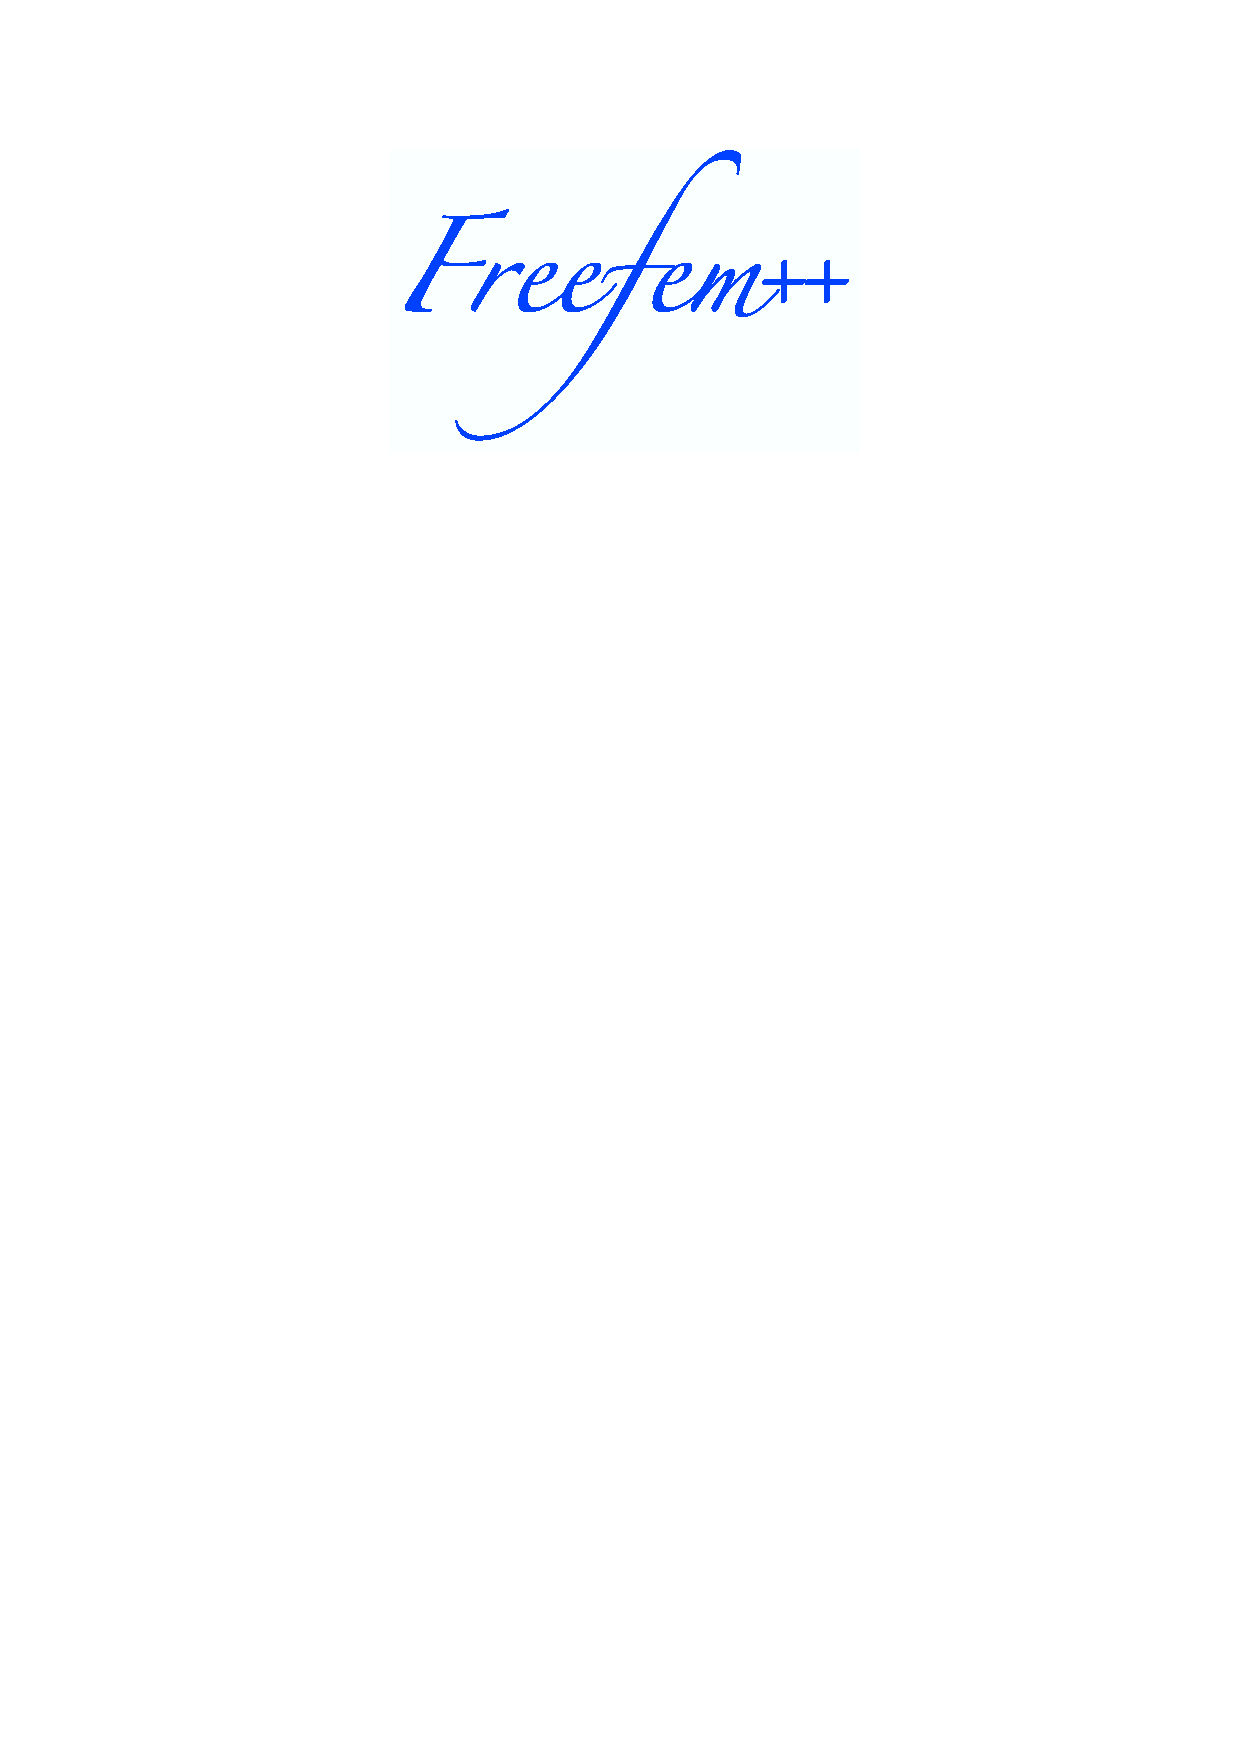
\includegraphics[width=10cm]{titre-ff}
    \\  \large  \Blue{Version 2.0-0 }
 \\ \vglue 0.7cm
  {\large \Blue{\url{http://www.freefem.org/ff++}}} \\ ~
 \\~� \\
% \Blue{{ \sc {\Huge F. Hecht,  O. Pironneau}
% \\ ~ \\
%{\Huge A. Le Hyaric, K. Ohtsuka } }}
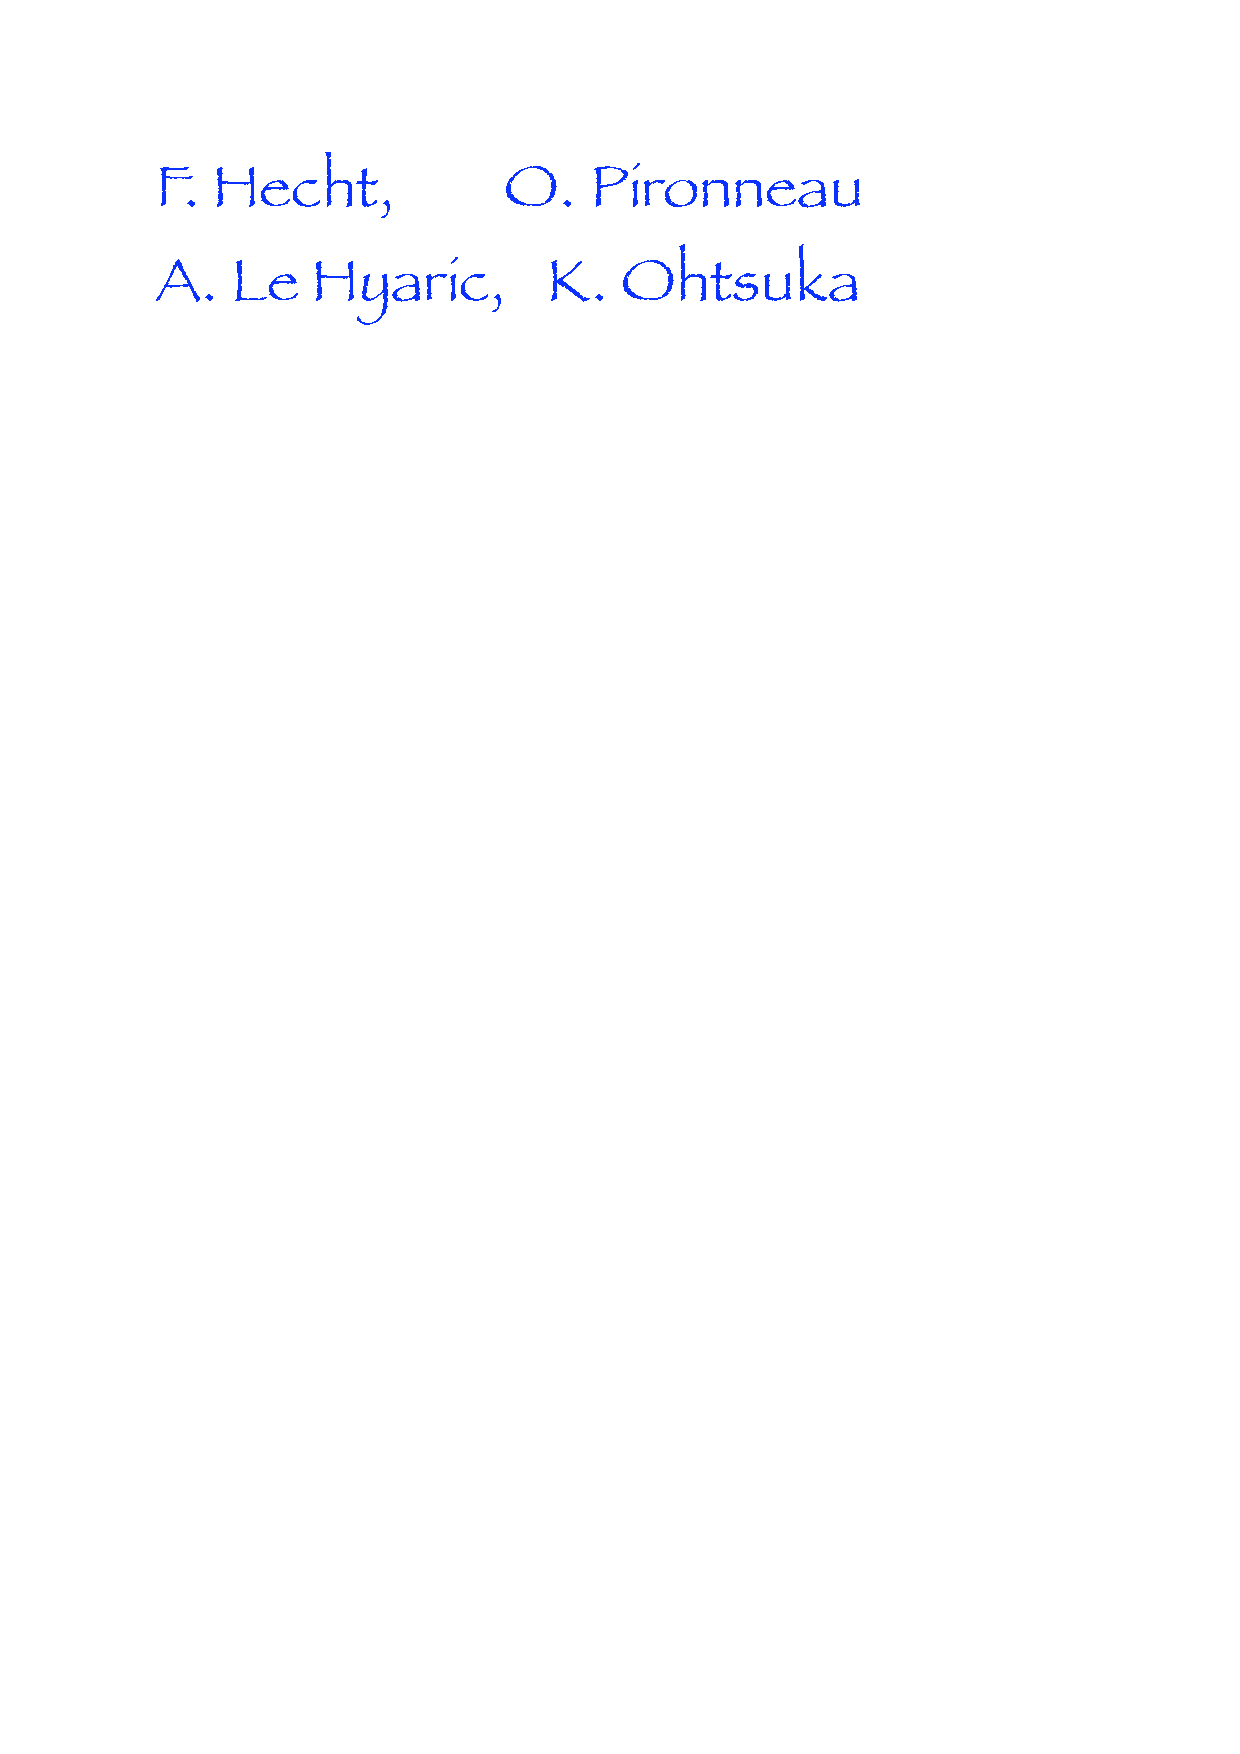
\includegraphics[width=10cm]{ffauteurs4}
\vglue 1cm
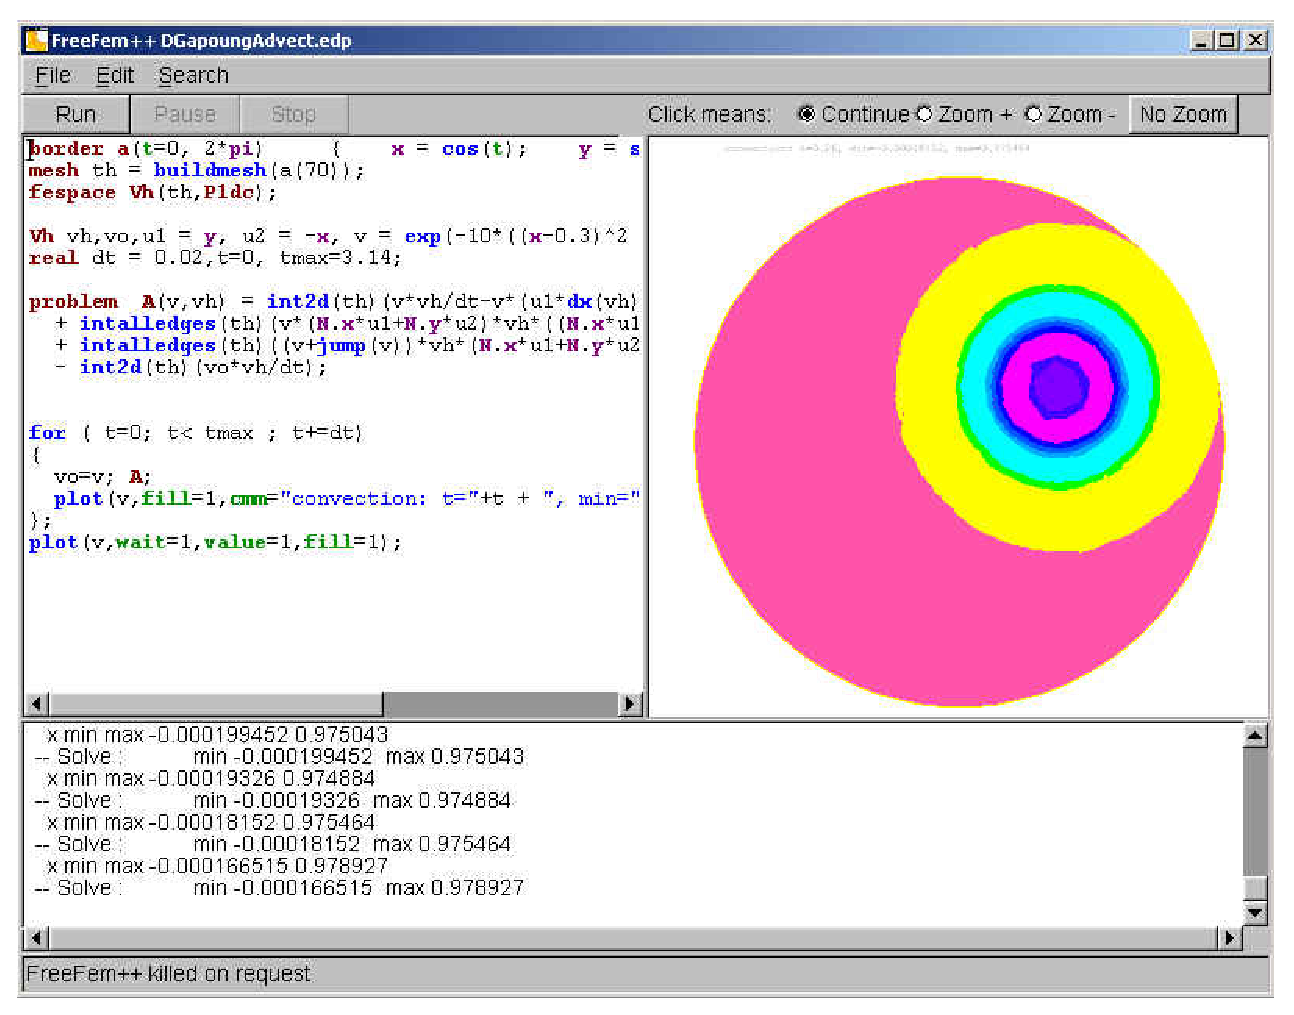
\includegraphics[width=15cm]{csSnap}
\\ \vglue0.5cm
Laboratoire Jacques-Louis Lions, Universit\'{e} Pierre et Marie Curie, Paris
\vglue-2cm
\end{center}}
\clearpage\thispagestyle{empty}\cleardoublepage
\thispagestyle{empty}
\begin{center}
 {\Blue{ \TitreFont freefem++}} \\ \vglue 1cm  ~ \\
   Version 2.0-0
 \\ \vglue 0.7cm
 {\Large \url{http://www.freefem.org/ff++}} \\
\vglue 1cm

 \
{\Large Fr\'{e}d\'{e}ric Hecht${}^{1,4}$ }

\url{mailto:frederic.hecht@upmc.fr}

\url{http://www.ann.jussieu.fr/~hecht}

\medskip

{\Large Olivier Pironneau${}^{1,3}$}

  \url{mailto:olivier.pironneau@upmc.fr}

\url{http://www.ann.jussieu.fr/pironneau}


\bigskip



{\Large Antoine Le Hyaric${}^{1,2}$ }

 \url{mailto:lehyaric@ann.jussieu.fr}

\url{http://www.ann.jussieu.fr/~lehyaric/}


\bigskip


{\Large Kohji Ohtsuka${}^{5}$ }

  \url{mailto:ohtsuka@barnard.cs.hkg.ac.jp}

\url{http://barnard.cs.hkg.ac.jp/}
\end{center}

%\bigskip


\begin{enumerate}
\item  Laboratoire Jacques-Louis Lions,
175 rue du Chevaleret , 75013 Paris, France

 Universit\'{e} Pierre et Marie Curie,
4 Place  Jussieu,  75252  PARIS cedex 05, France.


\item CNRS, UMR 7598,  Laboratoire Jacques-Louis Lions,
175 rue du Chevaleret , 75013 Paris, France.
\item Institut de France, Acad\'{e}mie des sciences, 23, quai de Conti,  75006 Paris,  France.
\item INRIA, Projet Gamma, Domaine de Voluceau, Rocquencourt, B.P. 105, 78153 Le Chesnay Cedex, France.

\item Hiroshima Kokusai Gakuin University, Hiroshima, Japan.

\end{enumerate}
\hbox to \hsize
{\hss

\includegraphics[height=2cm]{LogoLJLL} \hss

\includegraphics[height=2cm]{LogoUPMC} \hss

\includegraphics[height=2cm]{LogoCNRS} \hss
}




\cleardoublepage
%%%%%%%%%%
 \setcounter{page}{1}
\tableofcontents
\let\subsubsection\subsection
\let\subsection\section
\let\section\chapter
\section*{Preface}
\hfill{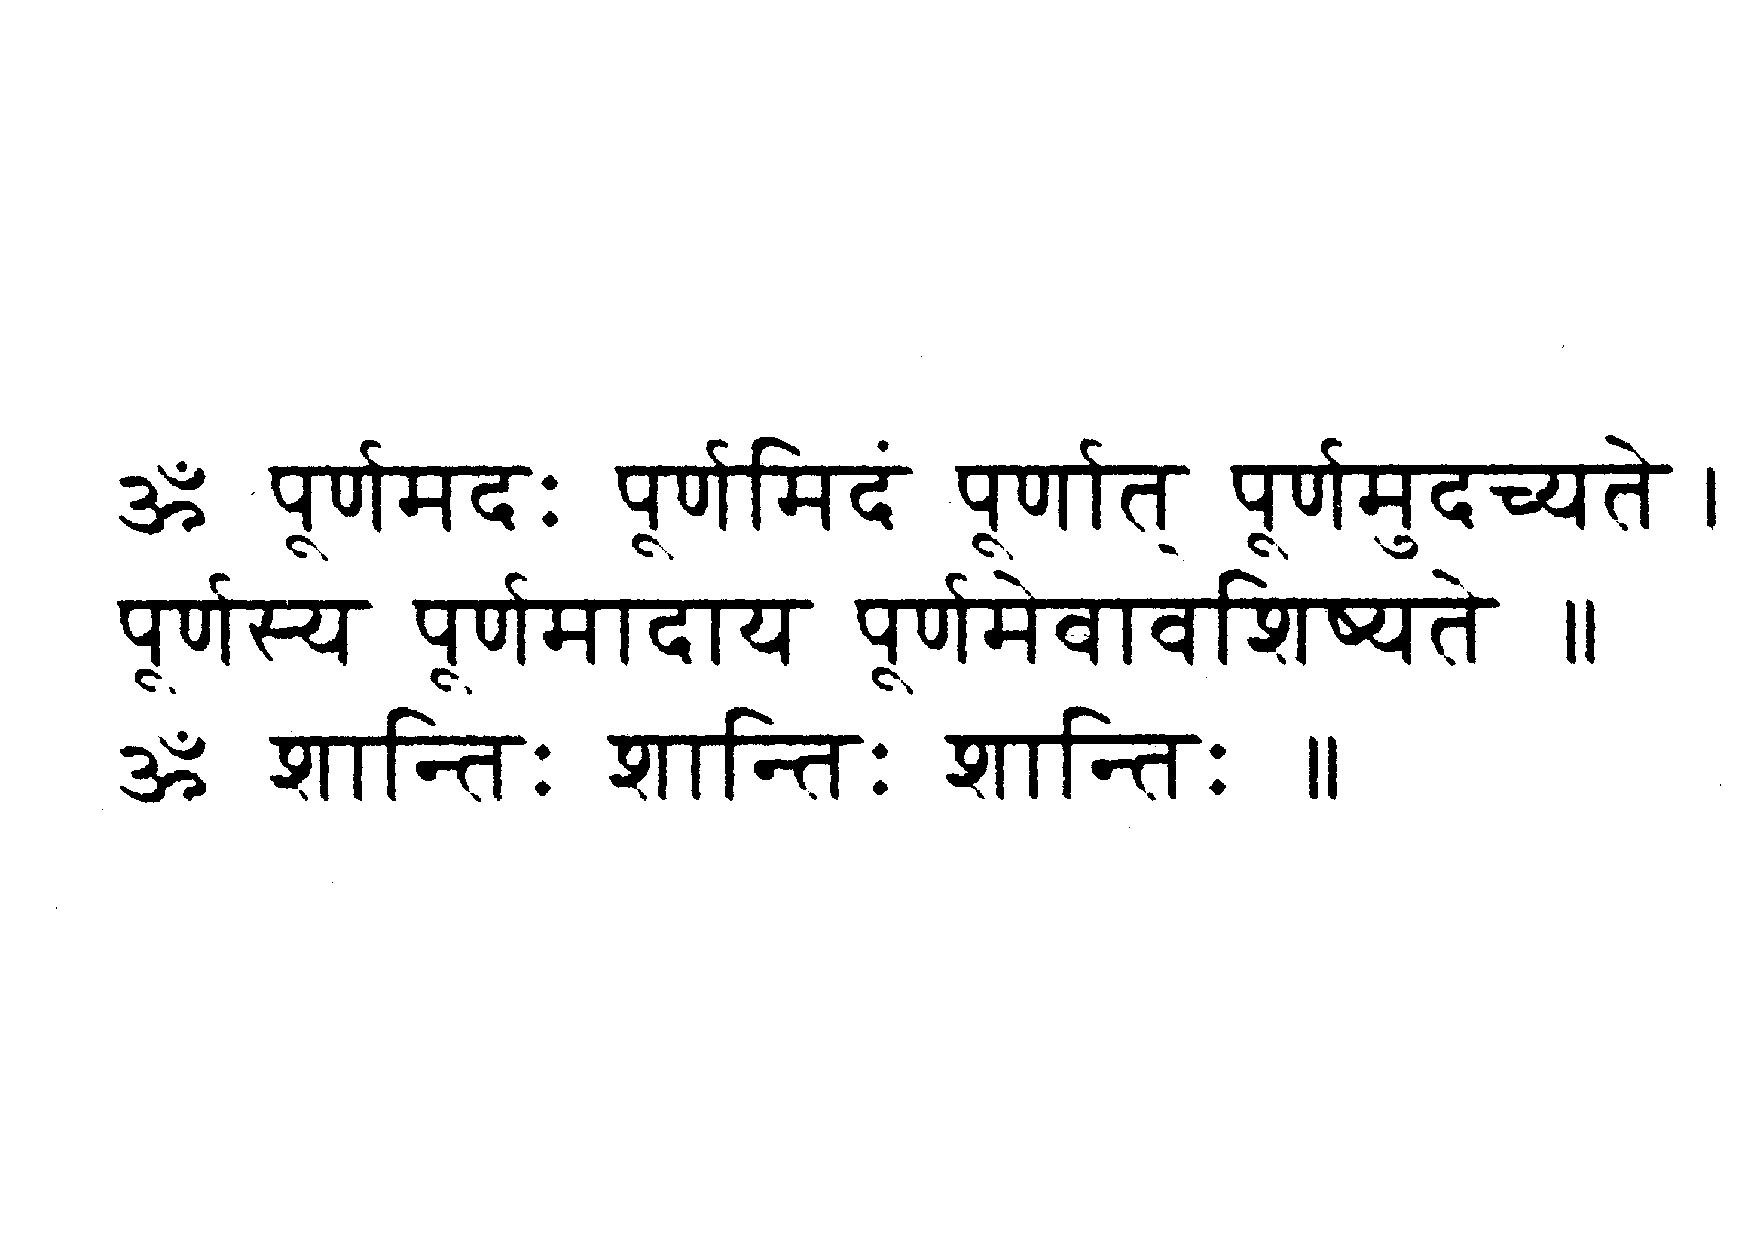
\includegraphics[height=7cm,angle=90]{sanskrit}}
\vskip 1cm

Fruit of a long maturing process freefem, in its last avatar, freefem++, is a high level integrated development environment (IDE)  for partial differential equations (PDE).  It is the ideal tool for teaching the finite element method but it is also perfect for research to quickly test new ideas or multi-physics and complex applications.
\medskip

Freefem++ has an advanced automatic mesh generator, capable of a posteriori mesh adaptation; it has a general purpose elliptic solver  interfaced with fast algorithms such as the multi-frontal method UMFPACK. Hyperbolic and parabolic problems are solved by iterative algorithms prescribed by the user with the high level language of freefem++. It has several triangular  finite elements, including discontinuous elements.  Finally everything is there in freefem++ to prepare research quality reports: color display online with zooming and other features and postscript printouts.
\medskip

This book is ideal for students at Master level, for  researchers at any level and for engineers also in financial mathematics.


\section{Introduction}\pagenumbering{arabic} \setcounter{page}{1}
A partial differential equation is a relation between a function
of several variables and its (partial) derivatives.
 Many problems in physics, engineering, mathematics and even banking
are modeled by one or several partial differential equations.
\\\\
\freefempp is a software to solve these equations numerically. As
its name says, it is a free software (see copyright for full detail)
based  on the Finite Element Method; it is not a package, it an integrated product with its own
high level programming language. This software runs on all unix
OS (with g++ 2.95.2 or better and X11R6) , on Window95, 98, 2000,
NT, XP,  on MacOS 9 and
X.  \\\\
Moreover \freefempp is highly adaptive.  Many phenomena involve
several  coupled systems: fluid-structure interactions,
Lorenz forces for aluminium casting and ocean-atmosphere problems are
three such systems. These require different finite element approximations
degrees, possibly on different meshes. Some algorithms like
Schwarz' domain decomposition method also require data interpolation
on multiple meshes within one program. \freefempp can handle these
difficulties, i.e. {\it arbitrary finite element spaces on arbitrary
unstructured and adapted bidimensional meshes}.  \\\\

The characteristics of \freefempp are:
\begin{itemize}
\item Problem description (real or complex) by their variational formulations,
with access to the internal vectors and matrices if needed.
%
\item Multi-variables, multi-equations, bi-dimensional (or 3D
axisymmetric) , static or time dependent, linear or nonlinear
coupled systems; however the user is required to describe the
iterative procedures which reduce the problem to a set of linear
problems.
%
\item Easy geometric input by analytic description of boundaries by pieces;
however this module is not a CAD system; for instance when two
boundaries intersect, the user must specify the intersection points.
%
\item Automatic mesh generator, based on the Delaunay-Voronoi
algorithm. Inner points density is proportional to the density of
points on the boundary \cite{George}.
%
\item Metric-based anisotropic mesh adaptation. The metric can be
computed automatically from the Hessian of any \freefempp function
\cite{bamg}.
%
\item High level user friendly typed input language with an algebra
of analytic and finite element functions.
%
\item  Multiple finite element meshes within one application with
automatic interpolation of data on different meshes and possible
storage of the interpolation matrices.
%
\item A large variety of triangular finite elements : linear and quadratic
 Lagrangian elements, discontinuous P1 and Raviart-Thomas elements,
 elements of a non-scalar type, mini-element, ...(no quadrangles).
%
\item Tools to define discontinuous Galerkin formulations
via the keywords: ``jump'', ``mean'', ``intalledges'').
%
\item A large variety of linear direct and iterative solvers
(LU, Cholesky, Crout, CG, GMRES, UMFPACK) and eigenvalue and
eigenvector solvers.
%
\item Near optimal execution speed (compared with compiled C++
implementations programmed directly).

\item Online graphics, generation of \texttt{,.txt,.eps,.gnu, mesh} files
  for further manipulations of input and output data.
%
\item Many examples and tutorials: elliptic, parabolic and hyperbolic problems,
 Navier-Stokes flows, elasticity, Fluid structure interactions,
Schwarz's domain decomposition method, eigenvalue problem, residual
error indicator, ...
%
\item An experimental parallel version using \texttt{mpi}
\end{itemize}

\subsection{Installation on Windows and Mac OS}

Binaries are available for Microsoft Windows and Apple
Mac OS X in the section
"\texttt{freefem++}" at \url{http://www.freefem.org}.
\\
 Unix users should download the source code and
compile it via an install/make command (see below).

\subsection{How to use \freefempp}
The executable \texttt{freefem++.exe} opens a dialog box for
choosing the input file; then it executes its content and produces
graphics and output files.
\\\\
To write or modify the input file a text editor can be used.
\\\\
An integrated environment, written by A. Le Hyaric, is also included
with the distribution (\freefempp GUI) \texttt{FreeFem++-cs.exe}; note however that
the graphics display much slower in this mode.
There are other ways to have an integrated environment. TeX users have
usually an editor installed; if it is winedt or TeXnicCenter then these can
be programmed to handle the edit-run-correct cycle of \freefempp with
color syntax and automatic launch of freefem.  If you don't have one of these
installed the easiest is to download the freeware \texttt{Crimpson Editor}.
\begin{figure}[htbp]
\begin{center}
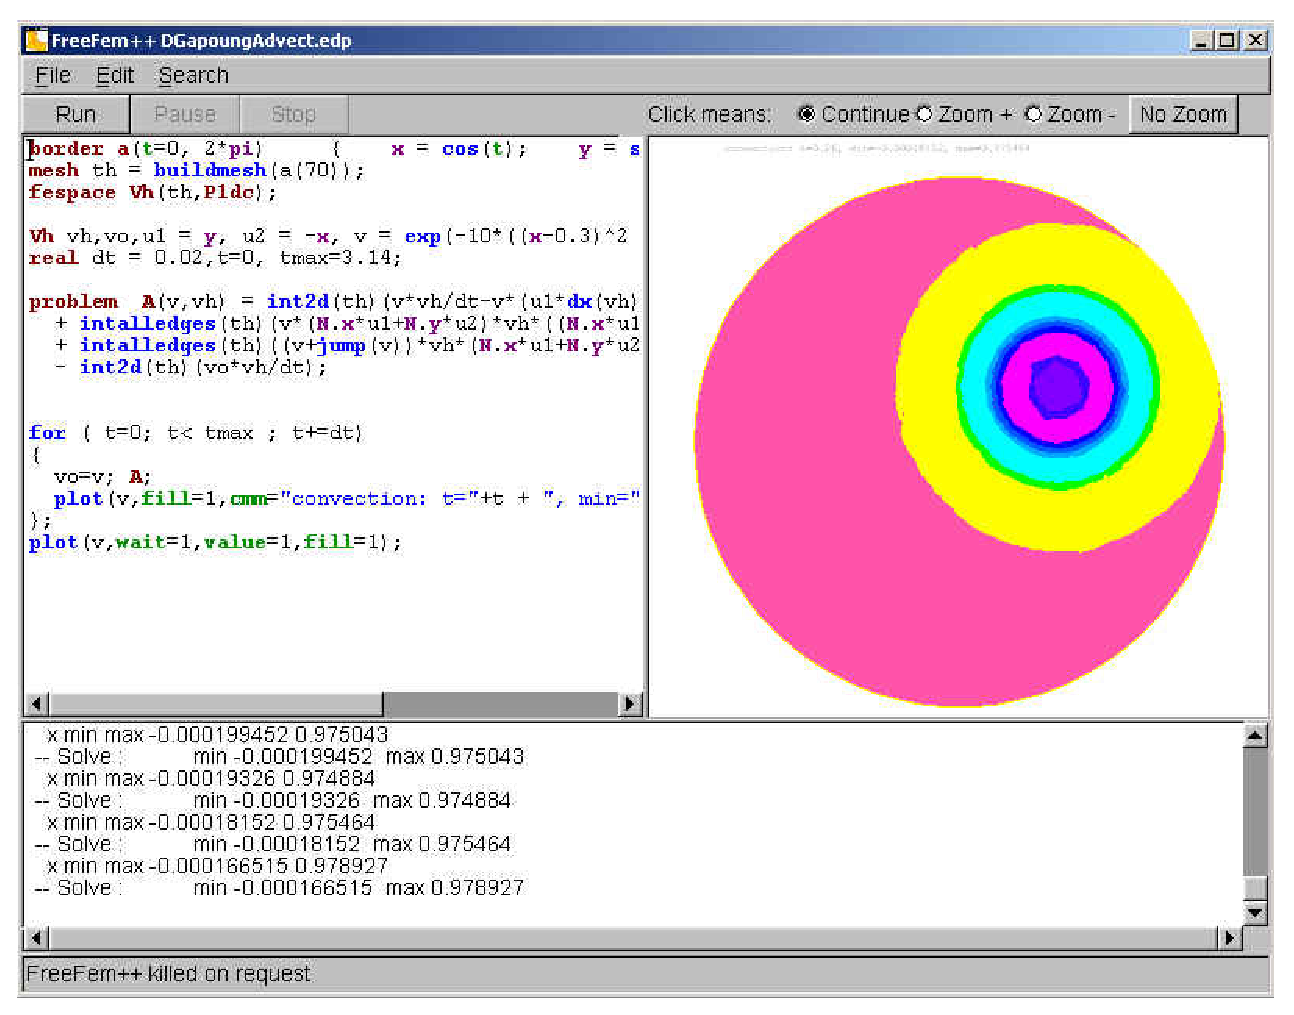
\includegraphics[width=15cm]{csSnapOld}
\caption{ The 3 panels of the integrated environment \texttt{freefem++-cs}:
to left the program, top right the graphic window, bottom the text messages.}
\end{center}
\end{figure}

\begin{description}
\item[\texttt{Crimson Editor}]
at \url{http://www.crimsoneditor.com/} and adapt it as follows:

\begin{itemize}
\item Go to the Tools/Preferences/File association menu and add the .edp extension set

\item In the same panel go to Filters and add  freefem++(*.edp) item

\item In the same panel again but under "Syntax Files"
   add two files FREEFEM.SPC and FREEFEM.KEY to define the color syntax.  To build
   the first one simply copy paste the content of JAVA.SPC as for the second
   copy paste the list of keywords in section \ref{keywrds}.

\item In the same panel in Tools/User Tools, add a freefem++ item (1st line) with the path
to freefem++.exe on the second line and \$(FilePath) and \$(FileDir on third and fourth lines.
Tick the 8.3 box.
\end{itemize}

\item[winedt] for Windows : this is the best but it could be tricky to set up.  Download it from \url{http://www.winedt.com} : this is a multipurpose text editor  with advance features
such as syntax coloring; a macro is available on ww.freefem.org to localize winedt to \freefempp
without disturbing the winedt functional mode for LateX, TeX, C, etc.  However winedt is not free
after the trial period.

\item[TeXnicCenter] for Windows: this is the easiest and will be the best once we find a volonteer
to program the color syntax.  Download it from \url{http://www.texniccenter.org/}
It is also an editor for TeX/LaTeX but it has a "`tool"' menu which can be configure to launch
\freefempp programs:  do the following:
\begin{itemize}
\item Select the Tools/Customize menu will bring a dialog box.
\item Select the "`Tools"' tab and  create a new item: call it freefem.

\item in the 3 lines below, 1/ search for FreeFem++.exe 2/ select Main file with further option  then Full path and click also on the 8.3 box 3/ select main file full directory path with 8.3
\end{itemize}
\item[nedit] on the Mac OS, Cygwin/Xfree and linux.
\end{description}
%
\begin{figure}[htbp]
\begin{center}
\includegraphics[width=15cm]{crimpson}
\caption{ The 3 panels of the integrated environment built with the
\texttt{Crimson Editor} with \freefempp in action. The Tools menu
has an item to launch \freefempp by a Ctrl+1 command.}
\end{center}
\end{figure}

\subsection{Installation on Linux/Unix machines}

For these platforms (including \texttt{cygwin}), \freefempp must be compiled and
installed from the source archive. This archive is available from:

\url{http://www.ann.jussieu.fr/~hecht/ftp/freefem/freefem++.tgz}.

 To
extract files from the compressed archive \texttt{freefem++.tgz} into
a directory called
\begin{center}
\texttt{freefem++-X.XX} (where X.XX is the version number)
\end{center}
enter the following commands in a shell window~:

\bFF
tar zxvf freefem++.tgz
cd freefem++-X.XX
\eFF

To compile and install \freefempp, just follow the \texttt{INSTALL}
and \texttt{README} files. The following programs are produced,
depending on the system you are running (Linux, Windows, MacOS)~:

\begin{enumerate}
\item \texttt{FreeFem++}, standard version, with a graphical interface
based on X11, Win32 or MacOS
\item \texttt{FreeFem++-nw}, postscript plot output only (batch version, no windows)
\item \texttt{FreeFem++-mpi}, parallel version, postscript output only
\item \texttt{FreeFem++-glx}, graphics using OpenGL and X11
\item \texttt{FreeFem++-cs}, integrated development environment
(please see chapter ``Graphical User Interface'' for more details).
\item \texttt{/Applications/FreeFem++.app}, Drag and Drop CoCoa MacOs
Application
\item \texttt{FreeFem++-CoCoa}, MacOS Shell script for MacOS OpenGL
version (MacOS 10.2 or better) (note: it uses
/Applications/FreeFem++.app)
\end{enumerate}

As an installation test, go into the directory
\texttt{examples++-tutorial} and run \freefempp on the example script
\texttt{LaplaceP1.edp} with the command~:

\bFF
FreeFem++ LaplaceP1.edp
\eFF

\subsection{History}

The project has evolved from \texttt{MacFem, PCfem}, written in
Pascal. The first C version lead to \texttt{freefem 3.4}; it offered
mesh adaptativity on a single mesh only.
\\\\
A thorough rewriting in C++ led to \texttt{freefem+}
(\texttt{freefem+ 1.2.10} was its last release), which included
interpolation over multiple meshes (functions defined on one mesh
can be used on any other mesh); this software is no longer
maintained but still in use because it handles a problem description
using the strong forms of the PDEs. Implementing the interpolation
from one unstructured mesh to another was not easy because it had to
be fast and non-diffusive; for each point, one had to find the
containing triangle. This is one of the basic problems of
computational geometry (see Preparata \& Shamos\cite{Preparata} for
example). Doing it in a minimum number of operations was the
challenge. Our implementation is $O(n\log n)$ and based on a
quadtree.  This version also grew out of hand because of the
evolution of the template syntax in C++.
 \\\\
We have been working for a few years now on \freefempp, entirely
re-written again in C++ with a thorough usage of {\tt template} and
generic programming
for coupled systems of unknown size at compile time. Like all
versions of \texttt{freefem} it has a high level user friendly input
language which is not too far from the mathematical writing of the
problems.
\\\\

The freefem language allows for a quick specification of any partial
differential system of equations.  The language syntax of \freefempp
is the result of a new design which makes use of the STL \cite{cpp},
templates and \texttt{bison} for its implementation; more detail can
be found in \cite{FHcpp}.
  The outcome is a
versatile software in which any new finite element can be included
in a few hours; but a recompilation is then necessary.  Therefore
the library of finite elements available in \freefempp will grow
with the version number and with the number of users who program
more new elements. So far we have discontinuous P$^0$
elements,linear P$^1$ and quadratic P$^2$ Lagrangian elements,
discontinuous P$^1$ and Raviart-Thomas elements and a few others like bubble elements.


\section{Getting Started}
\label{sec:example}

Let us explain how \freefempp solves the problem of
\textbf{Poisson}: \emph{For a given function $f(x,y)$, find a
function $u(x,y)$ satisfying}
\begin{eqnarray}
\label{eqn:Poisson}
-\Delta u(x,y) &=& f(x,y)\quad \mbox{ for all }(x,y)\in\Omega,\mbox{ where }
 \Delta u = \frac{\p^2 u}{\p x^2 } + \frac{\p^2 u}{\p y^2},
 \\ \label{eqn:Dirichlet}
  u(x,y) &=& 0\quad \mbox{ for all }(x,y)\mbox{ on }\p\Omega,~~\mbox{ the boundary of }\Omega.
\end{eqnarray}

The following is a \freefempp program which computes $u$ when
$f(x,y)=xy$  and $\Omega$ is the unit disk. The boundary
$C=\p\Omega$ is
$$
C=\{(x,y)|\; x=\cos(t),\, y=\sin(t),\, 0\le t\le 2\pi\}
$$
By definition the domain is on the left side of the boundary
oriented by the parameter $t$. As illustrated in Fig. \ref{firstU},
we can see the isovalue of $u$ by using \ttCC{@plot} (see line 13
below). \twoplot[height=5cm]{firstTh}{firstU}{mesh \ttCC{Th} by
\ttCC{build(C(50))}}{isovalue by \ttCC{plot(u)}}

\begin{example}\label{exm:first}~
\bFF
 1: @border C(t=0,2*@pi){@x=cos(t); @y=sin(t);}  // the triangulated domain Th
 2: @mesh Th = @buildmesh (C(50));  // is on the left side of its boundary
 3; @fespace Vh(Th,@P1); // Finite Element of degree 1 defined here for Vh
 4: Vh u,v;  // defines u and v as piecewise-P1 continuous functions
 5: @func f= x*y;  // definition of an algebraic function
 6: @real cpu=clock();
 7: @solve Poisson(u,v,@solver=LU) =  // defines the PDE
 8:    @int2d(Th)(@dx(u)*@dx(v) + @dy(u)*@dy(v))   //  bilinear part
 9:    - @int2d(Th)( f*v)          // right hand side
 10:    + @on(C,u=0)  ;  // Dirichlet boundary condition
 11: @plot(u);
 12: @cout << " CPU time = " << clock()-cpu << @endl;
\eFF
\end{example}
Note that the qualifier "solver=LU" is not required and by default a
multi-frontal LU would have been used. Note also that the lines
containing \texttt{clock} are equally not required. Finally note how
close to the mathematics \freefempp input language is. Line 6
corresponds to the mathematical variational equation
\[
    \int_{T_h}(\frac{\p u}{\p x}\frac{\p v}{\p x}
    +\frac{\p u}{\p y}\frac{\p v}{\p
    y})\d x \d y
    =
   \int_{T_h}f v\d x\d y
\]
for all $v$ which are in the finite element space $V_h$ and zero on
the boundary $C$.
\paragraph{Exercise}
Change P1 into P2 and run the program.


\subsubsection{FEM by \freefempp: how does it work?}
This first example shows how \freefempp executes  with no effort all
the usual steps required by the finite element method (FEM). Let us
go through them one by one.
\\\\
\textbf{1st line:} the boundary $\Gamma$ is described analytically
by a parametric equation for $x$ and for $y$. When
$\Gamma=\sum_{j=0}^J \Gamma_j$ then each curve $\Gamma_j$, must be
specified and crossings of $\Gamma_j$ are not allowed except at end
points .

The keyword ``label'' can be added to define a group
of boundaries for later use (boundary conditions for instance).
 Hence the circle could also have been described as two half circle with
 the same label:
 \bFF
@border Gamma1(t=0,@pi)   {@x=cos(t); @y=sin(t); @label=C}
@border Gamma2(t=@pi,2@pi){@x=cos(t); @y=sin(t); @label=C}
 \eFF
Boundaries can be referred to  either by name (Gamma1 for example) or by label (C here)
or even by its internal number here 1 for the first half circle and 2 for the second
(more examples are in \refSec{Meshing Examples}).
\\\\
\textbf{2nd line:} the triangulation $\mathcal{T}_h$ of $\Omega$ is
automatically generated  by ``\ttCC{@buildmesh}(C(50))'' using 50
points on $C$ as in Fig. \ref{firstTh}.

The domain is assumed to be on the left side of the boundary which is implicitly
oriented by the parametrization. So an elliptic hole can be added by
 \bFF
 @border C(t=2*@pi,0){@x=0.1+0.3*cos(t); @y=0.5*sin(t);}
 \eFF
If by mistake one had written
 \bFF
 @border C(t=0,2*@pi){@x=0.1+0.3*cos(t); @y=0.5*sin(t);}
 \eFF
then the inside of the ellipse would be triangulated as well as the outside.

Automatic mesh generation is
based on the Delaunay-Voronoi algorithm. Refinement of the mesh are
done by increasing the number of points on $\Gamma$, for example,
\ttCC{@buildmesh}(C(100)), because inner vertices are determined
by the density of points on the boundary. Mesh adaptation can be performed also
against a given function f by calling \ttCC{@adaptmesh}(Th,f).

Now the name $\mathcal{T}_h$ (\texttt{Th} in \freefempp) refers to
the family $\{T_k\}_{k=1,\cdots,n_t}$ of triangles shown in figure \ref{firstTh}.
Traditionally  $h$ refers to the mesh size, $n_t$ to the number of
triangles in $\mathcal{T}_h$ and $n_v$ to the number of vertices, but it is seldom
that we will have to use them explicitly.
If $\Omega$ is not a polygonal domain, a ``skin'' remains between
the exact domain $\Omega$ and its approximation
$\Omega_h=\cup_{k=1}^{n_t}T_k$.
However, we notice that all corners of $\Gamma_h = \p\Omega_h$ are
on $\Gamma$.
\\\\
\textbf{3rd line:} A finite element space is, usually, a space of
polynomial functions on elements, triangles here only, with certain matching properties
at edges, vertices etc.  Here \ttCC{@fespace Vh(Th,P1)} defines $V_h$ to be the
space of continuous functions which are affine in $x,y$ on each triangle of $T_h$.  As it is a
linear vector space of finite dimension, basis can be found.
The canonical basis is made of functions, called the \index{hat function}\emph{hat functions}
$\phi_k$ which are continuous piecewise affine and are equal to 1 on one vertex and 0 on all others.
A typical hat function is shown on figure \ref{fig-hatFunction}
\footnote{
The easiest way to define $\phi_k$ is by making use of the \index{barycentric coordinates}
\emph{barycentric coordinates}
$\lambda_i(x,y),~i=1,2,3$ of a point $q=(x,y)\in T$, defined by
\[
    \sum_i\lambda_i=1,~~~\sum_i\lambda_i\vec q^i=\vec q
\]
where $q^i,~i=1,2,3$ are the 3 vertices of T.  Then it is easy to see that
the restriction of $\phi_k$ on $T$ is precisely $\lambda_k$.
}.
Then
\begin{equation}
V_h(\mathcal{T}_h,P_1)=\left\{w(x,y)\left|\;
w(x,y)=\sum_{k=1}^{M}w_k\phi_k(x,y),\, w_k\textrm{ are real numbers}\right.\right\}
\end{equation}
where $M$ is the dimension of $V_h$, i.e. the number of vertices.
The $w_k$ are called the \index{degree of freedom}\emph{degree of freedom} of $w$ and $M$ the number of
the degree of freedom.
\begin{figure}[htbp]\label{fig-hatFunction}
\begin{minipage}{\textwidth}
\begin{minipage}{0.3\textwidth}
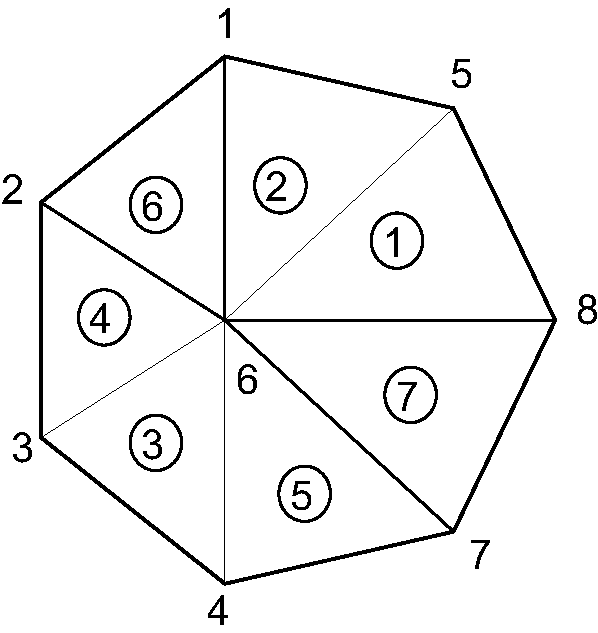
\includegraphics[width=\textwidth]{secondT}%
\caption{mesh \texttt{Th}}
\end{minipage}
\hspace{0.5mm}
\begin{minipage}{0.7\textwidth}
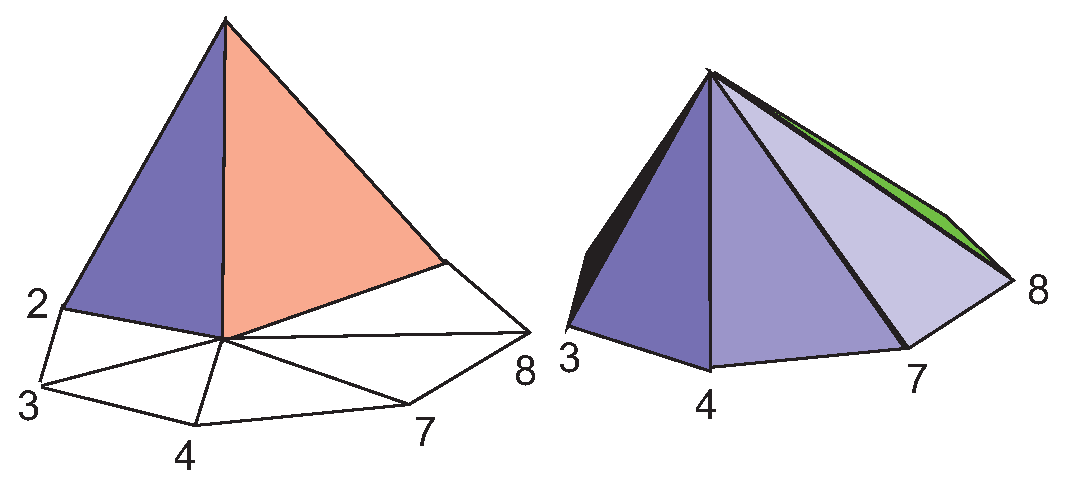
\includegraphics[width=\textwidth]{hat}%
\caption{Graph of $\phi_1$ (left hand side) and $\phi_6$}
\end{minipage}
\end{minipage}
\end{figure}
It is said also that the \index{nodes}\emph{nodes} of this finite element method
are the vertices.
\\
Currently \freefempp implements the following elements \index{elements}
\begin{description}
\item{P0} piecewise constant,
\item{P1} continuous piecewise linear,
\item{P2} continuous piecewise quadratic,
\item{RT0} Raviart-Thomas piecewise constant,
\item{P1nc} piecewise linear non-conforming,
\item{P1dc} piecewise linear discontinuous,
\item{P2dc} piecewise quadratic discontinuous,
\item{P1b} piecewise linear continuous plus bubble,
\item{P2b} piecewise quadratic continuous plus bubble.
\end{description}
The user can  add other elements fairly easily if required.
\\\\
\textbf{Step3: Setting the problem}
\\
\textbf{4th line:} ``\texttt{Vh u}'' declare that $u$ is approximated as above,
nmely
\begin{equation}\label{defu}
u(x,y)\simeq u_h(x,y)=\sum_{k=0}^{M-1} u_k\phi_k(x,y)
\end{equation}
\textbf{5th line:} the right hand side $f$ is defined analytically using the keyword
\ttCC{@func}.

\textbf{7th--9th lines:} defines the bilinear form of the (\ref{eqn:Poisson}) and
its Dirichlet boundary conditions (\ref{eqn:Dirichlet}).
\\
This \emph{variational formulation} is derived by
multiplying (\ref{eqn:Poisson}) by $v(x,y)$ and integrating
the result over $\Omega$:
$$
-\int_{\Omega}v\Delta u \,\d x\d y = \int_{\Omega} vf\, \d x\d y
$$
Then, by Green's formula, the problem  is converted into finding $u$
such that
\begin{eqnarray}
\label{eqn:weakform}
&&a(u,v) - \ell(f,v) = 0\hbox{ satisfying $v=0$ on }\p\Omega.
\qquad \textrm{for all }v\\
&&\hbox{with }a(u,v)=\int_{\Omega}\nabla u\cdot \nabla v \,\d x\d y
\quad \ell(f,v)=\int_{\Omega}fv\, \d x\d y
\label{eqn:bilinear}
\end{eqnarray}
 In \freefempp
the problem \textbf{Poisson} can be  declared only (see below) or
declared and solved in which case
\begin{center}
\ttCC{Vh u,v; @solve Poisson(u,v) =}
\end{center}
and (\ref{eqn:weakform}) is written with \ttCC{@dx}(u) $=\p
u/\p x$, \ttCC{@dy}(u) $=\p u/\p y$ and
\begin{eqnarray*}
&&\int_{\Omega}\nabla u\cdot \nabla v\, \d x\d y \longrightarrow
\ttCC{@int@2d(Th)( @dx(u)*@dx(v) + @dy(u)*@dy(v) )}\\
&&\int_{\Omega}fv\, \d x\d y \longrightarrow
\ttCC{@int@2d(Th)( f*v )}\qquad
\textrm{(notice here, $u$ is unused)}\\
\end{eqnarray*}
In \freefempp there is no need to differentiate between $a$ and
$\ell$, as lomng as the terms are inside different integrals, it
finds which is which by checking where $u$ is present or
not.
\\\\
\textbf{Step4: Solution and visualization}\\

\textbf{6th line:} The current time is stored into the real-valued variable \ttCC{cpu}.

\textbf{7th line} The problem is solved

\textbf{11th line:} The visualization is done as illustrated in Fig. \ref{firstU}
(see \refSec{Plot} for zoom, postscript and other commands).

\textbf{12th line:} The computing time (not counting graphics) is written on the console
Notice the C++-like syntax; the user needs not study C++ for using \freefempp,
but it helps to guess what is allowed in the language.
\\\\
\textbf{Access to matrices and vectors}
\\
Internally \freefempp will solve a linear system of the type
\begin{eqnarray}
\label{eqn:Equation}
A_{ij}u_j - F_i=0\quad i,j=0,\cdots,M-1;\qquad
F_i=\int_{\Omega}f\phi_i\, \d x\d y
\end{eqnarray}
which is found by using (\ref{defu}) and replacing $v$ by $\phi_i$
in (\ref{eqn:weakform}).  The Dirichlet conditions are implemented by penalty
namely by setting $A_{ii}=tgv$ (very large value) and replacing $F_i$
by $F_i tgv$ if $q^i$ is a Dirichlet node.
\\
The matrix $A=(A_{ij})$ is called
\emph{stiffness matrix} \index{matrix!stiffness matrix} and is
modified from
\\\\
If the user wants to access $A$ directly he can do so
by using
\bFF
@varf a(u,v) = @int2d(Th)( @dx(u)*@dx(v) + @dy(u)*@dy(v))
               + @on(C,u=0) ;
@matrix A=a(Vh,Vh);  // stiffness matrix,
\eFF

The vector $F$
in (\ref{eqn:Equation}) can also be constructed manually
\bFF
@varf b(u,v) = @int2d(Th)(u*v);
@matrix B=b(Vh,Vh);
Vh v=f; F[] = B*v[];
\eFF
The problem can then be solved at the level of algebra by
\bFF
 u[]=A^-1*F[];
\eFF
The linear system (\ref{eqn:Equation}) is solved by \texttt{UFMPACK}
unless mentioned specifically like in
\begin{center}
\ttCC{Vh u,v; @problem Poisson(u,v,@solver=CG) = @int2d(...}
\end{center}
meaning that Poisson is declared only here and when it is called (by simply writing \texttt{Poisson}) then
 (\ref{eqn:Equation}) will be solved by the Conjugate Gradient method.

\subsubsection{Some Features of \freefempp}

The language of \freefempp is typed, polymorphic and reentrant with macro generation (see
\ref{macro}).  Every variable must be typed and declared in a
statement; each statement separated from the next by a semicolon;
The syntax is that of C++ by default augmented with something that is more akin
to \TeX.  For the specialist, one key guideline is that \freefempp hardly generates an internal
finite element function or array; this was adopted for speed and
consequently \freefempp could be hard to beat in terms of execution speed, except
for the time lost in the interpretation of the language (which can be reduced by a systematic usage
of \texttt{varf} and matrices instead of \texttt{problem}.


\subsubsection{\setS{Matrix Operations}}

The multiplicative operators *, /, and \% group left to right.

\begin{itemize}
\item  \verb@'@  is unary right transposition of array, matrix \index{transpose}
 \item \verb@.*@ is the term to term multiply operator. \index{.*} \index{\string'} \index{divide!term to term}
 \item \verb@./@ is the term to term divide operator. \index{./} \index{\string'} \index{product!term to term}
\end{itemize}
there are some compound operator:
\begin{itemize}
 \item \verb@^-1@ is for  solving the linear system (example: \verb$ b = A^-1 x$) \index{solve!linear system}
 \item \verb@' *@ is the compound  of transposition and matrix product, so it is the dot product
(example \verb$real DotProduct=a'*b$) \index{dot product}\index{product!dot}
\end{itemize}
\begin{example}~
\bFF
@mesh Th = @square(2,1);
@fespace Vh(Th,P1);
Vh f,g;
f = x*y;
g = sin(pi*x);
Vh<complex> ff,gg; // a complex valued finite element function \index{FE function!complex}\index{complex}
ff= x*(y+1i);
gg = exp(pi*x*i);
@varf mat(u,v) =
  int2d(Th)(1*dx(u)*dx(v)+2*dx(u)*dy(v)+3*dy(u)*dx(v)+4*dy(u)*dy(v))
  + on(1,2,3,4,u=1);
@varf mati(u,v) =
  int2d(Th)(1*dx(u)*dx(v)+2i*dx(u)*dy(v)+3*dy(u)*dx(v)+4*dy(u)*dy(v))
  + on(1,2,3,4,u=1);
@matrix A = mat(Vh,Vh); @matrix<complex> AA = mati(Vh,Vh); // a complex sparse matrix \index{matrix!complex}

Vh m0; m0[] = A*f[];
Vh m01; m01[] = A'*f[];
Vh m1; m1[] = f[].*g[];
Vh m2; m2[] = f[]./g[];
@cout << "f = " << f[] << @endl;
@cout << "g = " << g[] << @endl;
@cout << "A = " << A << @endl;
@cout << "m0 = " << m0[] << @endl;
@cout << "m01 = " << m01[] << @endl;
@cout << "m1 = "<< m1[] << @endl;
@cout << "m2 = "<< m2[] << @endl;
@cout << "dot Product = "<< f[]'*g[] << @endl;
@cout << "hermitien Product = "<< ff[]'*gg[] << @endl;
\eFF

On the triangulation of Figure \ref{fig-hatFunction} this produce the following:
\begin{eqnarray*}
A&=&\borderarray{[}{]}{1em}{1.2ex}{rrrrrrrr}{
&1&2&3&4&5&6\\
1&10^{30}& 1 0.5& 0&3 0.& 4 -2.5& 0\\
2&0.&10^{30}&0.5& 0&0.5&-2.5\\
3&0&0.&10^{30}& 0& 0&0.5\\
4&0.5& 0& 0& 10^{30}& 0.& 0\\
5&-2.5&0.5& 0&0.5&10^{30}&0.\\
6&0&-2.5&0.& 0&0.5& 10^{30}
}
\\
\{v\}=\texttt{f[]}&=&
\left(
\begin{array}{rrrrrr}
0 & 0 & 0 & 0 & 0.5 & 1
\end{array}
\right)^T\\
\{w\}=\texttt{g[]}&=&
\left(
\begin{array}{rrrrrr}
0 &1  &1.2\times 10^{-16}& 0 & 1 & 1.2\times 10^{-16}
\end{array}
\right)^T\\
\texttt{A*f[]}&=&
\left(
\begin{array}{rrrrrr}
-1.25 &  -2.25 &  0.5   & 0 & 5\times 10^{29} & 10^{30}
\end{array}
\right)^T\quad (=A\{v\})\\
\texttt{A'*f[]}&=&
\left(
\begin{array}{rrrrrr}
-1.25 &  -2.25 &  0  & 0.25 & 5\times 10^{29} & 10^{30}
\end{array}
\right)^T\quad (=A^T\{v\})\\
\texttt{f[].*g[]}&=&
\left(
\begin{array}{rrrrrr}
0 & 0 & 0 & 0 & 0.5 & 1.2\times 10^{-16}
\end{array}
\right)^T\quad =(v_1w_1\quad\cdots\quad v_Mw_M)^T\\
\texttt{f[]./g[]}&=&
\left(
\begin{array}{rrrrrr}
-nan & 0  & 0  & -nan  & 0.5 & 8.1\times 10^{15}
\end{array}
\right)^T\quad =(v_1/w_1\,\cdots\, v_M/w_M)^T\\
\texttt{f[]'*g[]}&=&0.5\quad
(=\{v\}\{w\}^T=\{v\}\cdot\{w\})
\end{eqnarray*}
\end{example}
\begin{note}
The operators \verb|^-1| cannot be used to create a matrix;
the following gives an error
\bFF
@matrix AAA = A^-1;
\eFF
\end{note}

\subsection{The Development Cycle: Edit--Run/Visualize--Revise}

An integrate environment is provided with \freefempp written by A. Le Hyaric;
Many examples and tutorials are also given along with this documentation and it is best
to study them and learn by example.
Explanations for some of these examples are given in this book in the next chapter. If you are a
beginner of FEM, you may want to read also a book on variational formulations.

The development cycle will have the following steps:
\begin{description}
\item[Modeling:] From strong forms to weak form, one must know the variational formulations
to use \freefempp; one should also have an eye on the reusability of the variational
formulation so as to keep the same internal matrices; a typical example is the
time dependent heat equation with an implicit time scheme: the internal matrix can be factorized
only once and \freefempp can be taught to do so.

\item[Programming:] Write the code in \freefempp language using a text editor such as the one
provided in the integrated environment.

\item[Run:] Run the code (e.g. written in file mycode.edp).
If not from the integrated environment it can be done at the console level by

\texttt{\% freefem++ mycode.edp}

\item[Visualization:] Use the keyword \texttt{plot} to display functions while \freefempp is running.
Use the plot-parameter \texttt{wait=1} to stop the program to have time to see the plot. Use the
plot-parameter \texttt{ps="toto.eps"} to generate a postscript file to archive the results.

\item[Debugging:] A global variable "debug" (for example) can help as in
 \ttCC{@wait=@true} to \ttCC{@wait=@false}.
\bFF
@bool debug = true;
mesh Th = @square(10,10,[-1+2*x,-1+2*y]); // $]-1,1[^2$ with 10x10 mesh
@plot(Th,wait=debug);  // plot Th then needs a mouse click
@fespace Vh(Th,P2);
Vh f = @sin(pi*x)*@cos(pi*y);
plot(f,wait=debug);  // plot the function f
Vh g = @sin(@pi*x + @cos(@pi*y));
@plot(g,wait=debug);  // plot the function g
\eFF
Changing debug to false will make the plots flow continuously; drinking coffee and watching the flow of graph
on the screen can then become a pleasant experience.

Error messages are displayed in the console window. They are not always very explicit because of the
template structure of the C++ code, sorry!  Nevertheless they are displayed at the right place.
For example, if you forget parenthesis as in
\bFF
@bool debug = true;
@mesh Th = @square(10,10;
@plot(Th);
\eFF
then you will get the following message from \texttt{freefem++},
\bFF
mesh Th = square(10,10;
 Error line number 1, in file mycode.edp, before  token ;
parse error
Compile error : parse error
        line number :1, ;
 at exec line  1
error Compile error : parse error
        line number :1, ;
\eFF
If you use the same symbol twice as in
\bFF
@real aaa =1;
@real aaa;
\eFF
then you will get the message
\bFF
real aaa =1;
    1 : real aaa; The identifier aaa exist
\eFF
Notice that the line number start from 0.
If you find that the program isn't doing what you want you may also use \ttCC{@cout}
to display in text format on the console window what every is needed.  The following works
\bFF
...;
@fespace Vh...; Vh u;...
cout<<u;...
@matrix A=a(Vh,Vh);...
cout<<A;
\eFF
Another trick is to \emph{comment in and out} by using the``\ttCC{//}'' as in C++.
For example
\bFF
@real aaa =1;
// real aaa;
\eFF
\end{description}
\textBlack

\section{Learning by Examples}
This chapter is for those, like us, who don't like manuals. A number of simple examples
cover a good deal of the capacity of \freefempp and are self-explainatory.  For the modelling part
this chapter continues at Chapter 9 where the PDes of physics and engineering (and finance) are studied
in greater depth.
\subsection{Membranes}
\paragraph{Summary} \emph{Here we shall learn how to solve a \x{Dirichlet} and/or
\x{mixed Dirichlet Neumann} problem for the \x{Laplace operator} with
application to the equilibrium of a \x{membrane} under load.  We shall
also check
the \x{accuracy} of the method and interface with other \x{graphics packages}.}\\\\

An elastic membrane $\Omega$ is glued to a planar rigid support
$\Gamma$, but a force $f(x) dx$ presses on each surface element
$\d{x}=\d{x}_1 \d{x}_2$. The vertical membrane displacement,
$\varphi(x)$, is  obtained by solving  Laplace's equation:
 $$
     -\Delta \varphi =f ~\hbox{~in~}~ \Omega.
 $$
As the membrane is glued to its planar support, one has:
$$ \varphi |_{\Gamma }=0.$$
If the support wasn't planar but at an elevation $z(x_1,x_2)$ then
the boundary condition would be of \x{non-homogeneous Dirichlet}
type.
$$ \varphi|_{\Gamma}=z.$$

If a part $\Gamma_2$ of the membrane border $\Gamma$ is not glued to
the support but left hanging then due to rigidity the angle with the
nornal vector is zero; thus the boundary conditions are
$$
    \varphi|_{\Gamma_1}=z,~~~~\frac{\p\varphi}{\p n}|_{\Gamma_2}=0
$$
where $\Gamma_1=\Gamma-\Gamma_2$; recall that $\p\varphi\p
n=\n\varphi\cdot n$. Let us recall also that the Laplace operator
$\Delta$ is defined by:
 $$
    \Delta \varphi = {\p ^{2}\varphi \over \p x^{2}_{1} }
    + {\p ^{2}\varphi \over \p x_{2}^{2} }.
 $$
With such "mixed boundary conditions" the problem has a unique
solution (see (1987), Dautray-Lions (1988), Strang (1986) and
Raviart-Thomas (1983)); the easiest proof is to notice that
$\varphi$ is the state of least energy, i.e. minimizes
 $$
    \min_{\varphi-z\in V} E=\int_\Omega(\frac12|\n\varphi|^2-f\varphi)
 $$
where  $V$ is the subspace of the Sobolev space $H^1(\Omega)$ of
functions which have zero trace on $\Gamma_1$. Recall that
($x\in\R^d,~d=2$ here)
$$
    H^1(\Omega)=\{u\in L^2(\Omega)~:~\n u\in L^(\Omega)^d\}
$$
Calculus of variation shows that the minimum must satisfy, what is known as the \x{weak form}
of the PDE or its
\x{variational formulation}  (also known here as the theorem of virtual work)
$$
    \int_\Omega(\n\varphi\cdot\n w = \int_\Omega f w\quad\forall w\in V
$$
Next an integration by part (Green's formula) will show that this is equivalent to
the PDE when second derivatives exist.

\paragraph{WARNING}
Unlike \texttt{freefem+} which had both weak and strong forms, \freefempp implements only
weak formulations.  It is not possible to go further in using this software if you don't know
the weak form (i.e. variational formulation) of your problem: either you read a book, or
ask help form a colleague or drop the matter.  Now if you want to solve a system of PDE
like $A(u,v)=0,~ B(u,v)=0$ don't close this manual, because in weak form it is
$$
    \int_\Omega(A(u,v)w_1+B(u,v)w_2)=0~~\forall w_1,w2...
$$

\paragraph{Example}

Let an ellipse have principal radius $b=2$, and unitary secondary radius
Let the surface force be $f=1$. Programming this case with
\freefempp gives:
%
\begin{example}[membrane.edp]
\bFF
// file membrane.edp
@real a=4*pi/3, b=2;
@func z=x;

@border Gamma1(t=0,a)    { x = b * cos(t); y = sin(t); }
@border Gamma2(t=a,2*pi) { x = b * cos(t); y = sin(t); }
@mesh Th=@buildmesh(Gamma1(20)+Gamma2(10));

@fespace Vh(Th,P2); // P2 conforming triangular FEM
Vh phi,w, f=1;

@solve Laplace(phi,w)=@int2d(Th)(@dx(phi)*@dx(w) + @dy(phi)*@dy(w))
                - @int2d(Th)(f*w) + @on(Gamma1,phi=z);
@plot(Th,phi,wait=true,ps="membrane.eps"); //Plot Th and v
\eFF
\end{example}
\begin{figure}[htbp]\label{figmembrane}
\begin{center}
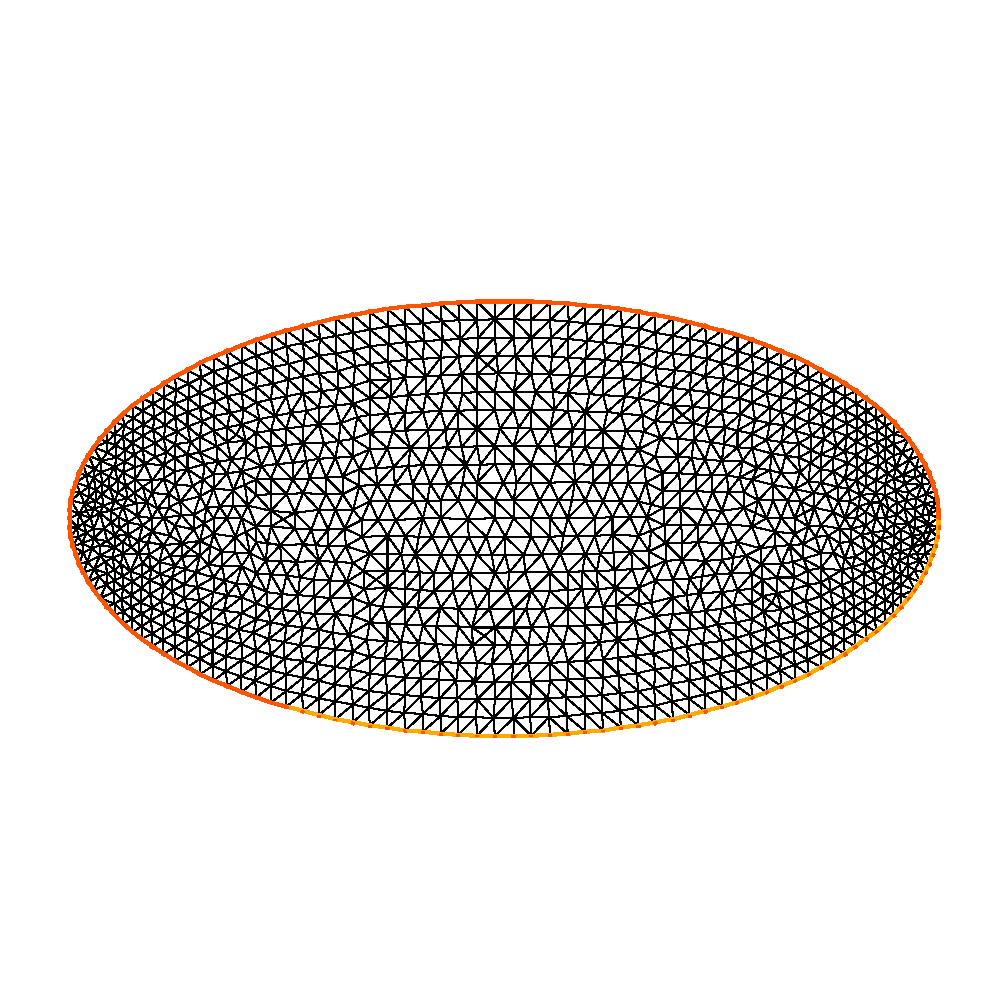
\includegraphics[width=7cm]{membraneTh}~~~
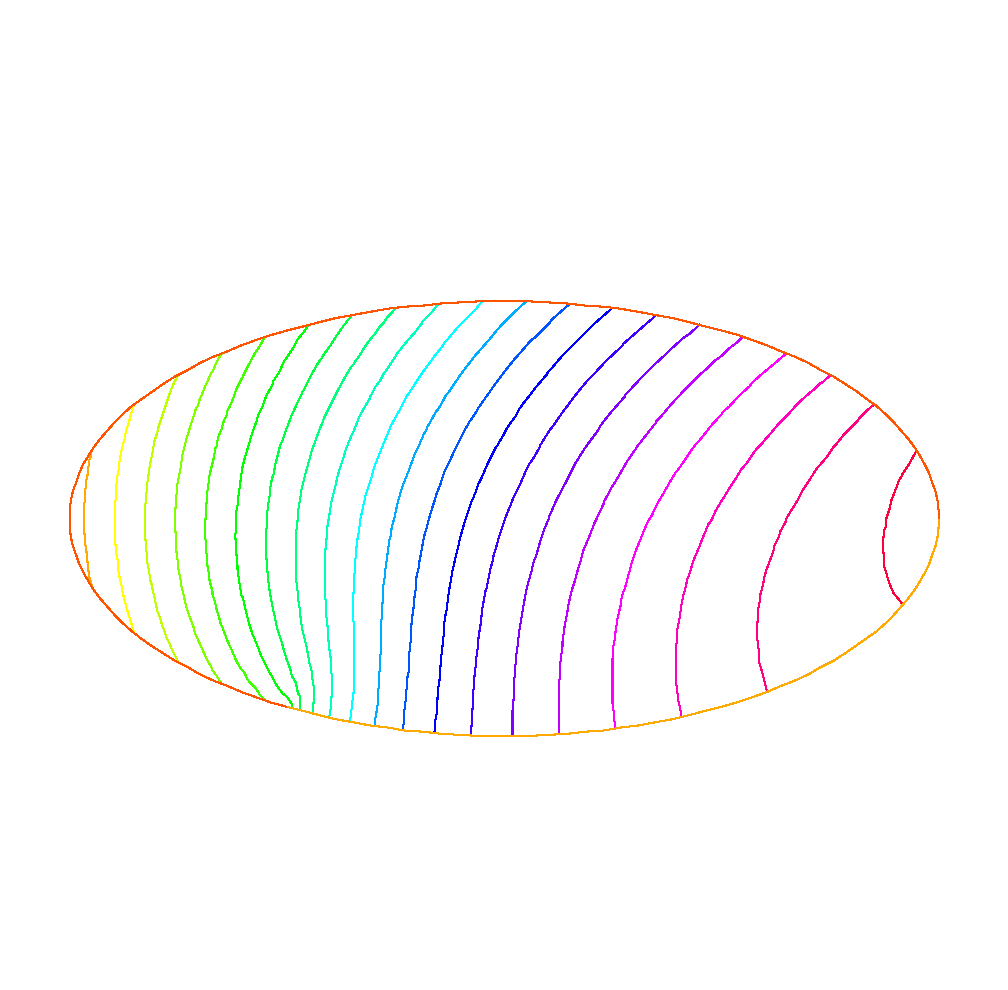
\includegraphics[width=7cm]{membrane}\\
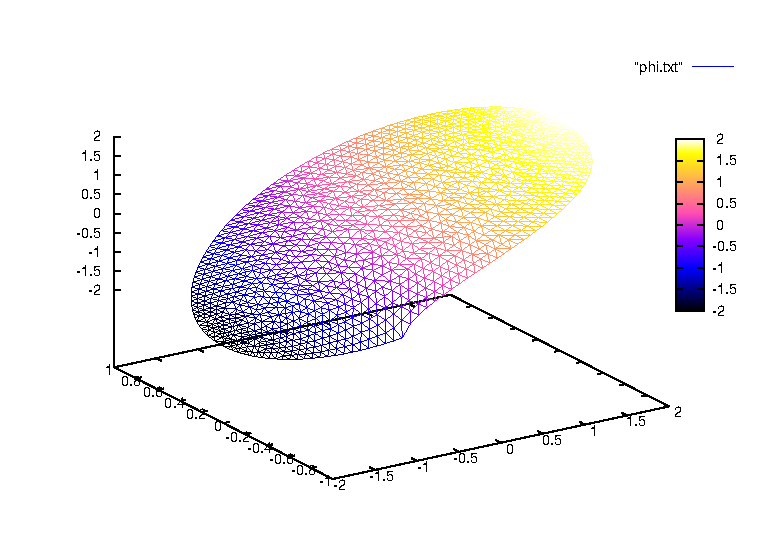
\includegraphics[width=12cm]{gnumembrane}\\
\caption{ Mesh and level lines of the membrane deformation. Below: the same in 3D
drawn by \texttt{gnuplot} from a file generated by \freefempp.}
\end{center}
\end{figure}

A triangulation is built by the keyword {\it buildmesh}. The keyword
calls a triangulation subroutine based on the Delaunay test, which
first triangulates with only the boundary points, then adds internal
points by subdividing the edges. How fine  the triangulation becomes is controlled
by the size of the closest boundary edges.
\\\\
The PDE is then discretized using the triangular second order finite
element method on the triangulation; as was briefly indicated in the previous chapter,
a linear system is derived from the discrete formulation whose size is the number of vertices
plus mid-edges in
the triangulation. The system is solved by a multi-frontal Gauss LU factorization
implemented in the package \texttt{UMFPACK}. The keyword plot will display both
$\T_h$ and $\varphi$ (remove \texttt{Th} if $\varphi$ only is desired) and the
qualifier \texttt{fill} replaces the default option (colored level lines) by a full color display.
Results are on figure \ref{figmembrane}.
\\\\
Next we would like to check the results!
\\
One simple way is to adjust the parameters so as to know the solutions.  For instance
on the unit circle (b=1), $\varphi_e=\sin(x^2+y^2-1)$ solves the problem when
\[
    z=0,~f=-4(\cos(x^2+y^2)-1)-(x^2+y^2)\sin(x^2+y^2-1)
\]
except that on $\Gamma_2$ $\p_n\varphi=2$ instead of zero.  So we will consider
a non-homogeneous Neumann condition and solve
$$
    \int_\Omega(\n\varphi\cdot\n w = \int_\Omega f w+\int_{\Gamma_2}2w\quad\forall w\in V
$$
We will do that with two triangulations, compute the $L^2$ error:
\[
\epsilon = \int_\Omega|\varphi-\varphi_e|^2
\]
and print the errors in both cases as well as the log of their ration which is by definition
the rate of convergence.
\begin{example}[membranerror.edp]\label{membran}
\bFF
// file membranerror.edp
@real a=4*pi/3, b=1;
@func f=-4*(cos(x^2+y^2-1) -(x^2+y^2)*sin(x^2+y^2-1));
@func phiexact=sin(x^2+y^2-1);
@border Gamma1(t=0,a)    { x = b * cos(t); y = sin(t); }
@border Gamma2(t=a,2*pi) { x = b * cos(t); y = sin(t); }
@mesh Th=@buildmesh(Gamma1(20)+Gamma2(10));
@fespace Vh(Th,P2);  Vh phi,w;
@solve laplace(phi,w)=@int2d(Th)(@dx(phi)*@dx(w) + @dy(phi)*@dy(w))
  - @int2d(Th)(f*w) - @int1d(Th,Gamma2)(2*w)+ @on(Gamma1,phi=0);
@plot(Th,phi,wait=true,ps="membrane.eps"); //Plot Th and v
@real L2error0 = @int2d(Th)((phi-phiexact)^2);
////////////// mesh twice finer ////////////
@int n=2;
@mesh Th1=@buildmesh(Gamma1(20*n)+Gamma2(10*n));
@fespace V1h(Th1,P2); // P2 conforming triangular FEM
V1h phi1,w1;
@solve lapl(phi1,w1)=@int2d(Th1)(@dx(phi1)*@dx(w1) + @dy(phi1)*@dy(w1))
  -@int2d(Th1)(f*w1)-@int1d(Th1,Gamma2)(2*w1)+@on(Gamma1,phi1=0);
@real L2error1 = @int2d(Th1)((phi1-phiexact)^2);
@cout<<"L2error0= "<<L2error0<<"  L2eeror1= "<<L2error1
    <<" convergence rate = "<< log(L2error0/L2error1)<<@endl;
\eFF
\end{example}
We find a rate of 2.7, which is close enough to the 3 predicted by the theory.
\paragraph{Quiz} Why is it not 3? (hint: it is not due to \freefempp, but to the theory itself).
\\\\
Now you are not satisfied with the .eps plot generated by freefem and you want to use other graphic
facilities. Then you must store the solution in a file very much like in C++. It will be useless
if you don't save the triangulation as well, consequently you must do
\bFF
    @ofstream ff("phi.txt");
    ff << phi[];
    @savemesh(Th,"Th.msh");
\eFF
For the triangulation the name is important: it is the extension that determines the format.
\\
Still that may not take you where you want. Here is an interface with gnuplot to produce the
right part of figure \ref{membran}.
\bFF
@ofstream ff("phi.txt"); // open a file for output
@for (@int i=0;i<Th.nt;i++) // loop on triangles
{ @for (@int j=0; j <3; j++) // loop on vertices
    ff<<Th[i][j].x <<" "<< Th[i][j].y<<" "<<phi[][Th[i][j]]<<@endl;
  ff<<Th[i][0].x <<" "<< Th[i][0].y<<" "<<phi[][Th[i][0]]<<@endl
            <<@endl<<@endl; // 2 blank lines before next triangle
}}
\eFF
Then open \texttt{gnuplot} and do
\bFF
        set palette rgbformulae 30,31,32
        splot "graph.dat" w l pal
        splot "phi.txt"w l pal
\eFF
This works with P1 elements, not with P2!

\subsection{Heat Exchanger}

\paragraph{Summary}\emph{ Here we shall learn more about \x{geometry input }and
\x{triangulation files read and write} operations.}

\paragraph{The problem}
Let $\{C_{i}\}_{1,2} $, be  2 thermal conductors within an enclosure
$C_0$.
The first one is held at a constant temperature ${u} _{1} $ the other one has a given thermal
conductivity $\kappa_2$ 5 times biger than the one of $C_0$.
We assume that the border of enclosure $C_0$ is held at temperature $20$ and that
we have waited long enough for thermal equilibrium.

In order to know ${u} (x) $ at any point $x$ of the domain
$\Omega$, we must solve \\
 $$
 \n\cdot(\kappa\n{u})  =0 ~~ \hbox{ in }~\Omega,
 \quad {u}_{|\Gamma} =g
  $$
where $\Omega$ is the interior of $C_0$ minus the conductors $C_1$
and $\Gamma$ is the boundary of $\Omega$, that is $C_0\cup C_1 $
Here $g$ is any function of $x$ equal to  ${u}_i$ on $C_i$.
The second equation is a reduced form for: \\
$$
  {u} ={u} _{i}   \hbox{   on  }   ~~~C_{i}, \quad i=0,1.
$$
The variational formulation for this problem is in the subspace $H^1_0(\Omega)
\subset H^(\Omega)$ of functions which have zero traces on $\Gamma$.
\[
    u-g\in H^1_0(\Omega)~:~\int_\Omega\n u\n v =0~~~\forall v\in H^1_0(\Omega)
\]
Let us assume $C_0$ is a circle of radius 5 centered at the origin, N=2, $C_i$ are
rectangles, $C_1$ is at temperature $u_1=60$.
The mesh can be made by

\begin{example}[heatex.edp]
\bFF
// file heatex.edp
@int C1=99, C2=98; // could be anything
@border C0(t=0,2*pi){x=5*cos(t); y=5*sin(t);}

@border C11(t=0,1){ x=1+t;  y=3;      label=C1;}
@border C12(t=0,1){ x=2;    y=3-6*t;  label=C1;}
@border C13(t=0,1){ x=2-t;  y=-3;     label=C1;}
@border C14(t=0,1){ x=1;    y=-3+6*t; label=C1;}

@border C21(t=0,1){ x=-2+t; y=3;      label=C2;}
@border C22(t=0,1){ x=-1;   y=3-6*t;  label=C2;}
@border C23(t=0,1){ x=-1-t; y=-3;     label=C2;}
@border C24(t=0,1){ x=-2;   y=-3+6*t; label=C2;}

@plot(    C0(50)            // to see the border of the domain
        + C11(5)+C12(20)+C13(5)+C14(20)
        + C21(-5)+C22(-20)+C23(-5)+C24(-20),
        wait=true, ps="heatexb.eps");

@mesh Th=@buildmesh(    C0(50)
                    + C11(5)+C12(20)+C13(5)+C14(20)
                    + C21(-5)+C22(-20)+C23(-5)+C24(-20));
@plot(Th,wait=1);

@fespace Vh(Th,P1); Vh u,v;
Vh kappa=1+2*(x<-1)*(x>-2)*(y<3)*(y>-3);
@solve a(u,v)= @int2d(Th)(kappa*(@dx(u)*@dx(v)+@dy(u)*@dy(v)))
                +@on(C0,u=20)+@on(C1,u=60);
@plot(u,wait=true, value=true, fill=true, ps="heatex.eps");
\eFF
\end{example}

Note the following:
\begin{itemize}
\item C0 is oriented counterclockwise by $t$  C1 is oriented clockwise
     and C2 is oriented counterclockwise.
    This is why C1 is viewed as a hole by {\tt buildmesh}.
%
\item C1 and C2 are built by joining pieces of straight lines.  To group them in the
    same logical unit to input the boundary conditions in a readable way we
    assigned a \x{label on the boundaries}.  As said earlier borders
    have an internal number corresponding to their order in the program (check it by
    adding a {\tt cout<<C22;} above). This is essential to understand how a mesh can be
    output to a file and re-read (see below).
%
\item As usual the mesh density is controlled by the number of vertices assigned to each
    boundary. It is not possible to change the (uniform) distribution of vertices but a
    piece of boundary can always be cut in two or more parts, for instance C12 could be
    replaced by C121+C122:
\bFF
 //    border C12(t=0,1){ x=2;    y=3-6*t;   label=C1;}
    @border C121(t=0,0.7){ x=2;    y=3-6*t;  label=C1;}
    @border C122(t=0.7,1){ x=2;    y=3-6*t;  label=C1;}
    ... @buildmesh(.../* C12(20) */ + C121(12)+C122(8)+...);
\eFF
\end{itemize}

\begin{figure}[htbp]
\begin{center}\label{figheatex}
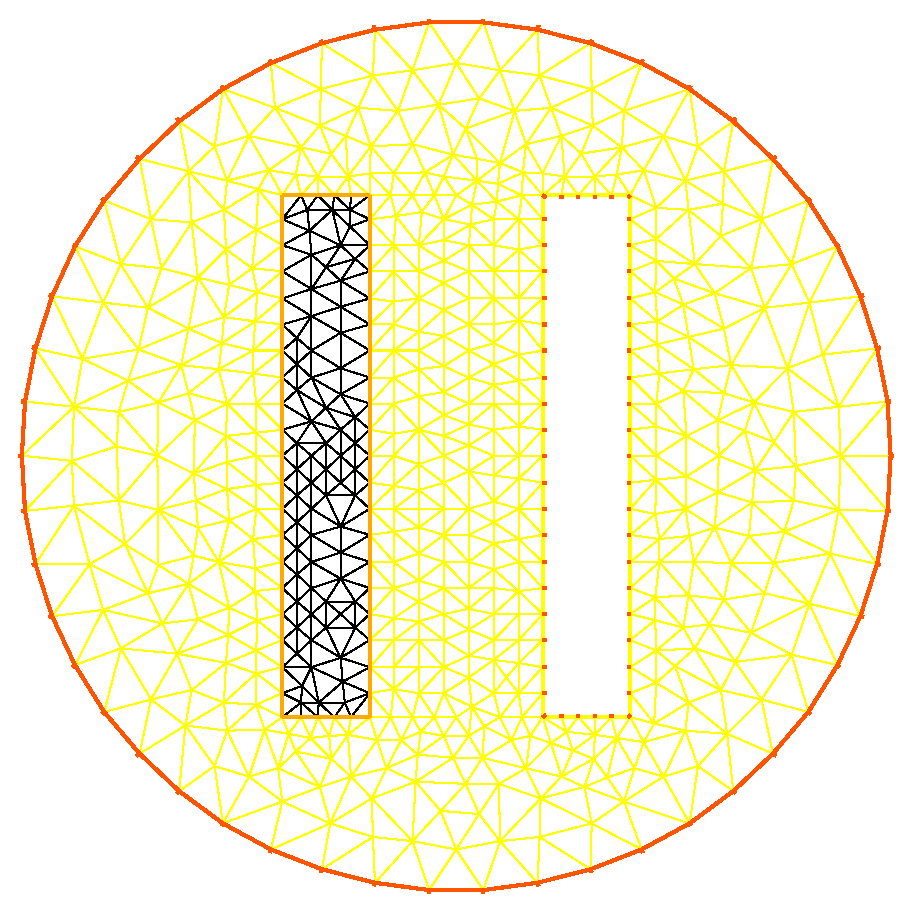
\includegraphics[width=6cm]{heatexTh}~~~
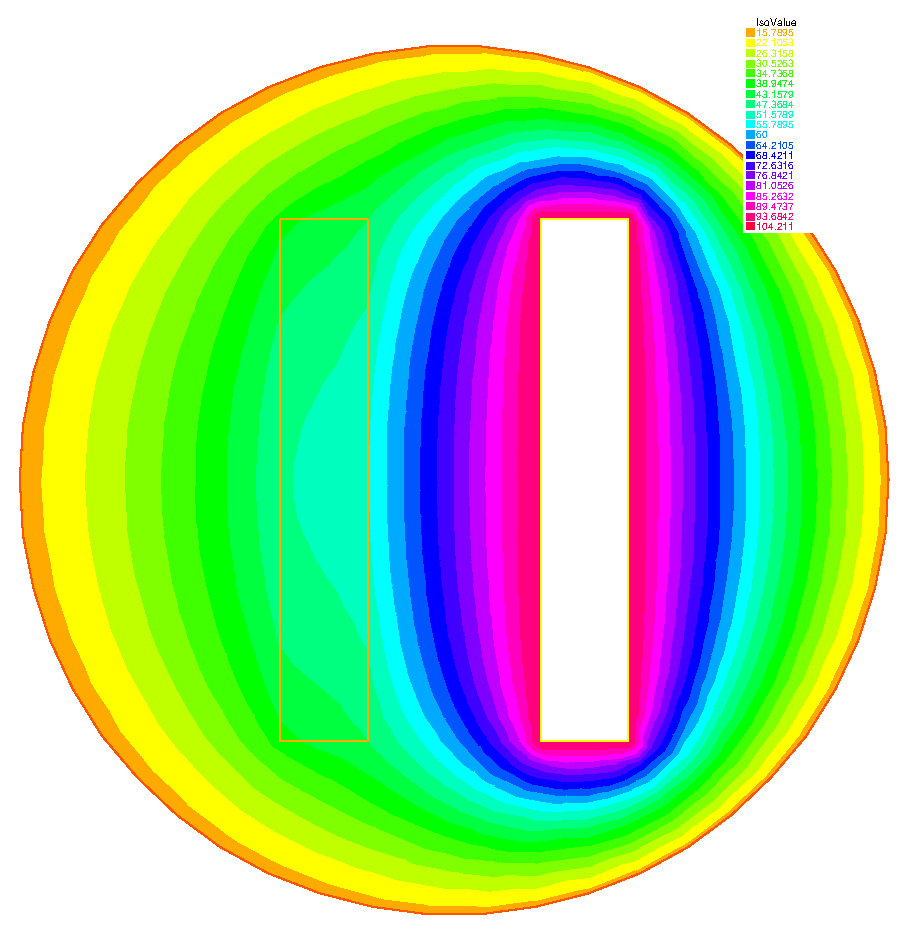
\includegraphics[width=6cm]{heatex}
\caption{ The heat exchanger}
\end{center}
\end{figure}

\paragraph{Exercise} Use the symmetry of the problem with respect to the axes;
triangulate only one quarter of the domain, and set \x{Dirichlet}
conditions on the vertical axis, and Neumann conditions on the
horizontal axis.%\fin

\bigskip

\paragraph{Writing and reading triangulation files}
Suppose that at then end of the previous program we had added the line
\bFF
savemesh(Th,"condensor.msh");
\eFF
and then later on we write a similar program but we wish to read the mesh from that
file. Then this is how the condenser should be computed:
\bFF
@mesh Sh=@readmesh("condensor.msh");
fespace Wh(Sh,P1); Wh us,vs;
@solve b(us,vs)= @int2d(Sh)(@dx(us)*@dx(vs)+@dy(us)*@dy(vs))
                +@on(1,us=0)+@on(99,us=1)+@on(98,us=-1);
@plot(us);
\eFF
Note that the name of the boundary are lost but either its internal number
(in the case of C0) or its label number (for C1 and C2) are kept.


 \subsection{Acoustics}

\paragraph{Summary}
\emph{Here we come to grip with \x{ill posed problems} and \x{eigen value problems}}

Pressure variations in air at rest are governed by the wave equation:
\[
     {\p^2 u \over \p t^2} - c^2 \Delta u =0.
\]
When the solution wave is monochromatic (and that depend on the boundary and initial conditions)
, $u$ is of the form
$u(x,t)=Re(v(x) e^{ik t})$ where $v$ is a solution of Helmholtz's equation:
%
\begin{eqnarray}&&
 k ^{2}v  + c^{2}\Delta v  =0 ~\hbox{~in~}~~\Omega,
 \cr&&
 \frac{\p v}{\p n}|_\Gamma=g.
\end{eqnarray}
%
where $g$ is the source.
Note the ``+'' sign in front of the Laplace operator. This sign may make the
problem ill posed for some values of $\frac c k$, a phenomenon called
 ``resonance''.\\
At resonance there are non-zero solutions even when $g=0$. So the following program may or may not work:

\begin{example}[sound.edp]
\bFF
// file sound.edp
@real kc2=1;
@func g=y*(1-y);

@border a0(t=0,1) { x= 5; y= 1+2*t ;}
@border a1(t=0,1) { x=5-2*t; y= 3 ;}
@border a2(t=0,1) { x= 3-2*t; y=3-2*t ;}
@border a3(t=0,1) { x= 1-t; y= 1 ;}
@border a4(t=0,1) { x= 0; y= 1-t ;}
@border a5(t=0,1) { x= t; y= 0  ;}
@border a6(t=0,1) { x= 1+4*t; y= t ;}

@mesh Th=@buildmesh( a0(20) + a1(20) + a2(20)
        + a3(20) + a4(20) + a5(20) + a6(20));
@fespace Vh(Th,P1);  Vh u,v;

solve sound(u,v)=@int2d(Th)(u*v * kc2 - @dx(u)*@dx(v) - @dy(u)*@dy(v))
                 - @int1d(Th,a4)(g*v);
@plot(u, wait=1, ps="sound.eps");
\eFF
\end{example}

Results are on Figure \ref{figsound}.  But when $kc2$ is an eigen value of the problem, then the
solution not unique: $u_e$ the eigen state, "u" a solution $\Rightarrow$ $u+u_e$ is also a solution.
To find all the $u_e$ one can do the following
\bFF
@real sigma = 20;  // value of the shift
// OP = A - sigma B ;  //  the shifted matrix
@varf  op(u1,u2)= @int2d(Th)(  @dx(u1)*@dx(u2) + @dy(u1)*@dy(u2) - sigma* u1*u2 );
@varf b([u1],[u2]) = @int2d(Th)(  u1*u2 ) ; // no  Boundary condition

@matrix OP= op(Vh,Vh,solver=Crout,factorize=1);
@matrix B= b(Vh,Vh,solver=CG,eps=1e-20);

@int nev=2;  // number of requested eigen values near sigma

@real[int] ev(nev); // to store the  nev eigenvalue
Vh[int] eV(nev);   // to store the nev eigenvector

@int k=EigenValue(OP,B,sym=true,sigma=sigma,value=ev,vector=eV,
                   tol=1e-10,maxit=0,ncv=0);
@cout<<ev(0)<<" 2 eigen values "<<ev(1)<<endl;
v=eV[0];
@plot(v,wait=1,ps="eigen.eps");
\eFF
\begin{figure}[htbp]
\begin{center}\label{figsound}
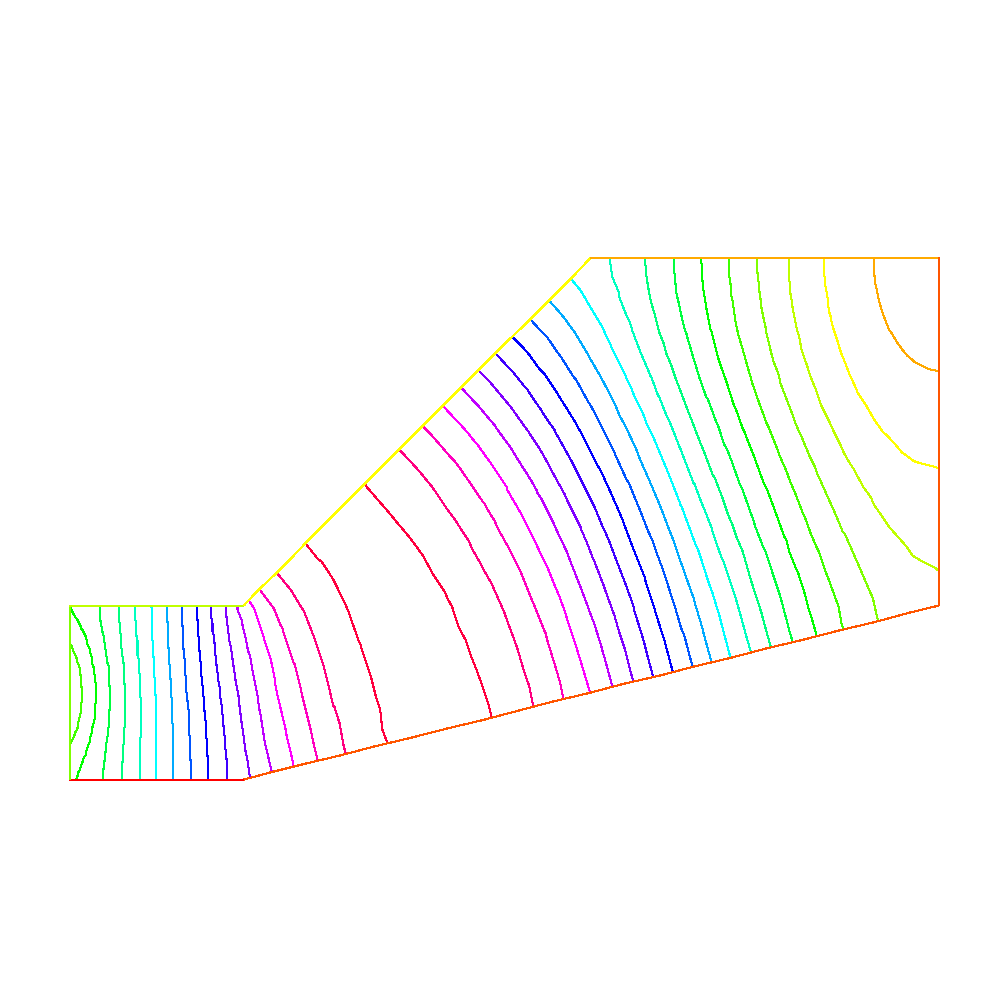
\includegraphics[width=8cm]{sound0}~~~
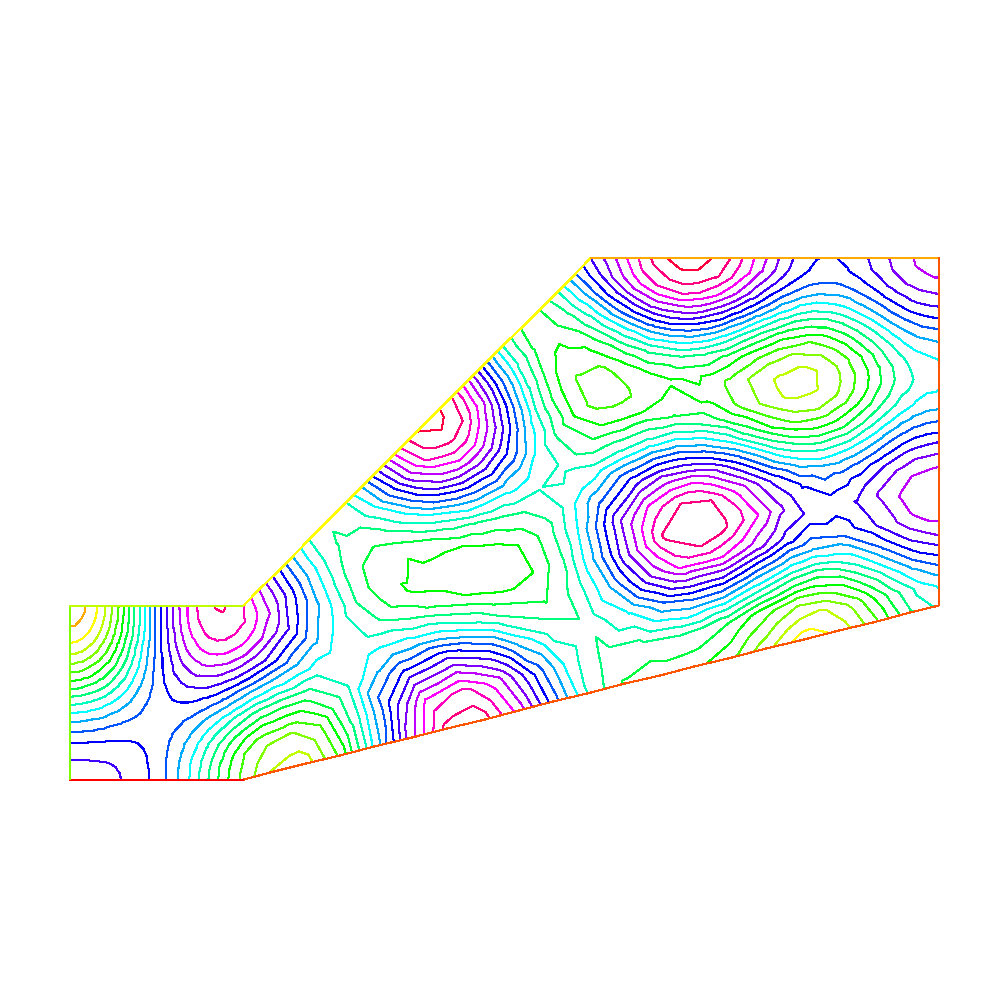
\includegraphics[width=8cm]{eigen}

\caption{Amplitude of an acoustic signal coming from the left vertical wall.
Right:  first eigen state ($(k/c)^2=19.4256$)}
\end{center}
\end{figure}

\subsection{Thermal Conduction}

\paragraph{Summary}\emph{ Here we shall learn how to deal with a \x{
time dependent} \x{Parabolic} problem. We shall also show how to treat a
\x{axisymmetric} problem  and show also how to deal with a \x{nonlinear problem}.}

\paragraph{How air cools a plate}

We seek the temperature distribution in a plate $(0,Lx)\times(0,Ly)\times(0,Lz)$
of rectangular cross section $\Omega=(0,6)\times(0,1)$; the plate is
surrounded by air at temperature $u_e$ and
initially at temperature $u=u_0+\frac x L u_1$. In the plane perpendicular to the plate
at $z=Lz/2$,  the temperature varies little with
the coordinate z; as a first approximation the problem is 2D.
\\\\
We must solve the temperature equation in $\Omega$ in a time interval (0,T).
\begin{eqnarray}&&
    \p_t u -\n\cdot(\kappa\n u)=0 \hbox{ in } \Omega\times(0,T),
    \cr&&
    u(x,y,0)=u_0+x u_1
    \cr&&
    \kappa\frac{\p u}{\p n} +\alpha(u-u_e)=0\hbox{ on } \Gamma\times(0,T).
\end{eqnarray}
Here the diffusion $\kappa$ will take two values, one below the middle horizontal line and ten times less
above, so as to simulate a thermostat.
The term $\alpha(u-u_e)$ accounts for the loos of temperature by convection in air.  Mathematically
this boundary condition is of \x{Fourier} (or \x{Robin}, or \x{mixed}) type.
\\
The variational formulation is $L^2(0,T;H^(\Omega))$; in loose terms and after applying an implicit Euler
finite difference approximation in time; we shall seek for $u^n(x,y)$ satisfying for all $w\in H^1(\Omega)$:
\[
    \int_\Omega(\frac{u^n-u^{n-1}}{\delta t} w + \kappa\n u^n\n w) +\int_\Gamma\alpha(u^n-u_ue)w=0
\]
\bFF
@func u0 =10+90*x/6;
@func k = 1.8*(y<0.5)+0.2;
@real ue = 25, alpha=0.25, T=5, dt=0.1 ;

@mesh Th=@square(30,5,[6*x,y]);
@fespace Vh(Th,P1); Vh u=u0,v,uold;

@problem thermic(u,v)= @int2d(Th)(u*v/dt + k*(@dx(u) * @dx(v) + @dy(u) * @dy(v)))
                + @int1d(Th,1,3)(alpha*u*v)
                - @int1d(Th,1,3)(alpha*ue*v)
                - @int2d(Th)(uold*v/dt) + @on(2,4,u=u0);
@ofstream ff("thermic.dat");
@for(@real t=0;t<T;t+=dt){
    uold=u;
    thermic;
    ff<<u(3,0.5)<<@endl;
    @plot(u);
}
\eFF
Notice that we must separate by hand the bilinear part from the linear one.

Notice also the way we store the temperature at point (3,0.5) for all times in file {\tt thermic.dat"}.
Should a one dimensional plot be required, the same procedure can be used.  For instance to
print $x\to\frac{\p u}{\p y}(x,0.9)$ one would do
\bFF
@for(@int i=0;i<20;i++) @cout<<@dy(u)(6.0*i/20.0,0.9)<<@endl;
\eFF
Results are shown on Figure \ref{figthermic}.

\begin{figure}[htbp]
\begin{center}\label{figthermic}
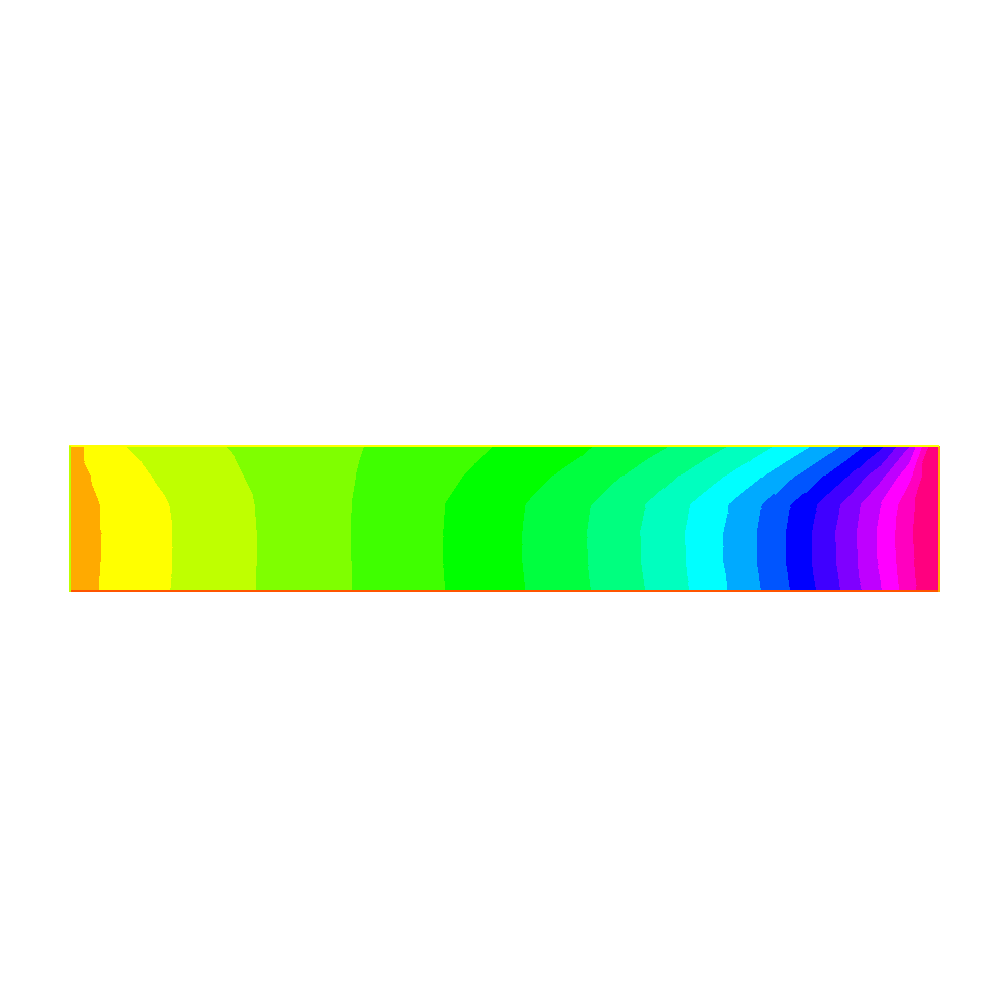
\includegraphics[width=8cm]{thermic}~~~
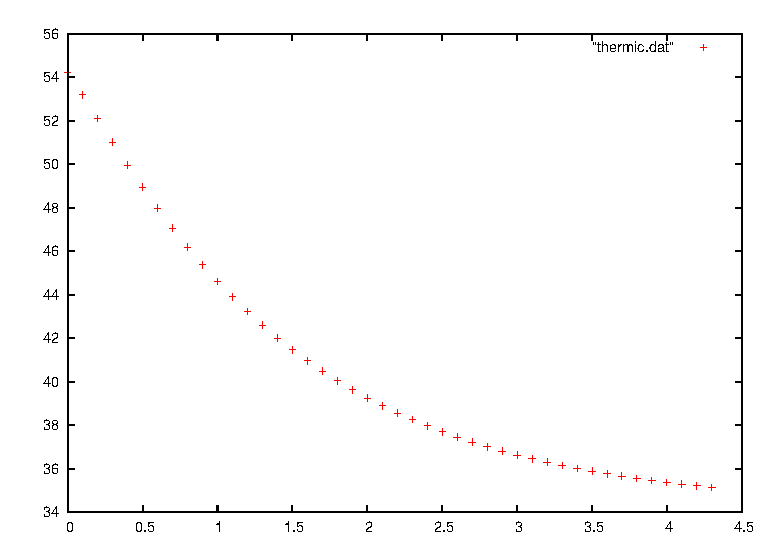
\includegraphics[width=8cm]{thermicvst}

\caption{ Temperature at T=4.9. Right: decay of temperature versus time at x=3, y=0.5}
\end{center}
\end{figure}

\subsubsection{Axisymmetry: 3D Rod with circular section}

Let us now deal with a cylindrical rod instead of a flat plate.  For simplicity we take $\kappa=1$.
In cylindrical coordinates, the Laplace
operator becomes ($r$ is distance to the axis, $z$ distance along the
axis, $\theta$ polar angle in a fixed plane perpendicular to the axis):

$$ \Delta u = {1\over r}\p _r(r\p _r u) + {1\over r^2}\p ^2_{\theta\theta} u
 + \p ^2_{z z}.
$$

Symmetry implies that we loose the dependence with respect to
$\theta$; so the domain $\Omega$ is again a rectangle. We take the convention of
numbering of the edges as in {\tt square()} (1 for the bottom horizontal ...);
the problem is now:

\begin{eqnarray}&&
r\p_t u-\p _r(r\p _r u) - \p _z(r\p _z u) = 0 \hbox{ in } \Omega,
\cr&&
u(t=0) = u_0 + \frac z{L_z} (u_1-u_)
\cr&&
u|_{\Gamma_4} = u_0,\quad  u|_{\Gamma_2} = u_1,
\quad \alpha(u-u_e) + {\p u\over \p n} |_{\Gamma_1\cup\Gamma_3} = 0.
\end{eqnarray}
Note that the PDE has been multiplied by $r$.

Now in the \freefempp syntax $r$ becomes $x$ and $z$ becomes $y$ and the problem is:
\bFF
@problem thermaxi(u,v)=@int2d(Th)((u*v/dt + @dx(u)*@dx(v) + @dy(u)*@dy(v))*x)
                + @int1d(Th,3)(alpha*x*u*v) - @int1d(Th,3)(alpha*x*ue*v)
                - @int2d(Th)(uold*v*x/dt) + @on(2,4,u=u0);
\eFF
Notice that the bilinear form degenerates at $x=0$. Still one can prove existence and uniqueness
for $u$ and because of this degeneracy no boundary conditions need be imposed on $\Gamma_1$.

\subsubsection{A Nonlinear Problem : Radiation}

Heat loss through \x{radiation}  is a loss proportional
to the absolute temperature to the fourth power. This adds to the
loss by convection and gives the following
boundary condition:
 $$\kappa{\p u\over \p n} +\alpha(u-u_e) + c[(u + 273)^4 - (u_e+273)^4] = 0$$

The problem is \x{nonlinear}, and must be solved iteratively. If $m$
denotes the iteration index, a semi-linearization of the radiation condition gives
$${\p u^{m+1}\over \p n} + \alpha(u^{m+1}-u_e)+ c(u^{m+1}-u_e)
(u^m+u_e +546) ((u^m + 273)^2 + (u_e+273)^2)  = 0,
$$
because we have the identity
$ a^4 - b^4 = (a-b)(a+b)(a^2+b^2)$.
The iterative process will work with $v=u-u_e$.
\bFF
...
@fespace Vh(Th,P1);
@real rad=1e-8, uek=ue+273;
Vh vold,w,v=u0-ue,b;
@problem thermradia(v,w)
    = @int2d(Th)(v*w/dt + k*(@dx(v) * @dx(w) + @dy(v) * @dy(w)))
                + @int1d(Th,1,3)(b*v*w)
                - @int2d(Th)(vold*w/dt) + @on(2,4,v=u0-ue);

@for(@real t=0;t<T;t+=dt){
    vold=v;
    @for(@int m=0;m<5;m++){
       b= alpha + rad * (v + 2*uek) * ((v+uek)^2 + uek^2);
       thermradia;
    }
}
vold=v+ue; @plot(vold);
\eFF


\subsection{Irrotational Fan Blade Flow and Thermal effects}

\paragraph{Summary}\emph{Here we will learn how to deal with a \x{multi-physics system}
of PDEs on a \x{Complex geometry,} with \x{multiple meshes} within one problem.  We
also learn how to manipulate the \x{region indicator} and see how smooth is the projection
operator from one mesh to another.}

 \paragraph{Incompressible flow}

Without viscosity and vorticity incompressible flows have a velocity given by:
 $$
 u=\begin{matrix}{\p \psi \over \p x_{2} }, -{\p \psi
 \over \p x_{1}} \end{matrix}
  \hbox{,  where $\psi  $ is solution of }  \Delta \psi =0
$$
This equation expresses both incompressibility
 ($\nabla\cdot u=0$) and absence of vortex ($\nabla\times u =0$).

As the fluid slips along the walls, normal velocity is zero, which
means that $\psi$ satisfies:
$$
 \psi \hbox{ constant on the walls}.
$$
One can also prescribe the normal velocity at an artificial boundary, and this translates into
 non constant {Dirichlet} data for $\psi$.
\\\\

\paragraph{Airfoil}

Let us consider a wing profile $S$ in a uniform flow. Infinity will be
represented by a large circle  $C$ where the flow is assumed to be of uniform velocity;
one way to model this problem is to write
 \begin{eqnarray}&&
 \Delta \psi =0 ~\hbox{~in~}~ \Omega, \qquad
 \psi |_{S}=0, \quad
 \psi|_{C}= {u_\infty}y,
\end{eqnarray}
 where $\partial\Omega=C\cup S $

\paragraph{The NACA0012 Airfoil}
An equation for the upper surface of a NACA0012 (this is a classical
  wing profile in aerodynamics) is:
$$    y = 0.17735\sqrt{x}-0.075597x- 0.212836x^2+0.17363x^3-0.06254x^4.$$
%
\begin{example}[potential.edp]
\bFF
// file potential.edp

@real S=99;
@border C(t=0,2*pi) {  x=5*cos(t);  y=5*sin(t);}
@border Splus(t=0,1){  x = t; y = 0.17735*sqrt(t)-0.075597*t
        - 0.212836*(t^2)+0.17363*(t^3)-0.06254*(t^4); label=S;}
@border Sminus(t=1,0){  x =t; y= -(0.17735*sqrt(t)-0.075597*t
        -0.212836*(t^2)+0.17363*(t^3)-0.06254*(t^4)); label=S;}
@mesh Th= @buildmesh(C(50)+Splus(70)+Sminus(70));
@fespace Vh(Th,P2); Vh psi,w;

@solve potential(psi,w)=@int2d(Th)(@dx(psi)*@dx(w)+@dy(psi)*@dy(w))+
  @on(C,psi = y) + @on(S,psi=0);

@plot(psi,wait=1);

\eFF
\end{example}

A zoom of the streamlines are shown on Figure \ref{figpotential}.

\begin{figure}[htbp]
\begin{center}\label{figpotential}
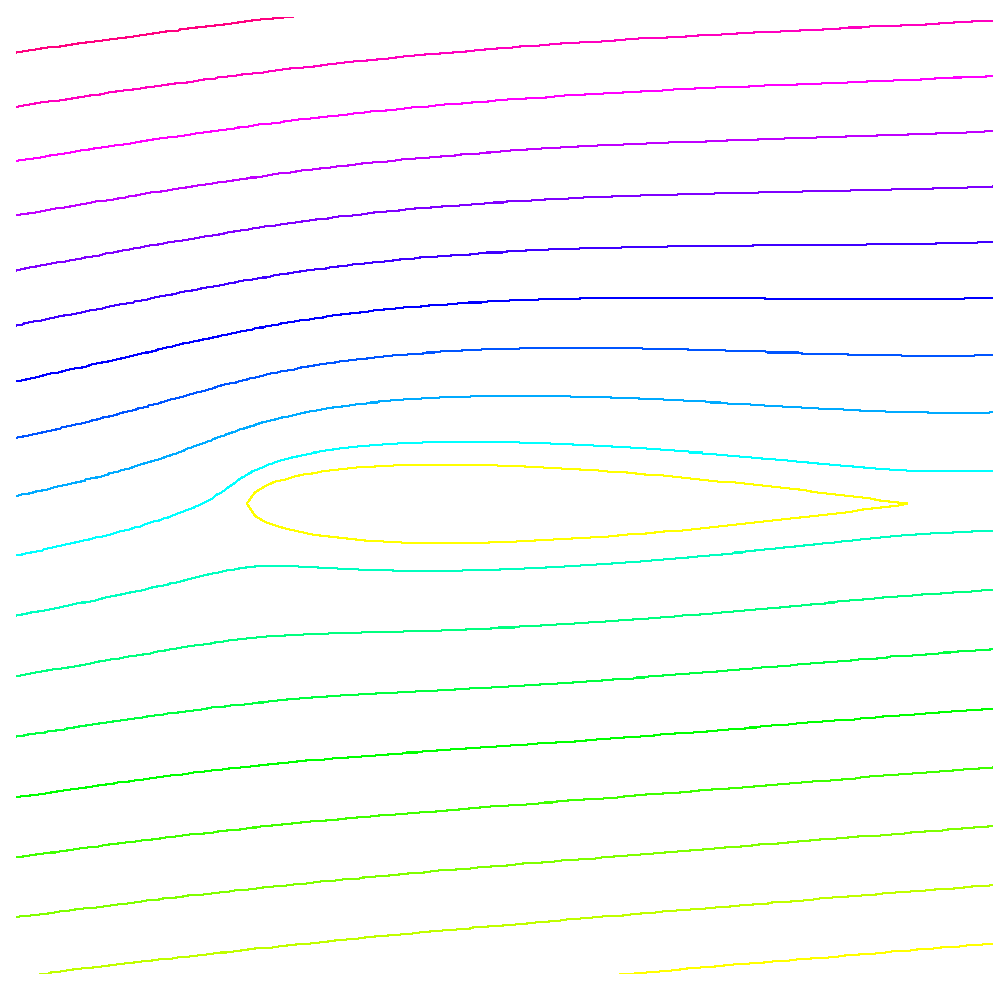
\includegraphics[width=8cm]{potential}
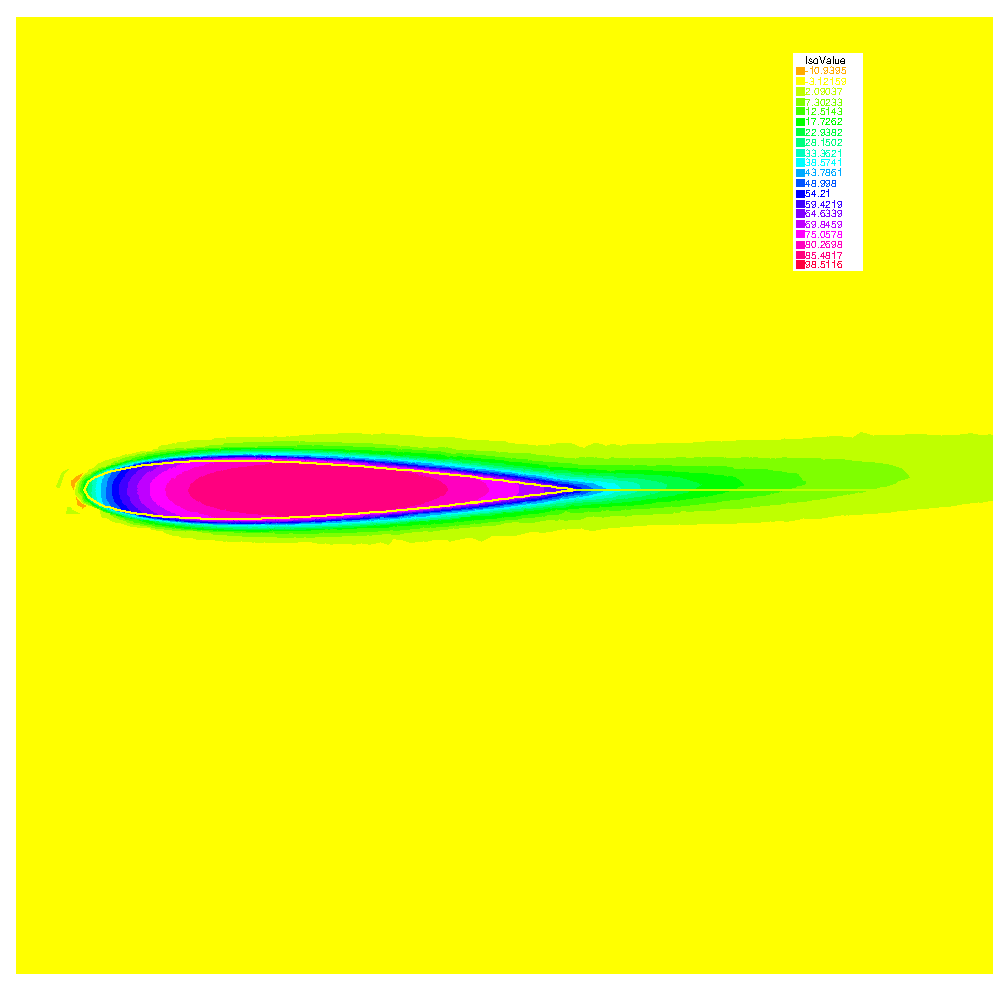
\includegraphics[width=8cm]{potheat}

\caption{ Zoom around the NACA0012 airfoil showing the streamlines (curve $\psi=$ constant).
To obtain such a plot use the interactive graphic command: ``+" and p.
Right: temperature distribution at time T=25 (now the maximum is at 90 instead of 120).
Note that an incidence angle has been added here (see Chapter 9).}
\end{center}
\end{figure}

 \subsubsection{Heat Convection around the airfoil}
Now let us assume that the airfoil is hot and that air is there to cool it.
Much like in the previous section the heat equation for the temperature $u$ is
$$
\p_t v -\n\cdot(\kappa\n v) + u\cdot\n v =0,~~v(t=0)=v_0, ~~\frac{\p v}{\p n}|_C=0
$$
But now the domain is outside AND inside $S$ and $\kappa$ takes a different value in air
and in steel.  Furthermore there is convection of heat by the flow, hence the
term $u\cdot\n v$ above.  Consider the following, to be plugged at the end of the previous program:
\bFF
...
@border D(t=0,2){x=1+t;y=0;} // added to have a fine mesh at trail
@mesh Sh = @buildmesh(C(25)+Splus(-90)+Sminus(-90)+D(200));
@fespace Wh(Sh,P1); Wh v,vv;
@int steel=Sh(0.5,0).region, air=Sh(-1,0).region;
@fespace W0(Sh,P0);
W0 k=0.01*(@region==air)+0.1*(@region==steel);
W0 u1=dy(psi)*(@region==air), u2=-@dx(psi)*(@region==air);
Wh vold = 120*(@region==steel);
@real dt=0.05, nbT=50;
@int i;
@problem thermic(v,vv,init=i,solver=LU)= @int2d(Sh)(v*vv/dt
                + k*(@dx(v) * @dx(vv) + @dy(v) * @dy(vv))
                + 10*(u1*@dx(v)+u2*@dy(v))*vv)- @int2d(Sh)(vold*vv/dt);
@for(i=0;i<nbT;i++){
    v=vold; thermic;
 @plot(v);
}
\eFF
Notice here
\begin{itemize}
\item how steel and air are identified by the mesh parameter region which is defined when buildmesh is
called and takes an integer value corresponding to each connected component of $\Omega$;

\item how the convection terms are added without upwinding. Upwinding is necessary when the
Pecley number $|u|L/\kappa$ is large (here is a typical length scale), The factor 10 in front of
the convection terms is a quick way of multiplying the velocity by 10 (else it is too slow to see something).

\item The solver is Gauss' LU factorization and when {\tt init}$\neq 0$ the LU decomposition is reused so it
is much faster after the first iteration.
\end{itemize}

\subsection{Pure Convection : The Rotating Hill}

\paragraph{Summary}\emph{ Here we will present two methods for \x{upwinding} for the simplest
convection problem.  We will learn about \x{Characteristics-Galerkin}
and \x{Discontinuous-Galerkin} Finite Element Methods.}

Let $\Omega$ be the unit disk centered at 0; consider the rotation vector field
$$ u_1 = y,\quad u_2 = -x.$$
Pure convection by $u$ is
$$
    \p_t c  + u.\nabla c  = 0~\hbox{~in~}~~\Omega\times(0,T)
    ~~~ c (t=0) =  c ^0~\hbox{~in~}~~\Omega.
$$
The exact solution is  $ c (x,y,t) =  c ^0(X(0),Y(0))$ where $\vec X:=(X,Y)$
are solutions of ($\vec u =(u_1,u_2$)
\[
    \frac{\d\vec X}{\d\tau} = u(\vec X,\tau),~~~\vec X(t)=(x,y).
\]

The game consists in solving the equation until $T=2\pi$, that is for
a full revolution and to compare the final solution with the initial one;
they should be equal.

\paragraph{Solution by a Characteristics-Galerkin Method}
In \freefempp there is an operator called {\tt convect([u1,u2],dt,c)} which solves
exactly the equation for ${\vec X}^m:=(X(t),Y(t))$ at $t=m\delta t$:
\[
    \frac\d{\d\vec X}{\tau}(X,Y) = u(\vec X,\tau),~~~\vec X(t-\d t)=(x,y).
\]

When $u$ is piecewise constant; this is possible because
$(X,Y)$ is then a polygonal curve which can be computed exactly and the solution exists always when
$u$ is divergence free; convect returns  $c(\vec X^m,t-\d t)$.

\begin{example}[convects.edp]
\bFF
// file convects.edp

@border C(t=0, 2*pi) { x=cos(t);  y=sin(t); };
@mesh Th = @buildmesh(C(100));
@fespace Uh(Th,P1);
Uh cold, c = exp(-10*((x-0.3)^2 +(y-0.3)^2));

@real dt = 0.17,t=0;
Uh u1 = y, u2 = -x;
@for (int m=0; m<2*pi/dt ; m++) {
    t += dt;     cold=c;
    c=@convect([u1,u2],-dt,cold);
    @plot(c,cmm=" t="+t + ", min=" + c[].min + ", max=" +  c[].max);
}

\eFF
\end{example}

The method is very powerful but has two limitations: a/ it is not conservative, b/ it may diverge
in rare cases when $|u|$ is too small due to quadrature error.

\paragraph{Solution by Discontinuous-Galerkin FEM}

Discontinuous Galerkin methods take advantage of the discontinuities of $c$ at the edges to build
upwinding.  There are may formulations possible. We shall implement here the so-called dual-$P^1_{DC}$
formulation (see Ern\cite{ern}):
\[
    \int_\Omega(\frac{c^{n+1}-c^n}{\delta t} +u\cdot\n c)w
    +\int_E(\alpha|n\cdot u|-\frac 12 n\cdot u)[c]w
    =\int_{E_\Gamma^-}|n\cdot u| cw~~~\forall w
\]
where $E$ is the set of inner edges and $E_\Gamma^-$ is the set of boundary edges where $u\cdot n<0$
(in our case there is no such edges). Finally $[c]$ is the jump of $c$ across an edge with the convention
that $c^+$ refers to the value on the right of the oriented edge.
\begin{example}[convects\_end.edp]
\bFF
// file convects.edp
...
@fespace Vh(Th,P1dc);

Vh w, ccold, v1 = y, v2 = -x, cc = exp(-10*((x-0.3)^2 +(y-0.3)^2));
@real u, al=0.5;  dt = 0.05;

@macro n(N.x*v1+N.y*v2) // @problem  Adual(cc,w) =
@int2d(Th)((cc/dt+(v1*@dx(cc)+v2*@dy(cc)))*w)
  + @intalledges(Th)((1-@nTonEdge)*w*(al*abs(n)-n/2)*@jump(cc))
//  - @int1d(Th,C)((n<0)*abs(n)*cc*w)  // unused because cc=0 on $\p\Omega^-$
  - @int2d(Th)(ccold*w/dt);

for ( t=0; t< 2*pi ; t+=dt)
{
  ccold=cc; Adual;
  @plot(cc,fill=1,cmm="t="+t + ", min=" + cc[].min + ", max=" +  cc[].max);
};
@real [int] viso=[-0.2,-0.1,0,0.1,0.2,0.3,0.4,0.5,0.6,0.7,0.8,0.9,1,1.1];
@plot(c,wait=1,fill=1,ps="convectCG.eps",viso=viso);
@plot(c,wait=1,fill=1,ps="convectDG.eps",viso=viso);

\eFF
\end{example}
Notice the new keywords, \x{intalledges} to integrate on all edges, \x{nTonEdge} which is one
if the triangle has a boundary edge and zero otherwise, {\tt jump} to implement $[c]$.
Results of both methods are shown on Figure \ref{figconvect} with identical levels for the \x{level line};
this is done with the plot-modifier \x{viso}.

Notice also the  \x{macro} where the parameter $u$ is not used (but
the syntax needs one) and which ends with a //; it simply replaces
the name {\tt n} by {\tt (N.x*v1+N.y*v2)}. As easily guessed {\tt
N.x,N.y} is the \x{normal} to the edge.

\begin{figure}[htbp]
\begin{center}\label{figconvect}
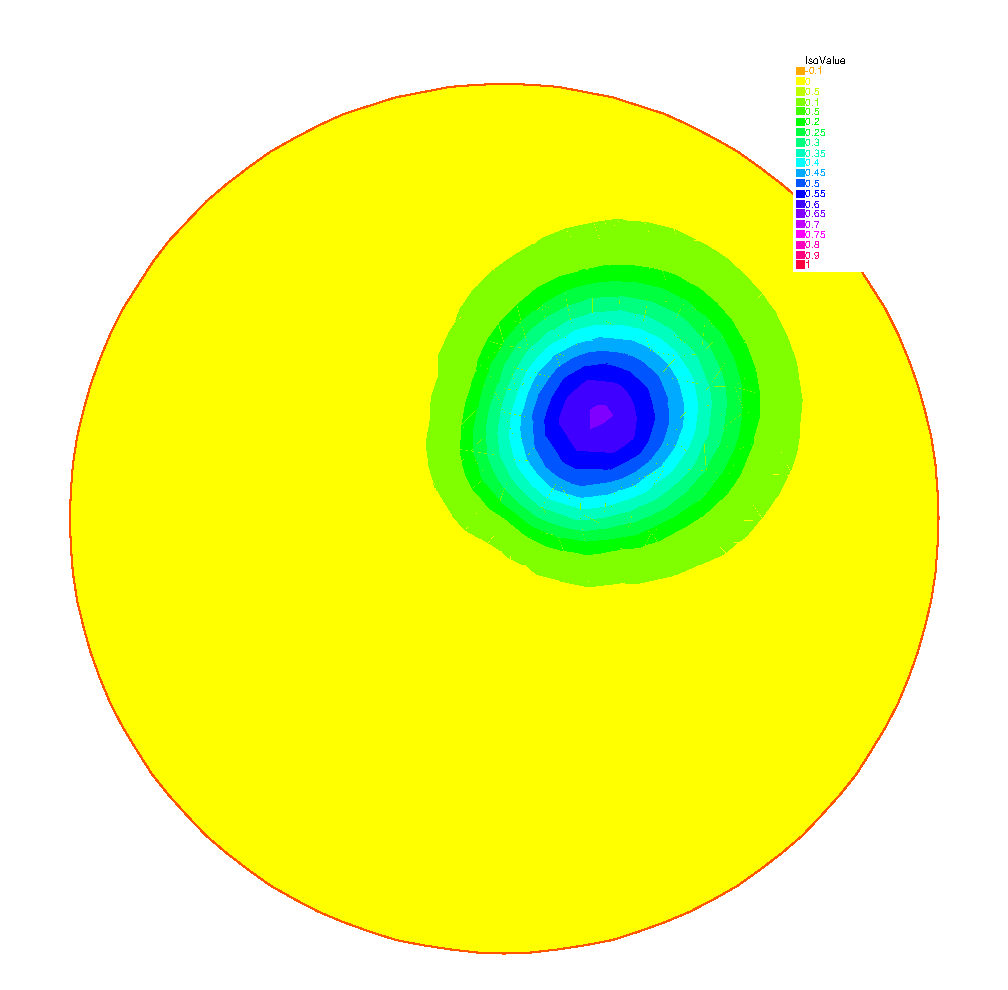
\includegraphics[width=8cm]{convectCG}
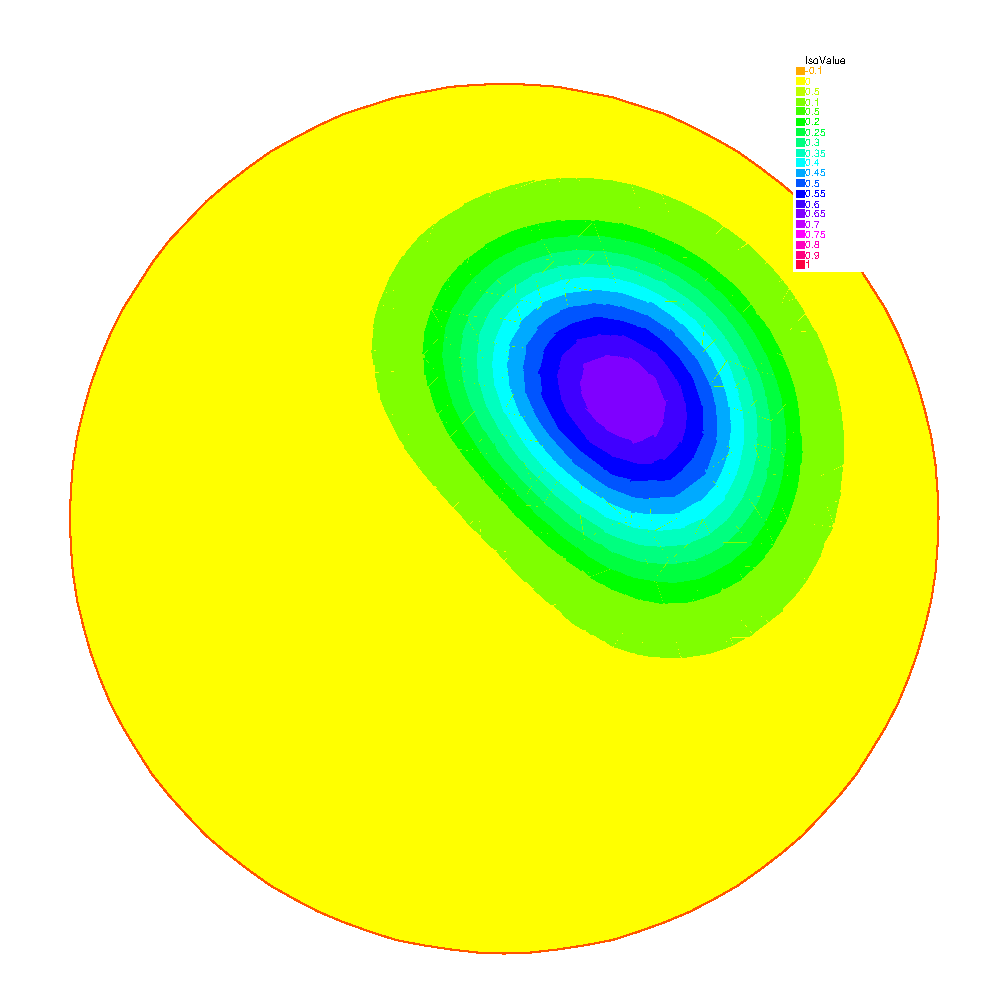
\includegraphics[width=8cm]{convectDG}

\caption{ The rotated hill after one revolution, left with Characteristics-Galerkin,
on the right with Discontinuous $P^1$ Galerkin FEM.}
\end{center}
\end{figure}

Now if you think that DG is too slow try this
\bFF

// the same DG very much faster
@varf aadual(cc,w) = @int2d(Th)((cc/dt+(v1*@dx(cc)+v2*@dy(cc)))*w)
        + @intalledges(Th)((1-@nTonEdge)*w*(al*abs(n)-n/2)*@jump(cc));
@varf bbdual(ccold,w) =  - @int2d(Th)(ccold*w/dt);
@matrix  AA= aadual(Vh,Vh);
@matrix BB = bbdual(Vh,Vh);
@set (AA,init=t,solver=UMFPACK);
Vh rhs=0;
@for ( t=0; t< 2*pi ; t+=dt)
{
  ccold=cc;
  rhs[] = BB* ccold[];
  cc[] = AA^-1*rhs[];
  @plot(cc,fill=0,cmm="t="+t + ", min=" + cc[].min + ", max=" +  cc[].max);
};
\eFF
Notice the new keyword \x{set} to specify a solver in this framework; the modifier \x{init} is used
to tel the solver that the matrix has not changed (init=true).

\paragraph{\x{Finite Volume Methods}} can also be handled with \freefempp but it requires programming.
For instance the $P^0-P^1$ Finite Volume Method of Dervieux et al associates to each $P^1$
function $c^1$ a $P^0$ function $c^0$ with constant value around each vertex $q^i$ equal to $c^1(q^i)$
on the cell $\sigma_i$ made by all the medians of all triangles having $q^i$ as vertex.
Then upwinding is done by taking left or right values at the median:
\[
    \int_{\sigma_i}\frac 1{\delta t}({c^1}^{n+1}-{c^1}^n) + \int_{\p\sigma_i}u\cdot n c^-=0
    ~~~\forall i
\]
It can be programmed as
\bFF
@load "mat_dervieux";  // external module in C++ must be loaded
@border a(t=0, 2*pi){ x = cos(t); y = sin(t);  }
@mesh th = @buildmesh(a(100));
@fespace Vh(th,P1);

Vh vh,vold,u1 = y, u2 = -x;
Vh v = exp(-10*((x-0.3)^2 +(y-0.3)^2)), vWall=0, rhs =0;

@real dt = 0.025;
// qf1pTlump means mass lumping is used
@problem  FVM(v,vh) = @int2d(th,qft=qf1pTlump)(v*vh/dt)
                  - @int2d(th,qft=qf1pTlump)(vold*vh/dt)
      + @int1d(th,a)(((u1*N.x+u2*N.y)<0)*(u1*N.x+u2*N.y)*vWall*vh)
+ rhs[] ;

@matrix A;
MatUpWind0(A,th,vold,[u1,u2]);

@for ( @int t=0; t< 2*pi ; t+=dt){
  vold=v;
  rhs[] = A * vold[] ; FVM;
  @plot(v,wait=0);
};
\eFF
the \x{mass lumping} parameter forces a quadrature formula with Gauss points at the vertices
so as to make the mass matrix diagonal; the linear system solved by a conjugate gradient method for
instance will then converge in one or two iterations.

The right hand side {\tt rhs} is computed by an \x{external C++ function} {\tt MatUpWind0(...)}
which is programmed as
\bFF
// computes matrix a on a triangle for the Dervieux FVM
@int   fvmP1P0(@double q[3][2], // the 3 vertices of a triangle T
              @double u[2],   // convection velocity on T
              @double c[3],   // the P1 function on T
              @double a[3][3],// output matrix
              @double where[3] ) // where>0 means we're on the boundary
{
  @for(@int i=0;i<3;i++) @for(@int j=0;j<3;j++) a[i][j]=0;

    @for(@int i=0;i<3;i++){
        @int ip = (i+1)%3, ipp =(ip+1)%3;
        @double unL =-((q[ip][1]+q[i][1]-2*q[ipp][1])*u[0]
                    -(q[ip][0]+q[i][0]-2*q[ipp][0])*u[1])/6;
        @if(unL>0) { a[i][i] += unL; a[ip][i]-=unL;}
            @else{ a[i][ip] += unL; a[ip][ip]-=unL;}
        @if(where[i]&&where[ip]){        // this is a boundary edge
            unL=((q[ip][1]-q[i][1])*u[0] -(q[ip][0]-q[i][0])*u[1])/2;
            if(unL>0) { a[i][i]+=unL; a[ip][ip]+=unL;}
        }
    }
  return 1;
}
\eFF
It must be inserted into a larger .cpp file, shown in Appendix A,
 which is the load module linked to \freefempp.

\subsection{A Projection Algorithm for the Navier-Stokes equations }
\paragraph{Summary}\emph{Fluid flows require good algorithms and good triangultions. We show
here an example of a complex algorithm and or first example of \x{mesh adaptation}}.
\\\\
An incompressible viscous fluid satisfies:
$$ \p _t u + u\cdot\nabla u + \nabla p - \nu\Delta u = 0,\quad  \nabla\cdot u=0
\quad  \hbox{ in } \Omega\times ]0,T[,
$$
$$ u|_{t=0} = u^0,\quad  u|_\Gamma = u_\Gamma.
$$
A possible algorithm, proposed by Chorin, is
$$ {1\over \delta t}[u^{m+1} - u^moX^m] + \nabla p^m -\nu\Delta u^m= 0,\quad  u|_\Gamma
 = u_\Gamma,
 $$
$$ -\Delta p^{m+1} = -\nabla\cdot  u^moX^m, \quad  \p _n p^{m+1} = 0,
$$
where $uoX(x) = u(x-u(x)\delta t)$ since $\p _t u + u\cdot\nabla
u $ is approximated by the method of characteristics, as in the previous section.
\\\\
An improvement over Chorin's algorithm, given by Rannacher, is to compute a correction, q,
to the pressure (the overline denotes the mean over $\Omega$)
\[
    -\Delta q= \n\cdot\vec u - \overline{\n\cdot\vec u}
\]
and define
\[
    u^{m+1}=\tilde u + \n q\delta t,~~~p^{m+1}=p^m-q-\overline{p^m-q}
\]
where $\tilde u$ is the $(u^{m+1},v^{m+1})$ of Chorin's algorithm.

\paragraph{The backward facing step}

The geometry is that of a channel with a backward facing step so that
the inflow section is smaller than the outflow section. This geometry
produces a fluid recirculation zone that must be captured correctly.

This can only be done if the triangulation is sufficiently fine, or
well adapted to the flow.

\begin{example}[NSprojection.edp]
\bFF
// file NSprojection.edp

@border a0(t=1,0){ x=0;      y=t;           @label=1;}
@border a1(t=0,1){ x=2*t;    y=0;           @label=2;}
@border a2(t=0,1){ x=2;      y=-t/2;        @label=2;}
@border a3(t=0,1){ x=2+18*t^1.2;  y=-0.5;   @label=2;}
@border a4(t=0,1){ x=20;     y=-0.5+1.5*t;  @label=3;}
@border a5(t=1,0){ x=20*t;   y=1;           @label=4;}
@int n=1;
mesh Th= @buildmesh(a0(3*n)+a1(20*n)+a2(10*n)+a3(150*n)+a4(5*n)+a5(100*n));
@plot(Th);
@fespace Vh(Th,P1);
@real nu = 0.0025, dt = 0.2; // Reynolds=400
Vh w,u = 4*y*(1-y)*(y>0)*(x<2), v =0, p = 0, q=0;
@real area= int2d(Th)(1.);

@for(@int n=0;n<100;n++){
  Vh uold = u,  vold = v, pold=p;
  Vh f=@convect([u,v],-dt,uold),  g=@convect([u,v],-dt,vold);

  @solve pb4u(u,w,init=n,solver=LU)
        =@int2d(Th)(u*w/dt +nu*(@dx(u)*@dx(w)+@dy(u)*@dy(w)))
        -@int2d(Th)((f/dt-@dx(p))*w)
        + @on(1,u = 4*y*(1-y)) + @on(2,4,u = 0)+ @on(3,u=f);
  @plot(u);

  @solve pb4v(v,w,init=n,solver=LU)
        = @int2d(Th)(v*w/dt +nu*(@dx(v)*@dx(w)+@dy(v)*@dy(w)))
        -@int2d(Th)((g/dt-@dy(p))*w)
        +@on(1,2,3,4,v = 0);

 @real meandiv = @int2d(Th)(dx(u)+dy(v))/area;

 @solve pb4p(q,w,init=n,solver=LU)= @int2d(Th)(@dx(q)*@dx(w)+@dy(q)*@dy(w))
    - @int2d(Th)((@dx(u)+ @dy(v)-meandiv)*w/dt)+ on(3,q=0);

 @real meanpq = @int2d(Th)(pold - q)/area;
 @if(n==50){
    Th = @adaptmesh(Th,u,v,q); @plot(Th, wait=true);
 }
 p = pold-q-meanpq;
 u = u + @dx(q)*dt;
 v = v + @dy(q)*dt;
}
\eFF
\end{example}

\begin{figure}[htbp]
\begin{center}\label{figNSproj}
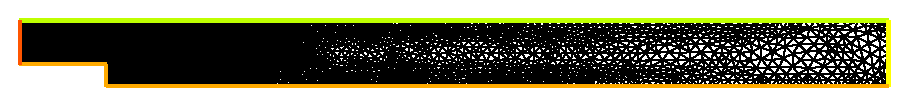
\includegraphics[width=15cm]{NSprojTh}\\
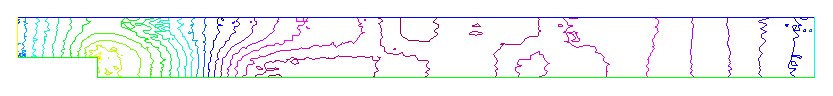
\includegraphics[width=15cm]{NSprojP}\\
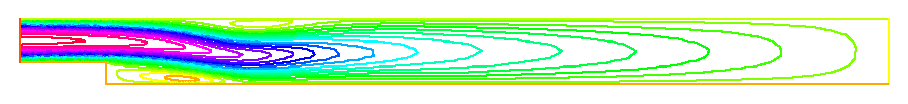
\includegraphics[width=15cm]{NSprojU}

\caption{ Rannacher's projection algorithm: result on an adapted mesh (top) showing
the pressure (middle) and the horizontal velocity $u$ at Reynolds 400.}
\end{center}
\end{figure}

We show in figure \ref{figNSproj} the numerical results obtained for a Reynolds
number of 400 where mesh adaptation is done after 50 iterations on the first mesh.


 \subsection{The System of elasticity}

\paragraph{Elasticity}

Solid objects deform under the action of applied forces:
a point in the solid, originally at $(x,y,z)$ will come to $(X,Y,Z)$
after some time; the vector $U=(u,v,w) = (X-x, Y-y, Z-z)$ is called
the displacement. When the displacement is small and the solid is
elastic, Hooke's law gives a relationship between the stress tensor
$\sigma$ and the strain tensor $\epsilon$
$$
\sigma_{ij} = \lambda \delta_{ij} \nabla.U + \mu\epsilon_{ij},
$$
where $\delta_{ij} = 1$ if $i=j$, $0$ otherwise, with
$$\epsilon_{ij} = {1\over 2}({\p U_i\over\p x_j} +
{\p U_j\over\p x_i} ),
$$
and where $\lambda, \mu$ are two constants that describe the
mechanical properties of the solid, and are themselves related to the
better known constants $E$, Young's modulus, and $\nu$, Poisson's ratio:
$$ \mu = {E\over 1+\nu}, \quad \lambda = {E\nu\over (1+\nu)(1-2\nu)}.
$$

 \paragraph{Lam\'e's system}

Let us consider a beam with axis $Oz$ and with perpendicular section
$\Omega$. The components along $x$ and $y$ of the strain ${\bf u}(x)$
in a section $\Omega$ subject to forces ${\bf f}$ perpendicular to the
axis are governed by \\
$$
  -\lambda \Delta {\bf u} -\mu \nabla (\nabla .{\bf u})={\bf f}~~\hbox{in}~~\Omega,
$$
 where $\lambda ,\mu  $ are the Lam\'{e} coefficients introduced above.
\\

 \paragraph{Example}
 Let us illustrate this by a
 beam with rectangular section that has a fracture at its center and
 subjected to a vertical traction along its horizontal edges. The
 vertical edges are free. We only solve the equations in one quarter
 of the domain thanks to symmetries. We denote respectively by
 $\Gamma_1,\Gamma_2, \Gamma_3,\Gamma_4,\Gamma_5$ the fracture, the
 remainder of the lower edge, the right vertical edge, the upper
 vertical edge and the left vertical edge. The boundary conditions are
\begin{eqnarray}&&
     \lambda{\p {\bf u}\over\p n} + \mu(\nabla\cdot{\bf u}){\bf n} = 0
 ~~\hbox{on}~~\Gamma_1, \cr&&
     v =0,~~\lambda{\p u\over\p n} + \mu\nabla\cdot{\bf u} = 0
 ~~\hbox{on}~~\Gamma_2 \cr&&
     u =0,~~\lambda{\p v\over\p n} + \mu\nabla\cdot{\bf u} = 0
 ~~\hbox{on}~~ \Gamma_3, \Gamma_5 \cr&&
     u =0 \hbox{~~on the left vertical edge}\cr&&
     \lambda{\p {\bf u}\over\p n} + \mu(\nabla\cdot{\bf u}){\bf n} = (0,1)^T
 ~~\hbox{on}~~\Gamma_4
 \end{eqnarray}
Here ${\bf u}=(u,v) $ has two components. Lam\'{e}'s equations are:

 \begin{eqnarray}&&
 -\lambda \Delta u-\mu  {\p ^{2}u\over \p x^{2} }
 - \mu  {\p ^{2}v\over \p x\p y }
 = f_{1},\cr&&
 -\lambda \Delta v-\mu  {\p ^{2}v\over \p y^{2} }
 - \mu  {\p ^{2}u\over \p x\p y }
 = f_{2}.
\end{eqnarray}
%$$\crackb $$
Figure {I.13}{~: \it displacements in a quarter of a beam with a fracture}
\bigskip

The above two equations are strongly coupled by their mixed
derivatives, and thus any iterative solution on each of the
components is risky. One should rather use \freefempp's system
approach and write:

\begin{example}[lame.edp]
\bFF
// file lame.edp
@mesh Th=@square(10,10,[10*x,y]);
@fespace Vh(Th,P2);
Vh u,v,uu,vv;
@macro e11(u) @dx(u)//
@macro e22(v) @dy(v)//
@macro e12(u,v)(@dx(v) + @dy(u))/2 //

@real E = 21.5, sigma = 0.29, mu= E/(2*(1+sigma));
@real lambda = E*sigma/((1+sigma)*(1-2*sigma)), gravity = -9.81;

@solve lame([u,v],[uu,vv])
    = @int2d(Th)( 2*mu*(e11(u)*e11(uu)+e12(u,v)*e12(uu,vv)+e22(v)*e22(vv))
            + lambda*(e11(u)+e22(v))*(e11(uu)+e22(vv))/2)
             - @int2d(Th)(gravity*vv) + @on(4,u=0,v=0);
@plot([u,v],wait=1,ps="lamevect.ps");

@mesh th1 = movemesh(Th, [x+u*1e-4, y+v*1e-4]);
@plot(th1,wait=1,ps="lamedeform.ps");
\eFF
\end{example}

The numerical results are shown on figure \ref{figlame}.

\begin{figure}
\begin{center}\label{figlame}
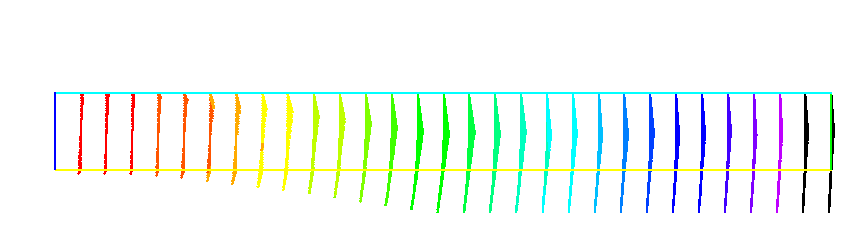
\includegraphics[width=15cm]{lamevect}\\
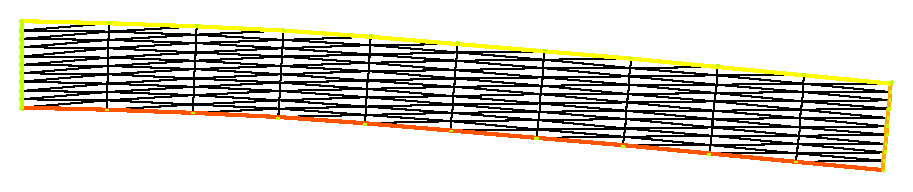
\includegraphics[width=15cm]{lamedeform}

\caption{ Solution of Lam\'e's equation for elasticity for a board deflected by its
own weight and clamped by its left vertical side.}
\end{center}
\end{figure}


\subsection{The System of Stokes for Fluids}

In the case of a flow invariant with respect to the third coordinate
(two-dimensional flow), flows at low Reynolds number (for instance
micro-organisms) satisfy,
\begin{eqnarray*}&&
    \vec -\Delta u + \n p =0
    \cr&&
    \n\cdot \vec u =0
\end{eqnarray*}
where $\vec u=(u_1,u_2)$ is the fluid velocity and $p$ its pressure.
\\
The driven cavity is a standard test. It is a box full of liquid with its lid moving horizontally
at speed one.  The pressure and the velocity must be discretized in compatible fintie
element spaces for the LBB conditions to be satisfied:
\[
    \sup_{p\in P_h}\frac{(\vec u,\n p)}{|p|}\geq \beta|\vec u|~~~\forall \vec u\in U_h
\]
\bFF
//file Stokes.edp
@int n=3;
@mesh Th=@square(10*n,10*n);
@fespace Uh(Th,P1b); Uh u,v,uu,vv;
@fespace Ph(Th,P1);  Ph p,pp;

@solve stokes([u,v,p],[uu,vv,pp]) =
    @int2d(Th)(@dx(u)*@dx(uu)+@dy(u)*@dy(uu) + @dx(v)*@dx(vv)+ @dy(v)*@dy(vv)
            + @dx(p)*uu + @dy(p)*vv + q*(@dx(u)+@dy(v)))
            + @on(1,2,4,u=0,v=0) + @on(3,u=1,v=0);
@plot([u,v],p,wait=1);
\eFF

\begin{figure}[htbp]
\begin{center}\label{figstokes}
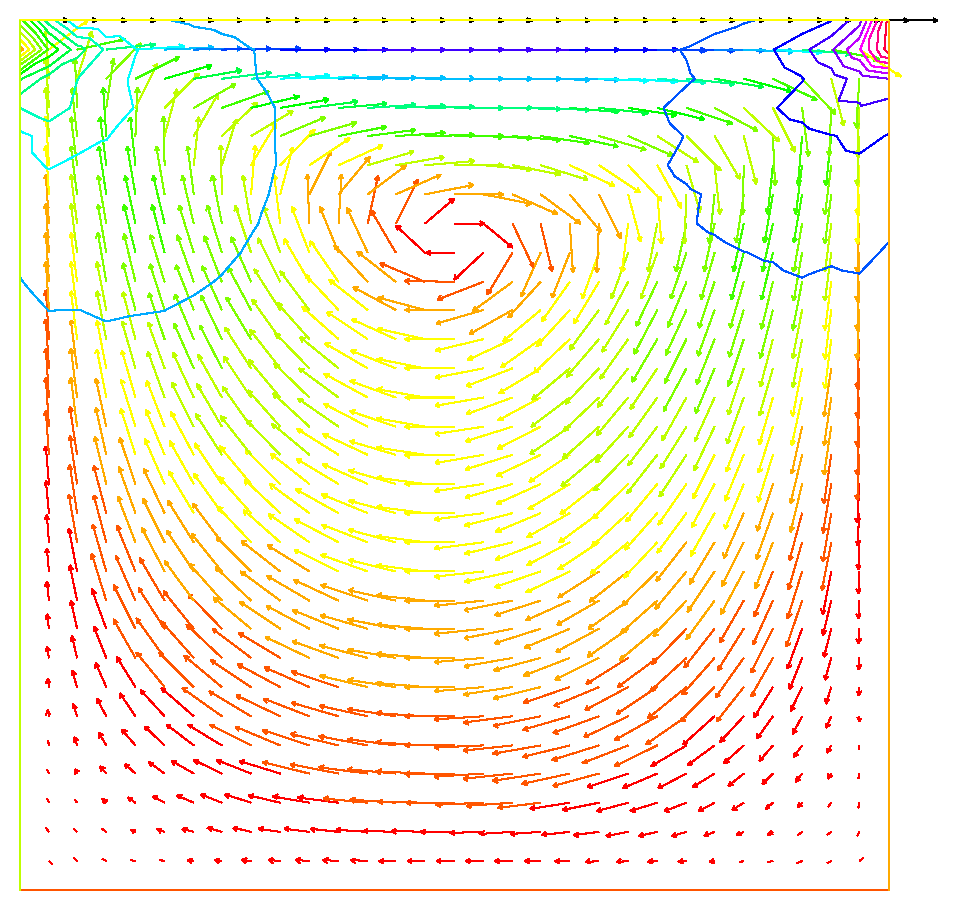
\includegraphics[width=8cm]{stokes}

\caption{ Solution of Stokes' equations for the driven cavity problem, showing the
velocity field and the pressure level lines.}
\end{center}
\end{figure}

Results are shown on figure \ref{figstokes}

\subsection{An Example with Complex Numbers}

 \index{FE function!complex}\index{complex}\index{Helmholtz}
In a microwave oven heat comes from molecular excitation by an
electromagnetic field. For a plane monochromatic wave, amplitude is
given by Helmholtz's equation:
$$ \beta v + \Delta v = 0.
$$
We consider a rectangular oven where the wave is emitted by part of
the upper wall. So the boundary of the domain is made up of a part
$\Gamma_1$ where $v=0$ and of another part $\Gamma_2=[c,d]$ where for
instance $v=\sin(\pi{y-c\over c-d})$.

Within an object to be cooked, denoted by $B$, the heat source is
proportional to $v^2$.
At equilibrium, one has

$$-\Delta\theta = v^2 I_B, \quad \theta_\Gamma = 0
$$
where $I_B$ is $1$ in the object and $0$ elsewhere.
\begin{figure}[htbp]
\begin{center}\label{figmuonde}
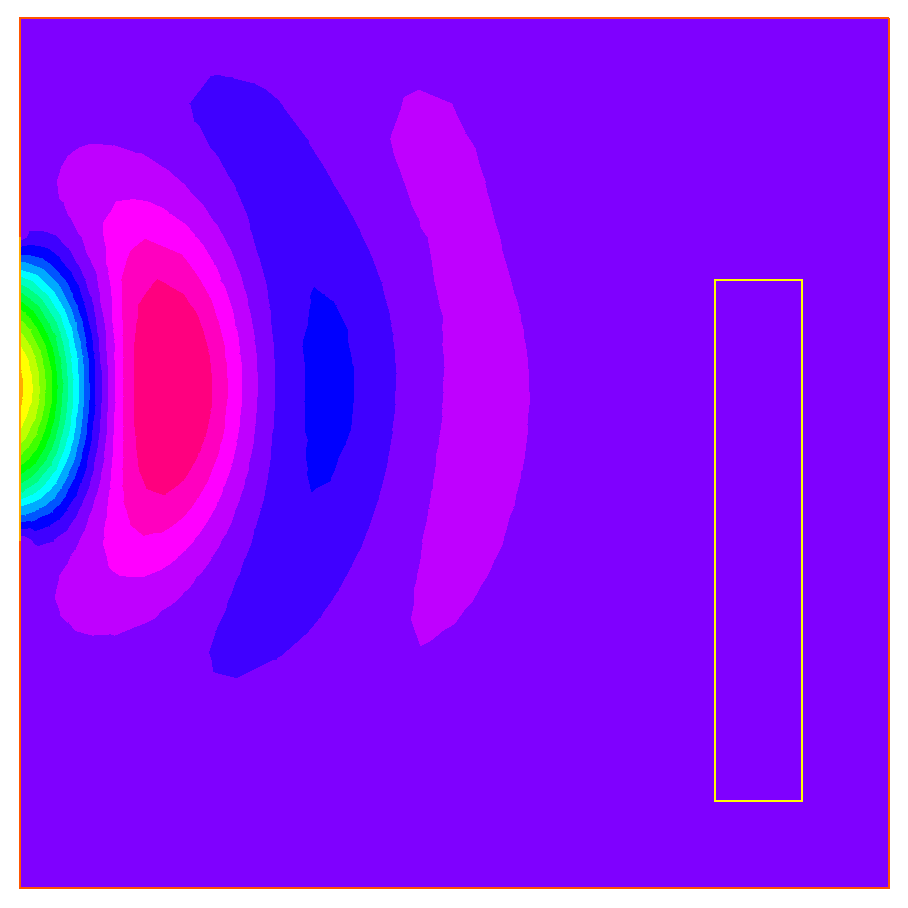
\includegraphics[width=5cm]{rmuonde}
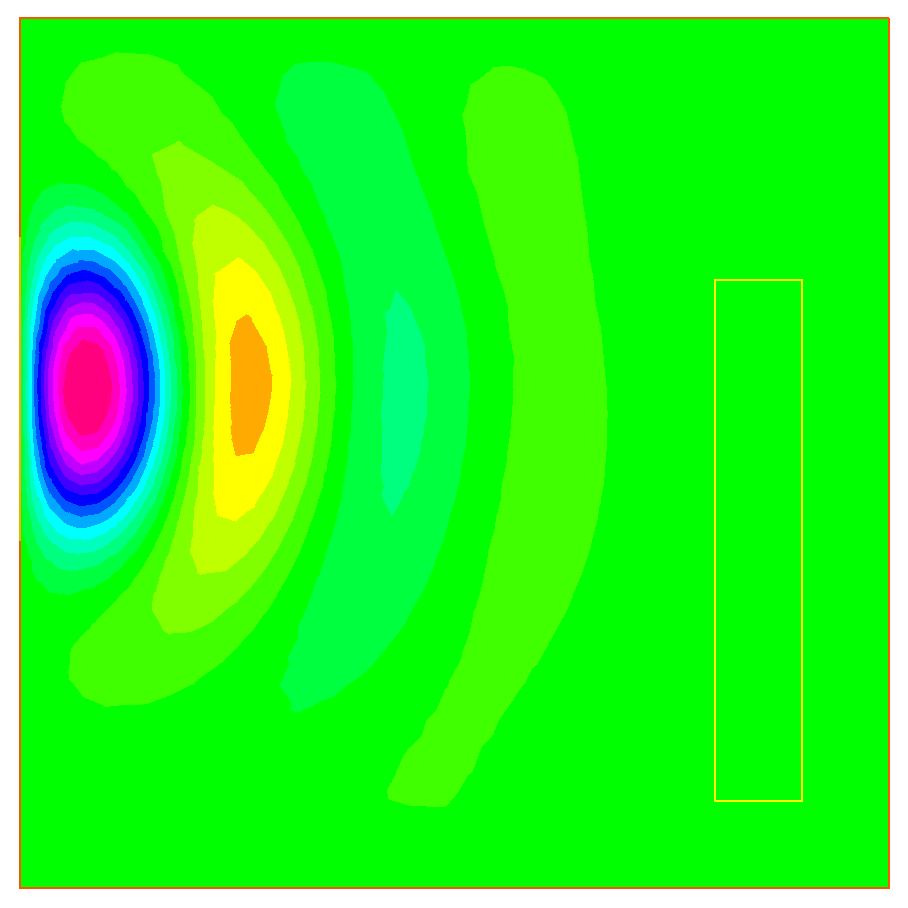
\includegraphics[width=5cm]{imuonde}
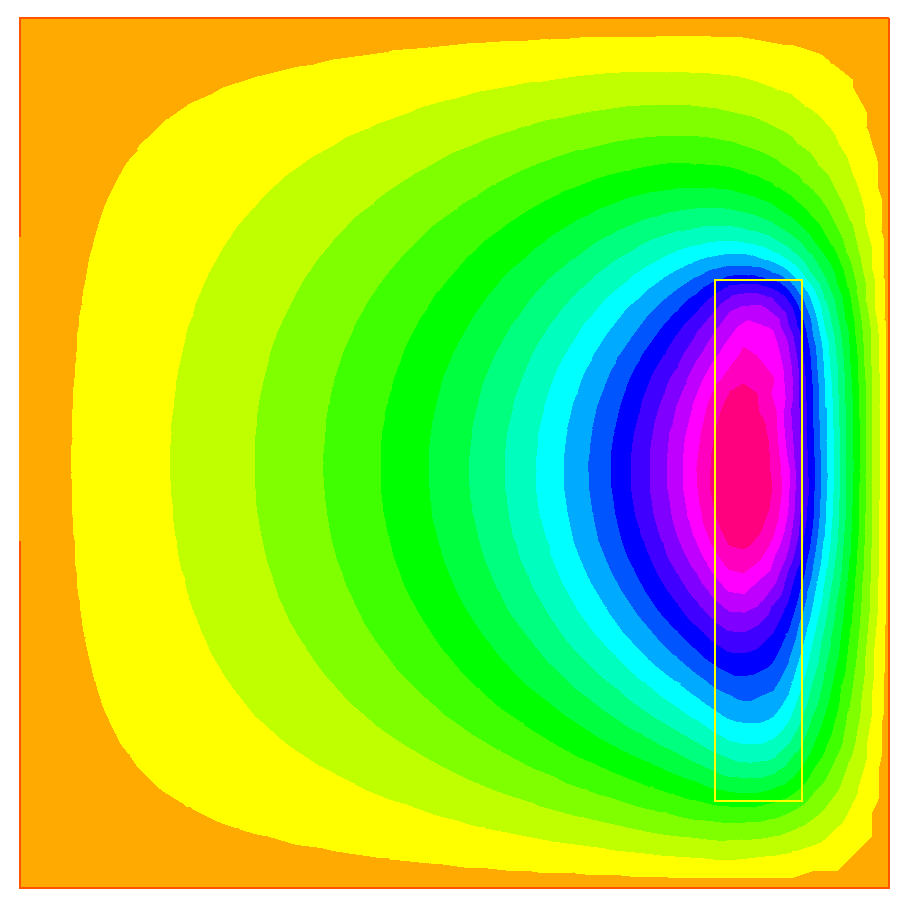
\includegraphics[width=5cm]{tempmuonde}
\caption{A microwave oven: real (left) and imaginary (middle) parts
 of wave  and temperature (right).}
\end{center}
\end{figure}

Results are shown on figure \ref{figmuonde}

In the program below $\beta = 1/(1-I/2)$ in the air and $2/(1-I/2)$
in the object ($i=\sqrt{-1}$):

\begin{example}[muwave.edp]
\bFF

// file muwave.edp
@real a=20, b=20, c=15, d=8, e=2, l=12, f=2, g=2;
@border a0(t=0,1) {x=a*t; y=0;label=1;}
@border a1(t=1,2) {x=a; y= b*(t-1);label=1;}
@border a2(t=2,3) { x=a*(3-t);y=b;label=1;}
@border a3(t=3,4){x=0;y=b-(b-c)*(t-3);label=1;}
@border a4(t=4,5){x=0;y=c-(c-d)*(t-4);label=2;}
@border a5(t=5,6){ x=0; y= d*(6-t);label=1;}

@border b0(t=0,1) {x=a-f+e*(t-1);y=g; label=3;}
@border b1(t=1,4) {x=a-f; y=g+l*(t-1)/3; label=3;}
@border b2(t=4,5) {x=a-f-e*(t-4); y=l+g; label=3;}
@border b3(t=5,8) {x=a-e-f; y= l+g-l*(t-5)/3; label=3;}
@int n=2;
@mesh Th = @buildmesh(a0(10*n)+a1(10*n)+a2(10*n)+a3(10*n)
        +a4(10*n)+a5(10*n)+b0(5*n)+b1(10*n)+b2(5*n)+b3(10*n));
@plot(Th,wait=1);
@fespace Vh(Th,P1);
@real meat =  Th(a-f-e/2,g+l/2).@region, air= Th(0.01,0.01).@region;
Vh R=(region-air)/(meat-air);

Vh<@complex> v,w;
@solve muwave(v,w) = @int2d(Th)(v*w*(1+R)
                -(@dx(v)*@dx(w)+@dy(v)*@dy(w))*(1-0.5i))
   + @on(1,v=0) + @on(2, v=sin(pi*(y-c)/(c-d)));
Vh vr=@real(v), vi=@imag(v);
@plot(vr,wait=1,ps="rmuonde.ps", fill=true);
@plot(vi,wait=1,ps="imuonde.ps", fill=true);

@fespace Uh(Th,P1); Uh u,uu, ff=1e5*(vr^2 + vi^2)*R;

@solve temperature(u,uu)= @int2d(Th)(@dx(u)* @dx(uu)+ @dy(u)* @dy(uu))
     - @int2d(Th)(ff*uu) + @on(1,2,u=0);
@plot(u,wait=1,ps="tempmuonde.ps", fill=true);
\eFF
\end{example}

\subsection{Optimal Control} Thanks to the function \texttt{BFGS} it
is possible to solve complex nonlinear optimization problem within
\texttt{freefem++}. For example consider the following inverse
problem
\[
    \min_{b,c,d\in R}J=\int_E(u-u_d)^2~:~
    -\nabla(\kappa(b,c,d)\cdot\nabla u)=0,~~u|_\Gamma=u_\Gamma
\]
where the desired state $u_d$, the boundary data $u_\Gamma$ and the
observation set $E\subset\Omega$ are all given.  Furthermore let us
assume that
\[
    \kappa(x)=1+bI_B(x)+cI_C(x)+dI_D(x)~~~\forall x\in\Omega
\]
where $B,C,D$ are separated subsets of $\Omega$.
\\\\
To solve this problem by the quasi-Newton BFGS method we need the
derivatives of $J$ with respect to $b,c,d$.  We self explanatory
notations, if $\delta b,\delta c,\delta d$ are variations of
$b,c,d$ we have
\[
    \delta J\approx 2\int_E(u-u_d)\delta u,~~
    -\nabla(\kappa\cdot\nabla\delta u)\approx\nabla(\delta\kappa\cdot\nabla
    u)
    ~~\delta u|_\Gamma=0
\]
Obviously $J'_b$ is equal to $\delta J$ when $\delta b=1,\delta
c=0,\delta d=0$, and so on for $J'_c$ and $J'_d$.
\\\\
All this is implemented in the following program
 \bFF
// file optimcontrol.edp
@border aa(t=0, 2*pi) {    x = 5*cos(t);    y = 5*sin(t);  };
@border bb(t=0, 2*pi) {    x = cos(t);    y = sin(t);  };
@border cc(t=0, 2*pi) {    x = -3+cos(t);    y = sin(t);  };
@border dd(t=0, 2*pi) {    x = cos(t);    y = -3+sin(t);  };
@mesh th = @buildmesh(aa(70)+bb(35)+cc(35)+dd(35));
@fespace Vh(th,P1);
Vh Ib=((x^2+y^2)<1.0001),
   Ic=(((x+3)^2+ y^2)<1.0001),
   Id=((x^2+(y+3)^2)<1.0001),
   Ie=(((x-1)^2+ y^2)<=4),
   ud,u,uh,du;
@real[int] z(3);
@problem A(u,uh) =@int2d(th)((1+z[0]*Ib+z[1]*Ic+z[2]*Id)*(dx(u)*dx(uh)
                    +dy(u)*dy(uh))) + on(aa,u=x^3-y^3);
z[0]=2; z[1]=3; z[2]=4;
A; ud=u;
@ofstream f("J.txt");
@func @real J(real[int] & Z)
{
    @for (int i=0;i<z.n;i++)z[i]=Z[i];
    A; @real s= @int2d(th)(Ie*(u-ud)^2);
    f<<s<<"   "; @return s;
}

@real[int] dz(3), dJdz(3);

@problem B(du,uh)
  =@int2d(th)((1+z[0]*Ib+z[1]*Ic+z[2]*Id)*(dx(du)*dx(uh)+dy(du)*dy(uh)))
  +@int2d(th)((dz[0]*Ib+dz[1]*Ic+dz[2]*Id)*(dx(u)*dx(uh)+dy(u)*dy(uh)))
  +@on(aa,du=0);

@func @real[int] DJ(@real[@int] &Z)
    {
      @for(int i=0;i<z.n;i++)
        { @for(int j=0;j<dz.n;j++) dz[j]=0;
          dz[i]=1; B;
          dJdz[i]= 2*int2d(th)(Ie*(u-ud)*du);
      }
     @return dJdz;
 }

 @real[@int] Z(3);
 @for(@int j=0;j<z.n;j++) Z[j]=1;
 BFGS(J,DJ,Z,eps=1.e-6,nbiter=15,nbiterline=20);
 @cout << "BFGS: J(z) = " << J(Z) <<  endl;
 @for(int j=0;j<z.n;j++) cout<<z[j]<<endl;
 @plot(ud,value=1,ps="u.eps");
\eFF
In this example the sets $B,C,D,E$ are circles of boundaries $bb,cc,dd,ee$ are the domain
$\Omega$ is the circle of boundary $aa$.  The desired state $u_d$ is the solution
of the PDE for $b=2,c=3,d=4$.  The unknowns are packed into array $z$.  Notice that it is
necessary to recopy $Z$ into $z$ because one is a local variable while the other one is global.
The program found $b=2.00125,c=3.00109,d=4.00551$.
Figure \ref{figcontrol} shows $u$ at convergence
and the successive function evaluations of $J$.
\begin{figure}\label{figcontrol}
\begin{center}
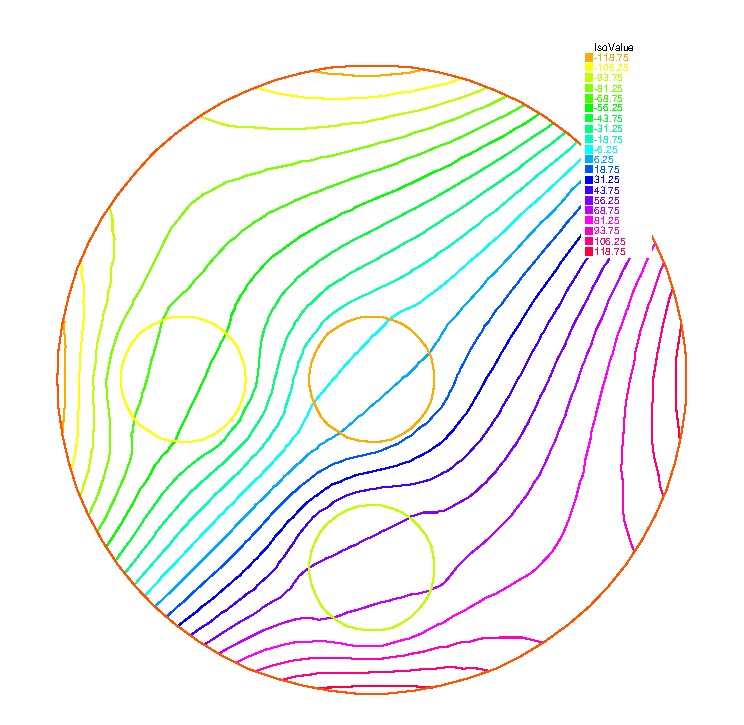
\includegraphics[width=5cm]{u-bfgs}
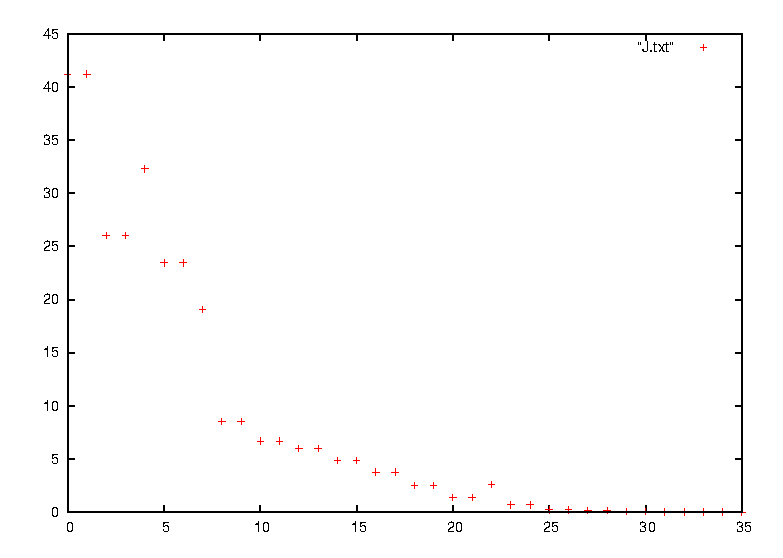
\includegraphics[width=5cm]{J-bfgs}
\caption{On the left the level lines of $u$. On the right the successive evaluations of
$J$ by BFGS (5 values above 500 have been removed for readability)}
\end{center}
\end{figure}
Note that an \emph{adjoint state} could have been used. Define $p$ by
\[
-\nabla\cdot(\kappa\nabla p)=2I_E(u-u_d),~~~p|_Gamma=0
\]
Consequently
\begin{eqnarray}&&
\delta J = -\int_\Omega (\nabla\cdot(\kappa\nabla p))\delta u
\cr&&
= \int_Omega(\kappa\nabla p\cdot\nabla\delta u)
=-\int_Omega(\delta\kappa\nabla p\cdot\nabla u)
\end{eqnarray}
Then the derivatives are found by setting $\delta b=1, \delta c=\delta d=0$ and so on:
\[
    J'_b=-\int_B \nabla p\cdot\nabla u,~~J'_c=-\int_C \nabla p\cdot\nabla u,~~
    J'_d=-\int_D \nabla p\cdot\nabla u
\]
\paragraph{Remark} As BFGS stores an $M\times M$ matrix where $M$ is the number of
unknowns, it is dangerously expensive to use this method when the unknown $x$ is a
Finite Element Function.  One should use another optimizer such as
the NonLinear Conjugate Gradient \texttt{NLCG} (also a key word
of freefem++).  See the file algo.edp in the examples folder.

 \subsection{Classification of the equations}
\paragraph{Summary}\emph{
It is usually not easy to determine the type of a system.  Yet the approximations
and algorithms suited to the problem depend on its type:
\begin{itemize}
\item Finite Elements compatible (LBB conditions) for elliptic systems
\item Finite difference on the parabolic variable and a time loop on each
elliptic subsystem of parabolic systems; better stability diagrams when the schemes are implicit in time.
\item Upwinding, Petrov-Galerkin, Characteristics-Galerkin, Discontinuous-Galerkin, Finite Volumes
for hyperbolic systems plus, possibly, a time loop.
\end{itemize}
When the system changes type, then expect difficulties (like shock discontinuities)!}

 \paragraph{Elliptic, parabolic and hyperbolic equations}

A partial differential equation (PDE) is a relation between a function
of several variables and its derivatives.
 $$
 F(\varphi(x),{\p\varphi\over\p
 x_1}(x),\cdots,{\p\varphi\over\p
 x_d}(x),{\p^2\varphi\over\p
 x^2_1}(x),\cdots,{\p^m\varphi\over\p x^m_d}(x)) =
 0\quad\forall x\in\Omega\subset \Rel^d.
 $$
 The range of $x$ over which the equation is taken, here $\Omega$, is called
 the \emph{domain} of the PDE.
The highest derivation index, here $m$, is called the {\it
 order}. If $F$ and $\varphi$ are vector valued functions, then the
 PDE is actually a \emph{system} of PDEs.
 \\
Unless indicated otherwise, here by convention \emph{one} PDE
 corresponds to one scalar valued $F$ and $\varphi$.
If $F$ is linear with respect to its arguments, then the PDE is said
 to be \emph{linear}.
 \\
The general form of a second order, linear scalar PDE is
${\p^2\varphi\over\p x_i\p x_j}$ and $A:B$ means
 $\sum^d_{i,j=1} a_{ij} b_{ij}.$
 $$\alpha\varphi + a\cdot\nabla\varphi + B :\nabla(\nabla\varphi) =
 f{\quad\hbox{ in }\quad}\Omega\subset \Rel^d,
 $$
 where $f(x),\alpha(x)\in \Rel,
 a(x)\in \Rel^d, B(x)\in \Rel^{d\times d}$
are the PDE \emph{coefficients}.
If the coefficients are independent of $x$, the PDE is said to have
 \emph{constant coefficients}.

To a PDE we associate a quadratic form, by replacing
$\varphi$ by $1$,
 $\p\varphi/\p x_i$ by $z_i$ and
 $\p^2\varphi/\p x_i\p x_j$ by $z_i z_j$, where $z$
 is a vector in $\Rel^d$~:
 $$\alpha + a\cdot z + z^T Bz = f.
 $$
If it is the equation of an ellipse (ellipsoid if $d \geq 2$),
the PDE is said to be {\it elliptic};
if it is the equation of a parabola or a hyperbola, the PDE is said to
be {\it parabolic} or {\it hyperbolic}. If $A \equiv 0$, the degree is
no longer 2 but 1, and for reasons that will appear more clearly
later, the PDE is still said to be hyperbolic.
\\\\
These concepts can be generalized to systems, by studying whether or
not the polynomial system $P(z)$ associated with the PDE system has
branches at infinity (ellipsoids have no branches at infinity,
paraboloids have one, and hyperboloids have several).
\\
If the PDE is not linear, it is said to be \emph{non linear}.
Those are said to be locally elliptic, parabolic, or hyperbolic
according to the type of the linearized equation.
\\
For example, for the non linear equation
 $${\p^2\varphi\over\p t^2} - {\p\varphi\over\p
 x}{\p^2\varphi\over\p x^2} = 1,
 $$
  we have $d=2, x_1 = t, x_2 = x$ and its linearized form is:
 $${\p^2 u\over\p t^2} - {\p u\over\p x}
 {\p^2\varphi\over\p x^2} - {\p\varphi\over\p
 x}{\p^2 u\over\p x^2} = 0,
 $$
which for the unknown $u$ is locally elliptic if
 ${\p\varphi\over\p x} < 0$  and locally hyperbolic if
 ${\p\varphi\over\p x} > 0$.

\paragraph{Examples}

 \noindent{Laplace's} equation is elliptic:
 $$\Delta\varphi \equiv {\p^2\varphi\over\p x^2_1} +
 {\p^2\varphi\over\p x^2_2} + \cdots +
 {\p^2\varphi\over\p x^2_d} = f, \ \ \ \forall x
 \in \Omega\subset \Rel^d.
 $$
The \emph{heat} equation is parabolic in
 $Q = \Omega\times]0,T[\subset \Rel^{d+1}$~:
 $${\p\varphi\over\p t} - \mu\Delta\varphi = f\quad\forall
 x\in\Omega\subset  \Rel^d, \quad\forall t\in]0,T[.
 $$
If $\mu >0$,  the \emph{wave} equation is hyperbolic:
 $${\p^2\varphi\over\p t^2} - \mu\Delta\varphi =
 f{\quad\hbox{~in~}\quad}  Q.
 $$
The \emph{convection diffusion} equation is parabolic if $\mu \neq 0$
 and hyperbolic otherwise:
 $${\p\varphi\over\p t} + a\nabla\varphi -
 \mu\Delta\varphi = f.
 $$
The \emph{biharmonic} equation is elliptic:
 $$\Delta(\Delta\varphi) = f{\quad\hbox{~in~}\quad}\Omega.
 $$

\paragraph{Boundary conditions}

A relation between a function and its derivatives is not sufficient to define the function.
Additional information on the boundary $\Gamma=\p\Omega$ of
$\Omega$, or on part of $\Gamma$ is necessary.\\
Such information is called a \emph{boundary condition}.
For example,
 $$\varphi(x) \ \hbox{given},\ \forall x\in \Gamma,
 $$
is called a \emph{\x{Dirichlet} boundary condition}.
The \emph{\x{Neumann}} condition is
 $${\p\varphi\over\p n}(x) \ \hbox{given on }\
 \Gamma \hbox{~~~(or~~} n\cdot B\nabla\varphi,\hbox{given on }\
 \Gamma\hbox{ for a general second order PDE)}
$$
  where $n$ is the normal at $x\in\Gamma$
directed towards the exterior of $\Omega$ (by definition
 ${\p\varphi\over\p n}=\nabla\varphi\cdot n$).

Another classical condition, called a \emph{Robin} (or \emph{Fourier})
condition is written as:
 $$\varphi(x) + \beta(x) {\p\varphi\over\p n}(x) \
 \hbox{given on}\
 \Gamma.
 $$
Finding a set of boundary conditions  that defines a unique
 $\varphi$ is a difficult art.\\
In general, an elliptic equation is well posed (\emph{i.e.} $\varphi$
 is unique) with one Dirichlet, Neumann or Robin conditions on the whole boundary.
 \\
Thus, Laplace's equations  is well posed with
 a Dirichlet or Neumann condition but also with
 $$\varphi \ \hbox{given on}\ \Gamma_1,\quad {\p\varphi\over
 \p n} \
 \hbox{given on}\ \Gamma_2, \quad \Gamma_1\cup\Gamma_2 =
 \Gamma,\quad{\dot{\Gamma_1}\cap\dot{\Gamma_2}} =
 \emptyset.$$
Parabolic and hyperbolic equations rarely require boundary conditions
 on all of  $\Gamma\times]0,T[$. For instance, the heat equation
 is well posed with
 $$\varphi \ \hbox{given at}\ t=0 \ \hbox{and Dirichlet or Neumann or mixed conditions on}\
 \p\Omega.$$
Here $t$ is time so the first condition is called an \x{initial condition}.  The whole set of conditions
are also called \x{Cauchy} conditions.
\\
The wave equation  is well posed with
 $$\varphi \ \hbox{and}\ {\p\varphi\over\p t} \
 \hbox{given at}\ t=0
 \ \hbox{and Dirichlet or Neumann or mixed conditions on}\
 \p\Omega.
 $$


\textBlack
\section{Syntax}
\subsection{Data Types}
In essence \freefempp  is a \index{compiler} compiler:
  its language is typed, polymorphic and reentrant.
Every variable must be declared of a certain type,  in a  declarative statement;
each statement are separated
from the next by a semicolon `\texttt{;}'.
The language allows the manipulation of basic types
integers (\texttt{int}), reals (\texttt{real}), strings (\texttt{string}),
arrays (example: \texttt{real[int]}),
 bidimensional (2D) finite element meshes (\texttt{mesh}),
2D finite element spaces (\texttt{fespace}) , analytical functions
(\texttt{func}), arrays of
finite element functions (\texttt{func$[basic\_type]$}),
linear and bilinear operators, sparse matrices, vectors , etc. For instance

\bFF
  @int i,n=20;               //  $ i,n$ are integer.
  @real[@int] xx(n),yy(n);    //  two array of size n
  @for (i=0;i<=20;i++)       // which can be used in statements such as
   { xx[i]= cos(i*pi/10); yy[i]= sin(i*pi/10); }
\eFF
The life of a variable is the current block $\{\ldots \}$, except the \texttt{fespace}
variable, and the variables local to a block are destroyed at the end of the block as follows.
\begin{example}~~
\bFF
@real r= 0.01;
@mesh Th=@square(10,10); // unit square mesh
@fespace Vh(Th,@P1);     // P1 lagrange finite  element space
Vh u = x+ exp(y);
@func f = z * x + r * log(y);
@plot(u,wait=true);
{  // new block
  @real r = 2; // not the same r
  @fespace Vh(Th,@P1);//  error because Vh is a global name
}  // end of block
//  here r back to 0.01
\eFF
\end{example}
The type declarations are  compulsory in \freefempp  because it is easy
to make bugs in a language with many types. \index{variable} The
variable name is just an alphanumeric \index{alphanumeric} string, the
underscore character  ``\texttt{\_}'' is not allowed, because
it will be used as an operator in the future.\index{\_}

\subsection{List of major types}
\begin{description}
\item[bool]   is used for logical expression and flow-control.  The result of a
comparison is a boolean type as in
\bFF
bool fool=(1<2);
\eFF
which makes fool to be true.  Similar examples can be built with $==,<=,>=,<,>,!=$.
\index{bool}\index{true}\index{false}
\item[int]
  declares an integer.
\item[string] declare the variable to store
a text enclosed within double quotes, such as:
\bFF
"This is a string in double quotes."
\eFF
\index{string}
\item[real] declares the variable to store a number such as ``12.345''. \index{real}
\item[complex]  Complex numbers, such as\index{Complex}
$1+2i$, \freefempp understand that $i=\sqrt{-1}$.
\bFF
@complex a =  1@i, b = 2 + 3@i;
@cout << "a + b = " << a + b << @endl;
@cout << "a - b = " << a + b << @endl;
@cout << "a * b = " << a * b << @endl;
@cout << "a / b = " << a / b << @endl;
\eFF
Here's the output;
\bFF
a + b = (2,4)
a - b = (-2,-2)
a * b = (-3,2)
a / b = (0.230769,0.153846)
\eFF
\item[ofstream]  to declare an output file .
\item[ifstream]   to declare an input file .

\item[real[int]]  declares a variable that stores multiple
real numbers with integer index.
\index{array}
\bFF
@real[@int] a(5);
a[0] = 1; a[1] = 2; a[2] = 3.3333333; a[3] = 4; a[4] = 5;
@cout << "a = " << a  << @endl;
\eFF
This produces the output;
\bFF
a = 5   :
  1       2     3.33333   4       5
\eFF
\item[real[string]]  declares a variable that store multiple
real numbers with string index.
\item[string[string]]  declares a variable that store multiple
strings with string index.
\index{array}
\itemtt[func] defines a function without argument,
if independent variables are \ttCC{x, y}.
For example
\bFF
@func f=cos(x)+sin(y) ;
\eFF
\index{func}
Remark that the function's type is given by the expression's type.
Raising functions to a numerical power is done, for instance, by
\ttCC{x\^{}1}, \ttCC{y\^{}0.23}.

\itemtt[mesh]  \index{mesh}
creates the triangulation, see \refSec{Mesh Generation}.
\itemtt[fespace]
defines a new type of finite element space, see Section \refSec{Finite Elements}.
\itemtt[problem]  declares the weak form of a partial differential problem without solving it.
\index{problem}
\itemtt[solve]  declares a problem and solves it.\index{solve}
\itemtt[varf]   defines a full variational form. \index{varf}
\itemtt[matrix] defines a sparse matrix. \index{matrix}
\end{description}

\subsection{Global Variables}\label{sec:Global}
 The names \ttCC{x,y,z,label,region,P,N,nu\_triangle} are reserved words used to link
the language to the finite element tools:
\begin{description}
    \itemtt[x]  is the $x$ coordinate of the current point (real value) \index{x}
    \itemtt[y]  is the $y$ coordinate  of the current point (real value) \index{y}
    \itemtt[z]  is the $z$ coordinate of the current point (real value) \index{z}, but is reserved for future use.
\itemtt[label] contains the label number of a boundary if the  current point is
on a boundary, 0 otherwise  (int value). \index{label}
    \item[region]   returns the region number of  the current point (x,y) (int value). \index{region}
\itemtt[P]  gives the  current point  ($\R^{2}$ value. \index{P}).
By \texttt{P.x}, \texttt{P.y}, we can get the $x,\, y$ components of \texttt{P} .
Also \texttt{P.z} is reserved.
    \itemtt[N]  gives the outward unit normal vector at the  current point if it is on a
     curve define by \texttt{border} ($\R^{3}$ value).
\texttt{N.x} and \texttt{N.y} are $x$ and $y$ components of the normal vector.
\texttt{N.z} is reserved. \index{N}.
    \itemtt[lenEdge] gives the length of the current edge\index{lenEdge}\\
    \[
    \texttt{lenEdge} = |q^i-q^j|\quad \textrm{if the current edge is }[q^i,q^j]
    \]

    \itemtt[hTriangle] gives the size of the current triangle \index{hTriangle}

    \itemtt[nuTriangle] gives the index of the current triangle (integer).
    \index{nuTriangle}

    \itemtt[nuEdge]  gives the index of the current edge in the triangle (integer).
    \index{nuEdge}

    \itemtt[nTonEdge] gives the number of adjacent triangle of the current
    edge (integer ).\index{nTonEdge}

    \itemtt[area] give the area of the current triangle (real). \index{area}

\itemtt[cout]  is the standard output device (default is console).
On MS-Windows, the standard output is only to console, in this time.
  \Ostream
\itemtt[cin]  is the standard input device (default is keyboard). (\Istream).
On MS-Windows, this doesn't work).
\itemtt[endl] give the end of line in the input/output devices.
\itemtt[true]   means ``true'' in  \Bool\  value.
\itemtt[false]  means ``false'' in  \Bool\ value.
\itemtt[pi]   is the \Real ~approximation value of $\pi$.
\end{description}

\subsection{System Commands}

Here is how to show all the types, and all the operator and functions of a \freefempp program:
\bFF
 @dumptable(@cout);
\eFF \index{dumptable}
To execute a system command in the string (not implemented on Carbon MacOS)
\bFF
  @exec("shell command");
\eFF
On MS-Windows, we need the full path. For example, if there is the command
``ls.exe'' in the subdirectory ``\verb|c:\cygwin\bin\|'', then we must write
\bFF
  @exec("c:\\cygwin\\bin\\ls.exe");
\eFF
\index{exec}

Another useful system command is \x{assert()} to make sure something is true.

\bFF
@assert(version>=1.40);
\eFF


\subsection{Arithmetic}
On integers, $+,\, -,\, *$ express the usual arithmetic summation (plus),
subtraction (minus) and multiplication (times), respectively,The operators $/$ and $\%$ yield the quotient and the remainder from the division of the first expression by the second.
If the second number of $/$ or $\%$ is zero the behavior is undefined.
The \key{maximum} or \key{minimum} of two integers $a,\, b$ are obtained
by \texttt{max($a$,$b$)} of
\texttt{min($a$,$b$)}.
The power $a^b$ of two integers $a,\, b$ is calculated by writing \verb|a^b|.
The classical \texttt{C++}
"arithmetical if"  expression \ttCC{ a ? b : c} is equal to  the value of expression \ttCC{b} if
the value of expression  \ttCC{a} is true otherwise is equal to value of expression \ttCC{c}.
\index{?:}

\begin{example} Calculations with the integers
\label{exm:int}
\bFF
@int a = 12, b = 5;
@cout <<"plus, minus of "<<a<<" and "<<b<<" are "<<a+b<<", "<<a-b<<@endl;
@cout <<"multiplication, quotient of them are "<<a*b<<", "<<a/b<<@endl;
@cout <<"remainder from division of "<<a<<" by "<<b<<" is "<<a%b<<@endl;
@cout <<"the minus of "<<a<<" is "<< -a << @endl;
@cout <<a<<" plus -"<<b<<" need bracket:"<<a<<"+(-"<<b<<")="<<a+(-b)<<@endl;
@cout <<"max and min of "<<a<<" and "<<b<<" is "<<@max(a,b)<<","<<@min(a,b)<< @endl;
@cout <<b<<"th power of "<<a<<" is "<<a^b<< @endl;
@cout << " min  == (a < b ? a : b )  is " << (a < b ? a : b) << @endl;

b=0;
@cout <<a<<"/0"<<" is "<< a/b << @endl;
@cout <<a<<"\%0"<<" is "<< a\%b << @endl;
\eFF
produce the following result:
\bFF
plus, minus of 12 and 5 are 17, 7
multiplication, quotient of them are 60, 2
remainder from division of 12 by 5 is 2
the minus of 12 is -12
12 plus -5 need bracket :12+(-5)=7
max and min of 12 and 5 is 12,5
5th power of 12 is 248832
min == (a < b ? a : b)   is 5
12/0 : long long long
Fatal error : ExecError  Div by 0 at exec line  9
Exec error : exit
\eFF
\end{example}

By the relation $integer\subset real$, the operators
``$+,\, -,\, *,\, /,\, \%$'' and ``\ttCC{@max,\, @min,\, \^}''
are also applicable on real-typed variables. However,  $\%$
calculates the remainder of the integer parts of two real numbers.

The following are examples similar to Example \ref{exm:int}
\bFF
@real a=sqrt(2.), b = pi;
@cout <<"plus, minus of "<<a<<" and "<<pi<<" are "<< a+b <<", "<< a-b << @endl;
@cout <<"multiplication, quotient of them are "<<a*b<<", "<<a/b<< @endl;
@cout <<"remainder from division of "<<a<<" by "<<b<<" is "<< a%b << @endl;
@cout <<"the minus of "<<a<<" is "<< -a << @endl;
@cout <<a<<" plus -"<<b<<" need bracket :"<<a<<"+(-"<<b<<")="<<a + (-b) << @endl;
\eFF
It gives the following output:
\bFF
plus, minus of 1.41421 and 3.14159 are 4.55581, -1.72738
multiplication, quotient of them are 4.44288, 0.450158
remainder from division of 1.41421 by 3.14159 is 1
the minus of 1.41421 is -1.41421
1.41421 plus -3.14159 need bracket :1.41421+(-3.14159)=-1.72738
\eFF

By the relation
$$
bool\subset int \subset real\subset complex,
$$
the operators
``$+,\, -,\, *,\, /$'' and ``\ttCC{\^}'' are also applicable on complex-typed variables,
but ``\%,\, max, min'' fall into misuse.
Complex numbers such as \texttt{5+9i},\, i$=\sqrt{-1}$, can be a little tricky.
For real variables \texttt{a=2.45, b=5.33}, we must write the complex numbers
$a+i~b$ and $a+i\sqrt{2.0}$ as
\bFF
@complex z1 = a+b*1i, z2=a+@sqrt(2.0)*1i;
\eFF
The imaginary and real parts of complex number \texttt{z} is obtained by
\ttCC{@imag} and \ttCC{@real}. \index{imag}\index{real}\index{complex}
The conjugate of $a+bi$ ($a,b$ are real) is defined by $a-bi$, which
is denoted by \ttCC{@conj(a+b*1i)} in \freefempp.

The complex number $z=a+ib$ is considered as
the pair $(a,b)$ of real numbers $a,\, b$.
We can attach to it the point $(a,b)$ in the Cartesian plane where the $x$-axis is for the
 real part and the
$y$-axis for the imaginary part.
The same point $(a,b)$ has a representation with polar coordinate $(r,\phi)$,
So $z$ his also $z=r(\cos \phi+i\sin\phi )$,
$r=\sqrt{a^2+b^2}$ and $\phi=\tan^{-1}(b/a)$;
$r$ is called the \key{modulus} and $\phi$ the \key{argument} of $z$.
In the following example, we shall show them using \freefempp programming,
and \key{de Moivre's formula} $z^n=r^n(\cos n\phi+i\sin n\phi)$.

\begin{example}~
\label{exm:complex}
\bFF
@real a=2.45, b=5.33;
@complex  z1=a+b*1i, z2 = a+sqrt(2.)*1i;
@func @string pc(@complex z) // printout complex to (real)+i(imaginary)
{
   @string r = "("+real(z);
   if (@imag(z)>=0) r = r+"+";
   @return r+@imag(z)+"i)";
}
// printout complex to |z|*(cos(arg(z))+i*sin(arg(z)))
@func @string toPolar(@complex z)
{
   @return @abs(z)+"*(cos("+@arg(z)+")+i*sin("+@arg(z)+"))";
}
cout <<"Standard output of the complex "<<pc(z1)<<" is the pair "
     <<z1<<endl;
cout <<"Plus, minus of "<<pc(z1)<<" and "<<pc(z2)<<" are "<< pc(z1+z2)
     <<", "<< pc(z1-z2) << endl;
cout <<"Multiplication, quotient of them are "<<pc(z1*z2)<<", "
     <<pc(z1/z2)<< endl;
cout <<"Real/imaginary part of "<<pc(z1)<<" is "<<@real(z1)<<", "
     <<@imag(z1)<<endl;
cout <<"Absolute of "<<pc(z1)<<" is "<<@abs(z1)<<endl;
cout <<pc(z2)<<" = "<<toPolar(z2)<<endl;
cout <<"  and polar("<<@abs(z2)<<","<<@arg(z2)<<") = "
     << pc(@polar(abs(z2),arg(z2)))<<endl;
cout <<"de Moivre's formula: "<<pc(z2)<<"^3 = "<<toPolar(z2^3)<<endl;
cout <<"conjugate of "<<pc(z2)<<" is "<<pc(@conj(z2))<<endl;
cout <<pc(z1)<<"^"<<pc(z2)<<" is "<< pc(z1^z2) << endl;
\eFF
Here's the output from Example \ref{exm:complex}
\bFF
Standard output of the complex (2.45+5.33i) is the pair (2.45,5.33)
Plus, minus of (2.45+5.33i) and (2.45+1.41421i) are (4.9+6.74421i), (0+3.91579i)
Multiplication, quotient of them are (-1.53526+16.5233i), (1.692+1.19883i)
Real/imaginary part of (2.45+5.33i) is 2.45, 5.33
Absolute of (2.45+5.33i) is 5.86612
(2.45+1.41421i) = 2.82887*(cos(0.523509)+i*sin(0.523509))
  and polar(2.82887,0.523509) = (2.45+1.41421i)
de Moivre's formula: (2.45+1.41421i)^3
                         = 22.638*(cos(1.57053)+i*sin(1.57053))
conjugate of (2.45+1.41421i) is (2.45-1.41421i)
(2.45+5.33i)^(2.45+1.41421i) is (8.37072-12.7078i)
\eFF
\end{example}

\subsection{\setS{One Variable Functions}}
\index{functions}
\begin{description}
  \item[Fundamental functions] are built into \freefempp.
The \emph{power function} \ttCC{x\^}$\alpha (=x^\alpha)$;
the \emph{exponent function} \ttCC{@exp(x)} ($=e^x$);
the \emph{logarithmic function} \ttCC{@log(x)}($=\ln x$) or
\ttCC{@log10(x)} ($=\log_{10}x$);
the \emph{trigonometric functions} \ttCC{@sin(x), @cos(x), @tan(x)}
depending on angles measured by \emph{radian};
the inverse of $\sin x,\, \cos x,\, \tan x$ called \emph{circular function} or \emph{inverse trigonometric function} \ttCC{@asin(x)}(=$\arcsin x$), \ttCC{@acos(x)}(=$\arccos x$), \ttCC{@atan(x)}(=$\arctan x$);
the \emph{hyperbolic function},
\[
\sinh x=\left( e^x-e^{-x}\right)/2,\qquad
\cosh x=\left( e^x+e^{-x}\right)/2.
\]
and $\tanh x=\sinh x/\cosh x$ written
by \ttCC{@sinh(x)}, \ttCC{@cosh(x)}, \ttCC{@asinh(x)} and \ttCC{@acosh(x)}.
\[
\sinh^{-1}x=\ln \left[x+\sqrt{x^2+1}\right],\qquad
\cosh^{-1}x=\ln \left[x+\sqrt{x^2-1}\right].
\]
\itemtt[Elementary Functions]
is the class of functions consisting of the functions in this section
(polynomials, exponential, logarithmic, trigonometric, circular) and
the functions obtained from those listed by the four arithmetic operations
\[
f(x)+g(x),\, f(x)-g(x),\, f(x)g(x),\, f(x)/g(x)
\]
and by superposition $f(g(x))$, in which four arithmetic operarions and superpositions are permitted finitely many times.
In \freefempp, we can create all elementary functions.
The derivative of an elementary function is also elementary.
However, the indefinite integral of an elementary function cannot always be expressed in terms of elementary functions.
\begin{example}
The following s an example
where an  elementary function is used to build the border of a domain.
\emph{Cardioid}
\bFF
@real b = 1.;
@real a = b;
@func @real phix(@real t)
{
   @return (a+b)*cos(t)-b*cos(t*(a+b)/b);
}
@func @real phiy(@real t)
{
   @return (a+b)*sin(t)-b*sin(t*(a+b)/b);
}
@border C(t=0,2*pi) { x=phix(t); y=phiy(t); }
@mesh Th = @buildmesh(C(50));
\eFF
\end{example}
Taking the principal value, we can define $\log z$ for $z\neq 0$ by
\[
\ln z = \ln |z|+\arg z.
\]
Using \freefempp, we calculated
\ttCC{@exp(1+4i)}, \ttCC{@sin(pi+1i)}, \ttCC{@cos(pi/2-1i)} and \ttCC{@log(1+2i)}, we then have
\begin{eqnarray*}
-1.77679-2.0572i,& 1.88967 10^{-16}-1.1752i,\\
9.44833 10^{-17}+1.1752i, & 0.804719+1.10715i.
\end{eqnarray*}

\itemtt[Random Functions] from Mersenne Twister (see page \url{http://www.math.sci.hiroshima-u.ac.jp/~m-mat/MT/emt.html}
for full detail).
It is A very fast random number generator
Of period $2^{219937}-1$, and the functions are:\index{random}\index{rand}\index{randint32}\index{randint31}\index{randinit}
\begin{itemize}
\item \ttCC{@randint@3@2()}  generates unsigned 32-bit integers.
\item \ttCC{@randint@3@1()} generates unsigned 31-bit integers.
\item \ttCC{@randreal@1()} generates uniform real in $[0,1]$ (32-bit resolution).
\item \ttCC{@randreal@2()} generates uniform real in $[0,1)$ (32-bit resolution).
\item \ttCC{@randreal@3()} generates uniform real in $(0,1)$ (32-bit resolution).
\item \ttCC{@randres@5@3()} generates uniform real in $[0,1)$ with 53-bit resolution.
\item \ttCC{@randinit(seed )} initializes the state vector by using one  32-bit integer "seed", which may be zero.
\end{itemize}

\end{description}

\subsection{Functions of Two Variables}
\label{sec:TwoVarFunctions}
\subsubsection{\setS{Formula}}
The general form of real functions with two independent variables $x,\, y$ is
usually written as $z=f(x,y)$. In \freefempp, \ttCC{x} and \ttCC{y} are
reserved word in Section \ref{sec:Global}.
When two independent variables are \ttCC{x} and \ttCC{y},
we can define a function without argument, for example
\bFF
@func f=@cos(x)+@sin(y) ;
\eFF
Remark that the function's type is given by the expression's type.
The power of functions are given in \freefempp such as
\ttCC{x\^{}1}, \ttCC{y\^{}0.23}.
In \ttCC{func}, we can write an elementary function as follows
\bFF
@func f = @sin(x)*@cos(y);
@func g = (x^2+3*y^2)*@exp(1-x^2-y^2);
@func h = @max(-0.5,0.1*@log(f^2+g^2));
\eFF

Complex valued function create functions with 2 variables \ttCC{x, y} as follows,
\bFF
@mesh Th=square(20,20,[-pi+2*pi*x,-pi+2*pi*y]); // $]-\pi,\pi[^2$
@fespace Vh(Th,P2);
@func z=x+y*1i;  // $z=x+iy$
@func f=@imag(sqrt(z));  // $f=\Im\sqrt{z}$
@func g=@abs( sin(z/10)*exp(z^2/10) ); // $g=|\sin z/10\exp z^2/10|$
Vh fh = f; plot(fh);  // contour lines of $f$
Vh gh = g; plot(gh);  // contour lines of $g$
\eFF
We call also by \emph{two variable elementary function} functions
obtained from elementary functions $f(x)$ or $g(y)$
by the four arithmetic operations
and by superposition in finite times.

\subsubsection{\setS{FE-function}}\index{FE-function}
Arithmetic built-in functions are able to construct a new function by
the four arithmetic operations and superposition of them
(see \emph{elementary functions}), which are called
\key{formulas} to distinguish from
FE-functions.
We can add \emph{new formulas} easily, if we want.
Here, FE-function is an element of
finite element space (real or complex) (see Section \refSec{Finite Elements}).
Or to put it another way: \emph{formulas} are the
mathematical expressions combining its numerical analogs, but
it is independent of meshes (triangulations).

Also, in \texttt{freefem++}, we can give an arbitrary symbol to FE-function
combining numerical calculation by FEM.
The interpolation of a formula-function $f$ in a FE-space is done as in
\bFF
func f=x^2*(1+y)^3+y^2;
mesh Th = square(20,20,[-2+2*x,-2+2*y]); // square $]-2,2[^2$
fespace Vh(Th,P1);
Vh fh=f;  // fh is the  projection of f to Vh (real value)
func zf=(x^2*(1+y)^3+y^2)*exp(x+1i*y);
Vh<complex> zh = zf; // zh is the projection of zf
// to complex value Vh space   \index{FE function!complex}
\eFF
The construction of \ttCC{fh} (=$f_h$) is explained in
\refSec{Finite Elements}.

\begin{note}
The command \ttCC{@plot} is valid only for real  FE-functions.
\end{note}
Complex valued functions create functions with 2 variables \ttCC{x, y} as follows,
\bFF
@mesh Th=square(20,20,[-pi+2*pi*x,-pi+2*pi*y]); // $]-\pi,\pi[^2$
@fespace Vh(Th,P2);
@func z=x+y*1i;  // $z=x+iy$
@func f=@imag(sqrt(z));  // $f=\Im\sqrt{z}$
@func g=@abs( sin(z/10)*exp(z^2/10) ); // $g=|\sin z/10\exp z^2/10|$
Vh fh = f; plot(fh);  // Fig. \ref{cfunc1} isovalue of $f$
Vh gh = g; plot(gh);  // Fig. \ref{cfunc2} isovalue of $g$
\eFF
\twoplot[height=5cm]{cfunc1}{cfunc2}{$\Im\sqrt{z}$ has branch}
{$|\sin (z/10)\exp (z^2/10)|$}

\subsection{Arrays}
\index{array}
An \emph{array} stores multiple objects, and
there are 2 kinds of arrays:
The first is the \emph{vector} that is arrays with \emph{integer indices}
and
arrays with \emph{string indices}.

In the first case, the size of this array
must be know at the execution time, and the implementation is done
with the \ttCC{KN<>} class so all the vector operator of
 \ttCC{KN<>} are implemented. The sample
\bFF
@real [int] tab(10), tab1(10); // 2 array of 10 real
@real [int] tab2;    //  bug array with no size
tab = 1.03;                //  set all the array to 1.03
tab[1]=2.15;
@cout << tab[1] << " " << tab[9] << " size of tab = "
     << tab.n << " min: " << tab.min << "  max:" << tab.max
     << " sum : "   << tab.sum <<   endl; //
tab.resize(12); //  change the size of array tab
  // to 12 with preserving first value
tab(10:11)=3.14; //  set unset value
@cout <<" resize tab: " <<  tab << endl;
@real [string] tt;
tt["+"]=1.5;
@cout<<tt["a"]<<"  "<<tt["+"]<<endl;
@real[int]  a(5),b(5),c(5),d(5);
a = 1;
b = 2;
c = 3;
a[2]=0;
d = ( a ? b : c ); // for i = 0, n-1  : d[i] = a[i] ? b[i] : c[i] ,
@cout << " d = ( a ? b : c )  is " << d << endl;
\eFF
\index{array!resize}\index{resize}\index{max}\index{array!max} \index{min}\index{array!min}\index{sum}\index{array!sum}\index{array!?:}%modif FH
produce the output
\bFF
2.15 1.03 size of tab = 10 min: 1.03  max:2.15 sum : 11.42
 resize tab: 12
        1.03    2.15    1.03    1.03    1.03
        1.03    1.03    1.03    1.03    1.03
        3.14    3.14
 0  1.5
 d = ( a ? b : c )  is  5
          3       3       2       3       3

\eFF

It is also possible to make an array of FE functions, with the same syntax,
and we can treat them as \emph{vector valued function} if we need them.
\index{array}\index{array!FE function}
\begin{example}
In the following example, Poisson's equation is solved for 3 different given
functions $f=1,\, \sin(\pi x)\cos(\pi y),\, |x-1||y-1|$, whose solutions are
stored in an array of FE function.
\bFF
@mesh Th=@square(20,20,[2*x,2*y]);
@fespace Vh(Th,P1);
Vh u, v, f;
@problem @Poisson(u,v) =
    @int2d(Th)( @dx(u)*@dx(v) + @dy(u)*@dy(v))
     + @int2d(Th)( -f*v ) + @on(1,2,3,4,u=0) ;
Vh[int] uu(3); // an array of FE function
f=1;   // problem1
Poisson; uu[0] = u;
f=sin(pi*x)*cos(pi*y);  // problem2
Poisson; uu[1] = u;
f=abs(x-1)*abs(y-1);    // problem3
Poisson; uu[2] = u;
@for (int i=0; i<3; i++)  // plots all solutions
  @plot(uu[i], @wait=true);
\eFF
\end{example}

 For the second case, it is just
 a map of the STL\footnote{Standard template Library, now part of standard \Cpp}\cite{cpp}
 so no vector operation except the
 selection of an item is allowed . \index{dot product}\index{transpose}

The transpose operator is \texttt{\string'} like  Matlab or Scilab, so the way
to compute the dot product of two array \ttCC{a,b} is  \ttCC{@real\ ab=\ a'*b}\index{product!dot}.
\index{min}\index{array!min}
\bFF
@int i;
@real [int] tab(10), tab1(10); // 2 array of 10 real
  \it  real [int] tab2;    //  bug array with no size
tab = 1;                //  set all the array to 1
tab[1]=2;
@cout << tab[1] << " " << tab[9] << " size of tab = "
     << tab.n << " " << tab.min << " " << tab.max << " " <<  @endl;
tab1=tab; tab=tab+tab1; tab=2*tab+tab1*5; tab1=2*tab-tab1*5;
tab+=tab; @cout << " dot product " << tab'*tab << @endl; //${}^{t}{tab}\,{tab} $
@cout << tab << @endl; @cout << tab[1] << " "
<< tab[9] <<  @endl; @real[string] map;        //  a dynamic array
@for (i=0;i<10;i=i+1)
  {
    tab[i] = i*i;
    @cout << i << " " << tab[i] << "\n";
  };

map["1"]=2.0;
map[2]=3.0;             //  2 is automatically cast to the string "2"

@cout << " map[\"1\"] = " << map["1"] << "; "<< @endl;
@cout << " map[2] = " << map[2] << "; "<< @endl;
\eFF


\subsection{\setS{Loops}}

The \texttt{for} and \texttt{while}  loops are implemented
with \texttt{break} and \texttt{continue} keywords.
\index{for}\index{while}
\index{break}\index{continue}

In for-loop, there are three parameters;
the INITIALIZATION of a control variable,
the CONDITION to continue,
the CHANGE of the control variable.
While \texttt{CONDITION} is true, for-loop continue.
\bFF
@for (INITIALIZATION; CONDITION; CHANGE)
     { BLOCK of calculations }
\eFF
Below, the sum from 1 to 10 is calculated by (the result is in \ttCC{sum}),
\bFF
@int sum=0;
@for (@int i=1; i<=10; i++)
   sum += i;
\eFF
The while-loop
\bFF
@while (CONDITION) {
   BLOCK of calculations or change of control variables
}
\eFF
is executed repeatedly until CONDITION become false.
The sum from 1 to 10 is also written by \ttCC{@while} as follows,
\bFF
@int i=1, sum=0;
@while (i<=10) {
  sum += i; i++;
}
\eFF

We can exit from a loop in midstream by \ttCC{@break}.
The \ttCC{@continue} statement will pass the part from
\emph{continue} to the end of the loop.

\begin{example}~
\bFF
@for (@int i=0;i<10;i=i+1)
    @cout << i << "\n";
@real eps=1;
@while (eps>1e-5)
 { eps = eps/2;
   @if( i++ <100) @break;
   @cout << eps << @endl;}

@for (int j=0; j<20; j++) {
   @if (j<10) @continue;
   @cout << "j = " << j << @endl;
}
\eFF
\end{example}

\subsection{\setS{Input/Output}}
\index{cout}\index{cint}\index{ifstream}\index{ofstream}\index{endl}

The syntax of input/output statements is similar  to \Cpp syntax. It
uses \ttCC{@cout}, \ttCC{@cin}, \ttCC{@endl}, \ttCC{<<,>>}.

To write  to (resp. read from)  a file, \index{$<<$} \index{$>>$}\index{append}\index{ofstream!append}
declare a new variable \texttt{ofstream ofile("filename");} or \texttt{ofstream ofile("filename",append);} (resp.
\texttt{ifstream ifile("filename");} ) and use \texttt{ofile}  (resp. \texttt{ifile})
as \texttt{cout} (resp. \texttt{cin}).

The word \texttt{append} in  \texttt{ofstream ofile("filename",append);}
 means openning a file in append mode.

\begin{note} The file is closed
at the exit of the enclosing block,
\end{note}
\begin{example}~
\label{exm:io}
\bFF
@int i;
@cout << " std-out" << @endl;
@cout << " enter i= ? ";
@cin >> i ;
{
  @ofstream f("toto.txt");
  f << i << "coucou'\n";
}; //  close the file f because the variable f is delete

{
  @ifstream f("toto.txt");
   f >> i;
}
{
  @ofstream f("toto.txt",append);
     // to append to the existing file "toto.txt"
  f << i << "coucou'\n";
}; //  close the file f because the variable f is delete

  @cout << i << @endl;
\eFF
\end{example}

\section{\setS{Mesh Generation}}
\subsection{Commands for Mesh Generation}\label{sec:InitialMesh}
%In Step1 in Section \ref{sec:example}, the keywords
\texttt{\bf border, buildmesh}
are explained.
%square,
%,  movemesh ,
% adaptmesh, readmesh, trunc, triangulate, splitmesh, emptymesh}
%
%The following keywords are discussed in this section:
%
%\texttt{\bf square, border, buildmesh,  movemesh ,
% adaptmesh, readmesh, trunc, triangulate, splitmesh, emptymesh}
%
% \index{square}\index{border}\index{buildmesh}\index{movemesh}\index{adaptmesh}
% \index{readmesh}\index{triangulate}\index{splitmesh}\index{emptymesh}

All the examples in this section come from the files \texttt{mesh.edp}
and \texttt{tablefunction.edp}.

\subsubsection{\setS{Square}}

For easy and simple testing, there is the command
``\texttt{\bf square}''.
The following
\bFF
@mesh Th = @square(4,5);
\eFF
generate a $4\times 5$ grid in the unit squre $[0,1]^2$ whose labels
are shown in Fig. \ref{fig:square}.
\begin{figure}[htbp]
\begin{center}
  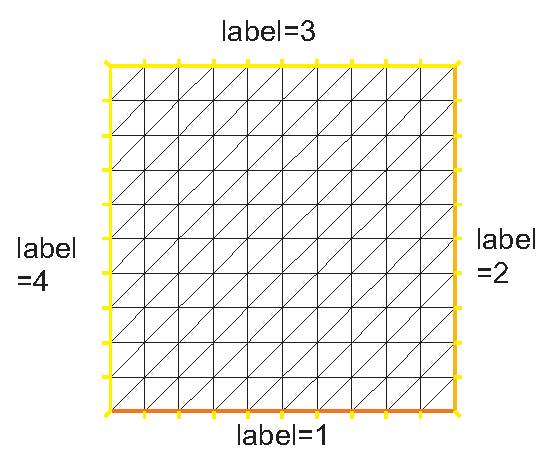
\includegraphics[height=5cm]{figures/square}
\end{center}
  \caption{Boundary labels of the mesh by \texttt{square(10,10)}}
  \label{fig:square} \index{label}
\end{figure}
If you want to construct a
$n\times m$ grid in the rectangle $[x_0,x_1]\times [y_0,y_1]$, you can
write
\bFF
  @real x0=1.2,x1=1.8;
  @real y0=0,y1=1;
  @int n=5,m=20;
  @mesh Th=@square(n,m,[x0+(x1-x0)*x,y0+(y1-y0)*y]);
\eFF
 \begin{note}
Adding the  parameter \texttt{flags=1}, will produce a
Union Jack flag type of mesh. \index{square!flags=}
\bFF
  @mesh Th=@square(n,m,[x0+(x1-x0)*x,y0+(y1-y0)*y],flags=1);
\eFF
\end{note}



\subsubsection{\setS{Border}}\index{border}\index{label}

A domain is defined as being on the left (resp right) of its
parameterized boundary
$$
\Gamma_j=\{(x,y)\left|\; x=\varphi_x(t),\, y=\varphi_y(t),\, a_j\le t\le b_j\right.\}
$$
We can easily check the orientation by drawing the curve
$t\mapsto (\varphi_x(t),\varphi_y(t)),\, t_0\le t\le t_1$.
If it is as in Fig. \ref{fig:border}, then
the domain lie on the shaded area, otherwise it lies on the opposite side

The boundaries $\Gamma_j$ can only intersect at their end points.

\begin{figure}[htbp]
\begin{center}
  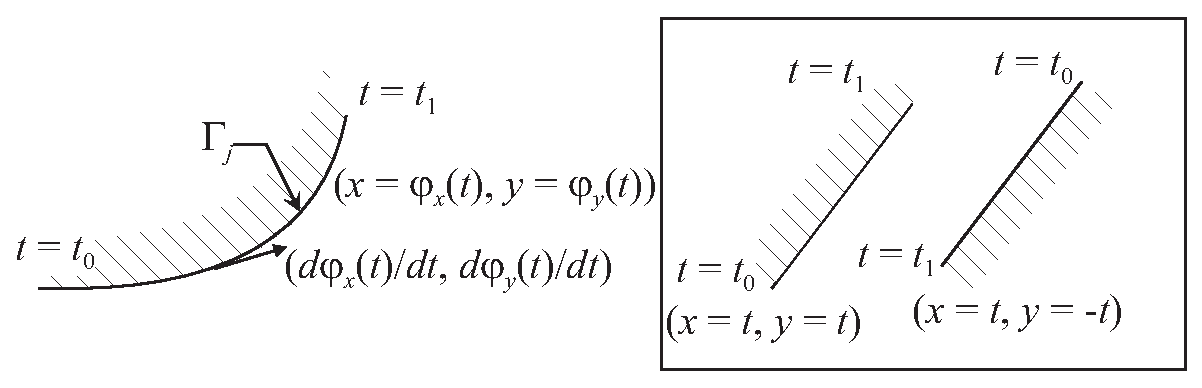
\includegraphics[height=4cm]{figures/border}
\end{center}
  \caption{Orientation of the boundary defined by $(\phi_x(t),\phi_y(t))$}
  \label{fig:border} \index{border}
\end{figure}
The general expression to define a triangulation with \texttt{buildmesh} is
\[
\ttCC{@mesh  ~~Mesh\_Name = @buildmesh$\left(\Gamma_1(m_1)+\cdots+\Gamma_J(m_j)\right)$;}
\]
where $m_j$ are positive or negative numbers to indicate how may point should be put on $\Gamma_j,\,
\Gamma=\cup_{j=1}^J \Gamma_J$.
We can change the orientation of boundaries by changing the sign of $m_j$.
The following example shows how to change the orientation.
The example generates the unit disk
with a small circular hole, and assign ``1'' to the unit disk
(``2'' to the circle inside).
The boundary label must be non-zero, but it can also be omitted.

\bFF
1: @border a(t=0,2*pi){ x=cos(t); y=sin(t);label=1;}
2: @border b(t=0,2*pi){ x=0.3+0.3*cos(t); y=0.3*sin(t);label=2;}
3: @plot(a(50)+b(+30)) ; // to see a plot of the border mesh \index{plot!border}
4: @mesh Thwithouthole= @buildmesh(a(50)+b(+30));
5: @mesh Thwithhole   = @buildmesh(a(50)+b(-30));
6: @plot(Thwithouthole,wait=1,ps="Thwithouthole.eps"); //figure \ref{Thwithouthole}\index{plot!mesh}
7: @plot(Thwithhole,wait=1,ps="Thwithhole.eps"); // figure \ref{Thwithhole}
\eFF
\begin{note}
You must notice that the orientation is changed by ``\texttt{b(-30)}'' in 5th line. In 7th line, \texttt{ps="fileName"} is used to generate a postscript file
identification that is shown on screen.
\end{note}

\twoplot[height=6cm]{Thwithouthole}{Thwithhole}{mesh without hole}{mesh with hole}

\subsubsection{Data Structure and Read/Write Statements for a Mesh}

\index{readmesh}\index{savemesh}
Users who want to use a triangulation made elsewhere should see the file structure
of the file generated below:
\bFF
@border C(t=0,2*pi) { x=cos(t); y=sin(t); }
@mesh Th = @buildmesh(C(10));
@savemesh("mesh_sample.msh");
\eFF
the mesh is shown on Fig. \ref{fig:meshSample}.
\\\\
The informations about \texttt{Th} are save in the file ``mesh\_sample.msh''.
whose structure is shown on Table \ref{tab:meshSample}.
\\
There $n_v$ denotes
the number of vertices, $n_t$ number of triangles
and $n_s$ the number of edges on boundary.

For each vertex $q^i,\, i=1,\cdots,n_v$, we denote by $(q^i_x,q^i_y)$
the $x$-coordinate and $y$-coordinate.

Each triangle $T_k, k=1,\cdots,10$ has three vertices $q^{k_1},\, q^{k_2},\,q^{k_3}$
that are oriented counterclockwise.
The boundary consists of 10 lines $L_i,\, i=1,\cdots,10$ whose end points are
$q^{i_1},\, q^{i_2}$.

\begin{figure}[htbp]
\begin{minipage}{\textwidth}
\begin{minipage}{0.5\textwidth}
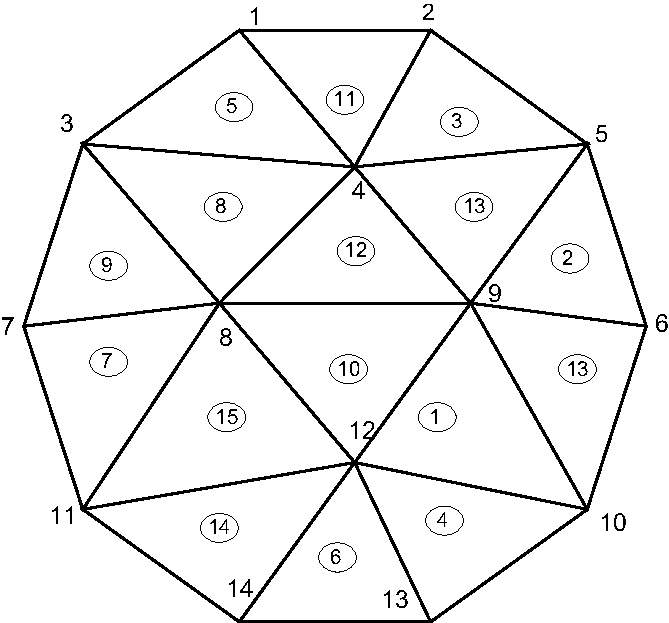
\includegraphics[width=\textwidth]{figures/mesh_sample}%
\caption{mesh by \texttt{buildmesh(C(10))}}
\label{fig:meshSample}
\end{minipage}
\hspace{0.5mm}
\begin{minipage}{0.5\textwidth}
In the left figure, we have the following.\\\\
$n_v=14,\, n_t=16,\, n_s=10$\\\\
$q^1=(-0.309016994375,\, 0.951056516295)$\\
$\vdots\qquad \vdots\qquad \vdots$\\
$q^{14}=(-0.309016994375,\, -0.951056516295)$\\\\
The vertices of $T_1$ are $q^9,\, q^{12},\, q^{10}$.\\
$\vdots\qquad \vdots\qquad \vdots$\\
The vertices of $T_{16}$ are $q^9,\, q^{10},\, q^{6}$.\\\\
The edge of 1st side $L_1$ are $q^6,\, q^5$.\\
$\vdots\qquad \vdots\qquad \vdots$\\
The edge of 10th side $L_{10}$ are $q^{10},\, q^6$.\\
\end{minipage}
\end{minipage}
\end{figure}

\begin{table}[htbp]
\begin{tabular}{|l|l|}
\hline
Contents of file&Explanation\\
\hline
14 16 10& $n_v$\qquad  $n_t$\qquad $n_e$\\
-0.309016994375 0.951056516295 1& $q^1_x$\qquad $q^1_y$\qquad boundary label=1\\
0.309016994375 0.951056516295 1& $q^2_x$\qquad $q^2_y$\qquad boundary label=1\\
$\cdots$  $\cdots$ $\vdots$& \\
-0.309016994375 -0.951056516295 1& $q^{14}_x$\qquad $q^{14}_y$\qquad boundary label=1\\
\hline
9 12 10 0&$1_1$\quad $1_2$\quad $1_3$\quad region label=0 \\
5 9 6 0&$2_1$\quad $2_2$\quad $2_3$\quad region label=0  \\
$\cdots$& \\
9 10 6 0&$16_1$\quad $16_2$\quad $16_3$\quad region label=0 \\
\hline
6 5 1&$1_1\quad 1_2$\quad boundary label=1\\
5 2 1&$2_1\quad 2_2$\quad boundary label=1\\
$\cdots$& \\
10 6 1&$10_1\quad 10_2$\quad boundary label=1\\
\hline
\end{tabular}
  \caption{The structure of ``mesh\_sample.msh''}
  \label{tab:meshSample}
\end{table}

There are many mesh file formats available for communication with
other tools such as emc2, modulef.. (see \refSec{Mesh Files}),
The extension of a file gives the chosen
type.\index{bamg} More details can be found in the article by F. Hecht
"bamg : a bidimentional anisotropic mesh generator" available from the
FreeFem web site.  \\
\\\\
 A
mesh file can be read back into \freefempp but the names of the
borders are lost. So these borders have to be referenced by the number
which corresponds to their order of appearance in the program, unless
this number is forced by the keyword "label".  Here are some examples:

\bFF
@border floor(t=0,1){ x=t; y=0; label=1;}; // the unit square
@border right(t=0,1){ x=1; y=t; label=5;};
@border ceiling(t=1,0){ x=t; y=1; label=5;};
@border left(t=1,0){ x=0; y=t; label=5;};
@int n=10;
@mesh th= buildmesh(floor(n)+right(n)+ceiling(n)+left(n));
@savemesh(th,"toto.am_fmt");  // "formatted Marrocco" format \index{file!am\_fmt}
@savemesh(th,"toto.Th");      // "bamg"-type mesh   \index{file!bamg}
@savemesh(th,"toto.msh");     // freefem format \index{file!mesh}
@savemesh(th,"toto.nopo");     // modulef format \index{file!nopo} see \cite{modulef}
@mesh th2 = readmesh("toto.msh"); // read the mesh

\eFF

The following example explains methods to obtain mesh information.
\index{triangle![]}\index{triangle!label}\index{triangle!label}
\index{vertex!x}\index{vertex!y}\index{vertex!label}
\bFF
{  // get mesh information (version 1.37)
  @mesh Th=square(2,2);
  // get data of the mesh
  @int nbtriangles=Th.nt;
  @for (@int i=0;i<nbtriangles;i++)
    @for (@int j=0; j <3; j++)
      @cout << i << " " << j << " Th[i][j] = "
           << Th[i][j] << "  x = "<< Th[i][j].x  << " , y= "<< Th[i][j].y
           << ",  label=" << Th[i][j].label << endl;

  // To this day:   this Hack works: to get x,y of vertex i \hfilll
  // remark: i can be set with i= Th[it][j] \hfilll
  // the idea is to build de interpolation of x and y function \hfilll
  // with 2 array now given i -> x and i-> y. \hfilll

  @fespace femp1(Th,P1);
  femp1 Thx=x,Thy=y;
  @cout << " nb of vertices = " << nbvertices << endl;
  @for (@int i=0;i<nbvertices;i++)
        @cout << i  << " : " << Thx[][i] << " " << Thy[][i] << endl;

  //Hack  to get a triangle number of mesh containing point x,y \hfilll
  //     or  region number \hfilll
  // ----------------------------------------- \hfilll
  @fespace femp0(Th,P0);
  femp0 nuT; // a P0 function  to get triangle numbering
    @for (@int i=0;i<Th.nt;i++)
     nuT[][i]=i;
  femp0 nuReg=region; // a P0 function to get the region number
  //  inquire
  @int it0=nuT(0.55,0.6); //  number of triangle containing point (0.55,0,6);
  @int nr0=nuReg(0.55,0.6); //  number of region of mesh containing point (0.55,0,6);
  // new method if   version > 1.450007
  @int it00 = Th(0.55,0.6).nuTriangle; // get the number of Th's triangle containing (0.55,0.6)
  @int nr00 = Th(0.55,0.6).region;; // get the region  number of Th's triangle
    // dump
  @cout << "  point (0.55,0,6) :triangle number " << it0 << " " << it00
       << ", region = " << nr0 << " == " << nr00 << endl;
}

\eFF
the output is:
\bFF
0 0 Th[i][j] = 0  x = 0 , y= 0,  label=4
0 1 Th[i][j] = 1  x = 0.5 , y= 0,  label=1
0 2 Th[i][j] = 4  x = 0.5 , y= 0.5,  label=0
1 0 Th[i][j] = 0  x = 0 , y= 0,  label=4
1 1 Th[i][j] = 4  x = 0.5 , y= 0.5,  label=0
1 2 Th[i][j] = 3  x = 0 , y= 0.5,  label=4
.......
5 2 Th[i][j] = 6  x = 0 , y= 1,  label=4
6 0 Th[i][j] = 4  x = 0.5 , y= 0.5,  label=0
6 1 Th[i][j] = 5  x = 1 , y= 0.5,  label=2
6 2 Th[i][j] = 8  x = 1 , y= 1,  label=3
7 0 Th[i][j] = 4  x = 0.5 , y= 0.5,  label=0
7 1 Th[i][j] = 8  x = 1 , y= 1,  label=3
7 2 Th[i][j] = 7  x = 0.5 , y= 1,  label=3
 Nb Of Nodes = 9
 Nb of DF = 9
 -- vector function's bound  -0 1
 -- vector function's bound  -0 1
 nb of vertices = 9
0 : -0 -0
1 : 0.5 -0
2 : 1 -0
3 : -0 0.5
4 : 0.5 0.5
5 : 1 0.5
6 : -0 1
7 : 0.5 1
8 : 1 1
 Nb Of Nodes = 8
 Nb of DF = 8
 -- vector function's bound  -0 -0
  point (0.55,0,6) :triangle number 7 7, region = 0 == 0
\eFF
\begin{example}[Readmesh.edp]
\index{tutorial!readmesh.edp}
\index{read files}
\index{write files}
\bFF

@border floor(t=0,1){ x=t; y=0; label=1;}; // the unit square
@border right(t=0,1){ x=1; y=t; label=5;};
@border ceiling(t=1,0){ x=t; y=1; label=5;};
@border left(t=1,0){ x=0; y=t; label=5;};
@int n=10;
@mesh th= buildmesh(floor(n)+right(n)+ceiling(n)+left(n));
@savemesh(th,"toto.am_fmt");  // format "formated Marrocco" \index{file!am\_fmt}
@savemesh(th,"toto.Th");      // format database  db mesh "bamg"   \index{file!bamg}
@savemesh(th,"toto.msh");     // format freefem \index{file!mesh}
@savemesh(th,"toto.nopo");     // modulef format \index{file!nopo} see \cite{modulef}
@mesh th2 = readmesh("toto.msh");
@fespace femp1(th,@P1);
femp1 f = sin(x)*cos(y),g;
{ // save solution
@ofstream file("f.txt");
file << f[] << endl;
}  // close the file (end block)
{  // read
@ifstream file("f.txt");
file >> g[] ;
} // close reading file (end block)
@fespace Vh2(th2,P1);
Vh2 u,v;
@plot(g);
//  find $u$ such that \hfilll
// $ u - \Delta u = g $ in $\Omega $ , \hfilll
// $ u=0$ on $\Gamma_1$ and $\frac{\p u }{\p n} = g$ on $\Gamma_2$  \hfilll
@solve pb(u,v) =
    @int2d(th)( u*v - dx(u)*dx(v)-dy(u)*dy(v) )
  + @int2d(th)(-g*v)
  + @int1d(th,5)( g*v) //  $\frac{\p u }{\p n} = g$ on $\Gamma_2$
  + @on(1,u=0) ;
@plot (th2,u);
\eFF
\end{example}

\subsubsection{The keyword "triangulate"}\index{triangulate}

\freefempp is able to build a triangulation from a set of points. This
triangulation is a Delaunay mesh of the convex hull of the set of points.
It can be useful to build a mesh form a table function.

The coordinates of the points and the value of the table function
are defined separately with rows of the form: \texttt{x y f(x,y)}
in a file such as:

\bFF
0.51387 0.175741 0.636237
0.308652 0.534534 0.746765
0.947628 0.171736 0.899823
0.702231 0.226431 0.800819
0.494773 0.12472 0.580623
0.0838988 0.389647 0.456045
...............
\eFF
%%% Thxy.eps not found
\twoplot[height=4cm]{Thxy}{xyf}{Delaunay mesh of the convex hull of point set in file xyf}
{Isovalue of table function}

The third column of each line is left untouched by the
\texttt{triangulate} command. But you can use this third value to
define a table function with rows of the form: \texttt{x y f(x,y)}.


The following example shows how to make a mesh from the file ``xyf''
with the format stated just above.
The command
\texttt{triangulate} command use only use 1st and 2nd rows.

\index{function!tables}

\bFF
@mesh Thxy=@triangulate("xyf"); // build the Delaunay mesh of the convex hull
// points are defined by the first 2 columns of file \texttt{xyf}
@plot(Thxy,ps="Thxyf.ps"); // (see figure  \ref{Thxy})

@fespace Vhxy(Thxy,P1); // create a P1 interpolation
Vhxy fxy; // the function

// reading the 3rd row to define the function
{ @ifstream file("xyf");
   @real xx,yy;
   @for(@int i=0;i<fxy.n;i++)
   file >> xx >>yy >> fxy[][i];  // to read third row only.
   // xx and yy are just skipped
}
@plot(fxu,ps="xyf.eps"); // plot the function (see figure  \ref{xyf})
\eFF

\subsection{Boundary FEM Spaces Built as Empty Meshes}\index{emptymesh}
To define a Finite Element space on boundary,
we came up with the idea of a mesh with no internal points (call empty mesh).
It can be useful when you have a Lagrange multiplier definied on the border.

So the function emptymesh remove all the internal points of a mesh except
points is on  internal boundaries.

\bFF
{  //  new stuff 2004 emptymesh (version 1.40)
 // -- useful to build Multiplicator space
 //  build a mesh without internal point
 // with the same boundary
 //  -----
  assert(version>=1.40);
  @border a(t=0,2*pi){ x=cos(t); y=sin(t);label=1;}
  @mesh Th=buildmesh(a(20));
   Th=@emptymesh(Th);
  @plot(Th,wait=1,ps="emptymesh-1.eps");//see figure \ref{fig emptymesh-1}
}
\eFF

It is also possible to build an empty mesh of a pseudo subregion
with \texttt{emptymesh(Th,ssd)} with the set of edges of the mesh \texttt{Th};
a edge $e$ is in  this set  if with the two adjacent triangles $e =t1\cap t2$
and  $ ssd[T1] \neq ssd[T2]$ where \texttt{ssd}  refers to the pseudo region
numbering of triangles, when they are stored in an \texttt{int[int]} array of size the number of triangles.
\bFF
{  //  new stuff 2004 emptymesh (version 1.40) \hfilll
 // -- useful to build Multiplicator space \hfilll
 //  build a mesh without internal point \hfilll
 // of peusdo sub domain  \hfilll
 //  ----- \hfilll
  @assert(version>=1.40);
  @mesh Th=@square(10,10);
  @int[@int] ssd(Th.nt);
  @for(@int i=0;i<ssd.n;i++) // build the  pseudo region numbering
   {  @int iq=i/2;   // because 2 triangle per quad
      @int ix=iq%10; //
      @int iy=iq/10; //
    ssd[i]= 1 + (ix>=5) +  (iy>=5)*2;
   }
  Th=@emptymesh(Th,ssd); // build emtpy  with
  //  all edge $e = T1 \cap T2$ and $ ssd[T1] \neq ssd[T2]$
  @plot(Th,wait=1,ps="emptymesh-2.eps");//see figure \ref{fig emptymesh-2}
  @savemesh(Th,"emptymesh-2.msh");
}
\eFF

\twoplot[height=6cm]{emptymesh-1}{emptymesh-2}{ The empty mesh with boundary
\label{fig emptymesh-1}}{An empty mesh
defined from a pseudo region numbering of triangle\label{fig emptymesh-2}}

\subsection{Remeshing}
\subsubsection{\setS{Movemesh}}\index{movemesh}\index{checkmovemesh}

Meshes can be translated, rotated and deformed by {\tt movemesh}; this is useful for
 elasticity to watch the deformation due to the displacement
$\vec\Phi(x,y)=(\Phi_1(x,y),\Phi_2(x,y))$ of shape. It is also useful to
handle free boundary  problems or optimal shape problems.

If $\Omega$ is triangulated as $T_h(\Omega)$,
and $\Phi$ is a displacement vector then $\Phi(T_h)$ is obtained by
\bFF
@mesh  Th=@movemesh(Th,[$\Phi$1,$\Phi$2]);
\eFF
Sometimes the moved mesh is invalid because some triangle
becomes reversed (with a negative area). This is why we should check the
minimum triangle area in the transformed mesh with
\texttt{checkmovemesh} before any real transformation.

\begin{example} $\Phi_1(x,y)=x+k*\sin(y*\pi)/10)$,
$\Phi_2(x,y)=y+k*\cos(y\pi)/10)$ for a big number $k>1$.
\bFF
verbosity=4;
@border a(t=0,1){x=t;y=0;label=1;};
@border b(t=0,0.5){x=1;y=t;label=1;};
@border c(t=0,0.5){x=1-t;y=0.5;label=1;};
@border d(t=0.5,1){x=0.5;y=t;label=1;};
@border e(t=0.5,1){x=1-t;y=1;label=1;};
@border f(t=0,1){x=0;y=1-t;label=1;};
@func uu= sin(y*pi)/10;
@func vv= cos(x*pi)/10;

@mesh Th = buildmesh ( a(6) + b(4) + c(4) +d(4) + e(4) + f(6));
@plot(Th,wait=1,fill=1,ps="Lshape.eps");// see figure \ref{lshape}
@real coef=1;
@real minT0= @checkmovemesh(Th,[x,y]); // the min triangle area
@while(1) // find a correct move mesh
{
  @real minT=@checkmovemesh(Th,[x+coef*uu,y+coef*vv]);//the min triangle area
  if (minT > minT0/5) break ; // if big enough
  coef=/1.5;
}

Th=@movemesh(Th,[x+coef*uu,y+coef*vv]);
@plot(Th,wait=1,fill=1,ps="movemesh.eps");// see figure \ref{movemesh}
\eFF

\twoplot[height=6cm]{lshape}{movemesh}{L-shape}{  moved L-shape }
\end{example}
\begin{note}
Consider a function $u$ defined on a mesh \texttt{Th}. A statement like
\texttt{Th=movemesh(Th...)} does not change $u$ and so the old mesh
still exists. It will be destroyed when no function use it. A
statement like $u=u$ redefines $u$ on the new mesh \texttt{Th} with
interpolation and therefore destroys the old \texttt{Th} if $u$ was the only
function using it.
\end{note}

\begin{example}[movemesh.edp]
\index{tutorial!movemesh.edp}
Now, we given an example of moving mesh with a lagrangian\index{lagrangian}
function $u$ defined on the moving mesh.

\bFF
// simple movemesh example
@mesh Th=square(10,10);
@fespace Vh(Th,P1);
@real t=0;
// ---
//  the problem is how to build data without interpolation
//  so the data u is moving with the mesh as you can see in the plot
// ---
Vh u=y;
@for (int i=0;i<4;i++)
{
 t=i*0.1;
 Vh f= x*t;
 @real minarea=checkmovemesh(Th,[x,y+f]);
 if (minarea >0 ) // movemesh will be ok
   Th=movemesh(Th,[x,y+f]);

 cout << " Min area  " << minarea << endl;

 real[int] tmp(u[].n);
 tmp=u[];  // save the value
 u=0;        // to change the FEspace and mesh associated with u
 u[]=tmp;  // set the value of u without any mesh update
 @plot(Th,u,wait=1);
};
// In this program, since u is only defined on the last mesh, all the \hfilll
// previous meshes are deleted from memory.  \hfilll
//   --------  \hfilll
\eFF
\end{example}

\subsection{\setS{Regular Triangulation}: {\tt hTriangle}}
For a set $S$, we define the diameter of $S$ by
\[
\textrm{diam}(S)=\sup\{|\vec{x}-\vec{y}|; \; \vec{x},\, \vec{y}\in S\}
\]
The sequence $\{\mathcal{T}_h\}_{h\downarrow 0}$ of $\Omega$ is called
\emph{regular}\index{mesh!regular} if they satisfy the following:
\begin{enumerate}
  \item
\[
\lim_{h\downarrow 0}\max\{\textrm{diam}(T_k)|\; T_k\in \mathcal{T}_h\}=0
\]
  \item
There is a number $\sigma>0$ independent of $h$ such that
\[
\frac{\rho(T_k)}{\textrm{diam}(T_k)}\ge \sigma
\qquad \textrm{for all }T_k\in \mathcal{T}_h
\]
where $\rho(T_k)$ are the diameter of the inscribed circle of $T_k$.
\end{enumerate}
We put $h(\mathcal{T}_h)=\max\{\textrm{diam}(T_k)|\; T_k\in \mathcal{T}_h\}$,
which is obtained by
\bFF
@mesh Th = ......;
@fespace Ph(Th,P0);
Ph h = @hTriangle;
@cout << "size of mesh = " << h[].max << @endl;
\eFF

\subsection{Adaptmesh}\index{adaptmesh}
\label{sec:Adaptmesh}
The function
\[
f(x,y) = 10.0x^3+y^3+\tan^{-1}[\epsilon/(\sin(5.0y)-2.0x)]
\qquad \epsilon =  0.0001
\]
sharply varies in value.
However, the initial mesh given by the command in Section \ref{sec:InitialMesh}
cannot reflect its sharp variations.
\begin{example}~
\bFF
@real eps =  0.0001;
@real h=1;
@real hmin=0.05;
@func f = 10.0*x^3+y^3+h*atan2(eps,sin(5.0*y)-2.0*x);

@mesh Th=square(5,5,[-1+2*x,-1+2*y]);
@fespace Vh(Th,P1);
Vh fh=f;
@plot(fh);
for (@int i=0;i<2;i++)
 {
   Th=@adaptmesh(Th,fh);
   fh=f;  // old mesh is deleted
   @plot(Th,fh,wait=1);
 }
\eFF
\end{example}
\plot[height=10cm]{adaptmesh}{3D graphs for the initial mesh and 1st and 2nd mesh adaptation}

\freefempp uses a variable metric/Delaunay automatic meshing
algorithm.
The command
\bFF
@mesh ATh = @adaptmesh(Th, f);
\eFF
create the new mesh \texttt{ATh} by the Hessian
$$
D^2f=(\p^2 f/\p x^2,\, \p^2 f/\p x\p y,
\p^2 f/\p y^2)
$$
of a function (formula or FE-function).
Mesh adaptation is a very powerful tool when the solution of a problem
vary locally and sharply.

Here we solve the problem (\ref{eqn:Poisson})-(\ref{eqn:Dirichlet}),
when $f=1$ and $\Omega$ is a L-shape domain.

\twoplot[height=5cm]{L-shape2}{lshapeSol}{ L-shape domain and its boundary name}{Final solution after 4-times adaptation}


\begin{example}[Adapt.edp]
\index{tutorial!adapt.edp}
The solution has the
\index{singularity}singularity $r^{3/2},\, r=|x-\gamma|$
at the point $\gamma$ of the intersection of two lines
$bc$ and $bd$ (see Fig. \ref{L-shape2}).
\bFF
@border ba(t=0,1.0){x=t;   y=0;  label=1;};
@border bb(t=0,0.5){x=1;   y=t;  label=1;};
@border bc(t=0,0.5){x=1-t; y=0.5;label=1;};
@border bd(t=0.5,1){x=0.5; y=t;  label=1;};
@border be(t=0.5,1){x=1-t; y=1;  label=1;};
@border bf(t=0.0,1){x=0;   y=1-t;label=1;};
@mesh Th = @buildmesh ( ba(6)+bb(4)+bc(4)+bd(4)+be(4)+bf(6) );
@fespace Vh(Th,@P1);  // set FE space
Vh u,v;             // set unknown and test function
func f = 1;
@real error=0.1;        // level of error
@problem Poisson(u,v,solver=CG,eps=1.0e-6) =
    @int2d(Th)(  dx(u)*dx(v) + dy(u)*dy(v))
  - @int2d(Th) ( f*v )
  + @on(1,u=0)  ;
@for (@int i=0;i< 4;i++)
{
  Poisson;
  Th=@adaptmesh(Th,u,err=error);
  error = error/2;
} ;
@plot(u);
\eFF
\end{example}
To speed up the adaptation
we change by hand a default parameter \texttt{err} of
\texttt{adaptmesh}\index{concatenation}, which
specifies the required precision, so as to make the new mesh finer.
The problem is coercive and symmetric,
so the linear system can be solved with the conjugate gradient
method \index{solver=!CG} (parameter \texttt{solver=CG}
with the stopping criteria on the residual, here
\texttt{eps=1.0e-6}).
By \texttt{adaptmesh}, we get good slope of the final solution near
the point of intersection of $bc$ and $bd$ as in Fig. \ref{lshapeSol}.

This method is described in detail in \cite{bamg}. It has a number of
default parameters which can be modified~:

\index{adaptmesh}
\begin{description}

    \item[\texttt{hmin=}] Minimum edge size.  \index{adaptmesh!hmin=}
    ({\tt val} is a real. Its default is related to
    the size of the domain to be meshed and the precision of the mesh
    generator).

    \item[\texttt{hmax=}] Maximum edge size.  ({\tt val} is a real.
    It defaults to the diameter of the domain to be
    meshed) \index{adaptmesh!hmax=}

    \item[\texttt{err=}] $P^1$ interpolation error level (0.01 is the
    default).  \index{adaptmesh!err=}

    \item[\texttt{errg=}] Relative geometrical error. By default this
    error is 0.01, and in any case it must be lower than $1/\sqrt{2}$.
    Meshes created with this option may have some edges smaller than
    the {\tt -hmin } due to geometrical constraints.
    \index{adaptmesh!errg=}

    \item[\texttt{nbvx=}] Maximum number of vertices generated by the
    mesh generator (9000 is the default).
    \index{adaptmesh!nbvx=}

    \item[\texttt{nbsmooth=}] number of iterations of the smoothing
    procedure (5 is the default).  \index{adaptmesh!nbsmooth=}

    \item[\texttt{nbjacoby=}] number of iterations in a smoothing
    procedure during the metric construction, 0 means no smoothing (6
    is the default).  \index{adaptmesh!nbjacoby=}

    \item[\texttt{ratio=}] ratio for a prescribed smoothing on the
    metric.  If the value is 0 or less than 1.1 no smoothing is done
    on the metric (1.8 is the default).

    If \texttt{ratio} $> 1.1$, the speed of mesh size variations is
    bounded by $log(\mathtt{ratio})$.  Note: As {\tt ratio} gets
    closer to {\tt 1}, the number of generated vertices increases.
    This may be useful to control the thickness of refined regions
    near shocks or boundary layers .  \index{adaptmesh!ratio=}

   \item[\texttt{omega=}] relaxation parameter for the smoothing
   procedure (1.0 is the default).  \index{adaptmesh!omega=}

    \item[\texttt{iso=}] If true, forces the metric to be isotropic
    (false is the default).  \index{adaptmesh!iso=}

    \item[\texttt{abserror=}] If false, the metric is evaluated using
    the criterium of equi-repartion of relative error (false is the
    default).  In this case the metric is defined by

\begin{equation}
  \mathcal{M} = \left({1\over\mathtt{err}\,\, \mathtt{coef}^2} \quad {
  |\mathcal{H}| \over max(\mathtt{CutOff},|\eta|)}\right)^p
  \label{eq err rel}
\end{equation}
    \index{adaptmesh!abserror=}

    otherwise, the metric is evaluated using the criterium of
    equi-distribution of errors.  In this case the metric is defined
    by

\begin{equation}
  \mathcal{M} = \left({1\over \mathtt{err}\,\,\mathtt{coef}^2} \quad
  {|{\mathcal{H}|} \over
  {\mathit{sup}(\eta)-\mathit{inf}(\eta)}}\right)^p.\label{eq err abs}
\end{equation}

    \item[\texttt{cutoff=}] lower limit for the relative error
    evaluation (1.0e-6 is the default).
    \index{adaptmesh!cutoff=}

    \item[\texttt{verbosity=}] informational messages level (can be
    chosen between 0 and $\infty$). Also changes the value of the
    global variable verbosity (obsolete).  \index{adaptmesh!verbosity=
    }

    \item[\texttt{inquire=}] To inquire graphically about the mesh (false is the
    default).  \index{adaptmesh!inquire=}

    \item[\texttt{splitpbedge=}] If true, splits all internal edges in
    half with two boundary vertices (true is the default).
    \index{adaptmesh!splitpbedge=}

    \item[\texttt{maxsubdiv=}] Changes the metric such that the
    maximum subdivision of a background edge is bound by {\tt val}
    (always limited by 10, and 10 is also the default).
    \index{adaptmesh!maxsubdiv=}

    \item[\texttt{rescaling=}] if true, the function with respect to
    which the mesh is adapted is rescaled to be between 0 and 1 (true
    is the default).  \index{adaptmesh!rescaling=}

    \item[\texttt{keepbackvertices=}] if true, tries to keep as many
    vertices from the original mesh as possible (true is the default).
    \index{adaptmesh!keepbackvertices=}

    \item[\texttt{isMetric=}] if true, the metric is defined
    explicitly (false is the default).  If the 3 functions $m_{11},
    m_{12}, m_{22}$ are given, they directly define a symmetric matrix
    field whose Hessian is computed to define a metric. If only one
    function is given, then it represents the isotropic mesh size at
    every point.  \index{adaptmesh!isMetric=}

    For example, if the partial derivatives
    \texttt{fxx} ($=\p^2 f/\p x^2$),
    \texttt{fxx} ($=\p^2 f/\p x\p y$),
    \texttt{fyy} ($=\p^2 f/\p y^2$) are given, we can set
    $$
    \ttCC{Th=@adaptmesh(Th,fxx,fxy,fyy,IsMetric=1,nbvx=10000,hmin=hmin);}
    $$

    \item[\texttt{power=}] exponent power of the Hessian used to
    compute the metric (1 is the default).  \index{adaptmesh!powerin=}

    \item[\texttt{thetamax=}] minimum corner angle in degrees (default
    is 0).

    \item[\texttt{splitin2=}] boolean value. If true, splits all
    triangles of the final mesh into 4
    sub-triangles. \index{adaptmesh!splitin2}

    \item[\texttt{metric=}] \index{adaptmesh!metric=} an array of 3
    real arrays to set or get metric data information. The size of
    these three arrays must be the number of vertices. So if
    \texttt{m11,m12,m22} are three P1 finite elements related to the
    mesh to adapt, you can write: \texttt{metric=[m11[],m12[],m22[]]}
    (see file convect-apt.edp for a full example)

    \itemtt[nomeshgeneration=] \index{adaptmesh!nomeshgeneration=} If
    true, no adapted mesh is generated (useful to compute only a
    metric).

    \itemtt[periodic=] \index{adaptmesh!periodic=} %%% modif FH
    As writing \texttt{periodic=[[4,y],[2,y],[1,x],[3,x]];}
    it builds an adapted periodic mesh. The sample
    build a biperiodic mesh of a square.
    (see periodic finite element   spaces \ref{periodic BC}, and see \texttt{sphere.edp} for a  full example)

\end{description}

%%%alh proofreading ok up to here

\subsection{Trunc}\index{trunc}

Two operators have been introduce to remove triangles from a mesh or to divide them.
Operator {\tt trunc } has two parameters
\begin{description} \index{split=} \index{label=}\index{trunc!split=} \index{trunc!label=}
  \itemtt[label=] sets the label number of new boundary item (one by default)
  \itemtt[split=] sets the level $n$ of triangle splitting. each triangle is splitted in  $n\times n$ ( one by default).
\end{description}

To create the mesh \texttt{Th3}
where alls  triangles of a mesh \texttt{Th}  are splitted in $3{\times}3$ , just write:
\bFF
  mesh Th3 = trunc(Th,1,split=3);
\eFF

The  \texttt{truncmesh.edp} example construct
all "trunc" mesh  to the support of the basic function  of the space \texttt{Vh} (cf. \texttt{abs(u)>0}),
split all the  triangles in $5{\times} 5$, and put a label number to $2$ on new boundary.
\bFF
@mesh Th=square(3,3);
@fespace Vh(Th,P1);
Vh u;
@int i,n=u.n;
u=0;
@for (i=0;i<n;i++)  // all degree of freedom
 {
  u[][i]=1;        //  the basic function i
  @plot(u,wait=1);
  @mesh Sh1=trunc(Th,abs(u)>1.e-10,split=5,label=2);
  plot(Th,Sh1,wait=1,ps="trunc"+i+".eps");// plot the mesh of
  // the function's support
  u[][i]=0;      // reset
 }
\eFF
\twoplot[height=6cm]{trunc0}{trunc6}{ mesh of support the function P1  number 0, splitted in $5{\times}5$ }{
mesh of support the function P1  number 6, splitted in $5{\times}5$ }
\subsection{Splitmesh}
Another way to split mesh triangles is to use {\tt splitmesh}, for example:
\bFF
{  //  new stuff 2004 splitmesh (version 1.37)
  assert(version>=1.37);
  @border a(t=0,2*pi){ x=cos(t); y=sin(t);label=1;}
  @plot(Th,wait=1,ps="nosplitmesh.eps"); // see figure \ref{fig nosplitmesh}
  @mesh Th=@buildmesh(a(20));
  @plot(Th,wait=1);
  @Th=@splitmesh(Th,1+5*(square(x-0.5)+y*y));
  @plot(Th,wait=1,ps="splitmesh.eps"); // see figure \ref{fig splitmesh}
}
\eFF

\twoplot[height=6cm]{nosplitmesh}{splitmesh}{\label{fig nosplitmesh}initial mesh}{\label{fig splitmesh}all left mesh triangle is split  conformaly in \texttt{int(1+5*(square(x-0.5)+y*y)\^2} triangles.}


\subsection{\setS{Meshing Examples}}

\begin{example}[Two rectangles touching by a side]~
\index{mesh!beam}
\bFF
@border a(t=0,1){x=t;y=0;};
@border b(t=0,1){x=1;y=t;};
@border c(t=1,0){x=t ;y=1;};
@border d(t=1,0){x = 0; y=t;};
@border c1(t=0,1){x=t ;y=1;};
@border e(t=0,0.2){x=1;y=1+t;};
@border f(t=1,0){x=t ;y=1.2;};
@border g(t=0.2,0){x=0;y=1+t;};
@int n=1;
@mesh th = @buildmesh(a(10*n)+b(10*n)+c(10*n)+d(10*n));
@mesh TH = @buildmesh ( c1(10*n) + e(5*n) + f(10*n) + g(5*n) );
@plot(th,TH,ps="TouchSide.esp"); // Fig. \ref{TouchSide}
\eFF
\end{example}

\begin{example}[NACA0012 Airfoil]~
\index{mesh!NACA0012}
\bFF
@border upper(t=0,1) { x = t;
     y = 0.17735*sqrt(t)-0.075597*t
  - 0.212836*(t^2)+0.17363*(t^3)-0.06254*(t^4); }
@border lower(t=1,0) { x = t;
     y= -(0.17735*sqrt(t)-0.075597*t
  -0.212836*(t^2)+0.17363*(t^3)-0.06254*(t^4)); }
@border c(t=0,2*pi) { x=0.8*cos(t)+0.5;  y=0.8*sin(t); }
@mesh Th = @buildmesh(c(30)+upper(35)+lower(35));
@plot(Th,@ps="NACA0012.eps",@bw=1);  // Fig. \ref{NACA0012}
\eFF
\end{example}

\twoplot[height=5cm]{TouchSide}{NACA0012}{Two rectangles touching by a side}
{NACA0012 Airfoil}

\begin{example}[Cardioid]~
\index{mesh!Cardioid}
\bFF
@real b = 1, a = b;
@border C(t=0,2*pi) { x=(a+b)*cos(t)-b*cos((a+b)*t/b);
                        y=(a+b)*sin(t)-b*sin((a+b)*t/b); }
@mesh Th = @buildmesh(C(50));
@plot(Th,@ps="Cardioid.eps",bw=1); // Fig. \ref{Cardioid}
\eFF
\end{example}
\begin{example}[Cassini Egg]~
\index{mesh!Cassini Egg}
\bFF
@border C(t=0,2*pi) { x=(2*cos(2*t)+3)*cos(t);
                      y=(2*cos(2*t)+3)*sin(t); }
@mesh Th = @buildmesh(C(50));
@plot(Th,@ps="Cassini.eps",bw=1); // Fig. \ref{Cassini}
\eFF
\end{example}
\twoplot[height=5cm]{Cardioid}{Cassini}{Domain with Cardioid curve boundary}
{Domain with Cassini Egg curve boundary}

\begin{example}[By cubic Bezier curve]~
\index{mesh!Bezier curve}
\bFF
// A cubic Bezier curve connecting two points with two control points
@func @real @bzi(@real p0,@real p1,@real q1,@real q2,@real t)
{
  @return p0*(1-t)^3+q1*3*(1-t)^2*t+q2*3*(1-t)*t^2+p1*t^3;
}

real[int] p00=[0,1], p01=[0,-1], q00=[-2,0.1], q01=[-2,-0.5];
real[int] p11=[1,-0.9], q10=[0.1,-0.95], q11=[0.5,-1];
real[int] p21=[2,0.7], q20=[3,-0.4], q21=[4,0.5];
real[int] q30=[0.5,1.1], q31=[1.5,1.2];
@border G1(t=0,1) { x=bzi(p00[0],p01[0],q00[0],q01[0],t);
                   y=bzi(p00[1],p01[1],q00[1],q01[1],t); }
@border G2(t=0,1) { x=bzi(p01[0],p11[0],q10[0],q11[0],t);
                   y=bzi(p01[1],p11[1],q10[1],q11[1],t); }
@border G3(t=0,1) { x=bzi(p11[0],p21[0],q20[0],q21[0],t);
                   y=bzi(p11[1],p21[1],q20[1],q21[1],t); }
@border G4(t=0,1) { x=bzi(p21[0],p00[0],q30[0],q31[0],t);
                   y=bzi(p21[1],p00[1],q30[1],q31[1],t); }
@int m=5;
@mesh Th = @buildmesh(G1(2*m)+G2(m)+G3(3*m)+G4(m));
@plot(Th,ps="Bezier.eps",bw=1);  // Fig \ref{Bezier}
\eFF
\end{example}

\begin{example}[Section of Engine]~
\index{mesh!Section of Engine}
\bFF
real a= 6., b= 1., c=0.5;
border L1(t=0,1) { x= -a; y= 1+b - 2*(1+b)*t; }
border L2(t=0,1) { x= -a+2*a*t; y= -1-b*(x/a)*(x/a)*(3-2*abs(x)/a );}
border L3(t=0,1) { x= a; y=-1-b + (1+ b )*t; }
border L4(t=0,1) { x= a - a*t;   y=0; }
border L5(t=0,pi) { x= -c*sin(t)/2; y=c/2-c*cos(t)/2; }
border L6(t=0,1) { x= a*t;  y=c; }
border L7(t=0,1) { x= a;  y=c + (1+ b-c )*t; }
border L8(t=0,1) { x= a-2*a*t; y= 1+b*(x/a)*(x/a)*(3-2*abs(x)/a); }
mesh Th = buildmesh(L1(8)+L2(26)+L3(8)+L4(20)+L5(8)+L6(30)+L7(8)+L8(30));
plot(Th,ps="Engine.eps",bw=1); // Fig. \ref{Engine}
\eFF
\end{example}

\begin{figure}[hbt]
\begin{multicols}{2}
\begin{center}
\includegraphics*[height=5cm]{Bezier}
\caption{\label{Bezier} Boundary drawed by Bezier curves}
\end{center}
\begin{center}
\vspace{3cm}~~\\
\includegraphics*[height=2.8cm]{Engine}
\caption{\label{Engine} Section of Engine}
\end{center}
\end{multicols}
\end{figure}

\begin{example}[Domain with U-shape channel]~
\index{mesh!U-shape channel}
\bFF
@real d = 0.1; // width of U-shape
@border L1(t=0,1-d) { x=-1; y=-d-t; }
@border L2(t=0,1-d) { x=-1; y=1-t; }
@border B(t=0,2) { x=-1+t; y=-1; }
@border C1(t=0,1) { x=t-1; y=d; }
@border C2(t=0,2*d) { x=0; y=d-t; }
@border C3(t=0,1) { x=-t; y=-d; }
@border R(t=0,2) { x=1; y=-1+t; }
@border T(t=0,2) { x=1-t; y=1; }
@int n = 5;
@mesh Th = buildmesh (L1(n/2)+L2(n/2)+B(n)+C1(n)+C2(3)+C3(n)+R(n)+T(n));
@plot(Th,ps="U-shape.eps",bw=1); // Fig \ref{U-shape}
\eFF
\end{example}
\begin{example}[Domain with V-shape cut]~
\index{mesh!V-shape cut}
\bFF
@real dAg = 0.01; // angle of V-shape
@border C(t=dAg,2*pi-dAg) { x=cos(t); y=sin(t); };
@real[int] pa(2), pb(2), pc(2);
pa[0] = cos(dAg); pa[1] = sin(dAg);
pb[0] = cos(2*pi-dAg); pb[1] = sin(2*pi-dAg);
pc[0] = 0; pc[1] = 0;
@border seg1(t=0,1) { x=(1-t)*pb[0]+t*pc[0]; y=(1-t)*pb[1]+t*pc[1]; };
@border seg2(t=0,1) { x=(1-t)*pc[0]+t*pa[0]; y=(1-t)*pc[1]+t*pa[1]; };
@mesh Th = @buildmesh(seg1(20)+C(40)+seg2(20));
@plot(Th,@ps="V-shape.eps",@bw=1);  // Fig. \ref{V-shape}
\eFF
\end{example}
\twoplot[height=5cm]{U-shape}{V-shape}{Domain with U-shape channel changed by \ttCC{d}}
{Domain with V-shape cut changed by \ttCC{dAg}}

\begin{example}[Smiling face]~
\index{mesh!Smiling face}
\bFF
@real d=0.1;
@int m=5;
@real a=1.5, b=2, c=0.7, e=0.01;
@border F(t=0,2*pi) { x=a*cos(t); y=b*sin(t); }
@border E1(t=0,2*pi) { x=0.2*cos(t)-0.5; y=0.2*sin(t)+0.5; }
@border E2(t=0,2*pi) { x=0.2*cos(t)+0.5; y=0.2*sin(t)+0.5; }
@func @real @st(real t) {
   @return sin(pi*t)-pi/2;
}
@border C1(t=-0.5,0.5) { x=(1-d)*c*cos(st(t)); y=(1-d)*c*sin(st(t)); }
@border C2(t=0,1){x=((1-d)+d*t)*c*cos(st(0.5));y=((1-d)+d*t)*c*sin(st(0.5));}
@border C3(t=0.5,-0.5) { x=c*cos(st(t)); y=c*sin(st(t)); }
@border C4(t=0,1) { x=(1-d*t)*c*cos(st(-0.5)); y=(1-d*t)*c*sin(st(-0.5));}

@border C0(t=0,2*pi) { x=0.1*cos(t); y=0.1*sin(t); }
@mesh Th=@buildmesh(F(10*m)+C1(2*m)+C2(3)+C3(2*m)+C4(3)
                  +C0(m)+E1(-2*m)+E2(-2*m));
@plot(Th,@ps="SmileFace.eps",@bw=1);  // see Fig. \ref{SmileFace}
}\eFF
\end{example}

\begin{example}[3point bending]~
\index{mesh!3point bending}
\bFF
// Square for Three-Point Bend Specimens fixed on \ttCC{Fix1, Fix2}
// It will be loaded on \ttCC{Load}.
@real a=1, b=5, c=0.1;
@int n=5, m=b*n;
@border Left(t=0,2*a) { x=-b; y=a-t; }
@border Bot1(t=0,b/2-c) { x=-b+t; y=-a; }
@border Fix1(t=0,2*c) { x=-b/2-c+t; y=-a; }
@border Bot2(t=0,b-2*c) { x=-b/2+c+t; y=-a; }
@border Fix2(t=0,2*c) { x=b/2-c+t; y=-a; }
@border Bot3(t=0,b/2-c) { x=b/2+c+t; y=-a; }
@border Right(t=0,2*a) { x=b; y=-a+t; }
@border Top1(t=0,b-c) { x=b-t; y=a; }
@border Load(t=0,2*c) { x=c-t; y=a; }
@border Top2(t=0,b-c) { x=-c-t; y=a; }
mesh Th = buildmesh(Left(n)+Bot1(m/4)+Fix1(5)+Bot2(m/2)+Fix2(5)+Bot3(m/4)
                    +Right(n)+Top1(m/2)+Load(10)+Top2(m/2));
plot(Th,ps="ThreePoint.eps",bw=1); // Fig. \ref{ThreePoint}
\eFF
\end{example}

\begin{figure}[hbt]
\begin{multicols}{2}
\begin{center}
\includegraphics*[height=5cm]{SmileFace}
\caption{\label{SmileFace} Smiling face (Mouth is changeable)}
\end{center}
\begin{center}
\vspace{2cm}~~\\
\includegraphics*[height=2.8cm]{ThreePoint}
\caption{\label{ThreePoint} Domain for three-point bending test}
\end{center}
\end{multicols}
\end{figure}


\section{\setS{Finite Elements}} \index{finite element space}
As stated in Section \ref{sec:example}.
FEM approximates all functions $w$ as
\[
w(x,y)\simeq w_0\phi_0(x,y)+w_1\phi_1(x,y)+\cdots+w_{M-1}\phi_{M-1}(x,y)
\]
with finite element basis functions $\phi_k(x,y)$ and numbers $w_k$ ($k=0,\cdots,M-1$).
The functions $\phi_k(x,y)$ is constructed from the triangle $T_{i_k}$, so
$\phi_k(x,y)$ is a \emph{shape function}.
The finite element space
$$
V_h=\left\{w\left|\; w_0\phi_0+w_1\phi_1+\cdots+w_{M-1}\phi_{M-1},\,
w_i\in \R\right.\right\}
$$
 is easily created by
\bFF
     @fespace IDspace(IDmesh,<IDFE>) ;
\eFF
or with $\ell$ pairs of periodic boundary condition
\bFF
     @fespace IDspace(IDmesh,<IDFE>,
                      periodic=[[la$_1$,sa$_1$],[lb$_1$,sb$_1$],
                                ...
                                [la$_k$,sa$_k$],[lb$_k$,sb$_\ell$]]);
\eFF
where
\index{fespace}\index{periodic}
\ttCC{IDspace} is the name of the space (e.g. \ttCC{Vh}),
\ttCC{IDmesh} is the name of the associated mesh and  \ttCC{<IDFE>}
is a identifier of finite element type.
In a pair of periodic boundary condition, \label{periodic BC}
if \ttCC{[la$_i$,sa$_i$],[lb$_i$,sb$_i$]} is a pair of
\texttt{int}, the 2 labels \ttCC{la$_i$} and \ttCC{lb$_i$}
define the 2 piece of boundary to be in equivalence;
If \ttCC{[la$_i$,sa$_i$],[lb$_i$,sb$_i$]} is a pair of \texttt{real},
then \ttCC{sa$_i$} and \ttCC{sb$_i$}
give two common abscissa on the two boundary curve, and two points are identified as one
if the two abscissa are equal.


\medskip
 As of today, the known
types of finite element are: \index{type of finite element}
\begin{description}
     \item[P0]  piecewise constante discontinuous finite element
     \index{P0|textbf}\index{fespace!P0}
    \begin{eqnarray}
    \label{eq:P0}
     P0_{h} = \left\{ v \in L^2(\Omega) \left|\; \textrm{for all }K \in \mathcal{T}_{h}\;\;\textrm{there is }\alpha_{K}\in \R :
        \;\; v_{|K} = \alpha_{K } \right.\right\}
     \end{eqnarray}
     \item[P1]  piecewise linear  continuous finite element
     \index{P1|textbf}\index{fespace!P1}
     \begin{eqnarray}
     &&P1_{h} = \left\{ v \in H^{1}(\Omega) \left|\; \forall K \in \mathcal{T}_{h}
        \quad v_{|K} \in P_{1} \right.\right\} \label{eq:P1}
     \end{eqnarray}
     \item[P1dc]  piecewise linear  discontinuous finite element
     \index{P1dc|textbf}\index{fespace!P1dc}
     \begin{equation}
     P1dc_{h} = \left\{ v \in L^{2}(\Omega) \left|\; \forall K \in \mathcal{T}_{h}
        \quad v_{|K} \in P_{1} \right.\right\} \label{eq:P1dc}
     \end{equation}
     \item[P1b]  piecewise linear  continuous finite element plus bubble
     \index{P1b|textbf}\index{fespace!P1b}
     \begin{equation}
     P1b_{h} = \left\{ v \in H^{1}(\Omega) \left|\; \forall K \in \mathcal{T}_{h}
        \quad v_{|K} \in P_{1} \oplus Span\{  \lambda^{K}_{0} \lambda^{K}_{1} \lambda^{K}_{2} \} \right.\right\} \label{eq:P1b}
     \end{equation}
     where $\lambda ^{K}_{i}, i=0,1,2$ are the 3 area coordinate functions of the triangle $K$

     \item[P2] piecewise $P_{2}$  continuous finite element,
     \index{P2|textbf}\index{fespace!P2}
     \begin{equation}
     P2_{h} = \left\{ v \in H^{1}(\Omega) \left|\; \forall K \in \mathcal{T}_{h}
        \quad v_{|K} \in P_{2} \right.\right\}
     \end{equation}
     where
     $P_{2}$ is the set of polynomials of $\R^{2}$ of  degrees $\le 2$.
     \item[P2b] piecewise $P_{2} $ continuous finite element  plus bubble,
     \index{P2|textbf}\index{fespace!P2}
     \begin{equation}
     P2_{h} = \left\{ v \in H^{1}(\Omega) \left|\; \forall K \in \mathcal{T}_{h}
        \quad v_{|K} \in P_{2} \oplus Span\{  \lambda^{K}_{0} \lambda^{K}_{1} \lambda^{K}_{2} \} \right.\right\}
     \end{equation}

     \item[P2dc] piecewise $P_{2}$  discontinuous finite element,
     \index{P2dc|textbf}\index{fespace!P2dc}
     \begin{equation}
     P2dc_{h} = \left\{ v \in L^{2}(\Omega) \left|\; \forall K \in \mathcal{T}_{h}
        \quad v_{|K} \in P_{2} \right.\right\}
     \end{equation}
     \item[RT0]  Raviart-Thomas finite element
     \index{RT0|textbf}\index{fespace!RT0}
     \begin{equation}
         RT0_{h} = \left\{ \mathbf{v} \in H(\textrm{div}) \left|\; \forall K \in
         \mathcal{T}_{h} \quad  \mathbf{v}_{|K}(x,y) =
         \vecttwo{\alpha_{K}}{\beta_{K}} + \gamma_{K}\vecttwo{x}{y}  \right.\right\}
         \label{eq:RT0}
     \end{equation}
      where by writing
      $\textrm{div }\mathbf{w}=\p w_1/\p x+\p w_2/\p y,
      \, \mathbf{w}=(w_1,w_2)$,
      $$
      H(\textrm{div})=\left\{\mathbf{w}\in L^{2}(\Omega)^2\left|
      \textrm{div } \mathbf{w}\in L^{2}(\Omega)
      \right.\right\}
      $$
      and
      $\alpha_{K},\beta_{K},\gamma_{K} $ are real numbers.
     \item[P1nc] \index{P1nc|textbf}\index{fespace!P1nc} piecewise linear   element continuous at
     the middle of edge only.

\end{description}

If we get the finite element spaces
$$  X_{h} = \{ v \in H^{1}(]0,1[^2) |\; \forall K \in \mathcal{T}_{h}
\quad v_{|K} \in
P_{1} \}$$
$$ X_{ph} = \{  v \in X_{h} |\; v(\vecttwo{0}{.} ) =  v(\vecttwo{1}{.}) , v(\vecttwo{.}{0} ) =  v(\vecttwo{.}{1} )  \}$$
$$  M_{h} = \{ v \in H^{1}(]0,1[^2) |\; \forall K \in \mathcal{T}_{h}
\quad v_{|K} \in
P_{2} \}$$
$$  R_{h} = \{ \mathbf{v} \in H^{1}(]0,1[^2)^{2} |\; \forall K \in \mathcal{T}_{h}
\quad
 \mathbf{v}_{|K}(x,y) =
         \vecttwo{\alpha_{K}}{\beta_{K}} + \gamma_{K}\vecttwo{x}{y} \}$$

when $\mathcal{T}_h$ is a mesh $10\times 10$ of the unit square $]0,1[^2$,
we only write in \freefempp as follows:
\bFF
@mesh Th=@square(10,10);
@fespace Xh(Th,@P1);      //  scalar FE
@fespace Xph(Th,P1,
         periodic=[[2,y],[4,y],[1,x],[3,x]]);//bi-periodic FE
@fespace Mh(Th,@P2);      //  scalar FE
@fespace Rh(Th,@RT0);     //  vectorial FE
\eFF
where \texttt{Xh,Mh,Rh} expresses finite element spaces (called FE spaces
\index{FE space}) $X_h,\, M_h,\, R_h$, respectively.
If we want use FE-functions
$ u_{h},v_{h} \in X_{h} $ and $ p_{h},q_{h} \in M_{h} $
and $U_{h},V_{h} \in R_{h}$
\index{FE-function}, we write in \freefempp
\bFF
  Xh uh,vh;
  Xph uph,vph;
  Mh ph,qh;
  Rh [Uxh,Uyh],[Vxh,Vyh];
  Xh[@int] Uh(10); //  array of 10 function in Xh
  Rh[@int] [Wxh,Wyh](10); //  array of 10 functions in Rh.\index{array!fespace}
\eFF

The functions $U_{h},V_{h}$ have two components so we have
$$U_{h}=\vecttwo{Uxh}{Uyh}  \quad \mbox{and}\quad V_{h}=\vecttwo{Vxh}{Vyh}$$

\subsection{Lagrange finite element}
\label{sec:P0P1P2}
\subsubsection{P0-element}
For each triangle $T_k$, the basis function $\phi_k$ in \texttt{Vh(Th,P0)}
is given by
$$
\phi_k(x,y)=1\textrm{ if }(x,y)\in T_k,\qquad
\phi_k(x,y)=0\textrm{ if }(x,y)\not\in T_k
$$
If we write
\bFF
Vh(Th,@P0);  Vh fh=$f(x.y)$;
\eFF
then for vertices $q^{k_i},\, i=1,2,3$ in Fig. \ref{P1P2}(a), $f_h$ is built as
$$
\ttCC{fh}=f_h(x,y)=\sum_{k=1}^{n_t}\frac{f(q^{k_1})+f(q^{k_2})+f(q^{k_3})}{3}\phi_k
$$
See Fig. \ref{projP0} for the projection of $f(x,y)=\sin(\pi x)\cos(\pi y)$
on \ttCC{Vh(Th,@P0)} when
the mesh \ttCC{Th} is a $4\times 4$-grid of $[-1,1]^2$ as in Fig. \ref{P0P1P2P1nc}.

\subsubsection{P1-element}
\plot[height=4cm]{P1P2}{$P_1$  and $P_2$ degrees of freedom on triangle $T_k$}

For each vertex $q^i$, the basis function $\phi_i$ in \texttt{Vh(Th,P1)}
is given by
\begin{eqnarray*}
&&\phi_i(x,y)=a^k_i+b^k_ix+c^k_iy~\textrm{for }(x,y)\in T_k,\\
&&\phi_i(q^i)=1,\quad \phi_i(q^j)=0\textrm{ if }i\neq j
\end{eqnarray*}
The basis function $\phi_{k_1}(x,y)$ with the vertex $q^{k_1}$ in
Fig. \ref{P1P2}(a) at point $p=(x,y)$ in triangle $T_k$ simply coincide with the
\emph{barycentric coordinates $\lambda^k_1$ (area coordinates)} :
$$
\phi_{k_1}(x,y) = \lambda^k_{1}(x,y)=
\frac{\textrm{area of triangle} (p, q^{k_2},q^{k_3})}
{\textrm{area of triangle}(q^{k_1},q^{k_2},q^{k_3})}
$$
If we write
\bFF
Vh(Th,@P1); Vh fh=$g(x.y)$;
\eFF
then
$$
\ttCC{fh}=f_h(x,y)=\sum_{i=1}^{n_v}f(q^i)\phi_i(x,y)
$$
See Fig. \ref{projP1} for the projection of $f(x,y)=\sin(\pi x)\cos(\pi y)$
into \ttCC{Vh(Th,@P1)}.

\twoplot[height=5cm]{P0P1P2P1nc}{projP0}{Test mesh \texttt{Th} for projection}{projection to \texttt{Vh(Th,P0)}}

\subsubsection{P2-element}
For each vertex or midpoint $q^i$. the basis function $\phi_i$ in \texttt{Vh(Th,P2)}
is given by
\begin{eqnarray*}
&&\phi_i(x,y)=a^k_i+b^k_ix+c^k_iy+d^k_ix^2+e^k_ixy+f^f_jy^2~\textrm{for }(x,y)\in T_k,\\
&&\phi_i(q^i)=1,\quad \phi_i(q^j)=0\textrm{ if }i\neq j
\end{eqnarray*}
The basis function $\phi_{k_1}(x,y)$ with the vertex $q^{k_1}$ in
Fig. \ref{P1P2}(b) is defined by the \emph{barycentric coordinates}:
$$
\phi_{k_1}(x,y) = \lambda^k_{1}(x,y)(2\lambda^k_1(x,y)-1)
$$
and for the midpoint $q^{k_2}$
$$
\phi_{k_2}(x,y) = 4\lambda^k_1(x,y)\lambda^k_4(x,y)
$$
If we write
\bFF
Vh(Th,@P2); Vh fh=$f(x.y)$;
\eFF
then
$$
\ttCC{fh}=f_h(x,y)=\sum_{i=1}^{M}f(q^i)\phi_i(x,y)\quad (\textrm{summation over all vetex or midpoint})
$$
See Fig. \ref{projP2} for the projection of $f(x,y)=\sin(\pi x)\cos(\pi y)$
into \ttCC{Vh(Th,@P2)}.

\twoplot[height=5cm]{projP1}{projP2}{projection to \texttt{Vh(Th,P1)}}{projection to \texttt{Vh(Th,P2)}}

\subsection{P1 Nonconforming Element}
Refer to \cite{Thomasset} for details; briefly, we now consider non-continuous approximations
so we shall lose the property
$$
w_h\in V_h\subset H^1(\Omega)
$$
If we write
\bFF
Vh(Th,@P1nc); Vh fh=$f(x.y)$;
\eFF
then
$$
\ttCC{fh}=f_h(x,y)=\sum_{i=1}^{n_v}f(m^i)\phi_i(x,y)\quad (\textrm{summation over all midpoint})
$$
Here the basis function $\phi_i$ associated with the midpoint
$m^i=(q^{k_i}+q^{k_{i+1}})/2$ where $q^{k_i}$ is the $i$-th point in $T_k$,
and we assume that $j+1=0$ if $j=3$:
\begin{eqnarray*}
&&\phi_i(x,y)=a^k_i+b^k_ix+c^k_iy~\textrm{for }(x,y)\in T_k,\\
&&\phi_i(m^i)=1,\quad \phi_i(m^j)=0\textrm{ if }i\neq j
\end{eqnarray*}

Strictly speaking $\p \phi_i/\p x,\, \p \phi_i/\p y$
contain Dirac distribution $\rho \delta_{\p T_k}$.
The numerical calculations will automatically \emph{ignore} them.
In \cite{Thomasset}, there is a proof of the estimation
\[
\left(\sum_{k=1}^{n_v}\int_{T_k}|\nabla w-\nabla w_h|^2\d x\d y\right)^{1/2}
=O(h)
\]
The basis functions $\phi_k$ have the following properties.
\begin{enumerate}
  \item
  For the bilinear form $a$ defined in (\ref{eqn:bilinear}) satisfy
  \begin{eqnarray*}
  &&a(\phi_i,\phi_i)>0,\qquad a(\phi_i,\phi_j)\le 0\quad\textrm{if }i\neq j\\
  &&\sum_{k=1}^{n_v}a(\phi_i,\phi_k)\ge 0
  \end{eqnarray*}
  \item
  $f\ge 0 \Rightarrow u_h\ge 0$
  \item If $i\neq j$, the basis function $\phi_i$ and $\phi_j$ are $L^2$-orthogonal:
  $$
  \int_{\Omega}\phi_i\phi_j\, \d x\d y=0\qquad \textrm{if }i\neq j
  $$
  which is false for $P_1$-element.
\end{enumerate}
See Fig. \ref{projP1nc} for the projection of $f(x,y)=\sin(\pi x)\cos(\pi y)$
into \ttCC{Vh(Th,@P1nc)}.
See Fig. \ref{projP1nc} for the projection of $f(x,y)=\sin(\pi x)\cos(\pi y)$
into \ttCC{Vh(Th,@P1nc)}.

\twoplot[height=5cm]{projP1nc}{projP1b}{projection to \texttt{Vh(Th,P1nc)}}{projection to \texttt{Vh(Th,P1b)}}

\subsection{Other FE-space}
For each triangle $T_k\in \mathcal{T}_h$,
let $\lambda_{k_1}(x,y),\, \lambda_{k_2}(x,y),\, \lambda_{k_3}(x,y)$ be
the area cordinate
of the triangle (see Fig. \ref{P1P2}), and put
\begin{equation}
\beta_k(x,y)=27\lambda_{k_1}(x,y)\lambda_{k_2}(x,y)\lambda_{k_3}(x,y)
\end{equation}
called \emph{bubble}\index{bubble} function on $T_k$.
The bubble function has the feature:
\begin{enumerate}
  \item
  $\beta_k(x,y)=0\quad \textrm{if }(x,y)\in \p T_k$.
  \item
  $\beta_k(q^{k_b})=1$ where $q^{k_b}$ is the barycenter
  $\frac{q^{k_1}+q^{k_2}+q^{k_3}}{3}$.
\end{enumerate}
If we write
\bFF
Vh(Th,@P1b); Vh fh=$f(x.y)$;
\eFF
then
$$
\texttt{fh}=f_h(x,y)=\sum_{i=1}^{n_v}f(q^i)\phi_i(x,y)+\sum_{k=1}^{n_t}f(q^{k_b})\beta_k(x,y)
$$
See Fig. \ref{projP1b} for the projection of $f(x,y)=\sin(\pi x)\cos(\pi y)$
into \ttCC{Vh(Th,@P1b)}.


\subsection{Vector valued FE-function}
Functions from  $\R^{2}$ to $\R^{N}$ with $N=1$ is called scalar function and
called \emph{vector valued} when $N>1$.
When $N=2$
\bFF
     @fespace Vh(Th,[@P0,@P1]) ;
\eFF
make the space
\[
V_h=\{\mathbf{w}=(w_1,w_2)|\; w_1\in V_h(\mathcal{T}_h,P_0),\,
w_2\in V_h(\mathcal{T}_h,P_1)\}
\]

\subsubsection{Raviart-Thomas element}
In the Raviart-Thomas finite element $RT0_{h}$,
the degree of freedom are the fluxes  across edges $e$ of the mesh, where the flux of the function $\mathbf{f} : \R^2 \longrightarrow \R^2 $ is $\int_{e} \mathbf{f}.n_{e}$,
 $n_{e}$ is the unit normal of edge $e$.

 This implies a orientation of all the edges of the mesh,
 for example we can use the global numbering of the edge vertices and we just go from small to large numbers.

To compute the flux, we use a quadrature  with one Gauss point, the middle point of the edge.
Consider a triangle $T_k$ with three vertices $(\mathbf{a},\mathbf{b},\mathbf{c})$.
Let denote the  vertices numbers by $i_{a},i_{b},i_{c}$, and define the three edge
vectors $\mathbf{e}^{1},\mathbf{e}^{2},\mathbf{e}^{3}$
by $ sgn(i_{b}-i_{c})(\mathbf{b}-\mathbf{c})$, $sgn(i_{c}-i_{a})(\mathbf{c}-\mathbf{a})$,
$sgn(i_{a}-i_{b})(\mathbf{a}-\mathbf{b})$,

We get three basis functions,
\begin{equation}
\boldsymbol{\phi}^{k}_{1}= \frac{sgn(i_{b}-i_{c})}{2|T_k|}(\mathbf{x}-\mathbf{a}),\quad
\boldsymbol{\phi}^{k}_{2}= \frac{sgn(i_{c}-i_{a})}{2|T_k|}(\mathbf{x}-\mathbf{b}),\quad
\boldsymbol{\phi}^{k}_{3}= \frac{sgn(i_{a}-i_{b})}{2|T_k|}(\mathbf{x}-\mathbf{c}),
\end{equation}
where $|T_k|$ is the area of the triangle $T_k$.
If we write
\bFF
Vh(Th,@RT0); Vh [f1h,f2h]=[$f1(x.y),f2(x,y)$];
\eFF
then
$$
\ttCC{fh}=\vec{f}_h(x,y)=\sum_{k=1}^{n_t}\sum_{l=1}^6
n_{i_lj_l}|\mathbf{e^{i_l}}|f_{j_l}(m^{i_l})
\phi_{i_lj_l}
$$
where $n_{i_lj_l}$ is the $j_l$-th component of the normal vector
$\vec{n}_{i_l}$,
$$
\{m_1,m_2,m_3\} = \left\{\frac{\mathbf{b}+\mathbf{c}}{2},
\frac{\mathbf{a}+\mathbf{c}}{2},
\frac{\mathbf{b}+\mathbf{a}}{2} \right\}
$$
and
$i_l=\{1,1,2,2,3,3\},\, j_l=\{1,2,1,2,1,2\}$ with the order
of $l$.
\plot[height=4cm]{RT0}{normal vectors of each edge}

\begin{example}
\bFF
@mesh Th=@square(2,2);
@fespace Xh(Th,@P1);
@fespace Vh(Th,@RT0);
Xh uh,vh;
Vh [Uxh,Uyh];
[Uxh,Uyh] = [sin(x),cos(y)];   // ok vectorial FE function
vh= x^2+y^2;  // vh
Th = @square(5,5); // change the mesh
//  Xh is unchange
uh = x^2+y^2; // compute on the new Xh
Uxh = x;    // error: impossible to set only 1 component
         // of  a vector FE function.
vh = Uxh;  // ok
// and now uh use the 5x5 mesh
// but the fespace of vh is alway the 2x2 mesh
@plot(uh,ps="onoldmesh.eps");  // figure \ref{onoldmesh}
uh = uh; // do a interpolation of vh (old) of 5x5 mesh
            // to get the new vh on 10x10 mesh.
@plot(uh,ps="onnewmesh.eps"); // figure \ref{onnewmesh}
vh([x-1/2,y])= x^2 + y^2;  // interpolate vh = $((x-1/2)^2 + y^2)  $
\eFF
\twoplot[height=6cm]{onoldmesh}{onnewmesh}{ vh Iso on mesh $2\times 2$}{
vh Iso on mesh $5\times 5$}
\end{example}


 To get the value at a point $x=1,y=2$ of the FE function \texttt{uh},
 or \texttt{[Uxh,Uyh]},one writes

\bFF
   @real value;
   value = uh(2,4);       //  get value= uh(2,4)
   value = Uxh(2,4);      // get value= Uxh(2,4)
   //  ------  or ------
   x=1;y=2;
   value = uh;       // get value= uh(1,2)
   value = Uxh;      // get value= Uxh(1,2)
   value = Uyh;      // get value= Uyh(1,2).
\eFF

  To get the value of the array associated to the FE function
  \texttt{uh}, one writes

  \index{FE function!value}\index{FE function![]|textbf}
  \index{FE function!n|textbf}\index{[]@\verb=[]=}\index{n}

\bFF
   @real value = uh[][0] ; // get the value of degree of freedom 0
   @real maxdf = uh[].max; //  maximum value of degree of freedom
   @int size = uh.n; // the number of degree of freedom
   @real[int] array(uh.n)= uh[]; //  copy the array of the function uh
\eFF
Warning for no scalar finite element function   \texttt{[Uxh,Uyh]}
 the two array \texttt{Uxh[]} and  \texttt{Uyh[]} are the same array, because
 the degree of freedom can touch more than one component.


%%Changed the place (OT 04/02/2005)
\subsection{A \setS{Fast Finite Element Interpolator}}
\medskip
In practice one may discretize the variational equations by the Finite Element method. Then
there will be one mesh for $\Omega_1$ and another one for $\Omega_2$.  The computation
of integrals of products of functions defined on different meshes is difficult.
Quadrature formulae and interpolations from one mesh to another at quadrature points are needed.
We present below the interpolation operator which we have used and which is new,
to the best of our knowledge.
\bigskip
Let ${\cal T}_{h}^0=\cup_k T^0_k,{\cal T}_{h}^1=\cup_k T^1_k$ be two triangulations of a domain $\Omega$.
Let
$$
V({\hbox{${\cal T}$}_{h}^i}) =\{ C^0(\Omega_h^i)~:~f|_{T^i_k}\in P^1\},~~~i=0,1
$$
be the spaces of continuous piecewise affine functions on each triangulation.

Let $f\in V({\cal T}_{h}^0)$. The problem is to find $g\in V({\cal T}_{h}^1)$ such that
$$
g(q) = f(q) \quad \forall q\hbox{~vertex of ~} {\cal T}_{h}^1
$$
Although this is a seemingly simple problem, it is difficult to find an
efficient algorithm in practice.
We propose an algorithm which is of complexity  $N^1\log N^0$, where $N^i$ is
the number of vertices of ${\hbox{${\cal T}$}_{h}^i}$, and which
is very fast for most practical 2D applications.
\bigskip

{\bf Algorithm }\\
 The method has 5 steps.
  First a quadtree is built containing all the vertices of mesh ${\cal T}_{h}^0$ such that in
 each terminal cell there are at least one, and at most 4, vertices of ${\cal T}_{h}^0$ .\\
For each $q^1$, vertex of ${\cal T}_{h}^1$ do:
\\\\
\begin{description}
\item[Step 1]
Find the terminal cell of the quadtree containing $q^1$.
 \item[Step 2] Find the the nearest vertex $q^0_j$ to $q^1$ in that cell.
 \item[Step 3] Choose one triangle $T_k^0\in{\cal T}_{h}^0$ which has $q^0_j$ for vertex.
 \item[Step 4] Compute the barycentric coordinates $\{\lambda_j\}_{j=1,2,3}
 $ of $q^1$ in $T^0_k$.
\begin{itemize}
 \item{$-$} if all barycentric coordinates are positive, go to Step 5
 \item{$-$} else if one barycentric coordinate $\lambda_i$ is negative replace $T^0_k$ by the
 adjacent triangle opposite $q^0_i$ and go to Step 4.
 \item{$-$} else two barycentric coordinates are negative so take one of the two randomly
 and replace $T^0_k$ by the adjacent triangle as above.
\end{itemize}
  \item[Step 5] Calculate $g(q^1)$ on $T^0_k$ by linear interpolation of $f$:
 $$
 g(q^1) = \sum_{j=1,2,3} \lambda_j f(q^0_j)
 $$
 \item[End]~
\end{description}
\plot[height=5cm]{fastInterpolat}{
 To interpolate a function at $q^0$ the knowledge of the triangle
which contains $q^0$ is needed.  The algorithm may start at $q^1\in T_k^0$ and stall
on the boundary (thick line) because the line $q^0q^1$ is not inside $\Omega$. But if the holes
are triangulated too (doted line) then the problem does not arise.}

Two problems need to be solved:
\begin{itemize}
  \item {\it  What if $q^1$ is not in $\Omega^0_h$ ?}  Then Step 5 will stop with a
 boundary triangle. So we add a step which test the distance of $q^1$ with the
 two adjacent boundary edges and select the nearest, and so on till the distance
 grows.
 \medskip
 \item {\it What if $\Omega^0_h$ is not convex and the marching process of Step 4
 locks on a boundary?}
 By construction  Delaunay-Vorono\"{i} mesh generators always triangulate the convex
 hull of the vertices of the domain.  So we make sure that this information is not
 lost when ${\cal T}_{h}^0,{\cal T}_{h}^1$ are constructed and we keep the triangles which are
 outside the domain in a special list. Hence in step 5 we can use that list
 to step over holes if needed.
\end{itemize}

\begin{note}
 Step 3 requires an array of pointers
 such that each vertex points to one triangle
 of the triangulation.
\end{note}

\subsection{Keywords: Problem and Solve}

 For \freefempp  a problem must be given in variational form, %\cite{blop},
 so we need a bilinear form $a(u,v)$ , a linear form $\ell(f,v)$,
and possibly a boundary condition form must be added.
 \index{problem}
\bFF
@problem P(u,v) =
     a(u,v) - $\ell$(f,v)
     + (boundary condition);
\eFF


\begin{note} When you want to formulate the problem and to solve it
in the same time, you can use the keywork \texttt{solve}.
\index{solve}
\end{note}

\subsubsection{Weak form and Boundary Condition}

To present the principles  of Variational Formulations or also called weak forms fr the PDEs,
let us take a model problem : a Poisson equation with  Dirichlet and Robin Boundary condition
\index{Dirichlet}\index{Robin}.

The problem is: Find $u$ a real function defined on  domain $\Omega$ of $\R^2$ such that

\begin{equation} -  \nabla.(\nu \nabla u) = f  , \quad \mbox{in}\quad \Omega, \quad
 a u + \nu \frac{\p u}{\p n} = b \quad\mbox{on}\quad \Gamma_r, \quad
 u = g  \quad\mbox{on}\quad \Gamma_d
 \end{equation}

where
\begin{itemize}
\item $ \nabla.(\nu \nabla u) = \p_x(\nu \p_x u ) + \p_y(\nu \p_y u ) $
with $ \p_x u = \frac{\p u}{\p x}$
and $\p_y u = \frac{\p u}{\p y}$
\item the border $\Gamma=\p \Omega$ is split in $\Gamma_d$ and $\Gamma_n$
such that $\Gamma_d \cup \Gamma_n = \emptyset$ and $ \Gamma_d \cap \Gamma_n = \p \Omega$,
\item $\nu$ is a given positive function, such that $\exists \nu_0 \in \R ,\quad 0 < \nu_0  \leq \nu $.
\item  $a$ a given non negative function,
\item  $ b$ a given function.
\end{itemize}

\begin{note}{} This problem,  we can be a classical
Neumann boundary condition  if  $a$ is  $0$, and if $\Gamma_d$ is empty.
In this case
the function is defined just by derivative, so this defined too a constant
 (if $u$ is a solution then  $ u+ 1$ is also a solution).
\end{note}

Let  ${ v} $  a regular test function  null  on  $\Gamma_d$ , by integration par part we get
 \begin{equation}-\int_{\Omega}  \nabla.(\nu \nabla  u) \, { v} \,d\omega = \int_{\Omega}  \nu \nabla{ v} . \nabla u  \,d\omega= \int_{\Omega} f {v}  \,d\omega - \int_{\Gamma} {v}
 \nu \frac{  \p u}{\p n}  \,d\gamma,
  \end{equation}

where $ \nabla{ v} . \nabla u = \frac{\p u}{\p x}\frac{\p { v}}{\p x}
+\frac{\p u}{\p y}\frac{\p { v}}{\p y}$ , and where $n$ is the unitary outside normal of
 $\p\Omega$.

Now we note that $ \nu \frac{  \p u}{\p n} = - a u + g $  on $\Gamma_r$
and $  v = 0 $ on $ \Gamma_d $ and $ \p \Omega = \Gamma_d \cup \Gamma_n $
thus
$$
  - \int_{\p \Omega} {v}
 \nu \frac{  \p u}{\p n} = \int_{\Gamma_r} a u v - \int_{\Gamma_r} b v
$$

The problem become:

Find   $u \in V_g = \{v \in H^1(\Omega) / v = g \mbox{ on } \Gamma_d \} $  such that
\begin{equation} {\int_{\Omega} \nu \nabla{ v} . \nabla u  \,d\omega
 + \int_{\Gamma_r} a u v  \,d\gamma = \int_{\Omega} f {v}}  \,d\omega  + \int_{\Gamma_r} b v  \,d\gamma , \quad \forall v \in V_0 \label{eq:v-poisson}
\end{equation}

where  $  V_0 = \{v \in H^1(\Omega) / v = 0 \mbox{ on } \Gamma_d \} $

The problem (\ref{eq:v-poisson}) is generally well posed if we do not have only  Neumann
boundary condition ( ie. $\Gamma_d = \emptyset$ and $a = 0$).

\begin{note}
\label{note:fu}
\rm
If we have only Neumann boundary condition, then solution is not unique and
linear algebra tells us that the right hand side must be orthogonal to the kernel of
the operator.  Here the problem is defined
to a constant, and since $ 1 \in V_0$ one way of writing the compatibility condition is: \index{compatibility condition}
$
 \int_{\Omega} f   \,d\omega  + \int_{\Gamma} b \,d\gamma
$
and a way to fix the constant is to solve for $u \in H^1(\Omega)$ such that:
\begin{equation}
 {\int_{\Omega} \varepsilon u v \,\,d\omega\; + \; \nu \nabla{ v} . \nabla u  \,d\omega
  = \int_{\Omega} f {v}}  \,d\omega  + \int_{\Gamma_r} b v  \,d\gamma , \quad \forall v \in H^1(\Omega) \label{eq:v-poisson-N}
\end{equation}
where $\varepsilon$ is a small parameter ( $ \sim 10^{-10}$ ).

Remark that if the solution
is of order $ \frac{1}{\varepsilon}$ then the compatibility condition is unsatisfied, otherwise
we get the solution such that $\int_\Omega u = 0 $.

\end{note}

In \texttt{FreeFem++},  the problem (\ref{eq:v-poisson}) become
\bFF
  problem Pw(u,v) =
       @int2d(Th)( nu* ( dx(u)*dx(u) +  dy(u)*dy(u)))  // $\int_{\Omega} \nu \nabla{v} . \nabla u  \,d\omega$ \hfilll
     + @int1d(Th,gn)( a * u*v )                        // $\int_{\Gamma_r} a u v  \,d\gamma$  \hfilll
     - @int2d(Th)(f*v)                                 // $\int_{\Omega} f v  \,d\omega $ \hfilll
     - @int1d(Th,gn)( b * v )                          // $ \int_{\Gamma_r} b v  \,d\gamma$ \hfilll
     + @on(gd)(u= g) ;                                 // $ u =g $ on $\Gamma_d$  \hfilll
\eFF
where \texttt{Th} is a mesh of the domain $\Omega$, and \texttt{gd} and \texttt{gn} are respectively the
boundary label of boundary $\Gamma_d$ and $\Gamma_n$.

\subsection{Parameters affecting \texttt{solve} and \texttt{problem}}

The parameters are FE functions real or complex, the number $n$ of parameters is even
($n=2*k$), the $k$ first function parameters are unknown, and the $k$
last are test functions.

\begin{note} If the functions are a part of
vectoriel FE then you must give  all the functions of the vectorial
FE in the same order (see laplaceMixte problem for example).
\end{note}
\begin{note} Don't mix  complex and real parameters  FE function. %add  FH
\end{note}
\begin{bug}
The mixing of \texttt{fespace} with different periodic boundary condition is not
implemented. So all the finite element spaces used for test or unknown functions
in a problem, must  have the same  type of periodic boundary condition or
no periodic boundary condition.
No clean message is given and the result is
impredictible, Sorry.\index{periodic}\index{fespace!periodic=}
\end{bug}

\index{solver=!LU}\index{solver=!CG}\index{solver=!Crout}\index{solver=!GMRES}\index{solver=!Cholesky}\index{solver=!UMFPACK}
\index{LU}\index{CG}\index{Crout}\index{GMRES}\index{Cholesky}\index{UMFPACK}

The parameters are:
\begin{description}
    \item[solver=]   \texttt{LU}, \texttt{CG},\index{solve!solver=}\index{problem!solver=}
    \texttt{Crout},\texttt{Cholesky},\texttt{GMRES},\texttt{UMFPACK} ...

    The default solver is \texttt{UMFPACK}.
    The storage mode of the matrix of the underlying linear system
    depends on
    the type of solver chosen; for \texttt{LU}  the matrix is sky-line non
    symmetric, for \texttt{Crout} the matrix is sky-line symmetric, for
    \texttt{Cholesky} the matrix is sky-line symmetric positive
    definite,  for \texttt{CG}   the matrix is sparse symmetric positive,
    and for \texttt{GMRES} or \texttt{UMFPACK} the matrix is just  sparse.

    \item[eps=]  \index{problem!eps=}  \index{solve!eps=} a real expression. $\varepsilon$  sets the stopping test for
    the iterative methods like \texttt{CG}. Note that if $\varepsilon$
    is negative  then the stopping test is:
    $$  || A x - b || < |\varepsilon| $$
    if it is positive then the stopping test is \index{stop test}
        $$  || A x - b || < \frac{|\varepsilon|}{|| A x_{0} - b ||} $$

    \item[init=]   \index{problem!init=}  \index{solve!init=}boolean expression, if it is false or 0 \index{init=}
    the matrix is reconstructed. Note that if the mesh changes the matrix is
    reconstructed too.
    \item[precon=]  \index{problem!precon=}  \index{solve!precon=}name of a function (for example \texttt{P}) to set the precondioner. \index{precon=}
    The prototype for the function \texttt{P} must be
\bFF
    @func @real[@int]  P(@real[@int] & xx) ;
\eFF
      \item[tgv=]  \index{problem!tgv=}  \index{solve!tgv=}  Huge value ($10^{30}$) used to implement
      Dirichlet boundary conditions.
\end{description}

\subsection{Problem definition}

Below  \texttt{v} is the unknown function and \texttt{w} is the test function.

  After the "=" sign, one may find sums of:
  \index{int1d}\index{int2d}\index{intalledges}

\begin{itemize}
    \item identifier(s); this is the name given earlier to the
     variational form(s) (type \texttt{varf} \index{varf}) for possible reuse.
    \item  the terms of the bilinear form itself: if $K$ is a  given function,
    \begin{itemize}
       \item[-)]   \texttt{ int2d(Th)( K*v*w) } $ \displaystyle = \sum_{T\in\mathtt{Th}}\int_{T } K\,v\,w  $
       \item[-)]   \texttt{ int2d(Th,1)( K*v*w) } $ \displaystyle = \sum_{T\in\mathtt{Th},T\subset \Omega_{1}}\int_{T} K\,v\,w  $

       \item[-)] \texttt{ int1d(Th,2,5)( K*v*w) }  $ \displaystyle = \sum_{T\in\mathtt{Th}}\int_{(\p T\cup\Gamma) \cap ( \Gamma_2 \cup \Gamma_{5})
          } K\,v\,w  $

       \item[-)] \texttt{ intalledges(Th)( K*v*w) } $ \displaystyle = \sum_{T\in\mathtt{Th}}\int_{\p T } K\,v\,w  $
       \item[-)] \texttt{ intalledges(Th,1)( K*v*w) } $ \displaystyle = \sum_{{T\in\mathtt{Th},T\subset \Omega_{1}}}\int_{\p T } K\,v\,w  $

       \item[-)]  they contribute to the sparse matrix of type \texttt{matrix} which, whether declared explicitly or not is contructed by \freefempp.
       \end{itemize}
    \item  the right handside of the PDE, volumic terms of the linear form: for given functions $K,\, f$:
         \begin{itemize}
       \item[-)]
         \texttt{ int1d(Th)( K*w) } $ \displaystyle = \sum_{T\in\mathtt{Th}}\int_{T
          } K\,w  $

      \item[-)] \texttt{ int1d(Th,2,5)( K*w) }   $ \displaystyle = \sum_{T\in\mathtt{Th}}\int_{(\p T\cup\Gamma) \cap ( \Gamma_2 \cup \Gamma_{5})
          } K \,w  $

       \item[-)] \texttt{ intalledges(Th)( f*w) } $ \displaystyle = \sum_{T\in\mathtt{Th}}\int_{\p T } f\,w  $

       \item[-)] a vector of type  \texttt{real[int]}
      \end{itemize}

    \item  The boundary condition terms :
    \begin{itemize}
        \item  An "on" form (for Dirichlet ) :\index{on}
     \texttt{ on(1, u = g )}\index{on}
        \item  a linear form on $\Gamma$  (for Neumann ) \index{Neumann}
         \texttt{ -int1d(Th))( f*w) } or \texttt{ -int1d(Th,3))( f*w) }
        \item   a bilinear form on $\Gamma$  or $\Gamma_{2}$ (for  Robin )\index{Robin}
         \texttt{ int1d(Th))( K*v*w) } or
         \texttt{ int1d(Th,2))( K*v*w)}.

    \end{itemize}

\end{itemize}

\begin{note}

\begin{itemize}
\item
If needed, the different kind of terms in the sum can appear more than once.

\item the integral mesh and the mesh associated to test function or unknown
function can be different in the case of linear form.


\item  \texttt{N.x} and \texttt{N.y} are the normal's components. \index{normal}\index{N}
\end{itemize}
 \end{note}

{\bf Important}: it is not possible to write in the same integral the
linear part and the bilinear part such as in
\texttt{ int1d(Th)( K*v*w - f*w) }.

\subsection{\setS{Numerical Integration}}
Let $D$ be a $N$-dimensional bounded domain.
For an arbitrary polynomials $f$ of degree $r$,
if we can find particular points $\vec{\xi}_j,\, j=1,\cdots,J$ in $D$ and
constants $\omega_j$ such that
\begin{eqnarray}
\label{eqn:GaussInt}
\int_{D}f(\vec{x}) = \sum_{\ell =1}^L c_\ell f(\vec{\xi}_\ell)
\end{eqnarray}
then we have the error estimation (see Crouzeix-Mignot (1984)),
and then there exists a constant $C>0$ such that,
\begin{eqnarray}
\label{eqn:GaussIntError}
\left|\int_{D}f(\vec{x}) - \sum_{\ell =1}^L \omega_\ell
f(\vec{\xi}_\ell )\right|
\le C|D|h^{r+1}
\end{eqnarray}
for any function $r + 1$ times continuously differentiable $f$ in $D$,
where $h$ is the diameter of $D$ and $|D|$ its measure (a point in the segment $[q^iq^j]$ is given as
\[
\{(x,y)|\; x=(1-t)q^i_x+tq^j_x,\, y=(1-t)q^i_y+tq^j_y,\, 0\le t\le 1\}
).
\]
For a domain $\Omega_h=\sum_{k=1}^{n_t}T_k,\, \mathcal{T}_h=\{T_k\}$,
we can calculate the integral over $\Gamma_h=\p\Omega_h$ by
\begin{eqnarray*}
\int_{\Gamma_h}f(\vec{x})ds&=&\texttt{int1d(Th)(f)}\\
&=&\texttt{int1d(Th,qfe=*)(f)}\\
&=&\texttt{int1d(Th,qforder=*)(f)}
\end{eqnarray*}
where * stands for the name of the quadrature formula or the precision (order) of the Gauss formula.
\begin{figure}[hbt]
\begin{tabular}{|c|c|c|c|c|c|}
    \hline
    $L$ & (\texttt{qfe=}) & \texttt{qforder=} &
    point in $[q^iq^j](=t)$ & $\omega_\ell$~~~  & exact on $P^k, k=$ \\
    \hline
    \hline
    1 & qf1pE&2&$0$ & $|q^iq^j|$ & 1 \\
    \hline
    2 & qf2pE&3& $(1-\sqrt{1/3})/2$ & $|q^iq^j|/2$ & 3 \\
    & &&$(1+\sqrt{1/3})/2$ & $|q^iq^j|/2$ &  \\
    \hline
    3 & \textbf{qf3pE} &6&$(1-\sqrt{3/5})/2$ & $(5/18)|q^iq^j|$ & 5  \\
    & & & $1/2$ & $(8/18)|q^iq^j|$ & \\
    & & & $(1+\sqrt{3/5})/2$ & $(5/18)|q^iq^j|$ &\\
    \hline
    2 &qf1pElump E&2& $-1$ & $|q^iq^j|/2$ & 1 \\
    & &&$+1$ & $|q^iq^j|/2$ &  \\
    \hline

\end{tabular}
\index{quadrature:qf1pE}\index{quadrature:qf2pE}%
\index{quadrature:qf3pE}%
\index{quadrature:qf1pElump}%
\end{figure}
where $|q^iq^j|$ is the length of segment $\overline{q^iq^j}$.
For a part $\Gamma_1$ of $\Gamma_h$ with the label ``1'', we can
calculate the integral over $\Gamma_1$ by
\begin{eqnarray*}
\int_{\Gamma_1}f(x,y)ds&=&\texttt{int1d(Th,1)(f)}\\
&=&\texttt{int1d(Th,1,qfe=qf2pE)(f)}
\end{eqnarray*}
The integral over $\Gamma_1,\, \Gamma_3$ are given by
\begin{eqnarray*}
\int_{\Gamma_1\cup \Gamma_3}f(x,y)ds=\texttt{int1d(Th,1,3)(f)}
\end{eqnarray*}

For each triangule $T_k=[q^{k_1}q^{k_2}q^{k_3}]$ , the point
$P(x,y)$ in $T_k$ is expressed by the \emph{area coordinate}\index{area coordinate} as $P(\xi,\eta)$:
\begin{eqnarray*}
&&|T_k|=\left|
\begin{array}{ccc}
1&q^{k_1}_x&q^{k_1}_y\\
1&q^{k_2}_x&q^{k_2}_y\\
1&q^{k_3}_x&q^{k_3}_y
\end{array}
\right|\quad
D_1=\left|
\begin{array}{ccc}
1&x&y\\
1&q^{k_2}_x&q^{k_2}_y\\
1&q^{k_3}_x&q^{k_3}_y
\end{array}
\right|
\quad
D_2=\left|
\begin{array}{ccc}
1&q^{k_1}_x&q^{k_1}_y\\
1&x&y\\
1&q^{k_3}_x&q^{k_3}_y
\end{array}
\right|
\quad
D_3=\left|
\begin{array}{ccc}
1&q^{k_1}_x&q^{k_1}_y\\
1&q^{k_2}_x&q^{k_2}_y\\
1&x&y
\end{array}
\right|\\
&&\xi=D_1/|T_k|\qquad
\eta=D_2/|T_k|\qquad \textrm{then }
1-\xi-\eta=D_3/|T_k|
\end{eqnarray*}
For a domain $\Omega_h=\sum_{k=1}^{n_t}T_k,\, \mathcal{T}_h=\{T_k\}$,
we can calculate the integral over $\Omega_h$ by
\begin{eqnarray*}
\int_{\Omega_h}f(x,y)&=&\texttt{int2d(Th)(f)}\\
&=&\texttt{int2d(Th,qft=*)(f)}\\
&=&\texttt{int2d(Th,qforder=*)(f)}
\end{eqnarray*}
where * stands for the name of quadrature formula or the order of the Gauss formula.
\begin{figure}[hbt]
\begin{tabular}{|c|c|c|c|c|c|}
    \hline
    $L$ & \texttt{qfe=} & \texttt{qforder=} &
    point in $T_k$ & $\omega_\ell$~~~  & degree of exact \\
    \hline
    \hline
    1 & qf1pT&2&$\left(\frac{1}{3},\frac{1}{3}\right)$ & $|T_k|$ & 1 \\
    \hline
    3 & qf2pT&3& $\left(\frac{1}{2},\frac{1}{2}\right)$ & $|T_k|/3$ & 2 \\
    & &&$\left(\frac{1}{2},0\right)$ & $|T_k|/3$ &  \\
    & &&$\left(0,\frac{1}{2}\right)$ & $|T_k|/3$ &  \\
    \hline
    7 & \textbf{qf5pT}&6&$\left(\frac{1}{3},\frac{1}{3}\right)$ & $0.225|T_k|$ & 5 \\
    & & & $\left(\frac{6-\sqrt{15}}{21},\frac{6-\sqrt{15}}{21}\right)$ & $
    \frac{(155-\sqrt{15})|T_k|}{1200}$ & \\
    & & & $\left(\frac{6-\sqrt{15}}{21},\frac{9+2\sqrt{15}}{21}\right)$ & $\frac{(155-\sqrt{15})|T_k|}{1200}$ &\\
    & & & $\left(\frac{9+2\sqrt{15}}{21},\frac{6-\sqrt{15}}{21}\right)$ & $\frac{(155-\sqrt{15})|T_k|}{1200}$ &\\
    & & & $\left(\frac{6+\sqrt{15}}{21},\frac{6+\sqrt{15}}{21}\right)$ & $\frac{(155+\sqrt{15})|T_k|}{1200}$ &\\
    & & & $\left(\frac{6+\sqrt{15}}{21},\frac{9-2\sqrt{15}}{21}\right)$ & $\frac{(155+\sqrt{15})|T_k|}{1200}$ &\\
    & & & $\left(\frac{9-2\sqrt{15}}{21},\frac{6+\sqrt{15}}{21}\right)$ & $\frac{(155+\sqrt{15})|T_k|}{1200}$ &\\
    \hline
    3 & qf1pTlump& & $\left(0,0\right)$ & $|T_k|/3$ & 1 \\
    & &&$\left(1,0\right)$ & $|T_k|/3$ &  \\
    & &&$\left(0,1\right)$ & $|T_k|/3$ &  \\
    \hline
    9 & qf2pT4P1& &$\left(\frac{1}{4},\frac{3}{4}\right)$ & $|T_k|/12$ & 1  \\
      &         & &$\left(\frac{3}{4},\frac{1}{4}\right)$ & $|T_k|/12$ &   \\
      &         & &$\left(0,\frac{1}{4}\right)$ & $|T_k|/12$ &   \\
      &         & &$\left(0,\frac{3}{4}\right)$ & $|T_k|/12$ &   \\
      &         & &$\left(\frac{1}{4},0\right)$ & $|T_k|/12$ &   \\
      &         & &$\left(\frac{3}{4},0\right)$ & $|T_k|/12$ &   \\
      &         & &$\left(\frac{1}{4},\frac{1}{4}\right)$ & $|T_k|/6$ &   \\
      &         & &$\left(\frac{1}{4},\frac{1}{2}\right)$ & $|T_k|/6$ &   \\
      &         & &$\left(\frac{1}{2},\frac{1}{4}\right)$ & $|T_k|/6$ &   \\
    \hline
    15 & qf7pT& 8 & see  \cite{0501496} for detail  & &7 \\
       \hline
    21 & qf9pT& 10 & see \cite{0501496} for detail  & &9 \\
    \hline

\end{tabular}
\index{quadrature:qf1pT} \index{quadrature:qf2pT}\index{quadrature: qf5pT}
\index{quadrature:qf1pTlump}\index{quadrature:qf2pT4P1}
\index{quadrature:qf7pT}\index{quadrature:qf7pT}

\index{quadrature:qfe=} \index{quadrature:qft=}\index{quadrature:qforder=}
\end{figure}

\begin{note}
 By default,  we use the formula which is exact for polynomes of degrees $5$ on triangles or edges (in bold in two tables)\index{quadrature:default}.
\end{note}




\subsection{Variational Form, Sparse Matrix, PDE Data Vector}
  \index{varf}\index{array}
  It is possible to define variational forms:
\bFF
@mesh Th=@square(10,10);
@fespace Xh(Th,@P2),Mh(Th,@P1);

@varf bx(u1,q) = @int2d(Th)( (dx(u1)*q));
\eFF
$$ bx(u_{1},q)= \int_{\Omega_{h}} \frac{\p u_{1}}{\p x} q $$

\bFF
@varf by(u1,q) = @int2d(Th)( (dy(u1)*q));
\eFF
$$ by(u_{1},q)= \int_{\Omega_{h}} \frac{\p u_{1}}{\p y} q $$
\bFF
@varf a(u1,u2)= @int2d(Th)(  dx(u1)*dx(u2) + dy(u1)*dy(u2) )
                    +  @on(1,2,4,u1=0)  +  @on(3,u1=1) ;
\eFF
\begin{note}
 The functions appearing in the variational form are formal; they must be declared but not
 necessarily defined.
\end{note}

$$ a(u_{1},v_{2}) = \int_{\Omega_{h}}  \nabla u_{1}.\nabla u_{2}; \quad
             \quad u_{1} = 1*g \mbox{ on } \Gamma_{3}, u_{1} =0 \mbox{ on } \Gamma_{1}\cup \Gamma_{2}\cup \Gamma_{4} $$
 where $f$ is defined later.
 \\
 Later in the program, variational forms can be used to construct right hand side vectors,
matrices associated to them, or to define a new problem;\index{matrix}
\bFF
Xh u1,u2,v1,v2;
Mh p,q,ppp;

Xh bc1; bc1[] = a(0,Xh);  //  right hand side for boundary condition
Xh b;

@matrix A= a(Xh,Xh,solver=CG);   // the Laplace matrix \index{matrix!solver} \index{GC}
@matrix<complex> CA= a(Xh,Xh,solver=CG);   // the complex Laplace matrix \index{matrix!complex} \index{GC}

@matrix Bx= bx(Xh,Mh);    // $ Bx = (Bx_{ij})$ and $ Bx_{ij}= bx(b^x_j,b^m_j)$
//  where $b^x_j$ is a basis of Xh, and $b^m_j$ is a basis of Mh.
@matrix By= by(Xh,Mh);    // $ By= (By_{ij})$ and $ By_{ij}= by(b^x_j,b^m_j)$
\eFF
\begin{note}
The line of the matrix corresponding to test function on the bilinear form.
\end{note}

\begin{note}
The vector $bc1[]$ contains the contribution of the boundary condition $u_{1}=1$.
\end{note}
Here we have three matrices $A,Bx,By$, and we can solve the problem:\\
find $ u_{1} \in X_{h}$ such that
$$ a(v_{1},u_{1})= by(v_{1},f), \forall v_{1}\in X_{0h}, $$
$$ u_{1} = g , \quad \mbox{on~} \Gamma_{1}, \mbox{and}\quad u_{1}=0 \quad \mbox{on~}  \Gamma_{1}\cup \Gamma_{2}\cup \Gamma_{4}$$
with the following line (where $f=x$, and $ g=\sin(x)$)\index{[]@\verb=[]=}
\bFF
Mh f=x;
Xh g=sin(x);
b[]  = Bx'*f[]; //
b[] += bc1[] .*bcx[]; // u1= g on $\Gamma_{3}$ boundary see following remark
u1[] = A^-1*b[]; // solve the linear system \index{solve!linear system}\index{\string^-1}
\eFF
\begin{note} The boundary condition \index{boundary condition} is implemented
 by penalization and vector \texttt{bc1[]} contains
 the contribution of the boundary condition $u_{1}=1$ ,
so to change the boundary condition,
we have just to multiply the vector $bc1[]$ by the value $f$
 of the new boundary condition term by term
with the operator \texttt{.*}.\index{.*@\verb=.*=}
\refSec{Uzawa} \texttt{StokesUzawa.edp}  gives
 a real example of using all this features.
\end{note}

We add automatic \x{expression optimization} by default, if this optimization creates problems,
it can be removed with the keyword \texttt{{optimize}} as in the following example : \index{optimize=}
\bFF
@varf a(u1,u2)= @int2d(Th,optimize=false)(  dx(u1)*dx(u2) + dy(u1)*dy(u2) )
                    +  @on(1,2,4,u1=0)  +  @on(3,u1=1) ;
\eFF

Remark, it is all possible to build interpolation matrix, like in
\index{interpolate}\index{matrix!interpolate}
the following example:
\bFF
@mesh  TH = square(3,4);
@mesh  th = square(2,3);
@mesh  Th = square(4,4);


@fespace VH(TH,P1);
@fespace Vh(th,P1);
@fespace Wh(Th,P1);

@matrix B= interpolate(VH,Vh);  // build interpolation matrix
Vh->VH @matrix BB= interpolate(Wh,Vh);  // build interpolation
matrix  Vh->Wh \eFF and after some operations on sparse matrices are
available for example \bFF
  @int N=10;
  @real [int,int] A(N,N);  // a full matrix
  @real [int] a(N),b(N);
  A =0;
  @for (@int i=0;i<N;i++)
    {
      @A(i,i)=1+i;
      @if(i+1 < N)    A(i,i+1)=-i;
      a[i]=i;
    }
  b=A*b;
  @cout << "xxxx\n";
  @matrix sparseA=A;
  cout << sparseA << endl;
  @sparseA = 2*sparseA+sparseA';
  @sparseA = 4*sparseA+sparseA*5; //
  matrix sparseB=sparseA+sparseA+sparseA; ;
  @cout << "sparseB = " << sparseB(0,0) << endl;
\eFF
\subsection{Interpolation matrix}

 This becomes possible to store the matrix of a linear interpolation operator from
 a finite element space $V_h$ to  $W_h$ with \texttt{interpolate} function.
Note that the continuous finite functions are extended by continuity
to the outside of the domain.


The named parameter of function \texttt{interpolate} are:
\begin{description}
\item[\texttt{inside=}] set true to create zero-extension.
\item[\texttt{t=}] set true to get the transposed matrix
\item[\texttt{op=}] set an integer written below

\begin{description}
\item[0] the default value and interpolate of the function
\item[1] interpolate the $\p_x$
\item[2] interpolate the $\p_y$
\end{description}


 \index{inside=}\index{interpolate!inside=}
 \index{interpolate!t=}\index{interpolate!t=}.
 \index{interpolate!op=}\index{interpolate!op=}.
\end{description}

\begin{example}[mat\_interpol.edp]~
\bFF
@mesh Th=square(4,4);
@mesh Th4=square(2,2,[x*0.5,y*0.5]);
@plot(Th,Th4,ps="ThTh4.eps",wait=1);
@fespace Vh(Th,P1);     @fespace Vh4(Th4,P1);
@fespace Wh(Th,P0);     @fespace Wh4(Th4,P0);

@matrix IV= interpolate(Vh,Vh4); //  here the function is
// exended by continuity
cout << " IV Vh<-Vh4 " << IV << endl;

@matrix IV0= interpolate(Vh,Vh4,inside=1); // here the fonction is
// exended by zero
cout << " IV Vh<-Vh4 (inside=1)  " << IV0 << endl;

@matrix IVt0= interpolate(Vh,Vh4,inside=1,t=1);
cout << " IV Vh<-Vh4^t (inside=1)  " << IVt0 << endl;

@matrix IV4t0= interpolate(Vh4,Vh);
cout << " IV Vh4<-Vh^t  " << IV4t0 << endl;

@matrix IW4= interpolate(Wh4,Wh);
cout << " IV Wh4<-Wh  " << IW4  << endl;

@matrix IW4V= interpolate(Wh4,Vh);
cout << " IV Wh4<-Vh  " << IW4  << endl;
\eFF
\end{example}

\subsection{Finite elements connectivity}
Here, we show how get the informations of a
finite element space $W_h({\cal T}_n,*)$,
where ``*'' denotes P1, P2, P1nc, etc.
\index{nt} \index{ndof} \index{ndofK} \index{connectivity}
\index{FEspace!nt}\index{FEspace!ndof} \index{FEspace!(int ,int )}
\begin{itemize}
\item   \ttCC{Wh.nt}  gives the \x{number of element} of $W_h$
\item   \ttCC{   Wh.ndof}  gives the \x{number of degree of freedom} or unknown
\item   \ttCC{   Wh.ndofK }  gives the number of degree of freedom on one element
\item   \ttCC{   Wh(k,i) }   gives the number of $i$th  degree of freedom of element $k$.

\end{itemize}
See the following for an example:
\begin{example}[FE.edp]
\bFF
@mesh Th=@square(5,5);
@fespace Wh(Th,P2);
@cout << " nb of degree of freedom           : " << Wh.ndof << endl;
@cout << " nb of degree of freedom / ELEMENT : " << Wh.ndofK << endl;
 @int k= 2;  // element 2
 @int kdf= Wh.ndofK ;
 @cout << " df of element " << k << ":" ;
 @for (@int i=0;i<kdf;i++)
    @cout << Wh(k,i) << " ";
 @cout << @endl;
\eFF
\end{example}
and the output is:
\bFF
 Nb Of Nodes = 121
 Nb of DF = 121
 FESpace:Gibbs: old skyline = 5841  new skyline = 1377
 nb of degree of freedom           : 121
 nb of degree of freedom / ELEMENT : 6
 df of element 2:78 95 83 87 79 92
\eFF


\section{Visualization}
Results created by FEM are huge data, so it is very important to
render them visible.
There are two ways of visualization in \freefempp:
One, the default view, supports the drawing of meshes, isovalues of real  FE-functions
and of vector fields, all by the command \ttCC{@plot} (see \refSec{Plot} below).
For later use, \freefempp can store these plots as postscript files.

Another method is to use the external tools, for example, gnuplot
(see Section \ref{sec:gnuplot}), medit (see Section \ref{sec:medit})
 using the command \ttCC{@system} to launch them and/or to save the data in text files.

\subsection{Plot} \index{sec:Plot}\label{sec:Plot}
   With the command plot,
   meshes, isovalues of scalar functions and vector fields can be displayed.

The parameters of the plot command can be , meshes, real FE functions ,
arrays of 2  real FE functions, arrays of two arrays of double, to plot
respectively a mesh,
a function, a vector field, or a curve defined by the two arrays of double.

The parameters are
\begin{description}
    \item[wait=] boolean expression to wait or not (by default no wait). If true we wait for
    a keyboard up event or mouse event,
    they respond to an event by the following characters
    \begin{description}
        \item[\texttt{+}]  to zoom in around the mouse cursor,
        \item[\texttt{-}]  to zoom out around the mouse cursor,
        \item[\texttt{=}]  to restore de initial graphics state,
        \item[\texttt{c}]  to decrease the vector arrow coef,
        \item[\texttt{C}]  to increase the vector arrow coef,
        \item[\texttt{r}]  to refresh the graphic window,
        \item[\texttt{f}]  to toggle the filling between isovalues,
        \item[\texttt{b}]  to toggle the black and white,
        \item[\texttt{g}]  to toggle to  grey or color ,
        \item[\texttt{v}]  to toggle  the plotting of value,
        \item[\texttt{p}]  to save to a postscript file,
  \item[\texttt{?}]  to show all actives keyboard char,
    \end{description}
    to redraw, otherwise we continue.

    \itemtt[ps=]  \index{plot!ps=}  string expression to save the plot on postscript file
    \itemtt[coef=]  \index{plot!coef=} the vector arrow coef between arrow unit and domain unit.
    \itemtt[fill=]  \index{plot!coef=} to fill between isovalues.
     \itemtt[cmm=]  \index{plot!cmm=}string expression to write in the graphic window
     \itemtt[value=]  \index{plot!value=}to plot the value of isoline and the value of vector arrow.
    \itemtt[aspectratio=] \index{plot! aspectratio =}boolean to be sure that the aspect ratio of plot
 is preserved or not.
    \itemtt[bb=] \index{plot!bb=}array of 2 array ( like \texttt{ [[0.1,0.2],[0.5,0.6]]}),
       to set the bounding box and specify a partial view where the  box defined by the two corner points [0.1,0.2] and [0.5,0.6].

    \itemtt[nbiso=]  \index{plot! nbiso =}(int) sets the number of isovalues (20 by default)
    \itemtt[nbarrow=] \index{plot!nbarraw=} (int) sets the number of colors of arrow values (20 by default)
    \itemtt[viso=]  \index{plot!viso=}sets the array  value of isovalues (an array real[int])
    \itemtt[varrow=] \index{plot!varrow=}  sets the array value of color arrows (an array real[int])
    \itemtt[bw=] \index{plot!bw=} (bool)  sets or not the plot in black and white color.
    \itemtt[grey=] \index{plot!grey=} (bool)  sets or not the plot in grey color.
    \itemtt[hsv=] \index{plot!hsv=} (array of float) to defined color of 3*n value  in HSV color model
    declare  with for example
    \bFF
      real[int] colors = [h1,s1,v1,... ,  hn,vn,vn];
    \eFF
     where \texttt{hi,si,vi} is the ith color to defined the color table.


\end{description}
For example: \index{plot!cut}
\bFF
@real[@int] xx(10),yy(10);
@mesh Th=@square(5,5);
@fespace Vh(Th,@P1);
Vh uh=x*x+y*y,vh=-y^2+x^2;
@int i;
//  compute a cut
@for (i=0;i<10;i++)
 {
   x=i/10.; y=i/10.;
   xx[i]=i;
   yy[i]=uh; // value of uh at point (i/10. , i/10.)
 }
 @plot(Th,uh,[uh,vh],value=true,ps="three.eps",wait=true); // figure \ref{three}
 //  zoom on box defined by the two corner points [0.1,0.2] and [0.5,0.6]
 @plot(uh,[uh,vh],bb=[[0.1,0.2],[0.5,0.6]],
        wait=true,grey=1,fill=1,value=1,ps="threeg.eps"); // figure \ref{threeg}
 @plot([xx,yy],ps="likegnu.eps",wait=true); // figure \ref{likegnu}
\eFF
\twoplot[height=6cm]{three}{threeg}{ mesh, isovalue, and
vector}{enlargement in grey of isovalue, and
vector}

\plot[height=6cm]{likegnu}{Plots a cut of uh. Note that a refinement of the same can be obtained
in combination with gnuplot}


To change the color table and to choose the value of iso line you can do :

\bFF
// from:   \url{http://en.wikipedia.org/wiki/HSV_color_space}\hfilll
//The HSV (Hue, Saturation, Value) model, \hfilll
//   defines a color space in terms of three constituent components:\hfilll
// \hfilll
//HSV color space as a color wheel \ref{hsv} \hfilll
//Hue, the color type (such as red, blue, or yellow):\hfilll
//   Ranges from 0-360 (but normalized to 0-100% in some applications Here)\hfilll
//Saturation, the "vibrancy" of the color: Ranges     from 0-100%\hfilll
//   The lower the saturation of a color, the more "grayness" is present \hfilll
//   and the more faded the color will appear.\hfilll
//Value, the brightness of the color:\hfilll
//   Ranges from 0-100%\hfilll
// \hfilll
@real[int] colorhsv=[  // color hsv model
  4./6., 1 , 0.5, // dark blue
  4./6., 1 , 1, //  blue
  5./6., 1 , 1, //  magenta
  1, 1. , 1, //  red
  1, 0.5 , 1 // light red
   ];
 @real[int] viso(31);

 @for (int i=0;i<viso.n;i++)
   viso[i]=i*0.1;

 @plot(uh,viso=viso(0:viso.n-1),value=1,fill=1,wait=1,hsv=colorhsv);
\eFF

\twoplot[height=6cm]{hsv}{threehsv}{hsv color cylinder}{isovalue with an other color table}
\newpage
\subsection{link with gnuplot}\label{sec:gnuplot}
\index{gnuplot}\index{exec}

Example \ref{membran} shows how to generate a gnu-plot from a \freefempp file.  Let us present here
another technique which has the advantage of being online, i.e. one doesn't need to quit \freefempp
to generate a gnu-plot.
But this work only if gnuplot\footnote{\url{http://www.gnuplot.info/}} is installed , and
only on unix computer.

Add to the previous example:
{\def\bks{$\backslash$}
\bFF
// file for gnuplot
{
  @ofstream gnu("plot.gp");
  @for (int i=0;i<=n;i++)
   {
     gnu <<  xx[i] << " " << yy[i] << endl;
    }
} //  the file plot.gp is close because the variable gnu is delete

//  to call gnuplot command and wait 5 second (thanks to unix command)
//  and make postscript plot
@exec("echo 'plot \bks"plot.gp\bks" w l \bks
pause 5 \bks
set term postscript \bks
set output \bks"gnuplot.eps\bks" \bks
replot \bks
quit' | gnuplot");
\eFF}
\plot[height=5cm,angle=270]{gnuplot}{Plots a cut of uh with gnuplot}

\subsection{link with medit}\label{sec:medit}
First you must install medit \footnote{\url{http://www-rocq.inria.fr/gamma/medit/medit.html}}, a
freeware display package by Pascal Frey using OpenGL. Then you may run the follwoing example.

\plot[width=8cm]{medit2}{medit plot}

\index{medit}\index{exec}
\bFF
mesh Th=square(10,10,[2*x-1,2*y-1]);
fespace Vh(Th,P1);
Vh u=2-x*x-y*y;
   savemesh(Th,"mm",[x,y,u*.5]); //save mm.points and mm.faces file
// for medit
   // build a mm.bb file
  { ofstream file("mm.bb");
   file << "2 1 1 "<< u[].n << " 2 \n";
   for (int j=0;j<u[].n ; j++)
     file << u[][j] << endl;
  }
    // call medit command
    exec("medit mm");
    // clean files on unix OS
    exec("rm mm.bb      mm.faces   mm.points");

\eFF



\section{Algorithms}

 The complete example is in \texttt{algo.edp} file.

 \subsection{conjugate Gradient/GMRES}

Suppose we want to solve  the Euler problem: find $ x\in \R^n $  such that
\begin{equation}
\label{eqn:dJ=0}
\nabla J(x) = \left(\frac{\p J}{\p x_i} (\vec{x})\right) = 0
\end{equation}
where $ J$ is a functional (to minimize  for example) from  $ \R^n$ to $ \R$.

If the function is convex we can use the conjugate gradient to solve the problem,
and we just need the function (named \texttt{dJ} for example)
which compute $\nabla J$, so the two parameters
are the name of the function with prototype \ttCC{@func\ @real[@int]\  dJ(@real[@int] \& xx)}
 which compute $\nabla J$,
a vector \ttCC{x} of type \ttCC{@real[@int]} to initialize the process and get the result.


Given an initial value $\vec{x}^{(0)}$, a maximum number $i_{\max}$
of iterations, and an error tolerance $0<\epsilon<1$:
Put $\vec{x}=\vec{x}^{(0)}$ and write
\begin{quote}\texttt{
NLCG($\nabla J$, $\vec{x}$, precon$=M$, nbiter$=i_{\max}$, eps$=\epsilon$);
}
\end{quote}
will give the solution of $\vec{x}$ of $\nabla J(\vec{x})=0$.
We can omit parameters \texttt{precon, nbiter, eps}.
Here $M$ is the preconditioner whose default is the identity matrix.
The stopping test is
\[
\| \nabla J(\vec{x})\|_P\le \epsilon\| \nabla J(\vec{x}^{(0)})\|_P
\]
Writing the minus value in \texttt{eps=}, i.e.,
\begin{quote}\texttt{
NLCG($\nabla J$, $\vec{x}$, precon$=M$, nbiter$=i_{\max}$, eps$=-\epsilon$);
}
\end{quote}
we can use the stopping test
\[
\| \nabla J(\vec{x})\|_P^2\le \epsilon
\]
The  parameters of these three functions are:
\begin{description}  \index{linearCG!nbiter=} \index{linearCG!precon=} \index{linearCG!eps=}\index{linearCG!veps=}
\index{NLCG!nbiter=}  \index{NLCG!eps=}\index{NLCG!veps=}
\index{LinearGMRES!nbiter=} \index{LinearGMRES!precon=} \index{LinearCMRES!eps=}\index{LinearGMRES!veps=}

\itemtt[nbiter=] set the number of iteration (by default $100$)
\itemtt[precon=] set the preconditioner function (\texttt{P} for example)   by default it is the identity, remark the prototype
is \ttCC{@func\ @real[\@int]\ P(@real[@int] \&x)}.
\itemtt[eps=] set the value of the stop test $\varepsilon$ ($=10^{-6}$ by default) if positive then relative test
$||\nabla J(x)||_P\leq \varepsilon||\nabla J(x_0)||_P$, otherwise the  absolute test is  $||\nabla J(x)||_P^2\leq |\varepsilon|$.
\itemtt[veps=] set and return the value of the stop test,  if positive then relative test
$||\nabla J(x)||_P\leq \varepsilon||\nabla J(x_0)||_P$, otherwise the  absolute test is  $||\nabla J(x)||_P^2\leq |\varepsilon|$.
The return value is  minus  the real stop test (remark: it is useful in loop).

\end{description}

\begin{example}[algo.edp]
For a given function $b$, let us find the minimizer $u$ of the functional
\begin{eqnarray*}
 J(u) &=& \int_{\Omega} f(|\nabla u|^2) - \int_{\Omega}  u b \\
 f(x) &=& ax + x-\ln(1+x), \quad f'(x) = a+\frac{x}{1+x}, \quad f''(x) =  \frac{1}{(1+x)^2}
\end{eqnarray*}
under the boundary condition $u=0$ on $\p\Omega$.
\bFF
@mesh Th=@square(10,10);  // mesh definition of $\Omega$
@fespace Vh(Th,P1);      // finite element space
@fespace Ph(Th,P0);      // make optimization
\eFF

/*
A small hack to construct a function
\[
Cl= \left\{
\begin{array}{cl} 1 & \textrm{\rm on interior degree of freedom} \\
 0 & \textrm{\rm on boundary degree of freedom}
 \end{array}\right.
\]
*/\\
// Hack to construct an array :\\
//  1 on interior nodes and 0 on boundary nodes
\bFF
@varf vCl(u,v) = @on(1,2,3,4,u=1);
Vh Cl;
Cl[]= vCl(0,Vh,tgv=1);  //  0 and tgv
@real tgv=Cl[].max;     //
Cl[] = -Cl[];  Cl[] += tgv; Cl[] /=tgv;
\eFF
// the definition of $f$, $f'$, $f''$ and $b$
\bFF
@real a=0.001;

@func @real f(@real u) { @return u*a+u-log(1+u); }
@func @real df(@real u) { @return a+u/(1+u);}
@func @real ddf(@real u) { @return 1/((1+u)*(1+u));}
Vh b=1;  // to defined b
// the routine to compute the functional $J$
@func @real J(@real[int] & x)
  {
    Vh u;u[]=x;
    @real r=@int2d(Th)(f( dx(u)*dx(u) + dy(u)*dy(u) ) - b*u) ;
    @cout << "J(x) =" << r << " " << x.min <<  " " << x.max << @endl;
    @return r;
  }
// The function  \index{function} to compute $D J$, where $u$ is the current solution.
Vh u=0; //  the current value of the solution
Vh alpha; // of store  $f'(|\nabla u|^2)$
@int iter=0;
alpha=df( dx(u)*dx(u) + dy(u)*dy(u) ); // optimization

@func @real[@int] dJ(@real[int] & x)
  {
    @int verb=verbosity; verbosity=0;
    Vh u;u[]=x;
    alpha=df( dx(u)*dx(u) + dy(u)*dy(u) ); // optimization
    @varf au(uh,vh) = @int2d(Th)( alpha*( dx(u)*dx(vh) + dy(u)*dy(vh) ) - b*vh);
    x= au(0,Vh);
    x = x.* Cl[]; //  the grad in 0 on boundary
    verbosity=verb;
    @return x; // warning no return of local array
  }
\eFF
/*
We want to construct also a preconditioner $C$
with solving the problem:  find $u_h \in V_{0h}$ such that
\[
\forall v_h \in V_{0h}, \quad  \int_\Omega \alpha \nabla u_h . \nabla v_h = \int_\Omega b v_h
\]
where $ \alpha=f'(|\nabla u|^2)$.
*/
\bFF
@varf alap(uh,vh,solver=Cholesky,init=iter)=
   @int2d(Th)( alpha *( dx(uh)*dx(vh) + dy(uh)*dy(vh) )) + @on(1,2,3,4,uh=0);

@varf amass(uh,vh,solver=Cholesky,init=iter)=
   @int2d(Th)( uh*vh)  + @on(1,2,3,4,uh=0);

@matrix Amass = alap(Vh,Vh,solver=CG); // \index{matrix}

@matrix Alap=  alap(Vh,Vh,solver=Cholesky,factorize=1);   // \index{Cholesky}\index{factorize=}\index{solver=}

// the preconditionner function
@func @real[@int] C(@real[@int] & x)
{
   @real[@int] u(x.n);
   u=Amass*x;
   x = Alap^-1*u;
   x = x .* Cl[];
   @return x; // no return of local array  variable
}
\eFF
/*
To solve the problem, we make 10 iteration of the conjugate gradient,
recompute the preconditioner and restart the conjugate gradient:
*/
\bFF
   verbosity=5;
   @int conv=0;
   @real eps=1e-6;
   @for(@int i=0;i<20;i++)
   {
     conv=NLCG(dJ,u[],nbiter=10,precon=C,veps=eps); // \index{veps=}\index{NLCG}
     @if (conv) break;  // if converge break loop

     alpha=df( dx(u)*dx(u) + dy(u)*dy(u) ); // recompute alpha optimization
     Alap = alap(Vh,Vh,solver=Cholesky,factorize=1);
     @cout << " restart with new preconditionner " << conv << " eps =" << eps << endl;
    }

   @plot (u,wait=1,cmm="solution with NLCG");
\eFF
\end{example}
For a given symmetric positive matrix $A$, consider the quadratic form
\[
J(\vec{x})=\frac{1}{2}\vec{x}^TA\vec{x}-\vec{b}^T\vec{x}
\]
then $J(\vec{x})$ is minimized by the solution $\vec{x}$ of $A\vec{x}=\vec{b}$.
In this case, we can use the function \texttt{LinearCG}
\begin{quote}\texttt{
LinearCG($A$, $\vec{x}$, precon$=M$, nbiter$=i_{\max}$, eps$=\pm\epsilon$);
}
\end{quote}
If $A$ is not symmetric, we can use GMRES(Generalized Minimum Residual) algorithm by
\begin{quote}\texttt{
LinearGMRES($A$, $\vec{x}$, precon$=M$, nbiter$=i_{\max}$, eps$=\pm\epsilon$);
}
\end{quote}
Also, we can use the non-linear version of GMRES algorithm
(the functional $J$ is just convex)
\begin{quote}\texttt{
LinearGMRES($\nabla J$, $\vec{x}$, precon$=M$, nbiter$=i_{\max}$, eps$=\pm\epsilon$);
}
\end{quote}
For detail of these algorithms, refer to \cite{Lucquin}[Chapter IV, 1.3].

\subsection{Optimization}
Two algorithms of
COOOL  a package \cite{coool} are interfaced with
the Newton Raphson method  (call \texttt{Newton}) and
the  \texttt{BFGS} method. \index{Newton}\index{BFGS}
Be careful of these algorithms, because their
implementation use full matrices.

Example of utilization
%\begin{example}[{algo.edp}
\bFF
  @func real J(real[int] & x)
    {
      @real s=0;
      for (int i=0;i<x.n;i++)
         s +=(i+1)*x[i]*x[i]*0.5 - b[i]*x[i];
         cout << "J ="<< s << " x =" <<  x[0] << " " << x[1] << "...\n" ;
      return s;
    }
  b=1; x=2; // set  right hand side and initial gest
  @BFGS(J,dJ,x,eps=1.e-6,nbiter=20,nbiterline=20);
  @cout << "BFGS: J(x) = " << J(x) << " err=" << error(x,b) << endl;

\eFF
%\end{example}

%%%%%%%%%%%%%%%%%%%%%%%%%%%%%%%%%%%%%%%%%%
\section{Mathematical Models}
\label{sec:MathModels}
\paragraph{Summary}\emph{This chapter goes more in depth into a number of problems that \freefempp can solve.  It is a complement to
chapter 3 which was only an introduction.  Users are invited to contribute to make this data base
of problem solutions grow.}

\subsection{Static Problems}

\subsubsection{\setS{Soap Film}}
Our starting point here will be the mathematical model to find the shape of
\textbf{soap film} which is glued to the ring on the $xy-$plane
\begin{equation*}
C=\{(x,y);\;x=\cos t,\,y=\sin t,\,0\leq t\leq 2\pi \}.
\end{equation*}
We assume the shape of the film is described as the graph $(x,y,u(x,y))$ of the vertical
displacement $u(x,y)\, (x^2+y^2<1)$ under a vertical pressure $p$
in terms of force per unit area and an initial tension $\mu$ in terms of force
per unit length.
Consider ``small plane'' ABCD, A:$(x,y,u(x,y))$, B:$(x,y,u(x+\delta x,y))$, C:$(x,y,u(x+\delta x,y+\delta y))$ and D:$(x,y,u(x,y+\delta y))$.
Let us denote by $\vec{n}(x,y)=(n_x(x,y),n_y(x,y),n_z(x,y))$ the normal vector of the surface $z=u(x,y)$.
We see that the vertical force due to the tension $\mu$ acting along the edge
AD is $-\mu n_x(x,y)\delta y$ and the the vertical force acting along the edge
AD is
\[
\mu n_x(x+\delta x,y)\delta y\simeq \mu\left(n_x(x,y)
+\frac{\p n_x}{\p x}\delta x\right)(x,y)\delta y.
\]
\begin{figure}[htbp]
\label{fig:soupfilm}
\begin{center}
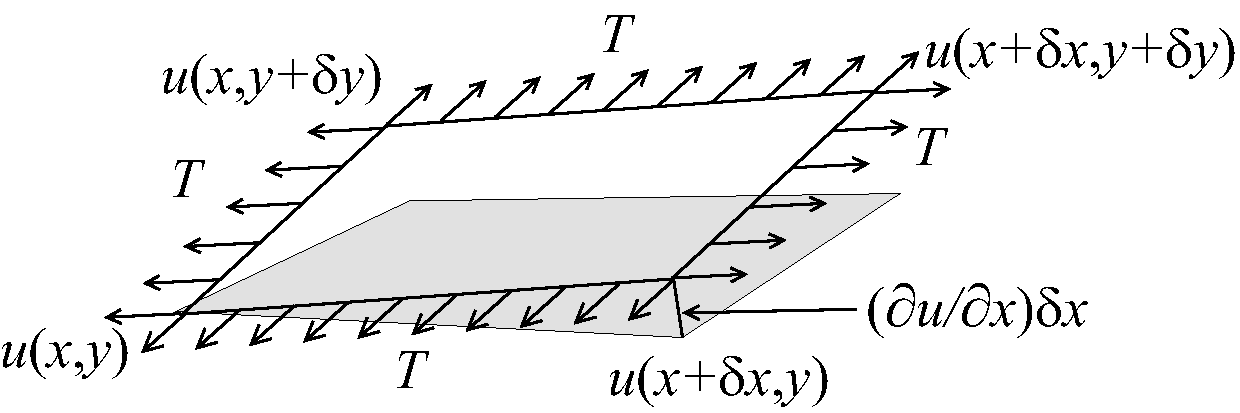
\includegraphics[height=3cm]{soapfilm}
\end{center}
%\caption{``small plane'' ABCD}
\label{fig:soapfilm}
\end{figure}
Similarly, for the edges AB and DC we have
\[
-\mu n_y(x,y)\delta x,\qquad
\mu\left(n_y(x,y)+\p n_y/\p y\right)(x,y)\delta x.
\]
The force in the vertical direction on the surface ABCD due to the tension $\mu$ is given by
\[
\mu\left(\p n_x/\p x\right)\delta x\delta y+T\left(\p n_y/\p y\right)\delta y\delta x.
\]
Assuming small displacements, we have
\begin{eqnarray*}
\nu_x&=&(\p u/\p x)/\sqrt{1+(\p u/\p x)^2+(\p u/\p y)^2}\simeq \p u/\p x,\\
\nu_y&=&(\p u/\p y)/\sqrt{1+(\p u/\p x)^2+(\p u/\p y)^2}\simeq \p u/\p y.
\end{eqnarray*}
Letting $\delta x\to dx,\, \delta y\to dy$, we have the equilibrium of the vertical displacement of soap film on ABCD by $p$
\[
\mu dx dy\p^2 u/\p x^2 +  \mu dx dy\p^2 u/\p y^2
+ p dx dy = 0.
\]
Using the Laplace operator $\Delta = \p^2 /\p x^2 + \p^2 /\p y^2$, we can find the virtual displacement write the following
\begin{equation}
-\Delta u = f\quad \mbox{in }\Omega
\end{equation}%
where $f=p/\mu$, $\Omega =\{(x,y);\;x^{2}+y^{2}<1\}$.
 Poisson's equation (\ref{eqn:Poisson}) appear
also in \textbf{electrostatics} taking the form of $f=\rho /\epsilon $ where
$\rho $ is the charge density, $\epsilon $ the dielectric constant and $u$
is named as electrostatic potential. The soap film is glued to the ring $%
\p \Omega =C$, then we have the boundary condition
\begin{equation}
u=0\quad \mbox{on }\p \Omega
\end{equation}%
If the force is gravity, for simplify, we assume that $f=-1$.


\begin{example}[a\_tutorial.edp]~
\index{tutorial!aTutorial.edp}
\bFF
 1 : @border a(t=0,2*pi){ x = cos(t); y = sin(t);label=1;};
 2 :
 3 : @mesh disk = @buildmesh(a(50));
 4 : @plot(disk);
 5 : @fespace femp1(disk,P1);
 6 : femp1 u,v;
 7 : @func f = -1;
 8 : @problem laplace(u,v) =
 9 :     @int2d(disk)( @dx(u)*@dx(v) + @dy(u)*@dy(v) )     //  bilinear form
10 :   - @int2d(disk)( f*v )                          //  linear form
11 :   + @on(1,u=0) ;                                // boundary condition
12 : @func ue = (x^2+y^2-1)/4;   // ue: exact solution
13 : laplace;
14 : femp1 err = u - ue;
15 :
16 : @plot (u,ps="aTutorial.eps",value=true,wait=true);
17 : @plot(err,value=true,wait=true);
18 :
19 : @cout << "error L2=" << @sqrt(@int2d(disk)( err^2) )<< @endl;
20 : @cout << "error H10=" << @sqrt( @int2d(disk)((dx(u)-x/2)^2)
21 :                               + @int2d(disk)((dy(u)-y/2)^2))<< @endl;
22 :
23 : disk = @adaptmesh(disk,u,err=0.01);
24 : @plot(disk,wait=1);
25 :
26 : laplace;
27 :
28 : @plot (u,value=true,wait=true);
29 : err = u - ue;  // become FE-function on adapted mesh
30 : @plot(err,value=true,wait=true);
31 : cout << "error L2=" << @sqrt(@int2d(disk)( err^2) )<< endl;
32 : cout << "error H10=" << @sqrt(@int2d(disk)((@dx(u)-x/2)^2)
33 :                              + @int2d(disk)((@dy(u)-y/2)^2))<< endl;
\eFF
\end{example}
\begin{figure}[htbp]
\begin{minipage}{\textwidth}
\begin{minipage}{0.4\textwidth}
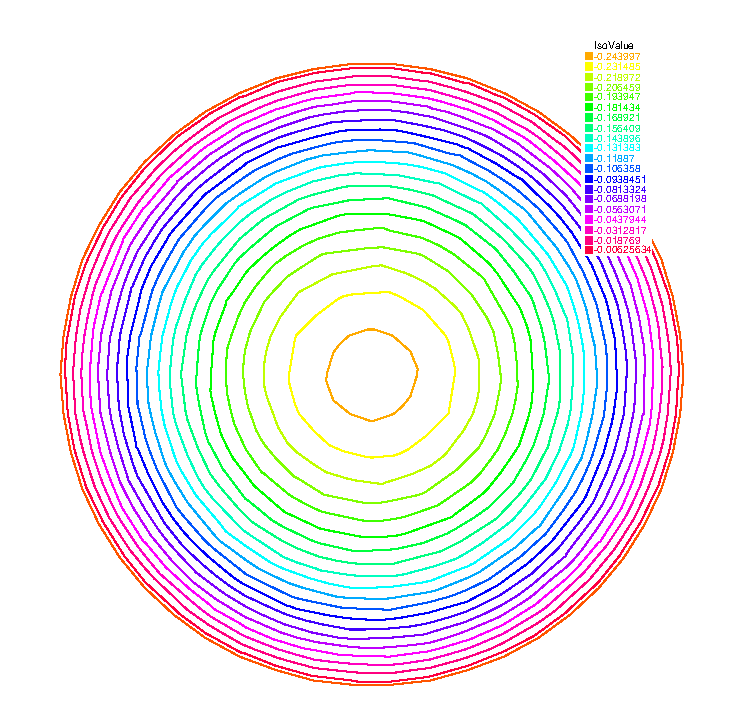
\includegraphics[width=\textwidth]{aTutorial}%
\caption{isovalue of $u$}
\label{aTutorial}
\end{minipage}
\hspace{0.5mm}
\begin{minipage}{0.6\textwidth}
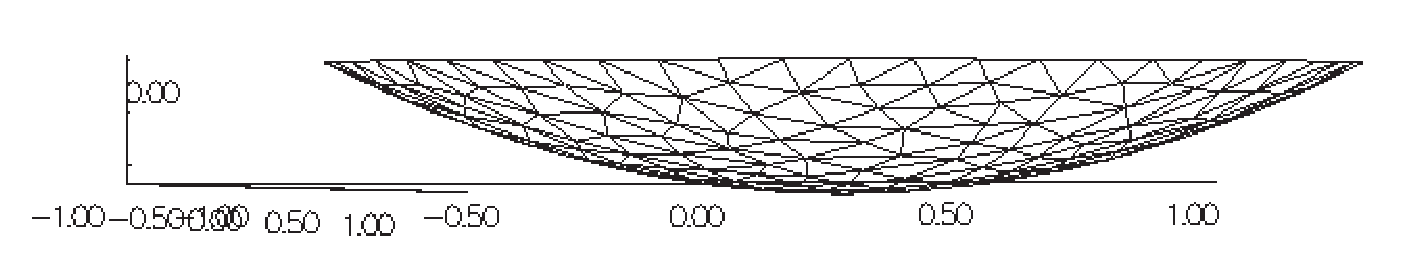
\includegraphics[width=\textwidth]{soapfilm3d}%
\caption{a side view of $u$}
\end{minipage}
\end{minipage}
\end{figure}

In 19th line, the $L^2$-error estimation between the exact solution $u_e$,
$$
\|u_h - u_e\|_{0,\Omega}=\left(\int_{\Omega}|u_h-u_e|^2\, \d x\d y\right)^{1/2}
$$
and from 20th line to 21th line, the $H^1$-error seminorm estimation
$$
|u_h - u_e|_{1,\Omega}=\left(\int_{\Omega}|\nabla u_h-\nabla u_e|^2\, \d x\d y\right)^{1/2}
$$
are done on the initial mesh. The results are
$\|u_h - u_e\|_{0,\Omega}=0.000384045,\, |u_h - u_e|_{1,\Omega}=0.0375506$.

After the adaptation, we hava
$\|u_h - u_e\|_{0,\Omega}=0.000109043,\, |u_h - u_e|_{1,\Omega}=0.0188411$.
So the numerical solution is improved by adaptation of mesh.


\subsubsection{Electrostatics}
We assume that there is no current and a time independent charge distribution.
Then the electric field $\vec E$ satisfy
\begin{eqnarray}
\label{eqn:Maxwell0}
\mathrm{div}\vec E=\rho/\epsilon,\quad \mathrm{curl}\vec E=0
\end{eqnarray}
where $\rho$ is the charge density and $\epsilon$ is called the permittivity of free space. From the second equation in (\ref{eqn:Maxwell0}), we can introduce
the electrostatic potential such that $\vec E=-\nabla \phi$.
Then we have Poisson equation $-\Delta \phi=f$, $f=-\rho/\epsilon$.
We now obtain the equipotential line which is the level curve of $\phi$,
when there are no charges except conductors $\{C_i\}_{1,\cdots,K}$.
Let us assume $K$ conductors $C_1,\cdots,C_K$ within an enclosure $C_0$.
Each one is held
at an electrostatic potential $\varphi_i$. We assume that the enclosure $C0$ is
held at
potential 0.
In order to know $\varphi(x)$ at any point $x$ of the domain $\Omega$, we must
solve
\begin{equation}
-\Delta \varphi =0\quad \textrm{in  }\Omega ,
\end{equation}
where $\Omega$ is the interior of $C_0$ minus the conductors $C_i$, and
$\Gamma$ is the boundary of $\Omega$, that is $\sum_{i=0}^N C_i$.
Here $g$ is any function of $x$ equal to $\varphi_i$ on $C_i$ and to
0 on $C_0$. The second equation is a reduced form for:
\begin{equation}
\varphi =\varphi _{i}\;\text{on }C_{i},\;i=1...N,\varphi =0\;\text{on\ }%
C_{0}.
\end{equation}
\begin{example}~
First we give the geometrical informations; $C_0=\{(x,y);\; x^2+y^2=5^2\}$,
$C_1=\{(x,y):\; \frac{1}{0.3^2}(x-2)^2+\frac{1}{3^2}y^2=1\}$,
$C_2=\{(x,y):\; \frac{1}{0.3^2}(x+2)^2+\frac{1}{3^2}y^2=1\}$.
Let $\Omega$ be the disk enclosed by $C_0$ with the elliptical holes enclosed
by $C_1$ and $C_2$. Note that $C_0$ is described counterclockwise, whereas the
elliptical holes are described clockwise, because the boundary must be oriented so that the computational domain is to its left.
\bFF
// a circle with center at (0 ,0) and radius 5
border C0(t=0,2*pi) { x = 5 * cos(t); y = 5 * sin(t); }
border C1(t=0,2*pi) { x = 2+0.3 * cos(t); y = 3*sin(t); }
border C2(t=0,2*pi) { x = -2+0.3 * cos(t); y = 3*sin(t); }

mesh Th = buildmesh(C0(60)+C1(-50)+C2(-50));
plot(Th,ps="electroMesh"); // figure \ref{electroMesh}
fespace Vh(Th,P1);     // P1 FE-space
Vh uh,vh;              // unknown and test function.
problem Electro(uh,vh) =  //  definition of  the problem
    int2d(Th)( dx(uh)*dx(vh) + dy(uh)*dy(vh) ) //  bilinear
    + on(C0,uh=0)       //  boundary condition on $C_0$
    + on(C1,uh=1)       //  +1 volt on $C_1$
    + on(C2,uh=-1) ;    //  -1 volt on $C_2$

Electro; // solve the problem, see figure \ref{electro} for the solution
plot(uh,ps="electro.eps",wait=true); // figure \ref{electro}
\eFF
\end{example}

\twoplot[height=5cm]{electroMesh}{electro}{Disk with two elliptical holes}
{Equipotential lines, where $C_1$ is located in right hand side}

\subsubsection{Aerodynamics}
Let us consider a wing profile $S$ in a uniform flow.
Infinity will be represented
by a large circle $\Gamma_{\infty}$.
As previously, we must solve
\begin{equation}
\label{eqn:NACA-5-5}
\Delta \varphi=0\quad\textrm{in }\Omega,
\quad \varphi|_S=c,\quad
\varphi|_{\Gamma_{\infty}}=u_{\infty 1x}-u_{\infty2x}
\end{equation}
where $\Omega$ is the area occupied by the
fluid, $u_{\infty}$ is the air speed at infinity, $c$
is a constant to be determined so that
$\p_n\varphi$ is continuous at the trailing edge
$P$ of $S$ (so-called Kutta-Joukowski condition).
Lift is proportional to $c$.
To find $c$ we use a superposition method. As all equations in
(\ref{eqn:NACA-5-5}) are
linear, the solution $\varphi_c$ is a linear function of $c$
\begin{equation}
\label{eqn:NACA-5-6}
\varphi_c = \varphi_0 + c\varphi_1,
\end{equation}
where $\varphi_0$ is a solution of (\ref{eqn:NACA-5-5}) with $c = 0$ and
$\varphi_1$ is a solution with $c = 1$ and
zero speed at infinity.
With these two fields computed, we shall determine $c$
by requiring the continuity of $\p \varphi /\p n$ at the trailing edge.
An equation for the upper surface of a NACA0012 (this is a classical wing
profile in aerodynamics; the rear of the wing is called the trailing edge) is:
\begin{equation}
\label{eqn:NACA-5-7} y = 0.17735\sqrt{x} - 0.075597x - 0.212836x^2 +
0.17363x^3 - 0.06254x^4.
\end{equation}
Taking an incidence angle $\alpha$ such that $\tan \alpha = 0.1$, we must solve
\begin{equation}
\label{eqn:NACA-5-8}
-\Delta\varphi  = 0\qquad \textrm{in }\Omega, \qquad
\varphi|_{\Gamma_1} = y - 0.1x,\quad \varphi |_{\Gamma_2} = c,
\end{equation}
where $\Gamma_2$ is the wing profile and $\Gamma_1$ is an approximation of
infinity. One finds $c$ by solving:
\begin{eqnarray}
\label{eqn:NACA-5-9}
-\Delta\varphi_0 = 0 ~~\textrm{in }\Omega,\qquad
\varphi_0|_{\Gamma_1} = y - 0.1x, \quad \varphi_0|_{\Gamma_2} = 0,\\
\label{eqn:NACA-5-10}
-\Delta\varphi_1 = 0 ~~\textrm{in }\Omega, \qquad
\varphi_1|_{\Gamma_1} = 0, \quad \varphi_1|_{\Gamma_2} = 1.
\end{eqnarray}
The solution $\varphi  = \varphi_0+c\varphi_1$ allows us to find $c$
by writing that $\p_n\varphi$  has no jump
at the trailing edge $P = (1, 0)$.
We have $\p n\varphi  -(\varphi (P^+)-\varphi (P))/\delta$ where $P^+$
is the point just above $P$ in the direction normal to the profile at a distance
$\delta$. Thus the jump of $\p_n\varphi$  is
$(\varphi_0|_{P^+} +c(\varphi_1|_{P^+} -1))+(\varphi_0|_{P^-} +c(\varphi_1|_{P^-} -1))$
divided by $\delta$ because the normal changes sign between the lower and upper
surfaces. Thus
\begin{equation}
\label{eqn:NACA-5-11}
c = -\frac{\varphi_0|_{P^+} + \varphi_0|_{P^-}}
{(\varphi_1|_{P^+} + \varphi_1|_{P^-} - 2)} ,
\end{equation}
which can be programmed as:
\begin{equation}
\label{eqn:NACA-5-12}
c = -\frac{\varphi_0(0.99, 0.01) + \varphi_0(0.99,-0.01)}
{(\varphi_1(0.99, 0.01) + \varphi_1(0.99,-0.01) - 2)} .
\end{equation}

\begin{example}
\bFF

// Computation of the potential flow around a NACA0012 airfoil.
// The method of decomposition is used to apply the Joukowski condition
// The solution is seeked in the form psi0 + beta psi1 and beta is
// adjusted so that the pressure is continuous at the trailing edge

@border a(t=0,2*pi) { x=5*cos(t);  y=5*sin(t); };// approximates infinity

@border upper(t=0,1) { x = t;
     y = 0.17735*sqrt(t)-0.075597*t
  - 0.212836*(t^2)+0.17363*(t^3)-0.06254*(t^4); }
@border lower(t=1,0) { x = t;
     y= -(0.17735*sqrt(t)-0.075597*t
  -0.212836*(t^2)+0.17363*(t^3)-0.06254*(t^4)); }
@border c(t=0,2*pi) { x=0.8*cos(t)+0.5;  y=0.8*sin(t); }

@wait = @true;
@mesh  Zoom = @buildmesh(c(30)+upper(35)+lower(35));
@mesh Th = @buildmesh(a(30)+upper(35)+lower(35));
@fespace Vh(Th,P2);     // P1 FE space
Vh psi0,psi1,vh;              // unknown and test function.
@fespace ZVh(Zoom,P2);

@solve Joukowski0(psi0,vh) =     //  definition of  the problem
    @int2d(Th)( dx(psi0)*dx(vh) + dy(psi0)*dy(vh) ) //  bilinear form
  + @on(a,psi0=y-0.1*x)                      //  boundary condition form
  + @on(upper,lower,psi0=0);
@plot(psi0);

@solve Joukowski1(psi1,vh) =     //  definition of  the problem
    @int2d(Th)( dx(psi1)*dx(vh) + dy(psi1)*dy(vh) ) //  bilinear form
  + @on(a,psi1=0)                      //  boundary condition form
  + @on(upper,lower,psi1=1);

@plot(psi1);

    // continuity of pressure at trailing edge
@real beta = psi0(0.99,0.01)+psi0(0.99,-0.01);
@beta = -beta / (psi1(0.99,0.01)+ psi1(0.99,-0.01)-2);


Vh psi = beta*psi1+psi0;
@plot(psi);
ZVh Zpsi=psi;
@plot(Zpsi,bw=true);
Vh cp = -dx(psi)^2 - dy(psi)^2;
@plot(cp);
ZVh Zcp=cp;
@plot(Zcp,nbiso=40);
\eFF
\end{example}
\twoplot[height=5cm]{naca1}{naca2}
{isovalue of $cp = -(\p_x\psi)^2 - (\p_y\psi)^2$}
{Zooming of $cp$}


\subsubsection{Error estimation}
There are famous estimation between the numerical result $u_h$ and the
exact solution $u$ of the problem \ref{eqn:Poisson} and \ref{eqn:Dirichlet}:
If triangulations $\{\mathcal{T}_h\}_{h\downarrow 0}$ is regular
(see \refSec{Regular Triangulation}), then we have the estimates
\begin{eqnarray}
\label{eqn:H1err}
|\nabla u - \nabla u_h|_{0,\Omega}&\le& C_1h\\
\label{eqn:L2err}
\|u - u_h\|_{0,\Omega}&\le& C_2h^2
\end{eqnarray}
with constants $C_1,\, C_2$ independent of $h$,
if $u$ is in $H^2(\Omega)$. It is known that $u\in H^2(\Omega)$
if $\Omega$ is convex.

In this section we check (\ref{eqn:H1err}) and (\ref{eqn:L2err}).
We will pick up numericall error if we use the numerical derivative,
so we will use the following for (\ref{eqn:H1err}).
\begin{eqnarray*}
\int_{\Omega}|\nabla u - \nabla u_h|^2\, \d x\d y
&=&\int_{\Omega}\nabla u\cdot \nabla(u - 2u_h)\, \d x\d y+
\int_{\Omega}\nabla u_h\cdot \nabla u_h\, \d x\d y\\
&=&\int_{\Omega}f(u-2u_h)\, \d x\d y+\int_{\Omega}fu_h\, \d x\d y
\end{eqnarray*}
The constants $C_1,\, C_2$ are depend on $\mathcal{T}_h$ and $f$,
so we will find them by \freefempp.
In general, we cannot get the solution $u$ as a elementary functions
(see Section \ref{sec:TwoVarFunctions}) even if spetical functions are added.
Instead of the exact solution, here we use the approximate solution $u_0$  in
$V_h(\mathcal{T}_h,P_2),\, h\sim 0$.

\begin{example}~
\bFF
 1 : @mesh Th0 = @square(100,100);
 2 : @fespace V0h(Th0,P2);
 3 : V0h u0,v0;
 4 : @func f = x*y; // sin(pi*x)*cos(pi*y);
 5 :
 6 : @solve Poisson0(u0,v0) =
 7 :     @int2d(Th0)( @dx(u0)*@dx(v0) + @dy(u0)*@dy(v0) )     //  bilinear form
 8 :   - @int2d(Th0)( f*v0 )                          //  linear form
 9 :   + @on(1,2,3,4,u0=0) ;                // boundary condition
10 :
11 : @plot(u0);
12 :
13 : @real[int] errL2(10), errH1(10);
14 :
15 : @for (@int i=1; i<=10; i++) {
16 :    @mesh Th = @square(5+i*3,5+i*3);
17 :    @fespace Vh(Th,P1);
18 :    @fespace Ph(Th,P0);
19 :    Ph h = hTriangle;  // get the size of all triangles
20 :    Vh u,v;
21 :    @solve Poisson(u,v) =
22 :         @int2d(Th)( dx(u)*dx(v) + dy(u)*dy(v) )     //  bilinear form
23 :         - @int2d(Th)( f*v )                          //  linear form
24 :         + @on(1,2,3,4,u=0) ;                // boundary condition
25 :    V0h uu = u;
26 :    errL2[i-1] = @sqrt( @int2d(Th0)((uu - u0)^2) )/h[].max^2;
27 :    errH1[i-1] = @sqrt( @int2d(Th0)( f*(u0-2*uu+uu) ) )/h[].max;
28 : }
29 : @cout << "C1 = " << errL2.max <<"("<<errL2.min<<")"<< endl;
30 : @cout << "C2 = " << errH1.max <<"("<<errH1.min<<")"<< endl;
\eFF
\end{example}
We can guess that $C_1=0.0179253(0.0173266)$ and
$C_2=0.0729566(0.0707543)$, where the numbers inside the parentheses
are minimum in calculation.

\subsubsection{Periodic }\index{periodic}\index{fespace!periodic=}
We now solve the Poisson equation
$$ -\Delta u= sin(x+\pi/4.)*cos(y+\pi/4.)$$ on
the square $]0,2\pi[^2$
under bi-periodic boundary condition
$u(0,y)=u(2\pi,y)$ for all $y$ and
$u(x,0)=u(x,2\pi)$ for all $x$.
These boundary conditions are achieved from the definition
of the periodic finite element space.

\begin{example}[periodic.edp]~
\label{exm:periodic}
\index{tutorial!periodic.edp}
\bFF
@mesh Th=square(10,10,[2*x*pi,2*y*pi]);
// defined the \bgroup\tt fespace\egroup  with periodic condition
//    label :  2 and 4  are left and right   side with y the curve abscissa
//             1 and 2  are bottom and upper side with x the curve abscissa
@fespace Vh(Th,P2,periodic=[[2,y],[4,y],[1,x],[3,x]]);
 Vh uh,vh;              // unknown and test function.
 @func f=sin(x+pi/4.)*cos(y+pi/4.);      //  right hand side function

@ problem laplace(uh,vh) =                      //  definion of  the problem
    @int2d(Th)( dx(uh)*dx(vh) + dy(uh)*dy(vh) ) //  bilinear form
  + @int2d(Th)( -f*vh )                         //  linear form
;

  @laplace; // solve the problem plot(uh); // to see the result
  @plot(uh,ps="period.eps",value=true);
\eFF
\plot[height=6cm]{period}{The isovalue of solution $u$ with periodic boundary condition}
\end{example}

The periodic condition does not necessarily require
parallel to the axis. Example \ref{exm:periodic4}
 give such example.

\begin{example}[periodic4.edp]~
\label{exm:periodic4}
\index{tutorial!periodic4.edp}
\bFF
@real r=0.25;
// a diamond with a hole
@border a(t=0,1){x=-t+1; y=t;label=1;};
@border b(t=0,1){ x=-t; y=1-t;label=2;};
@border c(t=0,1){ x=t-1; y=-t;label=3;};
@border d(t=0,1){ x=t; y=-1+t;label=4;};
@border e(t=0,2*pi){ x=r*cos(t); y=-r*sin(t);label=0;};
@int n = 10;
@mesh Th= buildmesh(a(n)+b(n)+c(n)+d(n)+e(n));
@plot(Th,wait=1);
@real r2=1.732;
@func abs=sqrt(x^2+y^2);
//  warning for periodic condition: \hfilll
//  side a and c \hfilll
//  @on side a (label 1) $ x \in [0,1] $ or $ x-y\in [-1,1] $ \hfilll
//  @on side c (label 3) $ x \in [-1,0]$ or $ x-y\in[-1,1] $\hfilll
// so the common abscissa can be respectively $x$ and $x+1$
// or you can can try curviline abscissa $x-y$ and $x-y$
//  1 first way \hfilll
// @fespace Vh(Th,P2,periodic=[[2,1+x],[4,x],[1,x],[3,1+x]]);  \hfilll
// 2 second way \hfilll
 @fespace Vh(Th,P2,periodic=[[2,x+y],[4,x+y],[1,x-y],[3,x-y]]);

 Vh uh,vh;

 @func f=(y+x+1)*(y+x-1)*(y-x+1)*(y-x-1);
 @real intf = @int2d(Th)(f);
 @real mTh = @int2d(Th)(1);
 @real k =  intf/mTh;
 @cout << k << @endl;
 @problem laplace(uh,vh) =
    @int2d(Th)( dx(uh)*dx(vh) + dy(uh)*dy(vh) ) + @int2d(Th)( (k-f)*vh ) ;
 laplace;
 @plot(uh,wait=1,ps="perio4.eps");
\eFF
\end{example}
\plot[height=6cm]{perio4}{The isovalue of solution $u$ for
$ \Delta u = ((y+x)^{2}+1)((y-x)^{2}+1) - k$, in $\Omega$ and $\p_{n} u =0 $ on hole,and with two periodic boundary condition on external border}


\subsubsection{Poisson with mixed boundary condition}
Here we consider the Poisson equation with mixed boundary value
problems: For given functions $f$ and $g$, find $u$ such that
\begin{eqnarray}
\label{eqn:mixBoundary}
-\Delta u &=& f\qquad \textrm{in }\Omega\nonumber\\
u&=&g\quad \textrm{on }\Gamma_D,\quad
\p u/\p n=0\quad \textrm{on }\Gamma_N
\end{eqnarray}
where $\Gamma_D$ is a part of the boundary $\Gamma$ and
$\Gamma_N=\Gamma\setminus \overline{\Gamma_D}$.
The solution $u$ has the singularity at the points
$\{\gamma_1,\gamma_2\}=\overline{\Gamma_D}\cap\overline{\Gamma_N}$.
When $\Omega=\{(x,y);\; -1<x<1,\, 0<y<1\}$,
$\Gamma_N=\{(x,y);\; -1\le x<0,\, y=0\}$,\,
$\Gamma_D=\p \Omega\setminus \Gamma_N$,
the singularity will appear at $\gamma_1=(0,0),\, \gamma_2(-1,0)$,
and $u$ has the expression
$$
u=K_iu_S + u_R,\, u_R\in H^2(\textrm{near }\gamma_i),\, i=1,2
$$
with a constants $K_i$.
Here $u_S = r_j^{1/2}\sin(\theta_j/2)$ by the local polar coordinate
$(r_j,\theta_j$ at $\gamma_j$ such that
$(r_1,\theta_1)=(r,\theta)$.
Instead of poler coordinate system $(r,\theta)$, we use that
$r=\ttCC{sqrt( x\^2+y\^2 )}$ and $\theta = \ttCC{atan2(y,x)}$
in \freefempp.

\begin{example} Assume that $f=-2\times 30(x^2+y^2)$ and
$g=u_e=10(x^2+y^2)^{1/4}\sin\left ([\tan^{-1}(y/x)]/2\right)
+30(x^2y^2)$, where $u_e$S is the exact solution.
\bFF
 1 : @border N(t=0,1) { x=-1+t; y=0; label=1; };
 2 : @border D1(t=0,1){ x=t;  y=0; label=2;};
 3 : @border D2(t=0,1){ x=1; y=t; label=2; };
 4 : @border D3(t=0,2){ x=1-t; y=1; label=2;};
 5 : @border D4(t=0,1) { x=-1; y=1-t; label=2; };
 6 :
 7 : @mesh T0h = @buildmesh(N(10)+D1(10)+D2(10)+D3(20)+D4(10));
 8 : @plot(T0h,wait=true);
 9 : @fespace V0h(T0h,P1);
10 : V0h u0, v0;
11 :
12 : @func f=-2*30*(x^2+y^2); // given function
13 : // the singular term of the solution is K*us (K: constant)
14 : @func us = sin(atan2(y,x)/2)*sqrt( sqrt(x^2+y^2) );
15 : @real K=10.;
16 : @func ue = K*us + 30*(x^2*y^2);
17 :
18 : @solve Poisson0(u0,v0) =
19 :     @int2d(T0h)( dx(u0)*dx(v0) + dy(u0)*dy(v0) )     //  bilinear form
20 :   - @int2d(T0h)( f*v0 )                          //  linear form
21 :   + @on(2,u0=ue) ;                                // boundary condition
22 :
23 : // adaptation by the singular term
24 : @mesh Th = @adaptmesh(T0h,us);
25 : @for (@int i=0;i< 5;i++)
26 : {
27 :   @mesh Th=@adaptmesh(Th,us);
28 : } ;
29 :
30 : @fespace Vh(Th, P1);
31 : Vh u, v;
32 : @solve Poisson(u,v) =
33 :     @int2d(Th)( dx(u)*dx(v) + dy(u)*dy(v) )     //  bilinear form
34 :   - @int2d(Th)( f*v )                          //  linear form
35 :   + @on(2,u=ue) ;                                // boundary condition
36 :
37 : /* plot the solution */
38 : @plot(Th,ps="adaptDNmix.ps");
39 : @plot(u,wait=true);
40 :
41 : Vh uue = ue;
42 : @real  H1e = @sqrt( @int2d(Th)( dx(uue)^2 + dy(uue)^2 + uue^2 ) );
43 :
44 : /* calculate the H1 Sobolev norm */
45 : Vh err0 = u0 - ue;
46 : Vh  err = u - ue;
47 : Vh  H1err0 = @int2d(Th)( dx(err0)^2+dy(err0)^2+err0^2 );
48 : Vh  H1err = @int2d(Th)( dx(err)^2+dy(err)^2+err^2 );
49 : @cout <<"Relative error in first mesh "<< @int2d(Th)(H1err0)/H1e<<@endl;
50 : @cout <<"Relative error in adaptive mesh "<< @int2d(Th)(H1err)/H1e<@<endl;
\eFF
From 24th line to 28th, adaptation of meshes are done using the
base of singular term.
In 42th line, \ttCC{H1e}=$\|u_e\|_{1,\Omega}$ is calculated.
In last 2 lines, the relative errors are calculated, that is,
\begin{eqnarray*}
\|u^0_h-u_e\|_{1,\Omega}/\ttCC{H1e}&=&0.120421\\
\|u^a_h-u_e\|_{1,\Omega}/\ttCC{H1e}&=&0.0150581
\end{eqnarray*}
where $u^0_h$ is the numerical solution in \ttCC{T0h} and
$u^a_h$ is \ttCC{u} in this program.
\end{example}

\subsubsection{Adaptation with residual error indicator}

We do metric mesh adaption and compute the classical
residual error indicator $\eta_{T}$ on the element $T$ for the Poisson problem.

\begin{example}[adaptindicatorP2.edp]~
\index{tutorial!adaptindicatorP2.edp}
First, we solve the same problem as in a previous example.
\bFF
 1 : @border ba(t=0,1.0){x=t;   y=0;  label=1;}; // see Fig,\ref{L-shape2}
 2 : @border bb(t=0,0.5){x=1;   y=t;  label=2;};
 3 : @border bc(t=0,0.5){x=1-t; y=0.5;label=3;};
 4 : @border bd(t=0.5,1){x=0.5; y=t;  label=4;};
 5 : @border be(t=0.5,1){x=1-t; y=1;  label=5;};
 6 : @border bf(t=0.0,1){x=0;   y=1-t;label=6;};
 7 : @mesh Th = buildmesh (ba(6) + bb(4) + bc(4) +bd(4) + be(4) + bf(6));
 8 : @savemesh(Th,"th.msh");
 9 : @fespace Vh(Th,P2);
10 : @fespace Nh(Th,P0);
11 : Vh u,v;
12 : Nh rho;
13 : real[int] viso(21);
14 : @for (@int i=0;i<viso.n;i++)
15 :   viso[i]=10.^(+(i-16.)/2.);
16 : @real error=0.01;
17 : @func f=(x-y);
18 : @problem Probem1(u,v,solver=CG,eps=1.0e-6) =
19 :     @int2d(Th,qforder=5)( u*v*1.0e-10+  dx(u)*dx(v) + dy(u)*dy(v))
20 :   + @int2d(Th,qforder=5)( -f*v);
21 : /*************
\eFF
\index{jump}\index{intalledges}\index{square}\index{lenEdge}\index{hTriangle}%\index{area}
Now, the local  error indicator $\eta_{T}$ is:
\def\Th{\mathcal{T}_{h}}
\def\AK{\mathcal{E}_{K}}

$$\eta_{T} =\left(  h_{T}^{2} || f + \Delta u_{{h}} ||_{L^{2}(T)}^{2} +\sum_{e\in \AK} h_{e} \,||\, [ \frac{\p u_{h}}{\p n_{k}}] \,||^{2}_{L^{2}(e)} \right)^{\frac{1}{2}}
   $$
where $h_{T}$ is the longest's edge of  $T$, ${\cal E}_T$ is the set of $T$ edge not on
$\Gamma=\p \Omega$, $n_{T}$ is the  outside unit normal to $K$, $h_{e}$ is the length of edge $e$,
$[ g ]$ is the jump of the function $g$ across edge (left value minus right value).

Of coarse, we can use a variational form to compute $\eta_{T}^{2}$,
with test function constant function in each triangle.
\bFF
29 : *************/
30 :
31 : @varf indicator2(uu,chiK) =
32 :      @intalledges(Th)(chiK*lenEdge*square(jump(N.x*dx(u)+N.y*dy(u))))
33 :     +@int2d(Th)(chiK*square(hTriangle*(f+dxx(u)+dyy(u))) );
34 : for (int i=0;i< 4;i++)
35 : {
36 :   Probem1;
37 :    @cout << u[].min << " " << u[].max << endl;
38 :    @plot(u,wait=1);
39 :    @cout << " indicator2 " << endl;
40 :
41 :    rho[] = indicator2(0,Nh);
42 :    rho=sqrt(rho);
43 :    @cout << "rho =   min " << rho[].min << " max=" << rho[].max << @endl;
44 :    @plot(rho,fill=1,wait=1,cmm="indicator density ",ps="rhoP2.eps",
                                       value=1,viso=viso,nbiso=viso.n);
45 :    @plot(Th,wait=1,cmm="Mesh ",ps="ThrhoP2.eps");
46 :    Th=@adaptmesh(Th,[dx(u),dy(u)],err=error,anisomax=1);
47 :    @plot(Th,wait=1);
48 :    u=u;
49 :    rho=rho;
50 :   error = error/2;
51 : } ;
\eFF
If the method is correct, we expect to look the graphics by an almost constant function $\eta$ on your computer as in Fig. \ref{fig:rhoP2}.
\begin{figure}[hbt]
\begin{center}
\label{fig:rhoP2}
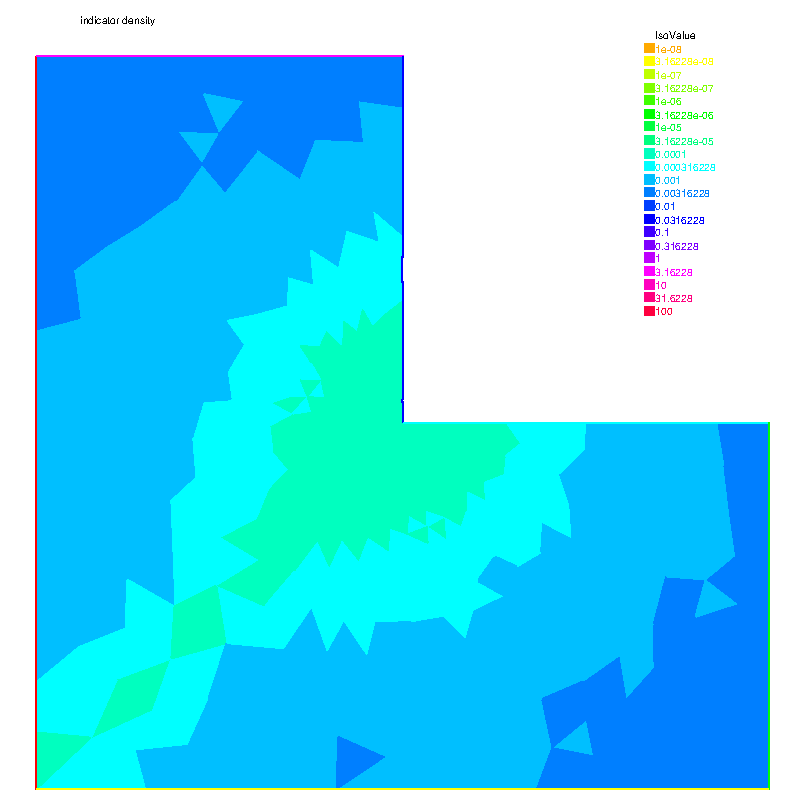
\includegraphics[height=8cm]{rhoP2} 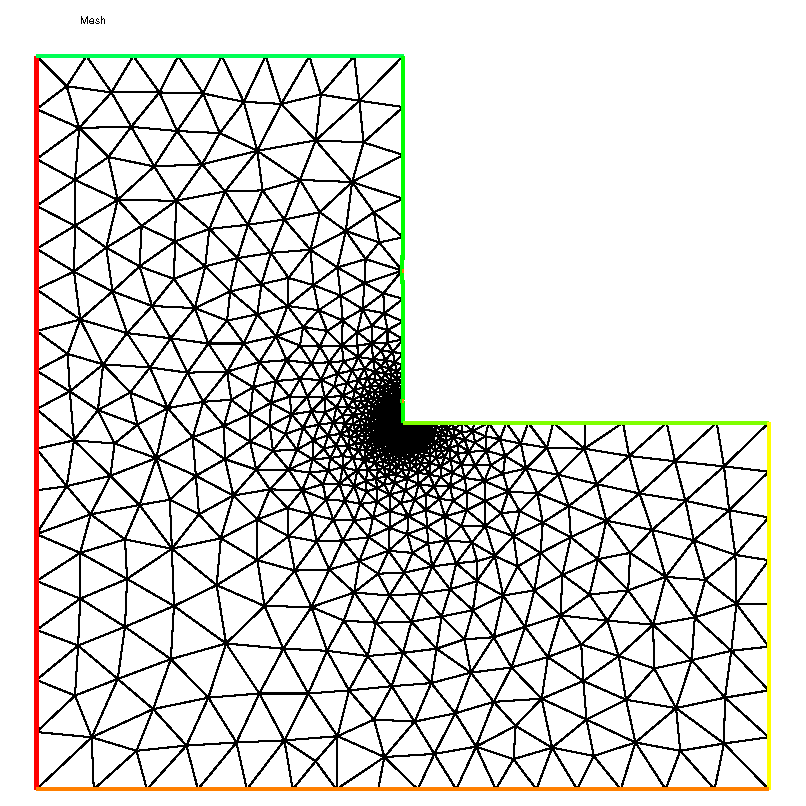
\includegraphics[height=8cm]{ThrhoP2}
\end{center}
\caption{Density of the error indicator  with isotropic $P^{2}$ metric }
\end{figure}
\end{example}


\subsection{Elasticity}

Consider an elastic plate with undeformed shape $\Omega\times ]-h,h[$
in $\R^3$, $\Omega\subset\R^2$.
By the deformation of the plate,
we assume that a point $P(x_1,x_2,x_3)$ moves to
${\cal P}(\xi_1,\xi_2,\xi_3)$.
The vector $\vec u=(u_1,u_2,u_3)=(\xi_1-x_1,\xi_2-x_2,\xi_3-x_3)$ is called
\key{displacement vector}.
By the deformation,
the line segment
$\overline{\mathbf{x},\mathbf{x}+\tau\Delta\mathbf{x}}$ moves approximately to
$\overline{\mathbf{x}+u(\mathbf{x}),\mathbf{x}+\tau\Delta\mathbf{x}
+u(\mathbf{x}+\tau\Delta\mathbf{x})}$ for small $\tau$,
where
$\mathbf{x}=(x_1,x_2,x_3),\, \Delta\mathbf{x}
=(\Delta x_1,\Delta x_2,\Delta x_3)$.
We now calculate the ratio between two segments
\[
\eta(\tau)=\tau^{-1}|\Delta\mathbf{x}|^{-1}
\left(|u(\mathbf{x}+\tau\Delta\mathbf{x})
-u(\mathbf{x})+\tau\Delta\mathbf{x}|-\tau|\Delta\mathbf{x}|\right)
\]
then we have (see e.g. \cite[p.32]{Necas})
\begin{eqnarray*}
\lim_{\tau\to 0}\eta(\tau)=(1+2e_{ij}\nu_i\nu_j)^{1/2}-1,
\quad 2e_{ij}=\frac{\p u_k}{\p x_i}\frac{\p u_k}{\p x_j}+\left(\frac{\p u_i}{\p x_j}+
\frac{\p u_j}{\p x_i}\right)
\end{eqnarray*}
where $\nu_i=\Delta x_i|\Delta\mathbf{x}|^{-1}$. If the deformation is
\emph{small}, then we may consider that
\[
(\p u_k/\p x_i)(\p u_k/\p x_i)\approx 0
\]
and the following is called \emph{small \key{strain tensor}}
\[
\varepsilon_{ij}(u)=\frac{1}{2}\left(\frac{\p u_i}{\p x_j}+
\frac{\p u_j}{\p x_i}\right)
\]
The tensor $e_{ij}$ is called \emph{finite strain tensor}.

Consider the small plane $\Delta \Pi(\mathbf{x})$
centered at $\mathbf{x}$ with the
unit normal direction $\vec n=(n_1,n_2,n_3)$, then the surface
on $\Delta \Pi(\mathbf{x})$ at $\mathbf{x}$ is
\[
(\sigma_{1j}(\mathbf{x})n_j, \sigma_{2j}(\mathbf{x})n_j, \sigma_{3j}(\mathbf{x})n_j)
\]
where $\sigma_{ij}(\mathbf{x})$ is called \key{stress tensor} at $\mathbf{x}$.
Hooke's law is the assumption of a linear relation between $\sigma_{ij}$
and $\varepsilon_{ij}$ such as
\[
\sigma_{ij}(\mathbf{x})=c_{ijkl}(\mathbf{x})\varepsilon_{ij}(\mathbf{x})
\]
with the symmetry $c_{ijkl}=c_{jikl}, c_{ijkl}=c_{ijlk}, c_{ijkl}=c_{klij}$.

If Hooke's tensor $c_{ijkl}(\mathbf{x})$ do not depend on the choice of
coordinate system, the material is called \key{isotropic} at $\mathbf{x}$.
If $c_{ijkl}$ is constant, the material is called \emph{homogeneous}.
In homogeneous isotropic case, there is \emph{Lam\'{e} constants}
$\lambda, \mu$ (see e.g. \cite[p.43]{Necas}) satisfying
\begin{eqnarray}
\label{eqn:isotropic}
\sigma_{ij}=\lambda\delta_{ij}\textrm{div}u+2\mu \varepsilon_{ij}
\end{eqnarray}
where $\delta_{ij}$ is Kronecker's delta.
We assume that
the elastic plate is fixed
on $\Gamma_D\times ]-h,h[,\, \Gamma_D\subset \p\Omega$.
If the body force $f=(f_1,f_2,f_3)$ is given in $\Omega\times]-h,h[$
and surface force $g$ is given in $\Gamma_N\times]-h,h[,
\Gamma_N=\p\Omega\setminus\overline{\Gamma_D}$,
then the equation of equilibrium is given as follows:
\begin{eqnarray}
\label{eqn:elasticity}
-\p_j \sigma_{ij}&=&f_i~~\textrm{in }\Omega\times ]-h,h[,\quad
i=1,2,3\\
\sigma_{ij}n_j&=&g_i~~\textrm{on }\Gamma_N\times ]-h,h[,\quad
u_i=0~~\textrm{on }\Gamma_D\times ]-h,h[,\quad i=1,2,3
\end{eqnarray}

We now explain the plain elasticity.
\begin{description}
\item[Plain strain:]
On the end of plate, the contact condition $u_3=0,\, g_3=$ is satisfied.
In this case, we can suppose that $f_3=g_3=u_3=0$ and
$\vec u(x_1,x_2,x_3)=\overline{u}(x_1,x_2)$ for all $-h<x_3<h$.
\item[Plain stress:]
The cylinder is assumed to be very thin and subjected to no load on the
ends $x_3=\pm h$, that is,
\[
\sigma_{3i}=0,\quad x_3=\pm h,\quad i~1,2,3
\]
The assumption leads that $\sigma_{3i}=0$ in $\Omega\times ]-h,h[$
and $\vec u(x_1,x_2,x_3)=\overline{u}(x_1,x_2)$ for all $-h<x_3<h$.
\item[Generalized plain stress:]
The cylinder is subjected to no load on the ends $x_3=\pm h$.
Introducing the mean values with respect to thickness,
\[
\overline{u}_i(x_1,x_2)=\frac{1}{2h}
\int_{-h}^h u(x_1,x_2,x_3)dx_3
\]
and we derive $\overline{u}_3\equiv 0$. Similarly we define the mean
values $\overline{f},\overline{g}$ of the body force and surface force
as well as the mean values $\overline{\varepsilon}_{ij}$ and
$\overline{\sigma}_{ij}$ of the components of stress and strain, respectively.
\end{description}
In what follows we omit the overlines of
$\overline{u}, \overline{f},\overline{g}, \overline{\varepsilon}_{ij}$ and
$\overline{\varepsilon}_{ij}$.
Then we obtain similar equation of equilibrium given in (\ref{eqn:elasticity})
replacing $\Omega\times ]-h,h[$ with $\Omega$ and changing $i=1,2$.
In the case of plane stress,
$\sigma_{ij}=\lambda^* \delta_{ij}\textrm{div}u+2\mu\varepsilon_{ij},
\lambda^*=(2\lambda \mu)/(\lambda+\mu)$.

The equations of elasticity are naturally written in variational form
for the displacement vector $u(x)\in V$ as
\Blue{$$
\int_\Omega [2\mu\epsilon_{ij}(\vec u)\epsilon_{ij}(\vec v)
+\lambda \epsilon_{ii}(\vec{u})\epsilon_{jj}(\vec v)]
=\int_\Omega \vec f\cdot \vec v +\int_\Gamma \vec g\cdot \vec v,%\`{u}
\forall \vec v\in V
$$}
where $V$ is the linear closed subspace of $H^1(\Omega)^2$.

\begin{example}[Beam.edp]
\index{tutorial!beam.edp}
Consider  elastic plate with the undeformed rectangle shape
$[0,10]\times [0,2]$.
The body force is the gravity force $\vec f$ and the
boundary force $\vec g$ is zero on lower and upper side.
On the two vertical sides of the beam are fixed.
\bFF
//   a weighting beam sitting on a

int bottombeam = 2;
@border a(t=2,0)  { x=0; y=t ;label=1;};        //  left beam
@border b(t=0,10) { x=t; y=0 ;label=bottombeam;};        //  bottom of beam
@border c(t=0,2)  { x=10; y=t ;label=1;};       //  rigth beam
@border d(t=0,10) { x=10-t; y=2; label=3;};     //  top beam
@real E = 21.5;
@real sigma = 0.29;
@real mu = E/(2*(1+sigma));
@real lambda = E*sigma/((1+sigma)*(1-2*sigma));
@real gravity = -0.05;
@mesh th = buildmesh( b(20)+c(5)+d(20)+a(5));
@fespace Vh(th,[P1,P1]);
Vh [uu,vv], [w,s];
@cout << "lambda,mu,gravity ="<<lambda<< " " << mu << " " << gravity << endl;
// deformation of a beam under its own weight
@solve  bb([uu,vv],[w,s])  =
    @int2d(th)(
          2*mu*(dx(uu)*dx(w)+dy(vv)*dy(s)+ ((dx(vv)+dy(uu))*(dx(s)+dy(w)))/2 )
          + lambda*(dx(uu)+dy(vv))*(dx(w)+dy(s))
    )
  + @int2d(th) (-gravity*s)
  + @on(1,uu=0,vv=0)
 ;

@plot([uu,vv],wait=1);
@plot([uu,vv],wait=1,bb=[[-0.5,2.5],[2.5,-0.5]]);
@mesh th1 = movemesh(th, [x+uu, y+vv]);
@plot(th1,wait=1);
\eFF
\end{example}

\subsubsection{Fracture Mechanics}
Consider the plate with the crack whose undeformed shape is
a curve $\Sigma$ with the two edges $\gamma_1,\, \gamma_2$.
We assume the stress tensor $\sigma_{ij}$ is the state of
plate stress regarding $(x,y)\in \Omega_{\Sigma}=\Omega\setminus \Sigma$.
Here $\Omega$ stands for the undeformed shape of elastic plate
without crack.
If the part $\Gamma_N$ of the boundary $\p\Omega$ is fixed
and a load ${\cal L}=(\vec f,\vec g)\in
L^2(\Omega)^2\times L^2(\Gamma_N)^2$  is given,
then the displacement $\vec u$ is the minimizer of the potential energy
functional
\[
{\cal E}(\vec v;{\cal L},\Omega_{\Sigma})
=\int_{\Omega_{\Sigma}}
\{w(x,\vec v)-\vec f\cdot \vec v\}
-\int_{\Gamma_N}\vec g\cdot \vec v\
\]
over the functional space $V(\Omega_{\Sigma})$,
\[
V(\Omega_{\Sigma})
=\left\{ \vec v\in H^1(\Omega_{\Sigma})^2;\;
\vec v=0\quad \hbox{\rm on }
\Gamma_D=\p\Omega\setminus\overline{\Gamma_N}\right\},
\]
where $w(x,\vec v)=\sigma_{ij}(\vec v)\varepsilon_{ij}(\vec v)/2$,
\[
\sigma_{ij}(\vec v)=C_{ijkl}(x)\varepsilon_{kl}(\vec v),\quad
\varepsilon_{ij}(\vec v)=(\p v_i/\p x_j+
\p v_j/\p x_i)/2,
\qquad (C_{ijkl}:\quad \hbox{\rm Hooke's tensor}).
\]
If the elasticity is homogeneous isotropic, then the
displacement $\vec u(x)$ is decomposed in an open neighborhood $U_k$
of $\gamma_k$ as in (see e.g. \cite{Ohtsuka})
\begin{equation}
\label{eqn:SIF}
\vec u(x) =
\sum_{l=1}^2 K_l(\gamma_k) r_k^{1/2} S^C_{kl}(\theta_k)
+ \vec u_{k,R}(x)
\quad \mbox{for }x\in \Omega_{\Sigma}\cap U_k,\, k=1,2
\end{equation}
with $\vec u_{k,R} \in H^2(\Omega_\Sigma\cap U_k)^2$, where
$U_k,\, k=1,2$ are open neighborhoods of $\gamma_k$ such that
$\p L_1\cap U_1=\gamma_1,\, \p L_m\cap U_2=\gamma_2$,
and
\begin{eqnarray}
\label{eqn:SIF2}
 S^C_{k1}(\theta_k) & = & \frac 1 {4\mu} \frac 1 {(2\pi)^{1/2}}
    \left[ \begin{array}{c}
    [2\kappa-1]\cos(\theta_k/2)-\cos(3\theta_k/2)\\
    -[2\kappa+1]\sin(\theta_k/2)+\sin(3\theta_k/2)
    \end{array}\right],\\
 S^C_{k2}(\theta_k) & = & \frac 1 {4\mu} \frac 1 {(2\pi)^{1/2}}
    \left[ \begin{array}{c}
    -[2\kappa-1]\sin(\theta_k/2)+3\sin(3\theta_k/2)\\
    -[2\kappa+1]\cos(\theta_k/2)+\cos(3\theta_k/2)
    \end{array}\right]. \nonumber
\end{eqnarray}
where $\mu$ is the shear modulus of elasticity,
$\kappa=3-4\nu$ ($\nu$ is the Poisson's ratio) for
plane strain and $\kappa=\frac {3-\nu} {1+\nu}$ for plane stress.

The coefficients $K_1(\gamma_i)$ and $K_2(\gamma_i),$ which are important parameters in fracture mechanics,
are called stress intensity factors of the opening mode (mode I)
and the sliding mode (mode II), respectively.

For simplicity, we consider the following simple crack
\[
\Omega=\{(x,y):\; -1<x<1, -1<y<1\},\qquad
\Sigma=\{(x,y):\; -1\le x\le 0, y=0\}
\]
with only one crack tip $\gamma=(0,0)$.
Unfortunately, \freefempp cannot treat crack, so we use the modification
of the domain with U-shape channel (see Fig. \ref{U-shape})
with $d=0.0001$. The undeformed crack $\Sigma$ is approximated by
\begin{eqnarray*}
\Sigma_d&=&\{(x,y):\; -1\le x\le -10*d, -d\le y\le d\}\\
&&\cup\{(x,y):\; -10*d\le x\le 0, -d+0.1*x\le y\le d-0.1*x\}
\end{eqnarray*}
and $\Gamma_D=\ttCC{R}$ in Fig. \ref{U-shape}.
In this example, we use three technique:
\begin{itemize}
\item
Fast Finite Element Interpolator from the mesh \ttCC{Th}
to \ttCC{Zoom} for the scale-up of
near $\gamma$.
\item
After obtaining the displacement vector $\vec u=(u,v)$, we shall watch
the deformation of the crack near $\gamma$ as follows,
\bFF
mesh Plate = movemesh(Zoom,[x+u,y+v]);
plot(Plate);
\eFF
\item
Important technique is adaptive mesh, because the large singularity occur at
$\gamma$
as shown in (\ref{eqn:SIF}).
\end{itemize}
First example create mode I deformation by the opposed surface force
on \ttCC{B} and \ttCC{T}
in the vertical direction of $\Sigma$, and
the displacement is fixed on \ttCC{R}.

In a laboratory, fracture engineer use
photoelasticity to make stress field visible, which
shows the principal stress difference
\begin{eqnarray}
\sigma_1-\sigma_2=\sqrt{(\sigma_{11}-\sigma_{22})^2+4\sigma_{12}^2}
\end{eqnarray}
where $\sigma_1$ and $\sigma_2$ are the principal stresses.
In opening mode, the photoelasticity make symmetric pattern concentrated at
$\gamma$.
\begin{example}[Crack Opening, $K_2(\gamma)=0$]
\bFF{CrackOpen.edp}
@real d = 0.0001;
@int n = 5;
@real cb=1, ca=1, tip=0.0;
@border L1(t=0,ca-d) { x=-cb; y=-d-t; }
@border L2(t=0,ca-d) { x=-cb; y=ca-t; }
@border B(t=0,2) { x=cb*(t-1); y=-ca; }
@border C1(t=0,1) { x=-ca*(1-t)+(tip-10*d)*t; y=d; }
@border C21(t=0,1) { x=(tip-10*d)*(1-t)+tip*t; y=d*(1-t); }
@border C22(t=0,1) { x=(tip-10*d)*t+tip*(1-t); y=-d*t; }
@border C3(t=0,1) { x=(tip-10*d)*(1-t)-ca*t; y=-d; }
@border C4(t=0,2*d) { x=-ca; y=-d+t; }
@border R(t=0,2) { x=cb; y=cb*(t-1); }
@border T(t=0,2) { x=cb*(1-t); y=ca; }
@mesh Th = @buildmesh (L1(n/2)+L2(n/2)+B(n)
                       +C1(n)+C21(3)+C22(3)+C3(n)+R(n)+T(n));
cb=0.1; ca=0.1;
@plot(Th,@wait=1);
@mesh Zoom = @buildmesh (L1(n/2)+L2(n/2)+B(n)+C1(n)
                         +C21(3)+C22(3)+C3(n)+R(n)+T(n));
@plot(Zoom,@wait=1);
@real E = 21.5;
@real sigma = 0.29;
@real mu = E/(2*(1+sigma));
@real lambda = E*sigma/((1+sigma)*(1-2*sigma));
@fespace Vh(Th,[P2,P2]);
@fespace zVh(Zoom,P2);
Vh [u,v], [w,s];
@solve  Problem([u,v],[w,s])  =
    @int2d(Th)(
             2*mu*(dx(u)*dx(w)+ ((dx(v)+dy(u))*(dx(s)+dy(w)))/4 )
             + lambda*(dx(u)+dy(v))*(dx(w)+dy(s))/2
             )
    -@int1d(Th,T)(0.1*(4-x)*s)+@int1d(Th,B)(0.1*(4-x)*s)
    +@on(R,u=0)+on(R,v=0);                // fixed
;

zVh Sx, Sy, Sxy, N;
@for (@int i=1; i<=5; i++)
{
  @mesh Plate = @movemesh(Zoom,[x+u,y+v]); // deformation near $\gamma$
  Sx = lambda*(dx(u)+dy(v)) + 2*mu*dx(u);
  Sy = lambda*(dx(u)+dy(v)) + 2*mu*dy(v);
  Sxy = mu*(dy(u) + dx(v));
  N = 0.1*1*sqrt((Sx-Sy)^2+4*Sxy^2); //principal stress difference
  @if (i==1) {
     @plot(Plate,ps="1stCOD.eps",bw=1); // Fig. \ref{1stMode1}
     @plot(N,ps="1stPhoto.eps",bw=1);   // Fig. \ref{1stMode1}
  } @else @if (i==5) {
     @plot(Plate,ps="LastCOD.eps",bw=1); // Fig. \ref{LastMode1}
     @plot(N,ps="LastPhoto.eps",bw=1);   // Fig. \ref{LastMode1}
     @break;
  }
  Th=@adaptmesh(Th,[u,v]);
  Problem;
}
\eFF
\end{example}

\begin{figure}[hbt]
\begin{multicols}{2}
\begin{center}
\includegraphics*[height=3cm]{1stCOD}\includegraphics*[height=3cm]{1stPhoto}
    \caption{\label{1stMode1} Crack open displacement (COD) and Principal stress difference in the first mesh}
\end{center}
\begin{center}
\includegraphics*[height=3cm]{LastCOD}\includegraphics*[height=3cm]{LastPhoto}
    \caption{\label{LastMode1} COD and Principal stress difference in the last adaptive mesh}
\end{center}
\end{multicols}
\end{figure}
It is difficult to create mode II deformation by the opposed shear force
on \ttCC{B} and \ttCC{T} that is observed in a laboratory.
So we use the body shear force along $\Sigma$, that is, the $x$-component $f_1$
of the body force $\vec f$ is given by
\[
f_1(x,y)=H(y-0.001)*H(0.1-y)-H(-y-0.001)*H(y+0.1)
\]
where $H(t)=1$ if $t>0$; $= 0$ if $t<0$.

\begin{example}[Crack Sliding, $K_2(\gamma)=0$]
\bFF
(use the same mesh Th)
cb=0.01; ca=0.01;
@mesh Zoom = @buildmesh (L1(n/2)+L2(n/2)+B(n)+C1(n)
                         +C21(3)+C22(3)+C3(n)+R(n)+T(n));
(use same FE-space Vh and elastic modulus)
@fespace Vh1(Th,P1);
Vh1 fx = ((y>0.001)*(y<0.1))-((y<-0.001)*(y>-0.1)) ;

@solve  Problem([u,v],[w,s])  =
    @int2d(Th)(
             2*mu*(dx(u)*dx(w)+ ((dx(v)+dy(u))*(dx(s)+dy(w)))/4 )
             + lambda*(dx(u)+dy(v))*(dx(w)+dy(s))/2
             )
    -@int2d(Th)(fx*w)
    +@on(R,u=0)+@on(R,v=0);        // fixed
;

@for (@int i=1; i<=3; i++)
{
  @mesh Plate = @movemesh(Zoom,[x+u,y+v]); // deformation near $\gamma$
  Sx = lambda*(dx(u)+dy(v)) + 2*mu*dx(u);
  Sy = lambda*(dx(u)+dy(v)) + 2*mu*dy(v);
  Sxy = mu*(dy(u) + dx(v));
  N = 0.1*1*sqrt((Sx-Sy)^2+4*Sxy^2); //principal stress difference
  @if (i==1) {
     @plot(Plate,ps="1stCOD2.eps",bw=1); // Fig. \ref{LastMode2}
     @plot(N,ps="1stPhoto2.eps",bw=1);   // Fig. \ref{1stMode2}
  } else if (i==3) {
     @plot(Plate,ps="LastCOD2.eps",bw=1); // Fig. \ref{LastMode2}
     @plot(N,ps="LastPhoto2.eps",bw=1);   // Fig. \ref{LastMode2}
     break;
  }
  Th=@adaptmesh(Th,[u,v]);
  Problem;
}
\eFF
\end{example}
\begin{figure}[hbt]
\begin{multicols}{2}
\begin{center}
\includegraphics*[height=3cm]{1stCOD2}\includegraphics*[height=3cm]{1stPhoto2}
    \caption{\label{1stMode2} (COD) and Principal stress difference in the first mesh}
\end{center}
\begin{center}
\includegraphics*[height=3cm]{LastCOD2}\includegraphics*[height=3cm]{LastPhoto2}
    \caption{\label{LastMode2} COD and Principal stress difference in the last adaptive mesh}
\end{center}
\end{multicols}
\end{figure}


\subsection{Nonlinear Static Problems}
We propose how to solve the following non-linear academic  problem of minimization
of a functional $$J(u) = \int_\Omega f(|\nabla u|^2) - u*b $$
where $u$ is function of $H^1_0(\Omega)$
and $f$ defined by
$$
f(x) = a*x + x-ln(1+x), \quad f'(x) = a+\frac{x}{1+x}, \quad f''(x) =  \frac{1}{(1+x)^2}
$$

\subsubsection{Newton Ralphson algorithm}


Now, we solve the Euler problem $ \nabla J (u) = 0$
with Newton Ralphson algorithm, that is,
$$
u^{n+1} = u^n - ( \nabla^2 J (u^{n}))^{-1}*dJ(u^n)
$$

\index{Newton}
First we introduice the two variational form \texttt{vdJ} and \texttt{vhJ} to
compute respectively $ \nabla J$ and $ \nabla^2 J$
\bFF
//   method of  Newton Ralphson to solve dJ(u)=0; \hfilll
//    $$ u^{n+1} = u^n - (\frac{\p dJ}{\p u_i})^{-1}*dJ(u^n) $$ \hfilll
//   --------------------------------------------- \hfilll
  Ph dalpha ; //to store = $f''( |\nabla u|^2) $  optimisation


  // the variational form of evaluate  dJ = $ \nabla J$ \hfilll
  // -------------------------------------- \hfilll
  //  dJ =  f'()*( dx(u)*dx(vh) + dy(u)*dy(vh) \hfilll
  @varf vdJ(uh,vh) =  int2d(Th)( alpha*( dx(u)*dx(vh) + dy(u)*dy(vh) ) - b*vh)
  + on(1,2,3,4, uh=0);


  // the variational form of evaluate  ddJ   $= \nabla^2 J$ \hfilll
  // hJ(uh,vh) =  f'()*( dx(uh)*dx(vh) + dy(uh)*dy(vh) \hfilll
  //            + f''()( dx(u)*dx(uh) + dy(u)*dy(uh) ) * (dx(u)*dx(vh) + dy(u)*dy(vh)) \hfilll
  @varf vhJ(uh,vh) = int2d(Th)( alpha*( dx(uh)*dx(vh) + dy(uh)*dy(vh) )
   +  dalpha*( dx(u)*dx(vh) + dy(u)*dy(vh)  )*( dx(u)*dx(uh) + dy(u)*dy(uh) ) )
   + on(1,2,3,4, uh=0);

 // the Newton algorithm \hfilll
  Vh v,w;
  u=0;
  @for (int i=0;i<100;i++)
   {
    alpha = df( dx(u)*dx(u) + dy(u)*dy(u) ) ; // optimization
    dalpha = ddf( dx(u)*dx(u) + dy(u)*dy(u) ) ; // optimization
    v[]= vdJ(0,Vh);  // $ v = \nabla J(u) $
    real res= v[]'*v[]; // the dot product
    cout << i <<  " residu^2 = " <<  res  << endl;
    @if( res< 1e-12) @break;
    @matrix H= vhJ(Vh,Vh,factorize=1,solver=LU); //\index{matrix!factorize=}
    w[]=H^-1*v[];
    u[] -= w[];
   }
   plot (u,wait=1,cmm="solution with Newton Ralphson");
\eFF

\subsection{Eigenvalue Problems}

This section depend on your FreeFem++ compilation process (see \texttt{README\_arpack}),
of this tools.
This tools is available in \texttt{FreeFem++}  if the word ``eigenvalue'' appear in line ``Load:'', like:
\bFF
-- FreeFem++ v1.28 (date Thu Dec 26 10:56:34 CET 2002)
 file : LapEigenValue.edp
 Load: lg_fem lg_mesh @eigenvalue
\eFF
This tools is based on the \texttt{arpack++} \footnote{\url{http://www.caam.rice.edu/software/ARPACK/}}
the object-oriented version of ARPACK eigenvalue package \cite{arpack}.

The function EigenValue compute the generalized eigenvalue
of  $ A u = \lambda B u $ where sigma =$\sigma$ is the shift of the method.
The matrix  $ OP$ is defined with $ A - \sigma B $.
The return value is the number of converged eigenvalue (can be greater than the number of eigen value nev=)

\bFF
@int k=@EigenValue(OP,B,nev= , sigma= );
\eFF
where the matrix $OP=  A - \sigma B $ with a solver and boundary condition,
and the matrix $B$.

\begin{description}
          \item[\texttt{sym=}]    the problem is symmetric (all the eigen value are real)
          \item[\texttt{nev=}]    the number desired eigenvalues (nev)  close to the shift.
        \item[\texttt{value=}]    the array to store the real part of the eigenvalues
         \item[\texttt{ivalue=}]     the array to store the imag. part of the eigenvalues
         \item[\texttt{vector=}]    the array to store the eigenvectors.
 For real nonsymmetric problems, complex eigenvectors are given as two consecutive vectors, so if eigenvalue $k$ and $k+1$ are complex conjugate eigenvalues, the $k$th vector will contain the real part and the $k+1$th vector the imaginary part of the corresponding complex conjugate eigenvectors.

         \item[\texttt{tol=}]        the relative accuracy to which eigenvalues are to be determined;
         \item[\texttt{sigma=}]    the shift value;
         \item[\texttt{maxit=}]    the maximum number of iterations allowed;
          \item[\texttt{ncv=}]     the number of Arnoldi vectors generated at each iteration of ARPACK.
 \end{description}


\begin{example}[lapEignenValue.edp]
\label{exm:lapEigenValue}
In the first example, we compute   the eigenvalue and the eigenvector of the
 Dirichlet problem  on square $\Omega=]0,\pi[^2$.

The problem is find:   $\lambda$, and $\nabla u_{\lambda}$  in $\mathbb{R}{\times} H^1_0(\Omega)$
$$ \int_\Omega \nabla u_{\lambda} \nabla v = \lambda \int_\Omega u  v \quad  \forall v \in H^1_0(\Omega)$$

The exact
eigenvalues are $\lambda_{n,m} =(n^2+m^2), (n,m)\in {\mathbb{N}_*}^2$ with
the associated eigenvectors are  $  u_{{m,n}}=sin(nx)*sin(my)$.



We use the generalized inverse shift mode of the \texttt{arpack++} library, to find
20 eigenvalue and eigenvector close to the shift value $\sigma=20$.

\bFF
//  Computation of the eigen value and eigen vector of the \hfilll
//  Dirichlet problem  on square $]0,\pi[^2$ \hfilll
// ----------------------------------------\hfilll
// we use the inverse shift mode \hfilll
// the shift is given with the real sigma\hfilll
// -------------------------------------\hfilll
//  find $\lambda$ and $u_\lambda\in H^1_0(\Omega)$ such that: \hfilll
// \hfilll$\displaystyle  \int_{\Omega}  \nabla u_{\lambda} \nabla v = \lambda \int_{\Omega} u_{\lambda}   v , \forall v \in H^1_0(\Omega) $\hfilll
verbosity=10;
@mesh Th=square(20,20,[pi*x,pi*y]);
@fespace Vh(Th,@P2);
Vh u1,u2;


@real sigma = 20;  // value of the shift

// OP = A - sigma B ;  //  the shifted matrix
@varf  op(u1,u2)= int2d(Th)(  dx(u1)*dx(u2) + dy(u1)*dy(u2) - sigma* u1*u2 )
                    +  on(1,2,3,4,u1=0) ;  // Boundary condition

@varf b([u1],[u2]) = int2d(Th)(  u1*u2 ) ; // no  Boundary condition

@matrix OP= op(Vh,Vh,solver=Crout,factorize=1);  // crout solver because the matrix in not positive
@matrix B= b(Vh,Vh,solver=CG,eps=1e-20);

// important remark:
// the boundary condition is make with exact penalization:
//     we put 1e30=tgv  on the diagonal term of the lock degree of freedom.
//  So take Dirichlet boundary condition just on $a$ variational form
// and not on  $b$ variational form.
// because we solve $ w=OP^-1*B*v $

int nev=20;  // number of computed eigen value close to sigma

real[int] ev(nev); // to store the  nev eigenvalue
Vh[int] eV(nev);   // to store the nev eigenvector \index{EigenValue}


@int k=@EigenValue(OP,B,sym=true,sigma=sigma,value=ev,vector=eV,
                   tol=1e-10,maxit=0,ncv=0);

//   tol= the tolerance \hfilll
//   maxit= the maximum iteration see arpack doc.\hfilll
//   ncv   see arpack doc. \url{http://www.caam.rice.edu/software/ARPACK/}\hfilll
//  the return value is number of converged eigen value.\hfilll

@for (@int i=0;i<k;i++)
{
  u1=eV[i];
  @real gg = int2d(Th)(dx(u1)*dx(u1) + dy(u1)*dy(u1));
  @real mm= int2d(Th)(u1*u1) ;
  @cout << " ---- " <<  i<< " " << ev[i]<< " err= "
       <<int2d(Th)(dx(u1)*dx(u1) + dy(u1)*dy(u1) - (ev[i])*u1*u1) << " --- "<<endl;
  @plot(eV[i],cmm="Eigen  Vector "+i+" valeur =" + ev[i]  ,wait=1,value=1);
}

\eFF

The output of this example is:

\bFF

   Nb of edges on Mortars  = 0
   Nb of edges on Boundary = 80, neb = 80
 Nb Of Nodes = 1681
 Nb of DF = 1681
Real symmetric eigenvalue problem: A*x - B*x*lambda


Thanks to ARPACK++ class ARrcSymGenEig
Real symmetric eigenvalue problem: A*x - B*x*lambda
Shift and invert mode  sigma=20

Dimension of the system            : 1681
Number of 'requested' eigenvalues  : 20
Number of 'converged' eigenvalues  : 20
Number of Arnoldi vectors generated: 41
Number of iterations taken         : 2

Eigenvalues:
  lambda[1]: 5.0002
  lambda[2]: 8.00074
  lambda[3]: 10.0011
  lambda[4]: 10.0011
  lambda[5]: 13.002
  lambda[6]: 13.0039
  lambda[7]: 17.0046
  lambda[8]: 17.0048
  lambda[9]: 18.0083
  lambda[10]: 20.0096
  lambda[11]: 20.0096
  lambda[12]: 25.014
  lambda[13]: 25.0283
  lambda[14]: 26.0159
  lambda[15]: 26.0159
  lambda[16]: 29.0258
  lambda[17]: 29.0273
  lambda[18]: 32.0449
  lambda[19]: 34.049
  lambda[20]: 34.0492

 ---- 0 5.0002 err= -0.000225891 ---
 ---- 1 8.00074 err= -0.000787446 ---
 ---- 2 10.0011 err= -0.00134596 ---
 ---- 3 10.0011 err= -0.00134619 ---
 ---- 4 13.002 err= -0.00227747 ---
 ---- 5 13.0039 err= -0.004179 ---
 ---- 6 17.0046 err= -0.00623649 ---
 ---- 7 17.0048 err= -0.00639952 ---
 ---- 8 18.0083 err= -0.00862954 ---
 ---- 9 20.0096 err= -0.0110483 ---
 ---- 10 20.0096 err= -0.0110696 ---
 ---- 11 25.014 err= -0.0154412 ---
 ---- 12 25.0283 err= -0.0291014 ---
 ---- 13 26.0159 err= -0.0218532 ---
 ---- 14 26.0159 err= -0.0218544 ---
 ---- 15 29.0258 err= -0.0311961 ---
 ---- 16 29.0273 err= -0.0326472 ---
 ---- 17 32.0449 err= -0.0457328 ---
 ---- 18 34.049 err= -0.0530978 ---
 ---- 19 34.0492 err= -0.0536275 ---
\eFF

\twoplot[height=8cm]{eigen11}{eigen12}{Isovalue of 11th eigenvector $u_{4,3}-u_{3,4}$}{Isovalue of 12th eigenvector $u_{4,3}+u_{3,4}$}
\end{example}

\subsection{\setS{Evolution Problems}}
\freefempp also solve evolution problems such as the heat problem
\begin{eqnarray}
\label{prb:heat}
&&\frac{\p u}{\p t}-\mu\Delta u=f\quad \textrm{in }\Omega\times ]0,T[,\\
&&u(\vec x,0)=u_0(\vec x)\quad \textrm{in }\Omega; \qquad
\left(\p u/\p n\right)(\vec x,t)=0\quad\textrm{on }\p\Omega\times ]0,T[.\nonumber
\end{eqnarray}
with a positive viscosity coefficient $\mu$ and homogeneous Neumann boundary conditions.
We solve (\ref{prb:heat}) by FEM in space and finite differences in time.
We use the definition of the partial derivative of the solution in the time
derivative,
\[
\frac{\p u}{\p t}(x,y,t) = \lim_{\tau \to 0}
\frac{u(x,y,t)-u(x,y,t-\tau )}{\tau }
\]
which indicate that $u^m(x,y)=u(x,y,m\tau )$ imply
\[
\frac{\p u}{\p t}(x,y,m\tau )\simeq \frac{u^m(x,y)-u^{m-1}(x,y)}{\tau }
\]
The time discretization of heat equation (\ref{eqn:heat}) is as follows:
\begin{eqnarray}
\label{eqn:heat}
&&\frac{u^{m+1}-u^{m}}{\tau }-\mu\Delta u^{m+1}=f^{m+1}
\quad \textrm{in }\Omega\\
&&u^0(\vec x)=u_0(\vec x)\quad \textrm{in }\Omega; \qquad
\p u^{m+1}/\p n(\vec x)=0\quad\textrm{on }\p\Omega,\quad
\textrm{for all }m=0,\cdots,[T/\tau ],\nonumber
\end{eqnarray}
which is so-called \key{backward Euler method} for (\ref{eqn:heat}).
Multiplying the test function $v$ both sides of the formula
just above, we have
\begin{equation*}
\int_{\Omega }\{u^{m+1}v-\tau \Delta u^{m+1}v\}
=\int_{\Omega }\{u^m+\tau  f^{m+1}\}v\, .
\end{equation*}%
By the divergence theorem, we have
\begin{equation*}
\int_{\Omega} \{u^{m+1}v+\tau \nabla u^{m+1}\cdot \nabla v\}
-\int_{\p\Omega} \tau \left( \p u^{m+1}/\p n\right) v=\int_{\Omega }\{u^mv+\tau f^{m+1}v\}.
\end{equation*}%
By the boundary condition $\p u^{m+1}/\p n=0$, it follows that
\begin{equation}
\label{eqn:BackEuler}
\int_{\Omega} \{u^{m+1}v+\tau \nabla u^{m+1}\cdot \nabla v\}-
\int_{\Omega }\{u^mv+\tau f^{m+1}v\}=0.
\end{equation}%
Using the identity just above, we can calculate the finite element
approximation $u_h^m$ of $u^m$ in a step-by-step manner with respect to $t$.

\begin{example}
We now solve the following example with the exact solution $u(x,y,t)=tx^4$.
\begin{eqnarray*}
&&\frac{{\p u}}{{\p t}} - \mu \Delta u = x^4 - \mu 12tx^2 ~
\textrm{in  } \Omega  \times ]0,3[,\, \Omega = ]0,1[^2 \\
&&u(x,y,0) = 0\quad\textrm{on }\Omega,\qquad \left. u \right|_{\p\Omega}  = t*x^4
\end{eqnarray*}
\bFF
// heat equation  $\p_t u = -\mu \Delta u = x^4 - \mu 12tx^2$
@mesh Th=@square(16,16);
@fespace Vh(Th,P1);

Vh u,v,uu,f,g;
@real dt = 0.1, mu = 0.01;
@problem dHeat(u,v) =
    @int2d(Th)( u*v + dt*mu*(@dx(u)*@dx(v) + @dy(u)*@dy(v)))
    + @int2d(Th) (- uu*v - dt*f*v )
    + @on(1,2,3,4,u=g);

@real t = 0; // start from t=0
uu = 0;     // u(x,y,0)=0
@for (@int m=0;m<=3/dt;m++)
{
   t=t+dt;
   f = x^4-mu*t*12*x^2;
   g = t*x^4;
   dHeat;
   @plot(u,wait=true);
   uu = u;
   @cout <<"t="<<t<<"L^2-Error="<<@sqrt( @int2d(Th)((u-t*x^4)^2) ) << @endl;
}
\eFF
In the last statement, the $L^2$-error
$\left(\int_{\Omega}\left| u-tx^4\right|^2\right)^{1/2}$ is calculated at
$t=m\tau , \tau =0.1$. At $t=0.1$, the error is 0.000213269.
The errors increase with $m$ and 0.00628589 at $t=3$.

The iteration of the backward Euler (\ref{eqn:BackEuler}) is made by
\textbf{for loop} (see \refSec{Loops}).
\end{example}

\begin{note}
The stiffness matrix in loop is used over and over again.
\freefempp support reuses of stiffness matrix.
\end{note}

\subsubsection{Mathematical Theory on Time Difference Approximations.}
In this section, we show the advantage of implicit schemes.
Let $V, H$ be separable Hilbert space and $V$ is dense in $H$.
Let $a$ be a continuous bilinear form over $V \times V$ with coercivity and
symmetry.
Then $\sqrt{a(v,v)}$ become equivalent to the norm $\| v\|$ of $V$.

\textbf{Problem  Ev$(f,\Omega)$}: For a given $f\in L^2(0,T;V'),\, u^0\in H$
\begin{eqnarray}
\label{eqn:Abstract}
\frac{d}{dt}(u(t),v)+a(u(t),v)&=&( f(t),v)\qquad \forall v\in V,,\quad a.e. \, t\in [0,T]\\
u(0)&=&u^0\nonumber
\end{eqnarray}
where $V'$ is the dual space of $V$.
Then, there is an unique solution
$u\in L^{\infty}(0,T;H)\cap L^2(0,T;V)$.

Let us denote the time step by $\tau>0$, $N_T=[T/\tau]$.
For the discretization, we put $u^n = u(n\tau)$
and consider the time difference for each $\theta\in [0,1]$
\begin{eqnarray}
\label{eqn:t-method}
\frac{1}{\tau}\left( u_h^{n+1}-u_h^n,\phi_i\right)
+a\left( u_h^{n+\theta},\phi_i\right)=\langle f^{n+\theta},\phi_i\rangle\\
i=1,\cdots, m,\quad n=0,\cdots, N_T\nonumber\\
u_h^{n+\theta}=\theta u_h^{n+1}+(1-\theta)u_h^n,\quad
f^{n+\theta}=\theta f^{n+1}+(1-\theta)f^n\nonumber
\end{eqnarray}
Formula (\ref{eqn:t-method}) is the \emph{forward Euler scheme} if
$\theta=0$, \emph{Crank-Nicolson scheme} if $\theta=1/2$,
the \emph{backward Euler scheme} if $\theta=1$.

Unknown vectors $u^n=(u_h^1,\cdots,u_h^M)^T$ in
\[
u_h^n(x)=u^n_1\phi_1(x)+\cdots+u^n_m\phi_m(x),\quad u^n_1,\cdots,u^n_m\in \R
\]
are obtained from solving the matrix
\begin{eqnarray}
\label{eqn:Evolution-1}
(M+\theta\tau A)u^{n+1}=\{M-(1-\theta)\tau A\}u^n
+\tau\left\{\theta f^{n+1}+(1-\theta)f^n\right\}\\
M=(m_{ij}),\quad m_{ij}=(\phi_j,\phi_i),\qquad
A=(a_{ij}),\quad a_{ij}=a(\phi_j,\phi_i)\nonumber
\end{eqnarray}
Refer \cite[pp.70--75]{TA94} for solvability of (\ref{eqn:Evolution-1}).
The stability of (\ref{eqn:Evolution-1}) is in \cite[Theorem 2.13]{TA94}:
\begin{quotation}
Let $\{\mathcal{T}_h\}_{h\downarrow 0}$ be regular triangulations
(see \refSec{Regular Triangulation}).
Then there is a number $c_0>0$ independent of $h$ such that,
\begin{eqnarray}
|u_h^n|^2\le
\left\{
\begin{array}{lr}
\frac{1}{\delta}\left\{
|u^0_h|^2+\tau \sum_{k=0}^{n-1}\|f^{k+\theta}\|^2_{V_h'}
\right\}&\theta\in [0,1/2)\\
|u^0_h|^2+\tau \sum_{k=0}^{n-1}\|f^{k+\theta}\|^2_{V_h'}&\theta\in [1/2,1]
\end{array}
\right.
\end{eqnarray}
if the following are satisfied:
\begin{enumerate}
  \item When $\theta\in [0,1/2)$, then we can take a time step $\tau$ in
such a way that
\begin{eqnarray}
\tau <\frac{2(1-\delta)}{(1-2\theta)c_0^2}h^2
\end{eqnarray}
for arbitrary $\delta\in (0,1)$.
  \item When $1/2\le \theta\le 1$, we can take $\tau$ arbitrary.
\end{enumerate}
\end{quotation}

\begin{example}~
\bFF
@mesh Th=square(12,12);
@fespace Vh(Th,P1);
@fespace Ph(Th,P0);

Ph h = hTriangle; // mesh sizes for each triangle
@real tau = 0.1, theta=0.;
@func @real f(@real t) {
   @return x^2*(x-1)^2 + t*(-2 + 12*x - 11*x^2 - 2*x^3 + x^4);
}
@ofstream out("err02.csv"); // file to store calculations
out << "mesh size = "<<h[].max<<", time step = "<<tau<<@endl;
@for (@int n=0;n<5/tau;n++) \\
   out<<n*tau<<",";
out << @endl;
Vh u,v,oldU;
Vh f1, f0;
@problem aTau(u,v) =
  @int2d(Th)( u*v + theta*tau*(dx(u)*dx(v) + dy(u)*dy(v) + u*v))
  - @int2d(Th)(oldU*v - (1-theta)*tau*(dx(oldU)*dx(v)+dy(oldU)*dy(v)+oldU*v))
  - @int2d(Th)(tau*( theta*f1+(1-theta)*f0 )*v );

@while (theta <= 1.0) {
  @real t = 0, T=3; // from t=0 to T
  oldU = 0;     // u(x,y,0)=0
  out <<theta<<",";
  @for (@int n=0;n<T/tau;n++) {
      t = t+tau;
      f0 = f(n*tau); f1 = f((n+1)*tau);
      aTau;
      oldU = u;
      @plot(u);
      Vh uex = t*x^2*(1-x)^2; // exact sol.$=tx^2(1-x)^2$
      Vh err = u - uex; // $err=$FE-sol - exact
      out<< abs(err[].max)/abs(uex[].max) <<","; // $\|err \|_{L^\infty(\Omega )}/\|u_{ex} \|_{L^\infty(\Omega )}$
  }
  out << endl;
  theta = theta + 0.1;
}
\eFF
\begin{figure}[htbp]
\begin{center}
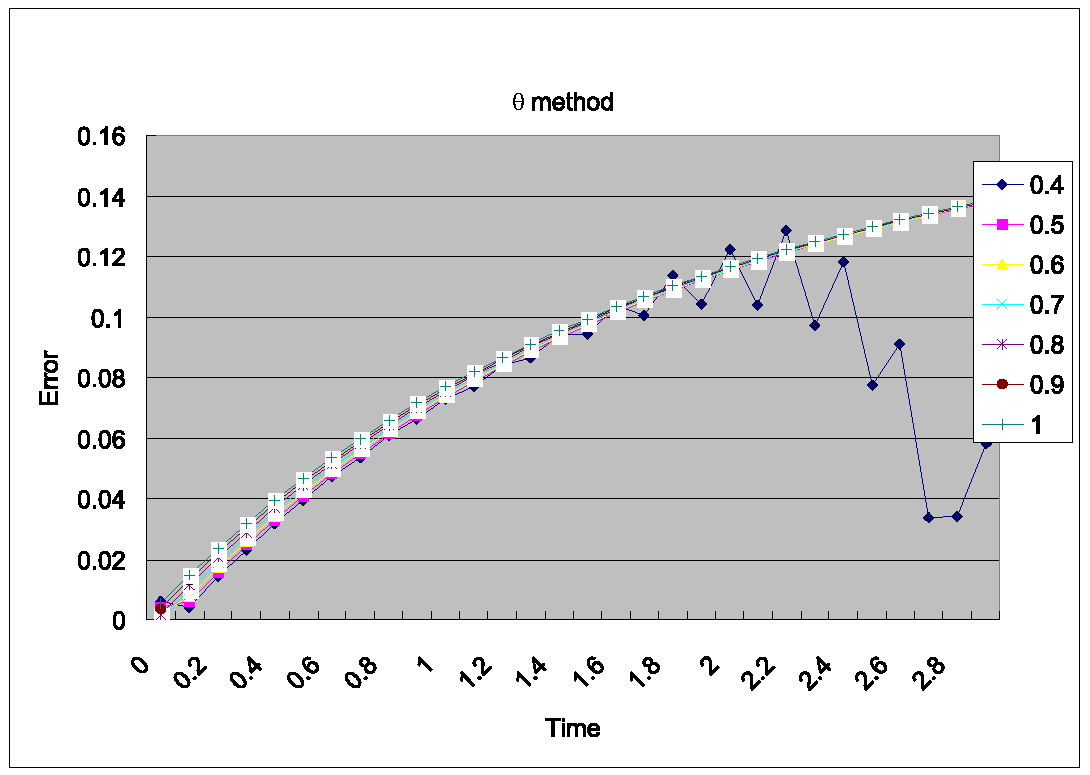
\includegraphics[height=6cm]{err02}
\end{center}
\caption{$\max_{x\in \Omega}|u_h^n(\theta)-u_{ex}(n\tau)|/\max_{x\in \Omega}|u_{ex}(n\tau)|$ at $n=0,1,\cdots,29$}
\label{fig:err02}
\end{figure}
We can see in Fig. \ref{fig:err02} that $u_h^n(\theta)$ become unstable at $\theta=0.4$, and figures are omitted in the case $\theta<0.4$.
\end{example}

\subsubsection{Convection}
The hyperbolic equation
\begin{eqnarray}
\label{eqn:conv}
\p_t u-\vec{\alpha} \cdot \nabla u=f;~~
\textrm{for a vector-valued function }\vec{\alpha},~
\p_t=\frac{\p}{\p t},
\end{eqnarray}
appear frequently in scientific problems, for example,
Navier-Stokes equation, Convection-Diffusion equation, etc.

In the case of 1-dimensional space, we can easily find the general solution
$(x,t)\mapsto u(x,t)=u^0(x-\alpha t)$ of the following equation, if $\alpha$ is constant,
\begin{eqnarray}
\label{eqn:conv0}
\p_t u +\alpha\p_x u=0,\qquad u(x,0)=u^0(x),
\end{eqnarray}
because $\p_t u +\alpha\p_x u=-\alpha\dot{u}^0+a\dot{u}^0=0$,
where $\dot{u}^0=du^0(x)/dx$.
Even if $\alpha$ is not constant construction, the principle is similar.
One begins the ordinary differential equation
(with convention which $\alpha$
is prolonged by zero apart from $(0,L)\times (0,T)$):
\[
\dot{X}(\tau )=-\alpha(X(\tau ),\tau ),~~~\tau \in (0,t)\quad X(t)=x
\]%
In this equation $\tau$ is the variable and $x,t$ is parameters,
and we denote the solution by $X_{x,t}(\tau )$.
Then it is noticed that $(x,t)\rightarrow v(X(\tau ),\tau )$ in
$\tau=t$ satisfy the equation
\[
\p _{t}v+\alpha\p _{x}v=\p _{t}X\dot{v}+a\p _{x}X\dot{v}%
=0
\]%
and by the definition $\p _{t}X=\dot{X}=-\alpha$ and
$\p_{x}X=\p _{x}x$ in $\tau=t$, because
if $\tau =t$ we have $X(\tau )=x$.
The general solution of (\ref{eqn:conv0}) is thus the value of the boundary condition in $X_{x, t}(0)$,
it is has to say $u(x,t)=u^{0}(X_{x,t}(0))$ if $X_{x,t}(0)$ is on the
$x$ axis, $u(x,t)=u^{0}(X_{x,t}(0))$ if $X_{x,t}(0)$ is on the axis of
$t$.

In higher dimension $\Omega \subset R^{d},~d=2,3$, the equation of the
convection is written
\[
\p _{t}u+\vec{\alpha}\cdot \nabla u=0\hbox{ in }\Omega \times (0,T)
\]%
where  $\vec{a}(x,t)\in R^{d}$.
\freefempp implements the Characteristic-Galerkin method for convection operators. Recall that the equation (\ref{eqn:conv})
can be discretized as
\[
\frac{Du}{Dt} = f\;\;\textrm{i.e. }\frac{du}{dt}\left( {X(t),t} \right) = f\left(X( t ),t \right)\textrm{  where  }\frac{dX}{dt}( t ) = \vec \alpha( {X(t),t})
\]
where $D$  is  the total derivative operator.
So a good scheme is one step of backward
convection by the method of Characteristics-Galerkin
\begin{eqnarray}
\label{eqn:Charac}
\frac{1}{{\tau }}\left(u^{m + 1}(x) - u^m(X^m(x))\right) = f^m (x)
\end{eqnarray}
where $X^m (x)$ is an approximation of the solution at $t = m\tau $
of the ordinary differential equation
\[
\frac{d\vec{X}}{dt}(t) = \vec{\alpha}^m(\vec{X}(t)),\, \vec{X}((m + 1)\tau ) = x.
\]
where $\vec{\alpha}^m(x)=(\alpha_1(x,m\tau ),\alpha_2(x,m\tau ))$.
Because, by Taylor's expansion, we have
\begin{eqnarray}
\label{eqn:conv1}
u^m(\vec {X}(m\tau ))&=&
u^m(\vec{X}((m+1)\tau )) -
\tau \sum_{i=1}^d \frac{\p u^m}{\p x_i}(\vec{X}((m+1)\tau ))
\frac{\p X_i}{\p t}((m+1)\tau )
+o(\tau )\nonumber\\
&=&u^m(x)-\tau \vec{\alpha}^m(x)\cdot \nabla u^m(x)+o(\tau )
\end{eqnarray}
where $X_i(t)$ are the i-th component of $\vec{X}(t)$,
$u^m(x)=u(x,m\tau )$
and we used the chain rule and $x=\vec{X}((m+1)\tau )$.
From (\ref{eqn:conv1}), it follows that
\begin{eqnarray}
u^m(X^m(x))=u^m(x)-\tau \vec{\alpha}^m(x)\cdot \nabla u^m(x)+o(\tau ).
\end{eqnarray}
Also we apply Taylor's expansion for
$t\mapsto u^m(x-\vec{\alpha}^m(x)t),\, 0\le t\le \tau $, then
\[
u^m(x-\vec{\alpha}\tau )=u^m(x)-\tau \vec{\alpha}^m(x)\cdot \nabla u^m(x)+o(\tau ).
\]
Putting
\[
\ttCC{@convect}\left( {\vec{\alpha},\tau ,u^m } \right)
= u^m \left(x - \vec{\alpha}^m\tau  \right),
\]
we can get the approximation
\[
u^m \left( {X^m( x )} \right) \approx
{\ttCC{@convect}}\left( {[a_1^m ,a_2^m],\tau ,u^m } \right)\;\;
\textrm{by }x = X((m + 1)\tau ).
\]

A classical convection problem is that of the ``rotating bell''
(quoted from \cite{Lucquin}[p.16]).
Let $\Omega$ be the unit disk centered at 0,
with its center rotating with speed
$\alpha_1 = y,\, \alpha_2 = -x$
We consider the problem (\ref{eqn:conv}) with $f=0$ and the initial condition
$u(x,0)=u^0(x)$, that is, from (\ref{eqn:Charac})
\begin{eqnarray*}
u^{m + 1}(x) = u^m(X^m(x))\approx \texttt{convect}(\vec{\alpha},\tau ,u^m).
\end{eqnarray*}
The exact solution is $u(x, t) = u(\vec{X}(t))$
where $\vec{X}$ equals $x$
rotated around the origin by an angle $\theta = -t$ (rotate in clockwise).
So, if $u^0$ in a 3D perspective
looks like a bell, then $u$ will have exactly the same shape, but rotated by the
same amount.
The program consists in solving the equation until $T = 2\pi$, that is for a full
revolution and to compare the final solution with the initial one; they should
be equal.
\begin{example}[convect.edp]
\index{tutorial!convect.edp}
\bFF
@border C(t=0, 2*pi) { x=cos(t);  y=sin(t); }; // the unit circle
@mesh Th = @buildmesh(C(70));   // triangulates the disk
@fespace Vh(Th,P1);
Vh u0 = @exp(-10*((x-0.3)^2 +(y-0.3)^2));    // give $u^0$

@real dt = 0.17,t=0;       // time step
Vh a1 = -y, a2 = x;                   // rotation velocity
Vh u; // $u^{m+1}$
@for (@int m=0; m<2*pi/dt ; m++) {
    t += dt;
    u=@convect([a1,a2],dt,u0);  // $u^{m+1}=u^m(X^m(x))$
    u0=u;                      // m++
    @plot(u,cmm=" t="+t + ", min=" + u[].min + ", max=" +  u[].max,wait=0);
};
\eFF
\end{example}
\begin{note}
The scheme \texttt{convect} is unconditionally stable, then
the bell become lower and lower (the maximum of $u^{37}$ is $0.406$ as shown in Fig. \ref{BellLast}).
\twoplot[height=5cm]{BellInit}{BellLast}{$u^0=e^{-10((x-0.3)^2 +(y-0.3)^2)}$}{The bell at $t=6.29$}
\end{note}


\subsubsection{2D Black-Scholes equation for an European Put option}
In mathematical finance, an option on two assets is modeled by a Black-Scholes equations in two space
variables, (see for example Wilmott et al\cite{wilmott} or Achdou et al \cite{achdou}).
\begin{eqnarray}
\label{eqn:BS-1-1}
 &&\p _t u + \frac{{\left( {\sigma _1 x } \right)^2 }}{2}\frac{{\p ^2 u}}{{\p x^2 }} + \frac{{\left( {\sigma _2 y } \right)^2 }}{2}\frac{{\p ^2 u}}{{\p y^2 }} \\
 &&{\rm{      }} + \rho x y \frac{{\p ^2 u}}{{\p x \p y }} + rS_1 \frac{{\p u}}{{\p x }} + rS_2 \frac{{\p u}}{{\p y }} - rP = 0 \nonumber
\end{eqnarray}
which is to be integrated in $\left( {0,T} \right) \times \R^ +   \times \R^ +$
subject to, in the case of a put
\begin{eqnarray}
\label{eqn:BS-1-2}
u\left( {x , y ,T} \right) = \left( {K - \max \left( {x ,y } \right)} \right)^ +  .
\end{eqnarray}
Boundary conditions for this problem may not be so easy to device.
As in the one dimensional case the PDE contains boundary conditions on the axis
$x_1 = 0$ and on the axis $x_2 = 0$, namely two one dimensional Black-Scholes equations driven
respectively by the data $u\left( {0, + \infty ,T} \right)$
and $u\left( { + \infty ,0,T} \right)$.
These will be automatically accounted for because they are embedded in the PDE.
So if we do nothing in the variational form (i.e. if we take a Neumann boundary condition at
these two axis in the strong form) there will be no disturbance to these.
At infinity in one of the variable, as in 1D, it makes sense to impose $u=0$.
We take
\begin{eqnarray}
\label{eqn:BS-1-5}
\sigma _1  = 0.3,\;\;\sigma _2  = 0.3,\;\;\rho  = 0.3,\;\;r = 0.05,\;\;K = 40,\;\;T = 0.5
\end{eqnarray}
An implicit Euler scheme is used and a mesh adaptation is done every 10 time steps.
To have an unconditionally stable scheme, the first order terms are treated by the
Characteristic Galerkin method, which, roughly, approximates
\begin{eqnarray}
\label{eqn:BS-1-6}
\frac{{\p u}}{{\p t}} + a_1 \frac{{\p u}}{{\p x}} + a_2 \frac{{\p u}}{{\p y}} \approx \frac{1}{{\tau }}\left( {u^{n + 1} \left( x \right) - u^n \left( {x - \vec \alpha\tau } \right)} \right)
\end{eqnarray}
\begin{example}~
[BlackSchol.edp]\index{tutorial!BlackSchol.edp}

\bFF
// file BlackScholes2D.edp
@int m=30,L=80,LL=80, j=100;
@real sigx=0.3, sigy=0.3, rho=0.3, r=0.05, K=40, dt=0.01;
@mesh th=@square(m,m,[L*x,LL*y]);
@fespace Vh(th,P1);

Vh u=max(K-max(x,y),0.);
Vh xveloc, yveloc, v,uold;

@for (@int n=0; n*dt <= 1.0; n++)
{
  @if(j>20)  { th = @adaptmesh(th,u,verbosity=1,abserror=1,nbjacoby=2,
              err=0.001, nbvx=5000, omega=1.8, ratio=1.8, nbsmooth=3,
              splitpbedge=1, maxsubdiv=5,rescaling=1) ;
     j=0;
     xveloc = -x*r+x*sigx^2+x*rho*sigx*sigy/2;
     yveloc = -y*r+y*sigy^2+y*rho*sigx*sigy/2;
     u=u;
    };
  uold=u;
  @solve eq1(u,v,@init=j,@solver=LU) = @int2d(th)( u*v*(r+1/dt)
        + @dx(u)*@dx(v)*(x*sigx)^2/2 + @dy(u)*@dy(v)*(y*sigy)^2/2
        + (@dy(u)*@dx(v) + @dx(u)*@dy(v))*rho*sigx*sigy*x*y/2)
        - @int2d(th)( v*convect([xveloc,yveloc],dt,w)/dt) + @on(2,3,u=0);

  j=j+1;
};
@plot(u,wait=1,value=1);

\eFF
Results are shown on Fig. \ref{blackScholesE}).
\label{blackScholesE}
\twoplot[height=8cm]{BSth}{BSval}{The adapted triangulation}{The level line of the European basquet put option}
\end{example}

\subsection{Navier-Stokes Equation}

\subsubsection{Stokes and Navier-Stokes}

The Stokes equations are: for a given $\vec{f}\in L^2(\Omega)^2$,
\index{stokes}
\Blue{
\begin{equation} \label{eqn:Stokes}
    \left.\begin{array}{cl}
 -\Delta \vec{u}+\nabla p & =\vec{f} \\
 \nabla\cdot \vec{u} &=0
 \end{array}\right\}\quad \hbox{ in }\Omega
\end{equation}}
where $\vec{u}=(u_1,u_2)$ is the velocity vector and $p$ the pressure.
For simplicity, let us choose Dirichlet boundary conditions
on the velocity,  $\vec{u}=\vec{u}_{\Gamma}$ on $\Gamma$.

In Temam [Theorem 2.2], there ia a weak form of (\ref{eqn:Stokes}):
Find $\vec{v}=(v_1,v_2)\in \vec{V}(\Omega)$
\[
\vec{V}(\Omega)=\{\vec{w}\in H^1_0(\Omega)^2|\; \textrm{div}\vec{w}=0\}
\]
which satisfy
\[
\sum_{i=1}^2\int_{\Omega}\nabla u_i\cdot \nabla v_i=\int_{\Omega}\vec{f}\cdot \vec{w}
\quad \textrm{for all }v\in V
\]
Here it is used the existence
$p\in H^1(\Omega)$ such that $\vec{u}=\nabla p$, if
\[
\int_{\Omega}\vec{u}\cdot \vec{v}=0\quad \textrm{for all }\vec{v}\in
V
\]
\medskip

Another weak form is derived as follows: We put
\begin{eqnarray*}
\vec{V}=H^1_0(\Omega)^2;\quad
W=\left\{q\in L^2(\Omega)\left|\; \int_{\Omega}q=0\right.\right\}
\end{eqnarray*}
By multiplying the first equation in (\ref{eqn:Stokes}) with $v\in V$ and the
second with $q\in W$, subsequent integration over $\Omega$, and an
application of Green's formula, we have
\begin{eqnarray*}
\int_{\Omega}\nabla\vec{u}\cdot \nabla\vec{v}-\int_{\Omega}\textrm{div}\vec{v}\, p
&=&\int_{\Omega}\vec{f}\cdot\vec{v}\\
\int_{\Omega}\textrm{div}\vec{u}\, q&=&0
\end{eqnarray*}
This yields the weak form of (\ref{eqn:Stokes}):
Find $(\vec{u},p)\in \vec{V}\times W$ such that
\begin{eqnarray}
\label{eqn:wStokes-1}
a(\vec{u},\vec{v})+b(\vec{v},p)&=&(\vec{f},\vec{v})\\
\label{eqn:wStokes-2}
b(\vec{u},q)&=&0
\end{eqnarray}
for all $(\vec{v},q)\in V\times W$, where
\begin{eqnarray}
\label{eqn:Stokes-a}
a(\vec{u},\vec{v})&=&\int_{\Omega}\nabla \vec{u}\cdot \nabla\vec{v}
=\sum_{i=1}^2\int_{\Omega}\nabla u_i\cdot \nabla v_i\\
\label{eqn:Stokes-b}
b(\vec{u},q)&=&-\int_{\Omega}\textrm{div}\vec{u}\, q
\end{eqnarray}

Now, we consider finite element spaces $\vec{V}_h\subset \vec{V}$ and $W_h\subset W$,
and we assume the following basis functions
\begin{eqnarray*}
&&\vec{V}_h=V_h\times V_h,\quad
V_h=\{v_h|\; v_h=v_1\phi_1+\cdots +v_{M_V}\phi_{M_V}\},\\
&&W_h=\{q_h|\; q_h=q_1\varphi_1+\cdots +q_{M_W}\varphi_{M_W}\}
\end{eqnarray*}
The discrete weak form is:
Find $(\vec{u}_{h},p_{h}) \in \vec{V}_{h} \times W_{h}$ such that
\Blue{
\begin{equation} \label{eqn:vfStokes}
    \begin{array}{cll}
   a(\vec{u}_h,\vec{v}_h)+b(\vec{v}_h,p)  &= (\vec{f},\vec{v}_h) ,
      &\forall \vec{v}_{h} \in \vec{V}_{h} \\
    b(\vec{u}_h,q_h)&= 0,
     &\forall q_{h} \in W_{h}
    \end{array}
\end{equation}}
\begin{note}
Assume that:
\begin{enumerate}
  \item There is a constant $\alpha_h>0$ such that
  \[
  a(\vec{v}_h,\vec{v}_h)\ge \alpha\| \vec{v}_h\|_{1,\Omega}^2\quad \textrm{for all }\vec{v}_h\in Z_h
  \]
  where
  \[
  Z_h=\{\vec{v}_h\in \vec{V}_h|\; b(\vec{w}_h,q_h)=0\quad \textrm{for all }q_h\in W_h\}
  \]
  \item There is a constant $\beta_h>0$ such that
  \[
  \sup_{\vec{v}_h\in \vec{V}_h}\frac{b(\vec{v}_h,q_h)}{\| \vec{v}_h\|_{1,\Omega}}
  \ge \beta_h\| q_h\|_{0,\Omega}\quad \textrm{for all }q_h\in W_h
  \]
\end{enumerate}
  Then we have an unique solution $(\vec{u}_h,p_h)$ of (\ref{eqn:vfStokes})
  satisfying
  \[
  \| \vec{u}-\vec{u}_h\|_{1,\Omega}+\| p-p_h\|_{0,\Omega}
  \le C\left(
  \inf_{\vec{v}_h\in \vec{V}_h}\| u-v_h\|_{1,\Omega}
  +\inf_{q_h\in W_h}\| p-q_h\|_{0,\Omega}\right)
  \]
  with a constant $C>0$ (see e.g. \cite[Theorem 10.4]{RT93}).
\end{note}
Let us denote that
\begin{eqnarray}
A&=&(A_{ij}),\, A_{ij}=\int_{\Omega}\nabla \phi_j\cdot \nabla \phi_i\qquad
i,j=1,\cdots,M_{\vec{V}}\\
\vec{B}&=&(Bx_{ij},By_{ij}),\,
Bx_{ij}=-\int_{\Omega}\p \phi_j/\p x\, \varphi_i\qquad
By_{ij}=-\int_{\Omega}\p \phi_j/\p y\, \varphi_i\nonumber\\
&&\qquad i=1,\cdots,M_W;j=1,\cdots,M_V\nonumber
\end{eqnarray}
then (\ref{eqn:vfStokes}) is written by
\begin{eqnarray}
\left(
\begin{array}{cc}
\vec{A}&\vec{\vec{B}}^*\\
\vec{B}&0
\end{array}
\right)
\left(
\begin{array}{cc}
\vec{U}_h\\
\{p_h\}
\end{array}
\right)
=
\left(
\begin{array}{cc}
\vec{F}_h\\
0
\end{array}
\right)
\end{eqnarray}
where
\begin{eqnarray*}
&&\vec{A}=\left(
\begin{array}{cc}
A&0\\
0&A
\end{array}
\right)
\qquad
\vec{B}^*=\left\{
\begin{array}{c}
Bx^T\\
By^T
\end{array}
\right\}
\qquad
\vec{U}_h=\left\{
\begin{array}{c}
\{u_{1,h}\}\\
\{u_{2,h}\}
\end{array}
\right\}
\qquad
\vec{F}_h=\left\{
\begin{array}{c}
\{\textstyle{\int_{\Omega}f_1\phi_i}\}\\
\{\textstyle{\int_{\Omega}f_2\phi_i}\}
\end{array}
\right\}
\end{eqnarray*}

\textbf{Penalty method:} This method consists of replacing (\ref{eqn:vfStokes}) by a more regular problem: Find
$(\vec{v}_h^{\epsilon},p_h^{\epsilon})\in \vec{V}_h\times \tilde{W}_{h}$ satisfying
\Blue{
\begin{equation} \label{eqn:PvfStokes}
    \begin{array}{cll}
   a(\vec{u}_h^\epsilon,\vec{v}_h)+b(\vec{v}_h,p_h^{\epsilon})  &= (\vec{f},\vec{v}_h) ,
      &\forall \vec{v}_{h} \in \vec{V}_{h} \\
    b(\vec{u}_h^{\epsilon},q_h)-\epsilon(p_h^{\epsilon},q_h)&= 0,
     &\forall q_{h} \in \tilde{W}_{h}
    \end{array}
\end{equation}}
where $\tilde{W}_h\subset L^2(\Omega)$. Formally, we have
\[
\textrm{div}\vec{u}_h^{\epsilon}=\epsilon p_h^{\epsilon}
\]
and the corresponding algebraic problem
\begin{eqnarray*}
\left(
\begin{array}{cc}
\vec{A}&B^*\\
B&-\epsilon I
\end{array}
\right)
\left(
\begin{array}{cc}
\vec{U}_h^{\epsilon}\\
\{p_h^{\epsilon}\}
\end{array}
\right)
=
\left(
\begin{array}{cc}
\vec{F}_h\\
0
\end{array}
\right)
\end{eqnarray*}
\begin{note}
We can eliminate $p_h^\epsilon=(1/\epsilon)BU_h^{\epsilon}$ to obtain
\begin{eqnarray}
\label{eqn:StiffPvfStokes}
(A+(1/\epsilon)B^*B)\vec{U}_h^{\epsilon}=\vec{F}_h^{\epsilon}
\end{eqnarray}
Since the matrix $A+(1/\epsilon)B^*B$ is symmetric, positive-definite, and sparse, (\ref{eqn:StiffPvfStokes}) can be solved by known technique.
There is a constant $C>0$ independent of $\epsilon$ such that
\[
\|\vec{u}_h-\vec{u}_h^\epsilon\|_{1,\Omega}+
\|p_h-p_h^{\epsilon}\|_{0,\Omega}\le C\epsilon
\]
(see e.g. \cite[17.2]{RT93})
\end{note}

\begin{example}[Cavity.edp]

The driven cavity flow problem is solved first at zero Reynolds number
(Stokes flow) and then at Reynolds 100.  \index{fluid}The
velocity pressure formulation is used first and then the calculation
is repeated with the stream function vorticity formulation.

We solve the driven cavity problem by the penalty method (\ref{eqn:PvfStokes}) \index{Stokes} where
 $\vec{u}_{\Gamma}\cdot \vec{n}=0$ and $\vec{u}_{\Gamma}\cdot \vec{s}
=1$ on the top boundary and zero elsewhere ( $\vec{n}$ is the unit normal to $\Gamma$, and $\vec{s}$ the unit tangent to $\Gamma$).
\\
The mesh is constructed by
\bFF
@mesh Th=@square(8,8);
\eFF

We use a classical Taylor-Hood element technic to solve the problem:
\\\\
The velocity is approximated with the $P_{2}$ FE ( $X_{h}$ space), and the
the pressure is approximated with the $P_{1}$ FE ( $M_{h}$ space),
\\\\
where
\Blue{
$$  X_{h} = \left\{ \vec{v} \in H^{1}(]0,1[^2) \left|\; \forall K \in \mathcal{T}_{h}
\quad v_{|K} \in
P_{2} \right.\right\}$$} and
\Blue{$$  M_{h} = \left\{ v \in H^{1}(]0,1[^2) \left|\; \forall K \in \mathcal{T}_{h}
\quad v_{|K} \in
P_{1} \right.\right\}$$}

The FE spaces and functions  are constructed by

\bFF
@fespace Xh(Th,@P2); //  definition of the velocity component space
@fespace Mh(Th,@P1);  //  definition of the pressure space
Xh u2,v2;
Xh u1,v1;
Xh p,q;
\eFF

The Stokes operator is implemented as a system-solve for the velocity
$(u1,u2)$ and the pressure $p$.  The test function  for the velocity is $(v1,v2)$
and $q$ for the pressure, so the variational form (\ref{eqn:vfStokes}) in freefem
language is:
\bFF
@solve Stokes (u1,u2,p,v1,v2,q,solver=Crout) =
    @int2d(Th)( ( dx(u1)*dx(v1) + dy(u1)*dy(v1)
            +  dx(u2)*dx(v2) + dy(u2)*dy(v2) )
            - p*q*(0.000001)
            - p*dx(v1) - p*dy(v2)
            - dx(u1)*q - dy(u2)*q
           )
  + @on(3,u1=1,u2=0)
  + @on(1,2,4,u1=0,u2=0); // see \refSec{Square} for labels 1,2,3,4
\eFF
Each unknown has its own boundary conditions.
\\\\

If the \index{streamlines}streamlines are required, they can be
computed by finding $\psi$ such that rot$\psi=u$ or better,
\Blue{$$-\Delta\psi=\nabla\times u$$}
\bFF
Xh psi,phi;

@solve streamlines(psi,phi) =
      @int2d(Th)( dx(psi)*dx(phi) + dy(psi)*dy(phi))
   +  @int2d(Th)( -phi*(dy(u1)-dx(u2)))
   +  @on(1,2,3,4,psi=0);
\eFF

\bigskip

Now the Navier-Stokes equations are solved
\eq{
    {\p {u}\over\p t} +u\cdot\nabla u-\nu \Delta u+\nabla p=0,~~~ \nabla\cdot u=0
}
with the same boundary conditions and with initial conditions $u=0$.

This is implemented by using the convection operator \texttt{convect} for the term
${\p u\over\p t} +u\cdot\nabla u$, giving a discretization in time
\Blue{\index{Navier-Stokes}
\begin{equation}
    \label{eq Navier Stokes carac}
\begin{array}{cl}
\frac{1}{\tau } (u^{n+1}-u^n\circ X^n) -\nu\Delta u^{n+1} + \nabla p^{n+1} &=0,\\
 \nabla\cdot u^{n+1} &= 0
 \end{array}
\end{equation}
}
The term $u^n\circ X^n(x)\approx u^n(x-u^n(x)\tau )$ will be
computed by the operator ``convect" \index{convect} , so we obtain
\bFF
int i=0;
@real  nu=1./100.;
@real dt=0.1;
@real alpha=1/dt;

Xh up1,up2;

@problem  NS (u1,u2,p,v1,v2,q,solver=Crout,init=i) =
    @int2d(Th)(
             alpha*( u1*v1 + u2*v2)
            + nu * ( dx(u1)*dx(v1) + dy(u1)*dy(v1)
            +  dx(u2)*dx(v2) + dy(u2)*dy(v2) )
            - p*q*(0.000001)
            - p*dx(v1) - p*dy(v2)
            - dx(u1)*q - dy(u2)*q
           )
  + @int2d(Th) ( -alpha*
       convect([up1,up2],-dt,up1)*v1 -alpha*convect([up1,up2],-dt,up2)*v2 )
  + @on(3,u1=1,u2=0)
  + @on(1,2,4,u1=0,u2=0)
;

@for (i=0;i<=10;i++)
 {
   up1=u1;
   up2=u2;
   NS;
   @if ( !(i % 10))  // plot every 10 iteration
    @plot(coef=0.2,cmm=" [u1,u2] and p  ",p,[u1,u2]);
 } ;
\eFF
Notice that the stiffness matrices are \index{Reusable matrices}
reused (keyword
\texttt{init=i})
\end{example}

\subsubsection{\setS{Uzawa} Conjugate Gradient}
We solve Stokes problem without penalty.
The classical iterative method of Uzawa is described by the algorithm
(see e.g.\cite[17.3]{RT93}):
\begin{description}
  \item[Initialize:] Let $p_h^0$ be an arbitrary chosen element of
  $L^2(\Omega)$.
  \item[Calculate $\vec{u}_h$:] Once $p_h^n$ is known, $\vec{v}_h^n$ is the solution of
  \[
  \vec{u}_h^n = A^{-1}(\vec{f}_h-\vec{B}^*p_h^n)
  \]
  \item[Advance $p_h$:] Let $p_h^{n+1}$ be defined by
  \[
  p_h^{n+1}=p_h^n+\rho_n\vec{B}\vec{u}_h^n
  \]
\end{description}
There is a constant $\alpha>0$ such that $\alpha\le \rho_n\le 2$ for each $n$,
then $\vec{u}_h^n$ converges to the solution $\vec{u}_h$, and then
$B\vec{v}_h^n\to 0$ as $n\to \infty$ from the \emph{Advance $p_h$}.
This method in general converges quite slowly.

First we define mesh, and the Taylor-Hood \index{Taylor-Hood}  approximation.
So $X_{h}$  is the velocity space, and $M_{h}$ is the pressure space.
\begin{example}[StokesUzawa.edp]~
\index{tutorial!StokesUzawa.edp}
\bFF
@mesh Th=@square(10,10);
@fespace Xh(Th,@P2),Mh(Th,@P1);
Xh u1,u2,v1,v2;
Mh p,q,ppp;  //  ppp is a working pressure
\eFF

\bFF
@varf bx(u1,q) = @int2d(Th)( -(dx(u1)*q));
@varf by(u1,q) = @int2d(Th)( -(dy(u1)*q));
@varf a(u1,u2)= @int2d(Th)(  dx(u1)*dx(u2) + dy(u1)*dy(u2) )
                    +  on(3,u1=1)  +  @on(1,2,4,u1=0) ;
//  remark:  put the \ttCC{@on(3,u1=1)} before  \ttCC{@on(1,2,4,u1=0)}
//  because we want zero on intersection %\index{on!intersection}

@matrix A= a(Xh,Xh,solver=CG);
@matrix Bx= bx(Xh,Mh);  // $\vec{B}=(Bx\quad By)$
@matrix By= by(Xh,Mh);

Xh bc1; bc1[] = a(0,Xh);  //  boundary condition contribution  on u1
Xh bc2; bc2   = O ;       //  no boundary condition contribution on u2
Xh b;
\eFF

$p_h^n\to \vec{B}A^{-1}(-\vec{B}^*p_h^n)=-\textrm{div}\vec{u}_h$
is realized as
the function \emph{\texttt{divup}}.
\bFF
@func @real[@int] divup(@real[@int] @& pp)
{
   //  compute u1(pp)
   b[]  = Bx'*pp; b[] *=-1; b[] += bc1[] ;    u1[] = A^-1*b[];
   //  compute u2(pp)
   b[]  = By'*pp; b[] *=-1; b[] += bc2[] ;    u2[] = A^-1*b[];
   //  $\vec{u}^n=A^{-1}(Bx^Tp^n\quad By^Tp^n)^T$ \hfilll
   ppp[] =   Bx*u1[];   // $  ppp= Bx u_{1} $
   ppp[] +=  By*u2[];   // $   \quad   +  By u_{2} $
   @return ppp[] ;
};
\eFF

 Call now the conjugate gradient algorithm:

\bFF
p=0;q=0; // $p_h^0 = 0$
@LinearCG(divup,p[],eps=1.e-6,nbiter=50); // $p_h^{n+1}=p_h^n+\vec{B}\vec{u}_h^n$
// if $n> 50$ or $|p_h^{n+1}-p_h^n|\le 10^{-6}$, then the loop end. \hfilll
divup(p[]); // compute the final solution

@plot([u1,u2],p,wait=1,value=true,coef=0.1);
\eFF
\end{example}

\subsubsection{NSUzawaCahouetChabart.edp}

 In this example we solve the Navier-Stokes \index{Navier-Stokes} equation,
 in the driven-cavity,
 with the Uzawa  algorithm preconditioned by the Cahouet-Chabart method.

 The idea of the preconditioner is that in a periodic domain, all
 differential operators commute and  the  Uzawa algorithm comes to solving the
 linear operator  $ \nabla. ( (\alpha Id + \nu \Delta)^{-1} \nabla$,
 where $ Id $ is the identity operator.
 So  the preconditioer suggested is $ \alpha \Delta^{-1} + \nu Id$.
\\\\
To implement this, we reuse the previous example, by including \index{include} a file.
Then we define the time step $ \Delta t$, viscosity, and new variational form and matrix.

\begin{example}[NSUzawaCahouetChabart.edp]~
\index{tutorial!NSUzawaCahouetChabart.edp}
\bFF
@include "StokesUzawa.edp" // include the Stokes part
@real dt=0.05, alpha=1/dt;  // $ \Delta t$

@cout << " alpha = " << alpha;
@real xnu=1./400; // viscosity $ \nu = {\hbox{Reynolds number}}^{-1} $

//  the new variational form with mass term \index{varf}
@varf at(u1,u2)= @int2d(Th)( xnu*dx(u1)*dx(u2)
                        + xnu*dy(u1)*dy(u2) + u1*u2*alpha  )
                        +  @on(1,2,4,u1=0)  + @on(3,u1=1) ;

A = at(Xh,Xh,solver=CG);  //  change the matrix \index{matrix!=}\index{matrix!solver=}

//  set the 2 convect variational form \index{qforder=} \index{convect}
@varf  vfconv1(uu,vv)  = @int2d(Th,qforder=5) (@convect([u1,u2],-dt,u1)*vv*alpha);
@varf  vfconv2(v2,v1)  = @int2d(Th,qforder=5) (@convect([u1,u2],-dt,u2)*v1*alpha);

@int idt;       // index of of time set
@real temps=0;  // current time

Mh pprec,prhs;
@varf vfMass(p,q) = int2d(Th)(p*q);
@matrix MassMh=vfMass(Mh,Mh,solver=CG);

@varf vfLap(p,q)  = int2d(Th)(dx(pprec)*dx(q)+dy(pprec)*dy(q) + pprec*q*1e-10);
@matrix LapMh= vfLap(Mh,Mh,solver=Cholesky);
\eFF

 The function to define the preconditioner

\bFF
@func real[int]  CahouetChabart(real[int] & xx)
{  //  xx = $ \int (div u) w_i$
   //   $ \alpha LapMh ^{-1}  + \nu MassMh^{-1} $
   pprec[]= LapMh^-1* xx;
   prhs[] =  MassMh^-1*xx;
   pprec[] = alpha*pprec[]+xnu* prhs[];
   @return pprec[];
};
\eFF

The loop in time.
Warning with the stop test of the conjugate gradient, because
we start from the previous solution and the end the previous solution
is close to the final solution, don't take a relative  stop test to
the first residual, take an absolute stop test ( negative here)
\index{stop test!absolue}
\bFF
for (idt = 1; idt < 50; idt++)
 {
   temps += dt;
   cout << " --------- temps " << temps << " \n ";
   b1[] =  vfconv1(0,Xh);
   b2[] =  vfconv2(0,Xh);
   cout << "  min b1 b2  " << b1[].min << " " << b2[].min << endl;
   cout << "  max b1 b2  " << b1[].max << " " << b2[].max << endl;
   // call Conjugate Gradient with preconditioner '
   //  warning eps < 0 => absolue stop test \index{precon=}
   LinearCG(divup,p[],eps=-1.e-6,nbiter=50,precon=CahouetChabart);
   divup(p[]);   //  computed the velocity

   plot([u1,u2],p,wait=!(idt%10),value= 1,coef=0.1);
 }
\eFF
\end{example}
\begin{figure}[http]
\label{cahouetchabart}\begin{center}
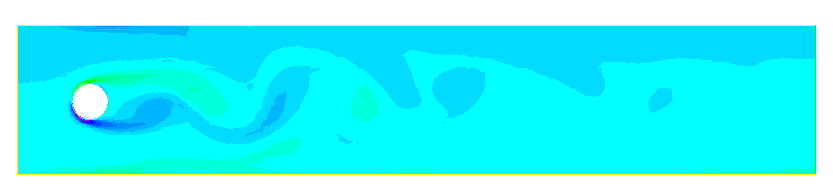
\includegraphics[width=8cm]{NScahouetChabart}
\caption{Solution of the cavity driven problem at Reynolds number 400 with the
Cahouet-Chabart algorithm.}
\end{center}
\end{figure}

\subsection{Variational  inequality}
We present, a classical examples of variational inequality.

Let us denote  $\mathcal{C} = \{ u\in H^1_0(\Omega), u \le g \}$

The problem is :

$$
 u = arg \min_{u\in \mathcal{C}}  J(u) = \frac{1}{2} \int_\Omega \nabla u . \nabla u - \int_\Omega f u
$$
where $f$ and $g$ are given function.

The solution is a projection on the convex $\mathcal{C}$ of $f^\star$
for the scalar product $((v,w)) = \int_\Omega \nabla v . \nabla w$ of
$  H^1_0(\Omega)$
where $ {f^\star} $ is solution of $ ((f^\star, v )) = \int_\Omega f v, \forall v \in  H^1_0(\Omega)$.
The projection on a convex satisfy clearly
$\forall v \in \mathcal{C}, \quad   (( u -v ,  u - \tilde{f}  )) \leq 0   $,
and after expanding, we get the classical inequality
$$\forall v \in \mathcal{C}, \quad   \int_\Omega \nabla(u -v) \nabla  u  \leq  \int_\Omega   (u-v) f .   $$

We can also rewrite the problem as a saddle point problem

Find $\lambda, u$ such that:
$$
  \max_{\lambda\in L^2(\Omega), \lambda\geq 0}  \min_{u\in H^1_0(\Omega)}  \mathcal{L}(u,\lambda) = \frac{1}{2} \int_\Omega \nabla u . \nabla u - \int_\Omega f u  + \int_{\Omega} \lambda (u-g)^+
$$
where $((u-g)^+ = max(0,u-g) $

This saddle point problem is equivalent to find $ u, \lambda $ such that:
\begin{equation}
 \left\{
\begin{array}{cc}
\displaystyle \int_\Omega \nabla u . \nabla v + \lambda v^+ \,d\omega= \int_\Omega f u  , &\forall v \in H^1_0(\Omega) \cr
\displaystyle \int_\Omega   \mu (u-g)^+ = 0  , & \forall \mu \in L^2(\Omega) , \mu \geq 0, \lambda \geq 0,
 \end{array}\right.\label{eq:iq1}
\end{equation}


A algorithm to solve the previous problem is:

\begin{enumerate}
\item k=0, and choose, $\lambda_0$ belong $ H^{-1}(\Omega)$
\item loop on $ k = 0, .....$
 \begin{enumerate}
\item  set $ \mathcal{I}_{k} = \{ x \in \Omega / \lambda_{k} + c * ( u_{k+1} - g)  \leq 0 \} $
\item  $ V_{g,k+1} = \{ v\in H^1_0(\Omega) / v = g $   on ${I}_{k} \}$,
\item  $ V_{0,k+1} = \{ v\in  H^1_0(\Omega) / v = 0$ on ${I}_{k} \}$,
 \item Find  $ u_{k+1} \in V_{g,k+1} $ and  $\lambda_{k+1} \in H^{-1}(\Omega)$ such that
 $$
 \left\{\begin{array}{cc}
 \displaystyle  \int_\Omega \nabla u_{k+1}. \nabla v_{k+1}   \,d\omega = \int_\Omega f v_{k+1}  , &\forall v_{k+1} \in  V_{0,k+1} \cr
 \displaystyle  <\lambda_{k+1},v>  =  \int_\Omega \nabla u_{k+1}. \nabla v  -  f v \,d\omega &
  \end{array}\right.
 $$
 where $<,>$ is the duality bracket between $ H^{1}_0(\Omega)$ and  $ H^{-1}(\Omega)$, and $c$
is  a penalty constant (large enough).
\end{enumerate}

\end{enumerate}
You can find all the mathematic  about this algorithm in \cite{ItoKunisch}.

Now how to do that in \texttt{FreeFem++}

The full example is:
\begin{example}[VI.edp]
\index{tutotial!VI.edp}
\bFF

@mesh Th=square(20,20);
@real eps=1e-5;
@fespace Vh(Th,P1);     // P1 FE space
@int n = Vh.ndof; // number of Degree of freedom
@Vh uh,uhp;              // solution and previous one
@Vh Ik; //  to def the set where the containt is reached.
@real[int] rhs(n); // to store the right and side of the equation
@real c=1000;  // the penalty  parameter of the algoritm
@func f=1;         //  right hand side function
@func fd=0;         // Dirichlet   boundary condition function
Vh g=0.05;  // the discret function g

@real[int] Aii(n),Aiin(n); // to store the diagonal of the matrix 2 version

@real tgv = 1e30; // a huge value for exact penalization
// of boundary condition
//  the variatonal form of the problem: \hfilll
@varf a(uh,vh) =                    //  definition of  the problem
    int2d(Th)( dx(uh)*dx(vh) + dy(uh)*dy(vh) ) //  bilinear form
  - int2d(Th)( f*vh )                          //  linear form
  + on(1,2,3,4,uh=fd) ;                      //  boundary condition form


// two version of the matrix of the problem  \hfilll
@matrix A=a(Vh,Vh,tgv=tgv,solver=CG); // one changing
@matrix AA=a(Vh,Vh,solver:GC); // one for computing residual

 //  the mass Matrix construction: \hfilll
@varf vM(uh,vh) = int2d(Th)(uh*vh);
@matrix M=vM(Vh,Vh); // to do a fast computing of $L^2$ norm : sqrt( u'*(w=M*u))

Aii=A.diag; // get the diagonal of the matrix (appear in version 1.46-1)

rhs = a(0,Vh,tgv=tgv);
Ik =0;
uhp=-tgv; // previous value is
Vh lambda=0;
@for(int iter=0;iter<100;++iter)
{
  @real[int] b(n) ; b=rhs;  //  get a copy of the Right hand side
  @real[int] Ak(n); //  the complementary of Ik ( !Ik = (Ik-1))
  // Today  the operator Ik- 1. is not implement so we do:
  Ak= 1.; Ak  -= Ik[];  // build Ak  = ! Ik
  //  adding new locking  condition on b and on the diagonal if (Ik ==1 )
  b = Ik[] .* g[];      b *= tgv;     b  -=  Ak .* rhs;
  Aiin = Ik[] *  tgv;      Aiin  +=  Ak  .* Aii;  //set  Aii= tgv  $ i \in Ik $
  A.diag = Aiin; //  set the matrix diagonal  (appear in version 1.46-1)
  @set(A,solver=CG); // important to change preconditioning  for solving
  uh[] = A^-1* b;   //  solve the problem with more locking condition
  lambda[] = AA * uh[]; //  compute the residual ( fast with matrix)
  lambda[] += rhs; // remark rhs = $-\int f v $

  Ik = ( lambda + c*( g- uh)) < 0.;  // the new of locking value

   @plot(Ik, wait=1,cmm=" lock set ",value=1,ps="VI-lock.eps",fill=1 );
   @plot(uh,wait=1,cmm="uh",ps="VI-uh.eps");
   // trick to compute  $L^2$ norm of the variation (fast method)
      real[int] diff(n),Mdiff(n);
      diff= uh[]-uhp[];
      Mdiff = M*diff;
      real err = sqrt(Mdiff'*diff);
  @cout << "  || u_{k=1} - u_{k} ||_2 " << err << endl;
  @if(err< eps) @break; // stop test
  uhp[]=uh[] ; // set the previous solution
}
savemesh(Th,"mm",[x,y,uh*10]); // for medit plotting
\eFF
\end{example}

Remark, as you can see on this example, some vector , or matrix operator are not implemented
so a way is to skip the expression and we  use operator \texttt{+=},  \texttt{-=} to merge
the result.


\subsection{Domain decomposition}
We present, three classic examples, of domain decomposition
technique:
first, Schwarz algorithm with overlapping, second
Schwarz algorithm without  overlapping (also call Shur complement), and
last we show to use the conjugate gradient
to solve the boundary problem of the Shur complement.

\subsubsection{Schwarz Overlap Scheme}
\label{schwarz-overlap}
To solve
\eq{ -\Delta u =f,\; \hin\Omega=\Omega_1\cup\Omega_2\quad u|_\Gamma=0}
the Schwarz algorithm  runs like this
\Blue{
\begin{eqnarray*}
   -\Delta u^{n+1}_1&=&f\hin\Omega_1\quad
    u^{n+1}_1|_{\Gamma_1}=u^n_2\\
    -\Delta u^{n+1}_2&=&f\hin\Omega_2\quad
    u^{n+1}_2|_{\Gamma_2}=u^n_1
\end{eqnarray*}}
where $\Gamma_i$ is the boundary of $\Omega_i$ and on the
condition that $\Omega_1\cap\Omega_2\neq\emptyset$ and that $u_i$
are zero at iteration 1.
\\\\
Here we take $\Omega_1$ to be a quadrangle, $\Omega_2$ a disk and
we apply the algorithm starting from zero.
\begin{figure}[hbt]
\HLINE{\hss
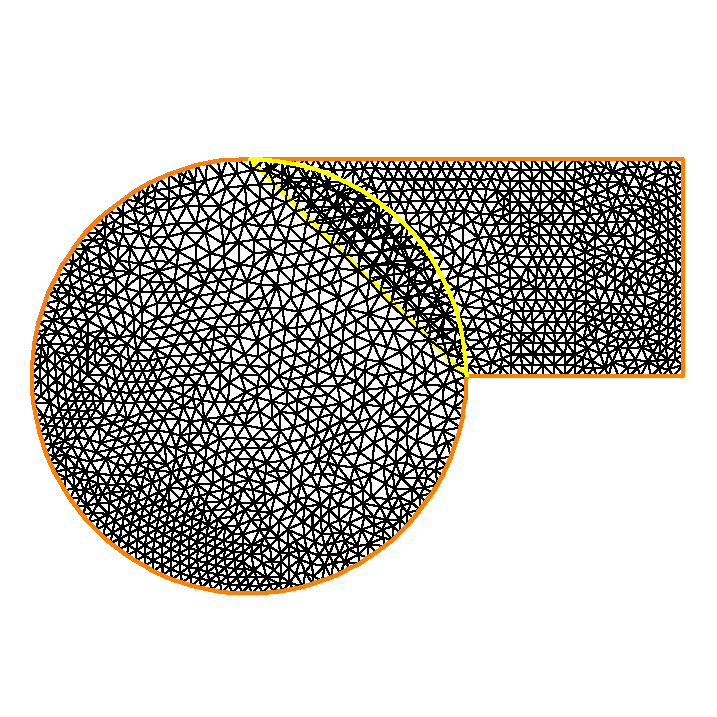
\includegraphics[width=6cm]{schwarz-th} \hss}
\caption{ The 2 overlapping mesh \texttt{TH} and \texttt{th}  }
\end{figure}

\begin{example}[Schwarz-overlap.edp]~
\index{tutorial!Schwarz-overlap.edp}
 \bFF
@int inside = 2;  //  inside boundary
@int outside = 1; //  outside boundary
@border a(t=1,2){x=t;y=0;label=outside;};
@border b(t=0,1){x=2;y=t;label=outside;};
@border c(t=2,0){x=t ;y=1;label=outside;};
@border d(t=1,0){x = 1-t; y = t;label=inside;};
@border e(t=0, pi/2){ x= cos(t); y = sin(t);label=inside;};
@border e1(t=pi/2, 2*pi){ x= cos(t); y = sin(t);label=outside;};
@int n=4;
@mesh th = @buildmesh( a(5*n) + b(5*n) + c(10*n) + d(5*n));
@mesh TH = @buildmesh( e(5*n) + e1(25*n) );
@plot(th,TH,wait=1);  //  to see the 2 meshes
\eFF

The space  and problem definition is :
\bFF
@fespace vh(th,@P1);
@fespace VH(TH,@P1);
vh u=0,v; VH U,V;
@int i=0;

@problem PB(U,V,init=i,solver=Cholesky) =
    @int2d(TH)( dx(U)*dx(V)+dy(U)*dy(V) )
  + @int2d(TH)( -V) + on(inside,U = u)  + @on(outside,U= 0 ) ;
@problem pb(u,v,init=i,solver=Cholesky) =
    @int2d(th)( dx(u)*dx(v)+dy(u)*dy(v) )
  + @int2d(th)( -v) + on(inside ,u = U) + @on(outside,u = 0 ) ;
\eFF
 The  calculation loop:
\bFF
@for ( i=0 ;i< 10; i++)
{
   PB;
   pb;
   @plot(U,u,wait=true);
};
\eFF
\end{example}

\begin{figure}[hbt]
\HLINE{\hss
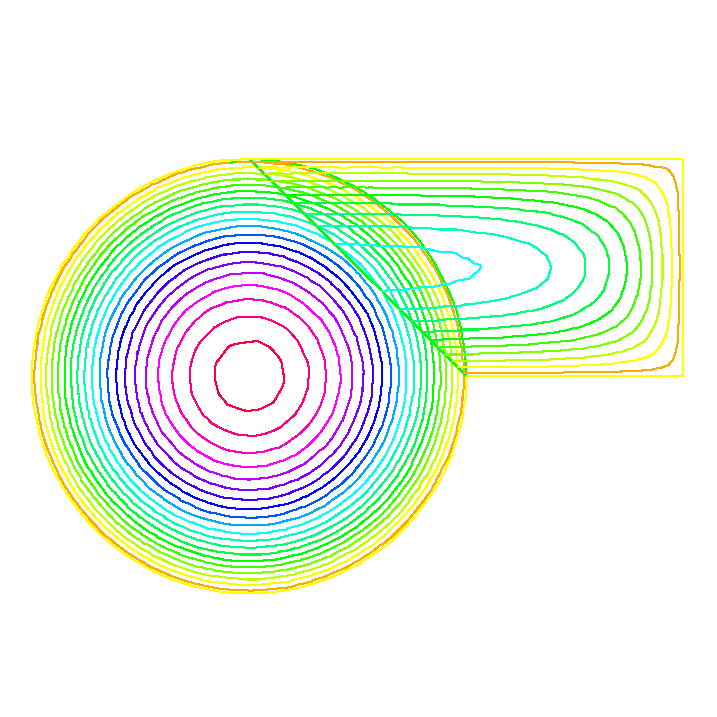
\includegraphics[width=6cm]{schwarz-u0}
\hss
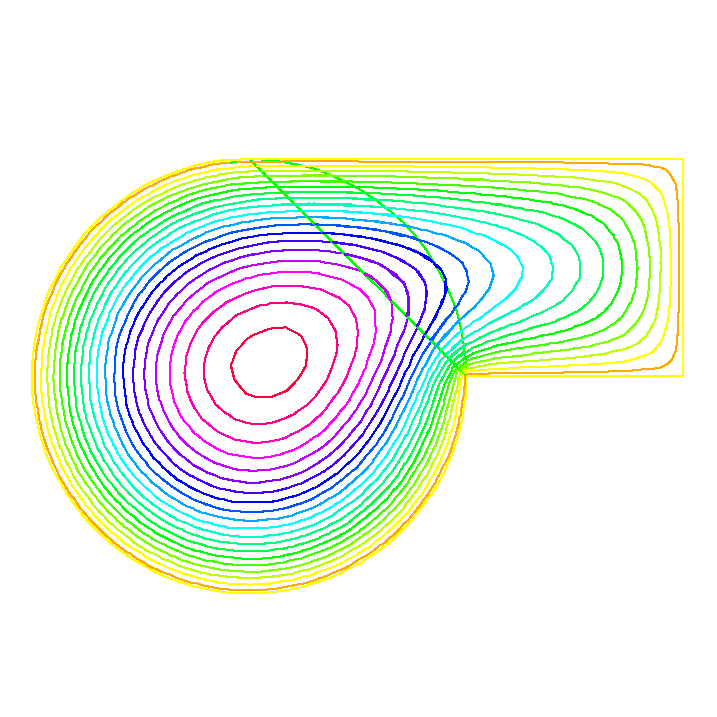
\includegraphics[width=6cm]{schwarz-u} }
\caption{  Isovalues of the solution at  iteration 0  and iteration 9}
\end{figure}



\subsubsection{Schwarz non Overlap Scheme}

To solve\index{domain decomposition}\index{shurr}
\eq{ -\Delta u =f \hin\Omega=\Omega_1\cup\Omega_2\quad u|_\Gamma=0,}
the Schwarz algorithm for domain decomposition without overlapping  runs like this

\begin{figure}[hbt]
\HLINE{\hss
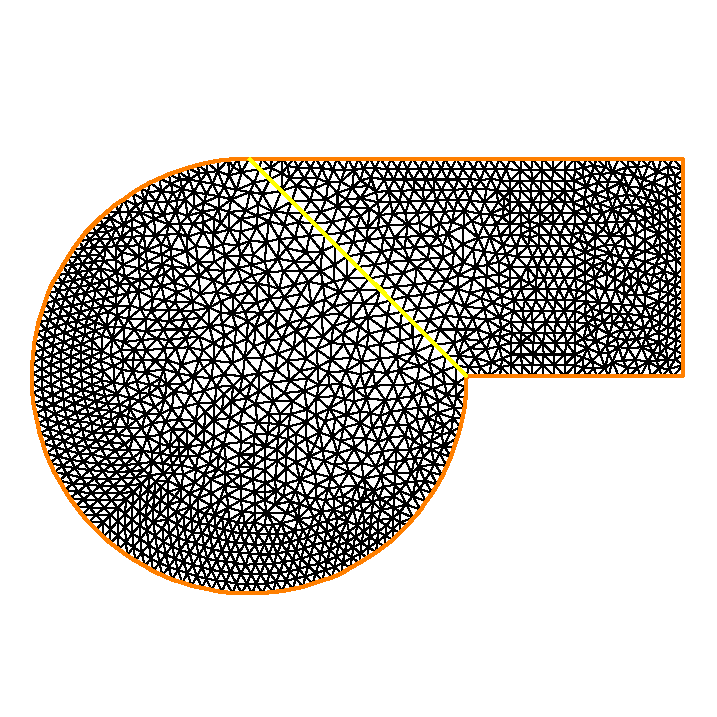
\includegraphics[width=6cm]{schwarz-no-th} \hss}
\caption{ The two none overlapping mesh \texttt{TH} and \texttt{th}  }
\end{figure}

Let introduce  $\Gamma_i$ is  common the boundary of $\Omega_1$ and
$\Omega_2$ and    $\Gamma_e^i= \p \Omega_i \setminus \Gamma_i$.

The problem  find  $\lambda$ such that $ (u_1|_{\Gamma_i}=u_2|_{\Gamma_i}) $
where  $u_i$ is solution of the following Laplace problem:
\eq{
    -\Delta u_i=f\hin\Omega_i\quad
    u_i|_{\Gamma_i}=\lambda \quad
    u_i|_{\Gamma_e^i} = 0
 }

To solve this problem we just make a loop
with upgrading$\lambda$ with
$$\lambda = \lambda {\pm} \frac{(u_1-u_2)}{2}$$
where the sign $+$ or $-$ of ${\pm}$ is choose to have convergence.

\begin{example}[Schwarz-no-overlap.edp]~
\index{tutorial!Schwarz-no-overlap.edp}
\bFF
// schwarz1 without overlapping
@int inside = 2;
@int outside = 1;
@border a(t=1,2){x=t;y=0;label=outside;};
@border b(t=0,1){x=2;y=t;label=outside;};
@border c(t=2,0){x=t ;y=1;label=outside;};
@border d(t=1,0){x = 1-t; y = t;label=inside;};
@border e(t=0, 1){ x= 1-t; y = t;label=inside;};
@border e1(t=pi/2, 2*pi){ x= cos(t); y = sin(t);label=outside;};
@int n=4;
@mesh th = buildmesh( a(5*n) + b(5*n) + c(10*n) + d(5*n));
@mesh TH = buildmesh ( e(5*n) + e1(25*n) );
@plot(th,TH,wait=1,ps="schwarz-no-u.eps");
@fespace vh(th,P1);
@fespace VH(TH,P1);
vh u=0,v; VH U,V;
vh lambda=0;
@int i=0;

@problem PB(U,V,init=i,solver=Cholesky) =
    @int2d(TH)( dx(U)*dx(V)+dy(U)*dy(V) )
  + @int2d(TH)( -V)
  + @int1d(TH,inside)(-lambda*V) +    on(outside,U= 0 ) ;
@problem pb(u,v,init=i,solver=Cholesky) =
    @int2d(th)( dx(u)*dx(v)+dy(u)*dy(v) )
  + @int2d(th)( -v)
  + @int1d(th,inside)(+lambda*v) +    on(outside,u = 0 ) ;


@for ( i=0 ;i< 10; i++)
{
   PB;
   pb;
   lambda = lambda - (u-U)/2;
   @plot(U,u,wait=true);
};

@plot(U,u,ps="schwarz-no-u.eps");

\eFF
\end{example}

\begin{figure}[hbt]
\HLINE{\hss
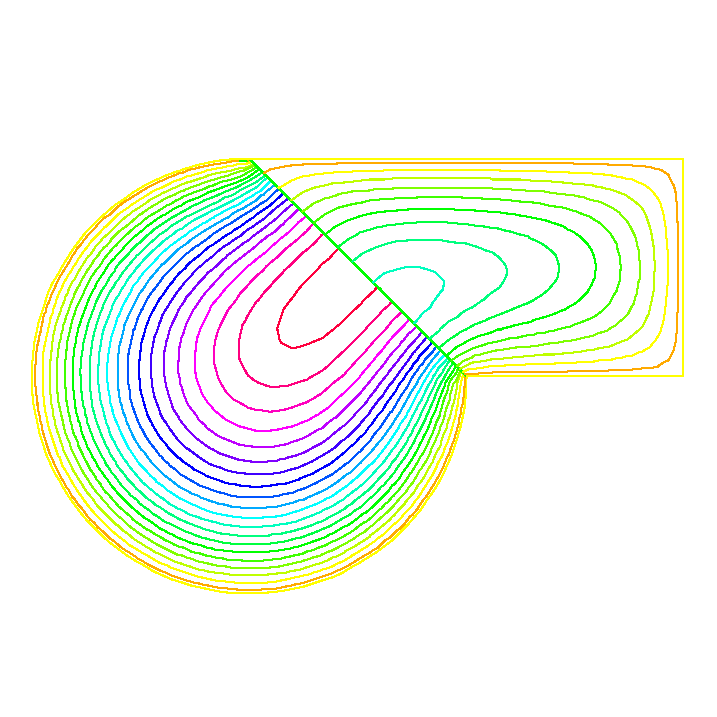
\includegraphics[width=6cm]{schwarz-no-u0}
\hss
\includegraphics[width=6cm]{schwarz-no-u} }
\caption{  Isovalues of the solution at  iteration 0  and iteration 9 without overlapping }
\end{figure}

\subsubsection{Schwarz-gc.edp}
To solve\index{domain decomposition}\index{shurr}
\eq{ -\Delta u =f \hin\Omega=\Omega_1\cup\Omega_2\quad u|_\Gamma=0,}
the Schwarz algorithm for domain decomposition without overlapping  runs like this

Let introduce  $\Gamma_i$ is  common the boundary of $\Omega_1$ and
$\Omega_2$ and    $\Gamma_e^i= \p \Omega_i \setminus  \Gamma_i$.

The problem  find  $\lambda$ such that $ (u_1|_{\Gamma_i}=u_2|_{\Gamma_i}) $
where  $u_i$ is solution of the following Laplace problem:
\eq{
    -\Delta u_i=f\hin\Omega_i\quad
    u_i|_{\Gamma_i}=\lambda \quad
    u_i|_{\Gamma_e^i} = 0
 }

The version of this example for  Shur componant. The border problem
is solve with conjugate gradient.

First, we construct the two domain
\begin{example}[Schwarz-gc.edp]~
\index{tutorial!Schwarz-gc.edp}
\bFF
// Schwarz without overlapping (Shur complenement Neumann -> Dirichet)
@real cpu=clock();
@int inside = 2;
@int outside = 1;

@border Gamma1(t=1,2){x=t;y=0;label=outside;};
@border Gamma2(t=0,1){x=2;y=t;label=outside;};
@border Gamma3(t=2,0){x=t ;y=1;label=outside;};

@border GammaInside(t=1,0){x = 1-t; y = t;label=inside;};

@border GammaArc(t=pi/2, 2*pi){ x= cos(t); y = sin(t);label=outside;};
int n=4;
//  build the mesh of $\Omega_1$ and $\Omega_2$
@mesh Th1 = buildmesh( Gamma1(5*n) + Gamma2(5*n) + GammaInside(5*n) + Gamma3(5*n));
@mesh Th2 = buildmesh ( GammaInside(-5*n) + GammaArc(25*n) );
@plot(Th1,Th2);

// defined the 2 FE space
@fespace Vh1(Th1,P1),      Vh2(Th2,P1);
\eFF
\begin{note}
It is impossible to
define a function just on a part of boundary, so the $\ lambda $
function must be defined on the all domain $\Omega_1$
such as
\bFF
@Vh1 lambda=0;  // take $\lambda \in V_{h1}$
\eFF
\end{note}

The two Poisson problem:
\bFF
@Vh1 u1,v1;              Vh2 u2,v2;
@int i=0;  // for factorization optimization
@problem Pb2(u2,v2,init=i,solver=Cholesky) =
    int2d(Th2)( dx(u2)*dx(v2)+dy(u2)*dy(v2) )
  + int2d(Th2)( -v2)
  + int1d(Th2,inside)(-lambda*v2) +    on(outside,u2= 0 ) ;
@problem Pb1(u1,v1,init=i,solver=Cholesky) =
    int2d(Th1)( dx(u1)*dx(v1)+dy(u1)*dy(v1) )
  + int2d(Th1)( -v1)
  + int1d(Th1,inside)(+lambda*v1) +    on(outside,u1 = 0 ) ;
\eFF
or, we define a border matrix , because the
 $\ lambda $ function is none zero inside the domain $\Omega_1$:
\bFF
@varf b(u2,v2,solver=CG) =int1d(Th1,inside)(u2*v2);
@matrix B= b(Vh1,Vh1,solver=CG);
\eFF

The boundary problem function,
  $$
  \lambda \longrightarrow  \int_{\Gamma_i }(u_1-u_2) v_{1}
$$
\bFF
@func @real[@int] BoundaryProblem(real[int] &l)
{
   lambda[]=l; // make FE function form l
   Pb1;     Pb2;
   i++;  //  no  refactorization i !=0
   v1=-(u1-u2);
   lambda[]=B*v1[];
   @return lambda[] ;
};
\eFF
\begin{note}
The  difference between the two notations \ttCC{v1} and \ttCC{v1[]}  is:
 \ttCC{v1} is the finite element  function and \ttCC{v1[]}
is the vector in the canonical basis of the   finite element  function  \ttCC{v1} .
\index{[]@\verb=[]=}
\end{note}
\bFF
Vh1 p=0,q=0;
//  solve the problem with Conjugate Gradient
LinearCG(BoundaryProblem,p[],eps=1.e-6,nbiter=100);
//  compute the final solution, because CG works with increment
BoundaryProblem(p[]); // solve again  to have right u1,u2

cout << " -- CPU time  schwarz-gc:" <<  clock()-cpu << endl;
plot(u1,u2); // plot
\eFF
\end{example}


%\subsubsection{mortar.edp}
% a faire FH
%  construction de epsi
%  un sous domaine
%  les matrices blocks.


\subsection{Fluid/Structures Coupled Problem}

This problem involves the Lam\'{e} system of elasticity
and the Stokes system for viscous fluids with velocity $\vec u$ and pressure $p$:
\begin{eqnarray*}\Blue
-\Delta \vec u +\vec\nabla p = 0, \,
%\`{u}
\nabla\cdot \vec u = 0,\hbox{~~in ~}\Omega,\,
\vec u=\vec u_\Gamma \hbox{~~on~~}\Gamma=\p\Omega
\end{eqnarray*}\Black
where $u_\Gamma$ is the velocity of the boundaries. The
force  that the fluid applies to the boundaries is the normal stress
\Blue{$$
\vec h =(\nabla\vec u +\nabla\vec u^T)\vec n -p\vec n
$$}

Elastic solids subject to forces deform: a point in the solid,
at (x,y)
goes to (X,Y) after.  When the displacement vector
$\vec v=(v_1,v_2) = (X-x, Y-y)$  is small, Hooke's
law relates the stress tensor $\sigma$ inside the solid to the
deformation tensor $\epsilon$:
\Blue{
 $$ \sigma_{ij} = \lambda \delta_{ij} \nabla.\vec v + 2\mu\epsilon_{ij},
\,
\epsilon_{ij} = {1\over 2}({\p v_i\over\p x_j} +
{\p v_j\over\p x_i} )$$
}
where $\delta$ is the Kronecker symbol
and where $\lambda, \mu$ are two constants describing the material mechanical
properties in terms of the modulus of
elasticity, and Young's modulus.

The equations of elasticity are naturally written in variational form
for the displacement vector $v(x)\in V$ as
\Blue{$$
\int_\Omega [2\mu\epsilon_{ij}(\vec v)\epsilon_{ij}(\vec w)
+\lambda \epsilon_{ii}(v)\epsilon_{jj}(\vec w)]
=\int_\Omega \vec g\cdot \vec w +\int_\Gamma \vec h\cdot \vec w,%\`{u}
\forall \vec w\in V
$$}
The data are the gravity force $\vec g$ and the
boundary stress $\vec h$.

\begin{example}[Fluidstruct.edp]
\index{tutorial!Fluidstruct.edp}
In our example the Lam\'{e} system and the Stokes system are coupled by a
common boundary on which
the fluid  stress creates a displacement of the boundary and hence
changes the shape of the domain where the Stokes problem is integrated.
The geometry is that of a vertical driven cavity with an elastic lid.
The lid is a beam with weight so it will
be deformed by its own weight and by the normal stress due to the fluid reaction.
The cavity is the $10 \times 10$ square and the lid is a rectangle of height $l=2$.
\\\\
A beam sits on a box full of fluid rotating because the left vertical side has velocity one.
The beam is bent by its own weight, but the pressure of the fluid modifies the bending.
\\
The bending displacement of the beam is given by (uu,vv) whose solution is
given as follows.
\bFF
//  Fluid-structure interaction for a weighting beam sitting on a
// square cavity filled with a fluid.

@int bottombeam = 2; // label of bottombeam
@border a(t=2,0)  { x=0; y=t ;label=1;};        //  left beam
@border b(t=0,10) { x=t; y=0 ;label=bottombeam;};        //  bottom of beam
@border c(t=0,2)  { x=10; y=t ;label=1;};       //  rigth beam
@border d(t=0,10) { x=10-t; y=2; label=3;};     //  top beam
@real E = 21.5;
@real sigma = 0.29;
@real mu = E/(2*(1+sigma));
@real lambda = E*sigma/((1+sigma)*(1-2*sigma));
@real gravity = -0.05;
@mesh th = @buildmesh( b(20)+c(5)+d(20)+a(5));
@fespace Vh(th,@P1);
Vh uu,w,vv,s,fluidforce=0;
@cout << "lambda,mu,gravity ="<<lambda<< " " << mu << " " << gravity << @endl;
// deformation of a beam under its own weight
@solve  bb([uu,vv],[w,s])  =
    @int2d(th)(
                 2*mu*(dx(uu)*dx(w)+ ((dx(vv)+dy(uu))*(dx(s)+dy(w)))/4 )
               + lambda*(dx(uu)+dy(vv))*(dx(w)+dy(s))/2
             )
  + @int2d(th) (-gravity*s)
  + @on(1,uu=0,vv=0)
  + fluidforce[];
 ;

 @plot([uu,vv],wait=1);
 @mesh th1 = movemesh(th, [x+uu, y+vv]);
 @plot(th1,wait=1);
\eFF
Then Stokes equation for fluids ast low speed are solved in the box below the beam,
but the beam has deformed the box (see border h):
\bFF
//Stokes on square  b,e,f,g  driven cavite on left side g
@border e(t=0,10) { x=t; y=-10; label= 1; };      //  bottom
@border f(t=0,10) { x=10; y=-10+t ; label= 1; };   //  right
@border g(t=0,10) { x=0; y=-t ;label= 2;};       //  left
@border h(t=0,10) { x=t; y=vv(t,0)*( t>=0.001 )*(t <= 9.999);
                    label=3;};   //  top of cavity deformed

@mesh sh = @buildmesh(h(-20)+f(10)+e(10)+g(10));
@plot(sh,wait=1);
\eFF
 We use the Uzawa conjugate gradient to solve the Stokes problem like in example \refSec{Uzawa}

\bFF
@fespace Xh(sh,P2),Mh(sh,P1);
Xh u1,u2,v1,v2;
Mh p,q,ppp;


@varf bx(u1,q) = @int2d(sh)( -(dx(u1)*q));

@varf by(u1,q) = @int2d(sh)( -(dy(u1)*q));

@varf Lap(u1,u2)= @int2d(sh)(  dx(u1)*dx(u2) + dy(u1)*dy(u2) )
                    +  @on(2,u1=1) +  @on(1,3,u1=0)  ;

Xh bc1; bc1[] = Lap(0,Xh);
Xh brhs;

@matrix A= Lap(Xh,Xh,solver=CG);
@matrix Bx= bx(Xh,Mh);
@matrix By= by(Xh,Mh);
Xh bcx=0,bcy=1;

@func @real[@int] divup(@real[@int] & pp)
{
  @int verb=verbosity;
   verbosity=0;
   brhs[]  = Bx'*pp; brhs[] += bc1[] .*bcx[];
   u1[] = A^-1*brhs[];
   brhs[]  = By'*pp; brhs[] += bc1[] .*bcy[];
   u2[] = A^-1*brhs[];
   ppp[] =   Bx*u1[];
   ppp[] +=  By*u2[];
   verbosity=verb;
   @return ppp[] ;
};

 p=0;q=0;u1=0;v1=0;

 @LinearCG(divup,p[],eps=1.e-3,nbiter=50);
 divup(p[]);
\eFF
Now the beam will feel the stress constraint from the fluid:
\bFF
  Vh sigma11,sigma22,sigma12;
  Vh uu1=uu,vv1=vv;

  sigma11([x+uu,y+vv]) = (2*dx(u1)-p);
  sigma22([x+uu,y+vv]) = (2*dy(u2)-p);
  sigma12([x+uu,y+vv]) = (dx(u1)+dy(u2));
\eFF
which comes as a boundary condition to the PDE of the beam:
\bFF
@varf fluidf([uu,vv],[w,s]) fluidforce =
@solve  bbst([uu,vv],[w,s],init=i)  =
    @int2d(th)(
                 2*mu*(dx(uu)*dx(w)+ ((dx(vv)+dy(uu))*(dx(s)+dy(w)))/4 )
               + lambda*(dx(uu)+dy(vv))*(dx(w)+dy(s))/2
             )
  + @int2d(th) (-gravity*s)
  + @int1d(th,bottombeam)( -coef*(   sigma11*N.x*w + sigma22*N.y*s
                                   + sigma12*(N.y*w+N.x*s) )  )
  + @on(1,uu=0,vv=0);
 @plot([uu,vv],wait=1);
 @real  err = sqrt(@int2d(th)( (uu-uu1)^2 + (vv-vv1)^2 ));
 @cout <<  " Erreur L2 = " << err << "----------\n";
\eFF

Notice that the matrix generated by bbst is reused (see \ttCC{init=i}).
Finally we deform the beam
\bFF
 th1 = @movemesh(th, [x+0.2*uu, y+0.2*vv]);
 @plot(th1,wait=1);
\eFF
\end{example}

\begin{figure}\label{fstruct}
\begin{center}
\includegraphics[width=6.7cm]{fluidstruct1}
\includegraphics[width=6cm,angle=90]{fluidstruct2}
\includegraphics[width=6cm,angle=90]{fluidstruct3}
\caption{ Fluid velocity and pressure (left) and displacement vector (center)
of the structure and displaced geometry (right) in the fluid-structure interaction
of a soft side and a driven cavity}
\end{center}
\end{figure}

\subsection{\setS{Transmission Problem}}
Consider an elastic plate whose displacement change vertically,
which is made up of three plates of different materials,
welded on each other.
Let $\Omega_i,\, i=1,2,3$ be the domain occupied by $i$-th material
with tension $\mu_i$ (see \refSec{Soap Film}).
The computational domain $\Omega$ is the interior of
$\overline{\Omega_1}\cup \overline{\Omega_2}\cup \overline{\Omega_3}$.
The vertical displacement $u(x,y)$ is obtained from
\begin{eqnarray}
\label{eqn:transm-1}
-\mu_i\Delta u&=&f~\textrm{in }\Omega_i\\
\label{eqn:transm-2}
\mu_i\p_n u|_{\Gamma_{i}}&=&-\mu_j\p_n u|_{\Gamma_{j}}
\quad \textrm{on }\overline{\Omega_{i}}\cap\overline{\Omega_{j}}
\qquad \textrm{if }1\le i< j\le 3
\end{eqnarray}
where $\p_n u|_{\Gamma_{i}}$ denotes the value of
the normal derivative $\p_n u$ on the boundary $\Gamma_i$ of
the domain $\Omega_i$.

By introducing the characteristic function $\chi_i$ of $\Omega_i$, that is,
\begin{equation}
\chi_i(x)=1\quad\textrm{if }x\in \Omega_i;\qquad
\chi_i(x)=0\quad\textrm{if }x\not\in \Omega_i
\end{equation}
we can easily rewrite (\ref{eqn:transm-1}) and (\ref{eqn:transm-2})
to the weak form. Here we assume that $u=0$ on $\Gamma=\p\Omega$.

problem Transmission: For a given function $f$, find $u$ such that
\begin{eqnarray}
\label{eqn:transmission}
a(u,v)&=&\ell(f,v)\quad \textrm{for all }v\in H^1_0(\Omega)\\
a(u,v)=\int_{\Omega}\mu \nabla u\cdot \nabla v,\quad
\ell(f,v)=\int_{\Omega}fv\nonumber
\end{eqnarray}
where $\mu=\mu_1\chi_1+\mu_2\chi_2+\mu_3\chi_3$.
Here we notice that $\mu$ become the discontinuous function.

With dissipation, and at the thermal equilibrium, the temperature equation
is:

This example explains the definition and manipulation of \emph{region}, i.e.
\index{subdomains} subdomains of the whole domain.

Consider this L-shaped domain with 3 diagonals as internal boundaries, defining
4 subdomains:

\bFF
//   example using region keyword
// construct a mesh with 4 regions (sub-domains)
border a(t=0,1){x=t;y=0;};
border b(t=0,0.5){x=1;y=t;};
border c(t=0,0.5){x=1-t;y=0.5;};
border d(t=0.5,1){x=0.5;y=t;};
border e(t=0.5,1){x=1-t;y=1;};
border f(t=0,1){x=0;y=1-t;};
//  internal boundary
border i1(t=0,0.5){x=t;y=1-t;};
border i2(t=0,0.5){x=t;y=t;};
border i3(t=0,0.5){x=1-t;y=t;};

mesh th = buildmesh (a(6) + b(4) + c(4) +d(4) + e(4) +
    f(6)+i1(6)+i2(6)+i3(6));
fespace Ph(th,P0);  // constant discontinuous functions / element
fespace Vh(th,P1);  // $P_1$ continuous functions / element

Ph reg=region; //  defined the $P_0$ function  associated to region number
plot(reg,fill=1,wait=1,value=1);
\eFF
\twoplot[height=8cm]{region}{region_nu}{the function \texttt{reg}}{the function \texttt{nu} }

\index{region} \texttt{region}  is a keyword of freefem++ which is in fact a variable depending of
the current position (is not a function today, use \texttt{Ph reg=region;} to  set  a function).  This variable value returned is the number of the
subdomain of the current position.  This number is defined by "buildmesh" which scans while building the mesh all
its connected component.  So to get the number of a region containing a particular point
one does:
\bFF

int nupper=reg(0.4,0.9); // get the region number of point (0.4,0.9)
int nlower=reg(0.9,0.1);  // get the region number of point (0.4,0.1)
cout << " nlower " <<  nlower << ", nupper = " << nupper<< endl;
//  defined the characteristics functions of upper and lower region
Ph nu=1+5*(region==nlower) + 10*(region==nupper);
plot(nu,fill=1,wait=1);
\eFF
This is particularly useful to define \index{discontinuous functions}discontinuous functions such as might occur
when one part of the domain is copper and the other one is iron, for example.
\\
We this in mind we proceed to solve a Laplace equation with discontinuous coefficients
($\nu$ is 1, 6 and 11 below).
\bFF
Ph nu=1+5*(region==nlower) + 10*(region==nupper);
plot(nu,fill=1,wait=1);
problem lap(u,v) =   int2d(th)( nu*( dx(u)*dx(v)*dy(u)*dy(v) ))
                   + int2d(-1*v) + on(a,b,c,d,e,f,u=0);
plot(u);
\eFF
\plot[height=8cm]{region_u}{the isovalue of the solution $u$}
\newpage

\subsection{Free Boundary Problem}

The domain $\Omega$ is defined with:

\bFF
@real L=10;        //longueur du domaine
@real h=2.1;      // hauteur du bord gauche
@real h1=0.35;    // hauteur du bord droite

//  maillage d'un tapeze
@border a(t=0,L){x=t;y=0;};       // bottom:  $\Gamma_a$ \hfill
@border b(t=0,h1){x=L;y=t;};      // right:  $\Gamma_b$ \hfill
@border f(t=L,0){x=t;y=t*(h1-h)/L+h;}; //  free surface:  $\Gamma_f$ \hfill
@border d(t=h,0){x=0;y=t;};      // left:  $\Gamma_d$ \hfill

@int n=4;
@mesh Th=@buildmesh (a(10*n)+b(6*n)+f(8*n)+d(3*n));
@plot(Th,ps="dTh.eps");
\eFF


\begin{figure}[hbt]
\includegraphics[width=15cm]{dTh}
\caption{The mesh of the domain $\Omega$}
\end{figure}

The free boundary problem is:

Find $u$ and $\Omega$ such that:

 $$ \left\{\begin{array}{cl}
 \displaystyle - \Delta u = 0  & \mbox{in } \Omega\\
 \displaystyle      u = y         &\mbox{on } \Gamma_b \\
 \displaystyle      {\p u  \over \p n} = 0   &\mbox{on } \Gamma_d \cup \Gamma_a \\
 \displaystyle    {\p u  \over \p n} = { q\over K} n_x
          \mbox{\ and \ } {u = y}  &\mbox{on\ } \Gamma_ f
\end{array}\right. $$


We use a fixed point method;
$\Omega^0 = \Omega$

in two step, fist we solve the classical following problem:
$$ \left\{\begin{array}{rll}
 \displaystyle - \Delta u &= 0  & \mbox{in } \Omega^n\\
 \displaystyle      u &= y         &\mbox{on } \Gamma^n_b \\
 \displaystyle      {\p u  \over \p n} &= 0   &\mbox{on } \Gamma^n_d \cup \Gamma^n_a\\
 \displaystyle    u &= y        &\mbox{on\ } \Gamma^n_ f
\end{array}\right. $$

The variational formulation is:

find $u$ on $V=H^1(\Omega^n)$, such than  $u=y$ on $\Gamma^n_b$ and $\Gamma^n_f$
$$
 \int_{\Omega^n}  \nabla u \nabla u' = 0,  \quad \forall u' \in V  \mbox{ with }  u' =0 \mbox{ on }
\Gamma^n_b \cup \Gamma^n_f
$$


and secondly to construct a domain deformation $\mathcal{F}(x,y)=[x,y-v(x,y)]$

where $v$ is  solution of  the following problem:

 $$ \left\{\begin{array}{rll}
 \displaystyle - \Delta v &= 0  & \mbox{in } \Omega^n\\
 \displaystyle      v  &= 0         &\mbox{on } \Gamma^n_a \\
 \displaystyle      {\p v \over \p n} &= 0   &\mbox{on } \Gamma^n_b \cup \Gamma^n_d \\
 \displaystyle    {\p v  \over \p n}  &=  \displaystyle {\p u  \over \p n} - { q\over K} n_x
            &\mbox{on\ } \Gamma^n_ f
\end{array}\right. $$

The variational formulation is:

find $v$ on $V$, such than  $v=0$ on $\Gamma^n_a$
$$
 \int_{\Omega^n}  \nabla v \nabla v' = \int_{\Gamma_f^n}  ({\p u  \over \p n} - { q\over K} n_x )v',  \quad \forall v' \in V  \mbox{ with }  v' =0 \mbox{ on }
\Gamma^n_a
$$

Finally the new domain
$\Omega^{n+1} = \mathcal{F}(\Omega^n)$



\begin{example}[freeboundary.edp]
\index{tutorial!freeboundary.edp}
The  \texttt{FreeFem++} :implementation is:

\bFF
@real q=0.02;      //flux entrant
@real K=0.5;           //permeabilit\'{e}

@fespace Vh(Th,P1);
@int j=0;

Vh u,v,uu,vv;

@problem Pu(u,uu,solver=CG) = @int2d(Th)( dx(u)*dx(uu)+dy(u)*dy(uu))
  + @on(b,f,u=y) ;

@problem Pv(v,vv,solver=CG) = @int2d(Th)( dx(v)*dx(vv)+dy(v)*dy(vv))
  +  @on (a, v=0) + @int1d(Th,f)(vv*((q/K)*N.y- (dx(u)*N.x+dy(u)*N.y)));


@real errv=1;
@real erradap=0.001;
verbosity=1;
@while(errv>1e-6)
{
  j++;
  Pu;
  Pv;
  @plot(Th,u,v ,wait=0);
  errv=int1d(Th,f)(v*v);
   real coef=1;

//
  real mintcc = @checkmovemesh(Th,[x,y])/5.;
  real mint = @checkmovemesh(Th,[x,y-v*coef]);

  if (mint<mintcc ||  j%10==0) {  // mesh to bad => remeshing
    Th=@adaptmesh(Th,u,err=erradap ) ;
    mintcc = @checkmovemesh(Th,[x,y])/5.;
  }

  @while (1)
  {
    real mint = @checkmovemesh(Th,[x,y-v*coef]);

    if (mint>mintcc) break;

    cout << " min |T]  " << mint << endl;
    coef /= 1.5;
  }

  Th=@movemesh(Th,[x,y-coef*v]); // calcul de la deformation
  cout << "\n\n"<<j <<"------------ errv = " << errv << "\n\n";

}
@plot(Th,ps="d_Thf.eps");
@plot(u,wait=1,ps="d_u.eps");
\eFF
\end{example}

\begin{figure}[hbt]
\includegraphics[width=15cm]{d_u}
\caption{The final solution on  the new  domain $\Omega^{72}$}
\end{figure}
\begin{figure}[hbt]
\includegraphics[width=15cm]{d_Thf}
\caption{The adapted mesh of the domain $\Omega^{72}$}
\end{figure}

\textBlack\subsection{nolinear-elas.edp}
\textBlack
The nonlinear elasticity  problem is find  the displacement $(u_{1},u_{2})$  minimizing  $J$
$$ \min J(u_{1},u_{2}) = \int_{\Omega} f(F2) -  \int_{\Gamma_{p}} P_{a} \,  u_{2} $$
where  $F2(u_{1},u_{2}) =  A(E[u_{1},u_{2}],E[u_{1},u_{2}])$ and $A(X,Y)$ is bilinear sym. positive form with respect two matrix $X,Y$.
where $f$ is a given $\mathcal{C}^2$  function, and $E[u_{1},u_{2}] = (E_{ij})_{i=1,2,\,j=1,2}$ is the Green-Saint Venant deformation tensor defined  with:
$$  E_{ij} = 0.5 ( \p_i u_j + \p_j u_i ) + \sum_k \p_i u_k {\times} \p_j u_k  $$



The differential of $J$ is
  $$ DJ(u_{1},u_{2})(v_{1},v_{2}) = \int 2 A(E[u_{1},u_{2}],DE[u_{1},u_{2}](v_{1},v_{2})) f'(F2(u_{1},u_{2}))) -  \int_{\Gamma_{p}} P_{a}  u_{2}  $$

denote $\mathbf{u}=u_{1},u_{2}$, $\mathbf{v}=v_{1},v_{2}$, $\mathbf{w}=(w_{1},w_{2})$ and
the second order differential is
 {\begin{eqnarray*}
 D^2 J(\mathbf{u})((\mathbf{v}),(\mathbf{w}))  &= & A(E[\mathbf{u}],DE[\mathbf{u}](\mathbf{v})) A(E[\mathbf{u}],DE[\mathbf{u}](\mathbf{w})) f''(F2(\mathbf{u}))) \\
 & + &  A(DE[\mathbf{u}](\mathbf{v}),DE[\mathbf{u}](\mathbf{w})) f'(F2(\mathbf{u}))) \\
 &+&  A(DE[\mathbf{u}],D^{2}E[\mathbf{u}]((\mathbf{v}),(\mathbf{w}))) f'(F2(\mathbf{u})))
\end{eqnarray*}}
 where $DE$ and $D^{2}E$ are the first and second differential of $E$.

 \medskip


The Newton Method is

choose $ n=0$,and $u_O,v_O$ the initial displacement
\begin{itemize}
\item loop: \\
\item  \hspace{1cm}    find $(du,dv)$ :  solution of
$$ D^2J(u_n,v_n)((w,s),(du,dv)) =  DJ(u_n,v_n)(w,s) , \quad \forall w,s $$
\item  \hspace{1cm}      $un =un - du,\quad vn =vn - dv$
\item  \hspace{1cm}      until $(du,dv)$ small is enough
\end{itemize}

\color{black}The way to implement this algorithm in \freefempp is
use a macro tool to implement  $A$ and $F2$, $f$, $f'$,$f''$.

A macro\label{macro}\index{macro} is like is \texttt{ccp} preprocessor of \Cpp, but this begin by
\texttt{macro} and the end of the macro definition is the begin of the comment $//$.
In this case the macro is very useful because the type of parameter can be change.
And  it is easy to make automatic differentiation.
\begin{figure}[hbt]
\begin{center}\includegraphics[width=10cm]{nl-elas}\end{center}
\caption{\label{fig nl-elas} The deformated domain}
\end{figure}

\bFF
//  non linear elasticity model \hfilll
//   \hfilll
//  -------------------------------\hfilll
//  with huge utilization of  macro\hfilll
// ---------------------------\hfilll
//   optimize version \hfilll
// ------------\hfilll
//  @problem is  find $(uu,vn)$  minimizing  $J$\hfilll
//  $ min J(un,vn) = @int f(F2) -  @int Pa * un $\hfilll
//   $ dJ(u,u,uu,vv) = @int dF2(u,v,uu,vv) df(F2(u,v))$ \hfilll
//   where $F2 =  (^t {E}  A {E} )$ , \hfilll
//   $E(U) =  1/2 (\nabla U + \nabla U^t + \nabla U^t  \nabla U) $ \hfilll
//         ($u_1$) \hfilll
//  with U=(   )\hfilll
//         ($u_2$)\hfilll
// so: \hfilll
// \hfilll$$ E_{ij} = 0.5 ( d_i u_j + d_j u_i ) + \sum_k d_i u_k * d_j*u_k  \leqno(1)$$
//  the 3 components of the Green Saint-Venant deformation tensor: \hfilll
//  $E1(u1,u2) =    E_{11} $\hfilll
//  $E2(u1,u2) =    E_{12} = E_21 $\hfilll
//  $E3(u1,u2) =    E_{22}  $\textBlack\hfilll
\eFF
~
\bFF
// remark : we can parametrize E1,E2,E3 with:\hfilll
//  EE(da,db,a,b,u1,u2) \hfilll
//   where $da,db$ correspond to $d_i, d_j$ in (1)\hfilll
//   where  $a,b$  correspond to $u_i, u_j$ in (1)\hfilll
//   where $u1,u2$  correspond to $u_1, u_2$ in (1)\hfilll
//  ----------------------------------------------

//  first the linear part of EE linear elasticite\hfilll
// remark a macro end with a // comment \hfilll
@macro EEL(di,dj,ui,uj) ( (di(uj)+dj(ui))*0.5 )    // 11

// non linear par of EE (bilinear)  simple to differential \hfilll
@macro bEENL(di,dj,u1,u2,v1,v2) (di(u1)*dj(v1)*.5+di(u2)*dj(v2)*0.5)
//
@macro EENL(di,dj,u1,u2) bEENL(di,dj,u1,u2,u1,u2) //
@macro dEENL(di,dj,u1,u2,du1,du2) ( bEENL(di,dj,du1,du2,u1,u2)
                                  + bEENL(di,dj,u1,u2,du1,du2) )
//   ------------ \hfilll
@macro EE(di,dj,ui,uj,u1,u2) (EEL(di,dj,u1,uj) + EENL(di,dj,u1,u2)) //
@macro dEE(di,dj,dui,duj,u1,u2,du1,du2) (EEL(di,dj,du1,duj)
                                         + dEENL(di,dj,u1,u2,du1,du2)) //
@macro ddEE(di,dj,du1,du2,ddu1,ddu2) ( dEENL(di,dj,du1,du2,ddu1,ddu2))
//
// remark  : \hfilll
// $ dEE(di,dj,dui,duj,u1,u2,du1,du2)$  is "the formal differential of EE" \hfilll
// where $du1=\delta u1$ ,$du2=\delta u2$ \hfilll
// $ ddEE(di,dj,dui,duj,u1,u2,du1,du2)$  is "the formal differential of dEE" \hfilll
// where $ddu1=\delta^2 u1$ ,$ddu2=\delta^2 u2$ \hfilll
// --- \hfilll

//  the macro corresponding to the 3 componante of E \hfilll
@macro E1(u,v)  /*E11*/EE(dx,dx,u,u,u,v)  //
@macro E2(u,v)  /*E12*/EE(dx,dy,u,v,u,v)  //
@macro E3(u,v)  /*E22*/EE(dy,dy,v,v,u,v)  //

@macro dE1(u,v,uu,vv) /*dE11*/dEE(dx,dx,uu,uu,u,v,uu,vv) //
@macro dE2(u,v,uu,vv) /*dE12*/dEE(dx,dy,uu,vv,u,v,uu,vv) //
@macro dE3(u,v,uu,vv) /*dE22*/dEE(dy,dy,vv,vv,u,v,uu,vv) //
@macro ddE1(u,v,uu,vv,uuu,vvv) /*ddE11*/ddEE(dx,dx,uu,vv,uuu,vvv) //
@macro ddE2(u,v,uu,vv,uuu,vvv) /*ddE12*/ddEE(dx,dy,uu,vv,uuu,vvv) //
@macro ddE3(u,v,uu,vv,uuu,vvv) /*ddE22*/ddEE(dy,dy,uu,vv,uuu,vvv)
//
//  a formal bilinear term \hfilll
@macro PP(A,B,u,v) (A(u,v)*B(u,v))
//
// a formal diff  bilinear term \hfilll
@macro dPP(A,B,dA,dB,u,v,uu,vv) (dA(u,v,uu,vv)*B(u,v) + A(u,v)*dB(u,v,uu,vv))
//
// a formal $diff^2$ bilinear term \hfilll
@macro ddPP(A,B,dA,dB,ddA,ddB,u,v,uu,vv,uuu,vvv) (
  dA(u,v,uu,vv)*dB(u,v,uuu,vvv) + dA(u,v,uuu,vvv)*dB(u,v,uu,vv)
  +  ddA(u,v,uu,vv,uuu,vvv)*B(u,v) + A(u,v)*ddB(u,v,uu,vv,uuu,vvv)
  ) //
// so the @matrix A is 6 coef \hfilll
//
//     a11 a12 a13 \hfilll
//     a12 a22 a23 \hfilll
//     a13 a23 a33 \hfilll
@macro F2(u,v)  /* F2 */  (
     a11*PP(E1,E1,u,v)
  +  a22*PP(E2,E2,u,v)
  +  a33*PP(E3,E3,u,v)
  +  a13*PP(E1,E3,u,v)
  +  a13*PP(E3,E1,u,v)
  +  a12*PP(E1,E2,u,v)
  +  a12*PP(E2,E1,u,v)
  +  a23*PP(E2,E3,u,v)
  +  a23*PP(E3,E2,u,v)
)  // end macro F2

@macro dF2(u,v,uu,vv)  /* dF2 */  (
       a11*dPP(E1,E1,dE1,dE1,u,v,uu,vv)
     + a12*dPP(E1,E2,dE1,dE2,u,v,uu,vv)
     + a13*dPP(E1,E3,dE1,dE3,u,v,uu,vv)
     + a21*dPP(E2,E1,dE2,dE1,u,v,uu,vv)
     + a22*dPP(E2,E2,dE2,dE2,u,v,uu,vv)
     + a23*dPP(E2,E3,dE2,dE3,u,v,uu,vv)
     + a31*dPP(E3,E1,dE3,dE1,u,v,uu,vv)
     + a32*dPP(E3,E2,dE3,dE2,u,v,uu,vv)
     + a33*dPP(E3,E3,dE3,dE3,u,v,uu,vv)
) // end macro dF2 ($D F2$)

@macro ddF2(u,v,uu,vv,uuu,vvv)  /* ddF2 */  (
       a11*ddPP(E1,E1,dE1,dE1,ddE1,ddE1,u,v,uu,vv,uuu,vvv)
     + a12*ddPP(E1,E2,dE1,dE2,ddE1,ddE2,u,v,uu,vv,uuu,vvv)
     + a13*ddPP(E1,E3,dE1,dE3,ddE1,ddE3,u,v,uu,vv,uuu,vvv)
     + a21*ddPP(E2,E1,dE2,dE1,ddE2,ddE1,u,v,uu,vv,uuu,vvv)
     + a22*ddPP(E2,E2,dE2,dE2,ddE2,ddE2,u,v,uu,vv,uuu,vvv)
     + a23*ddPP(E2,E3,dE2,dE3,ddE2,ddE3,u,v,uu,vv,uuu,vvv)
     + a31*ddPP(E3,E1,dE3,dE1,ddE3,ddE1,u,v,uu,vv,uuu,vvv)
     + a32*ddPP(E3,E2,dE3,dE2,ddE3,ddE2,u,v,uu,vv,uuu,vvv)
     + a33*ddPP(E3,E3,dE3,dE3,ddE3,ddE3,u,v,uu,vv,uuu,vvv)
) // end macro ddF2  ($D^{2}  F2$)

//  differential of J: \hfilll

//  @for hyper elasticity @problem  \hfilll
//  ------------------------------ \hfilll

@macro f(u) (u) // end of macro
@macro df(u) (1) // end of macro  $df=f'$
@macro ddf(u) (0) // end of macro $ddf=f''$

//  -- du caoutchouc --- CF cours de Herve Le Dret. \hfilll
// ------------------------------- \hfilll
@real mu = 0.012e5; //  $kg/cm^2$
@real lambda =  0.4e5; //  $kg/cm^2$
//  \hfilll
//   $  \sigma = 2 \mu E + \lambda tr(E) Id $  \hfilll
//    \hfilll
//   ( a b )  \hfilll
//   ( b c )  \hfilll
//  \hfilll
//  tr*Id : (a,b,c) -> (a+c,0,a+c)  \hfilll
// so the associed @matrix is:  \hfilll
//   ( 1 0 1 )  \hfilll
//   ( 0 0 0 )  \hfilll
//   ( 1 0 1 )  \hfilll
// ------------------ the coef \hfilll
@real a11= 2*mu +  lambda  ;
@real a22= 2*mu ;
@real a33= 2*mu +   lambda ;
@real a12= 0 ;
@real a13= lambda ;
@real a23= 0 ;
//  symetric part
@real a21= a12 ;
@real a31= a13 ;
@real a32= a23 ;
@real Pa=1e2; //  a pressure of 100 Pa
// ----------------

@int n=30,m=10;
@mesh Th= square(n,m,[x,.3*y]); // label: 1 bottom, 2 right, 3 up, 4 left;
@int bottom=1, right=2,upper=3,left=4;

@plot(Th);

@fespace Wh(Th,P1dc);
@fespace Vh(Th,[P1,P1]);
@fespace Sh(Th,P1);

Wh e2,fe2,dfe2,ddfe2; // optimisation
Wh ett,ezz,err,erz; // optimisation

Vh [uu,vv], [w,s],[un,vn];
[un,vn]=[0,0];//  intialisation
[uu,vv]=[0,0];

@varf vmass([uu,vv],[w,s],solver=CG) =  @int2d(Th)( uu*w + vv*s );
@matrix M=vmass(Vh,Vh);

@problem NonLin([uu,vv],[w,s],solver=LU)=
 @int2d(Th,qforder=1)( // $(D^2 J(un))$ part
               ddF2(un,vn,uu,vv,w,s)* dfe2
       + dF2(un,vn,uu,vv)*dF2(un,vn,w,s)*ddfe2
        )
   -@int2d(Th,<1)( // $(D J(un))$ part
           dF2(un,vn,w,s) * dfe2  )
   - @int1d(Th,3)(Pa*s)
   + @on(right,left,uu=0,vv=0);
;
// Newton's method
// ---------------
Sh u1,v1;
@for (@int i=0;i<10;i++)
{
  @cout << "Loop " << i << @endl;
  e2 = F2(un,vn);
  dfe2 = df(e2) ;
  ddfe2 = ddf(e2);
  @cout << "  e2 max " <<e2[].max << " , min" << e2[].min << @endl;
  @cout << " de2 max "<< dfe2[].max << " , min" << dfe2[].min << @endl;
  @cout << "dde2 max "<< ddfe2[].max << " , min" << ddfe2[].min << @endl;
  NonLin; //  compute $[uu,vv] = (D^2 J(un))^{-1}(D J(un))$

  w[]   = M*uu[];
  @real res = sqrt(w[]' * uu[]); //  norme $ L^2 of [uu,vv]$
  u1 = uu;
  v1 = vv;
  @cout << " L^2 residual = " << res << @endl;
  @cout << " u1 min =" <<u1[].min << ", u1 max= " << u1[].max << @endl;
  @cout << " v1 min =" <<v1[].min << ", v2 max= " << v1[].max << @endl;
  @plot([uu,vv],wait=1,cmm=" uu, vv " );
  un[] -= uu[];
  @plot([un,vn],wait=1,cmm=" deplacement " );
  @if (res<1e-5) @break;
}

@plot([un,vn],wait=1);
@mesh th1 = @movemesh(Th, [x+un, y+vn]);
@plot(th1,wait=1); //  see figure \ref{fig nl-elas}
\eFF




\section{Parallel version experimental}
A first attempt of parallelization of \texttt{FreeFem++} is made here with {\bf\texttt{mpi}}.
We add 4 words in the language:
\begin{description}
\itemtt[mpisize] The total number of  processes\index{mpisize}
\itemtt[mpirank]  the number of my current process in $\{0,..., mpisize-1\}$.\index{mpirank}
\itemtt [processor] a function to set the possessor to send or receive data
\itemtt [broadcast] a function to broadcast from a processor to all other a data \index{broadcast}\index{processor}
\bFF
    processor(10) << a ; // send to the process 10 the data a;
    processor(10) >> a ; // receive from the process 10 the data a;

\eFF
\end{description}
\subsection{Schwarz in parallel}
This example is just the rewritting of example \texttt{schwarz-overlap}
in section \ref{schwarz-overlap}.\index{schwarz}\index{broadcast}\index{processor}
\index{array!mesh}

\bFF
[examples++-mpi] Hecht%lamboot

LAM 6.5.9/MPI 2 C++/ROMIO - Indiana University


[examples++-mpi] hecht% mpirun -np 2 FreeFem++-mpi schwarz-c.edp
\eFF

\bFF
//  a new coding version c,   methode de schwarz in parallele \hfilll
// with 2 proc. \hfilll
//  ------------------------------- \hfilll
// F.Hecht december 2003 \hfilll
// ---------------------------------- \hfilll
//  to test the broadcast instruction \hfilll
//  and array of mesh  \hfilll
//  add add the stop test \hfilll
//  --------------------------------- \hfilll

@if ( mpisize != 2 ) {
  @cout << " sorry number of processeur !=2 " << endl;
  exit(1);}
@verbosity=3;
@real pi=4*atan(1);
@int inside = 2;
@int outside = 1;
@border a(t=1,2){x=t;y=0;label=outside;};
@border b(t=0,1){x=2;y=t;label=outside;};
@border c(t=2,0){x=t ;y=1;label=outside;};
@border d(t=1,0){x = 1-t; y = t;label=inside;};
@border e(t=0, pi/2){ x= cos(t); y = sin(t);label=inside;};
@border e1(t=pi/2, 2*pi){ x= cos(t); y = sin(t);label=outside;};
@int n=4;
@mesh[int]  Th(mpisize);
@if (mpirank == 0)
 Th[0] = buildmesh( a(5*n) + b(5*n) + c(10*n) + d(5*n));
@else
 Th[1] = buildmesh ( e(5*n) + e1(25*n) );

@broadcast(@processor(0),Th[0]);
@broadcast(@processor(1),Th[1]);

@fespace Vh(Th[mpirank],P1);
@fespace Vhother(Th[1-mpirank],P1);

Vh u=0,v;
Vhother U=0;
@int i=0;

@problem pb(u,v,init=i,solver=Cholesky) =
    @int2d(Th[mpirank])( dx(u)*dx(v)+dy(u)*dy(v) )
  - @int2d(Th[mpirank])( v)
  + @on(inside,u = U)  +  @on(outside,u= U ) ;

@for ( i=0 ;i< 20; i++)
{
  @cout << mpirank << " looP " << i << endl;
   pb;
   //  send u  to the other proc, receive in U
   @processor(1-mpirank) << u[];   @processor(1-mpirank) >> U[];
   @real err0,err1;
   err0 = int1d(Th[mpirank],inside)(square(U-u)) ;
   // send err0  to the other proc, receive in err1
   @processor(1-mpirank)<<err0;   @processor(1-mpirank)>>err1;
   @real err= sqrt(err0+err1);
   @cout <<" err = " << err << " err0 = " << err0
         << ", err1 = " << err1 << endl;
   @if(err<1e-3) @break;
};
@if (mpirank==0)
    @plot(u,U,ps="uU.eps");

\eFF



\section{Graphical User Interface}

There are two different graphical user interfaces available for
\freefempp:

\begin{itemize}
\item \texttt{FreeFem++-cs} is part of the standard \freefempp
package. It runs on Linux, MacOS X and Windows.
\item \texttt{FFedit} is available as a separate package. It runs on
Linux and MacOS~X and requires tcl/tk to be installed.
\end{itemize}

\subsection{FreeFem++-cs}

``-cs'' stands for ``client/server''. The executable program named
\texttt{FreeFem++-cs} is the client. It automatically starts a server
program named \texttt{FreeFem++-cs-server} every time the user asks
for a script to be run. To run \texttt{FreeFem++-cs}, just type its
name in, optionally followed by a script name. It will open a window
corresponding to fig. \ref{fig:FreeFem++-cs}.

\begin{figure}[htbp]
\begin{center}
  \includegraphics[height=10cm]{figures/FreeFem++-cs}
\end{center}
  \caption{\texttt{FreeFem++-cs} main window}
  \label{fig:FreeFem++-cs} \index{label}
\end{figure}

\bigskip

The main characteristics of \texttt{FreeFem++-cs} are~:

\begin{itemize}
\item A main window composed of three panels~: editor with syntax
highlighting (right), \freefempp messages (bottom) and graphics
(left).
\item Panel sizes can be changed. Any of the three panels can be made
to fill the whole window.
\item The edited script can be run at any time by clicking on the
``Run'' button.
\item Graphics can be examined (e.g. zoomed) while \freefempp is
running.
\item A running \freefempp computation can be paused or stopped at any
time.
\end{itemize}

\bigskip

All commands should be self-explanatory. Here are just a few
useful hints~:

\begin{itemize}
\item There is no need to save a \freefempp script to run it. It is
run exactly as displayed in the editor window, and the corresponding
file is not touched.
\item The current directory is updated every time a script is loaded
or saved. All \texttt{include} directives are therefore relative to
the directory where the main script is located.
\item Specifying \texttt{wait=1} in a \texttt{plot} command is exactly
equivalent to clicking on the ``Pause'' button when the plot is
displayed.
\end{itemize}

\subsection{FFedit}

FFedit runs on Linux and MacOSX.\\

\subsubsection{Installation of Tcl and Tk}

You have to install tcl8.4.6 and tk8.4.6 for the GUI to work.\\
First go to http:\\
//www.tcl.tk./software/tcltk/downloadnow84.tml \\
and download :\\
tcl8.4.6-src.tar.gz and tk8.4.6-src.tar.gz\\
Then do :\\
tar zxvf tcl8.4.6-src.tar.gz\\
tar zxvf tk8.4.6-src.tar.gz\\
It creates two directories : tcl8.4.6 and tk8.4.6\\
Now do : \\
cd tcl8.4.6\\
cd unix (if your OS is Linux or MacOSX)\\
./configure\\
make\\
make install\\
\\
then \\
cd tk8.4.6\\
cd unix\\
./configure\\
make\\
make install\\
\\
At the end of installation, you have to find where is your binary ``wish'' or ``wish84'' or ``wish8.4'' by typing :\\
-$>$ which wish (or wish84 or wish8.4)\\
If wish84 does exist it is all. If not, you have to go in the directory where is ``wish'' or ``wish8.4'' (for example /usr/bin/)\\
and then create a link :\\
-$>$ ln -s wish wish84\\
or\\
-$>$ ln -s wish8.4 wish84\\

\subsubsection{Description}

The Graphic User Interface is in the directory called FFedit.
You can run it by typing ./FFedit.tcl\\
\
The Graphic User Interface shows a text window with buttons on the left and right side, a horizontal menu bar above and an entry below where you can see the path of the script when it is opened or where you can type the path of a script to run it.\\
\\
This is the description of the different functions of the GUI :\\
\\
*New : you can access it by the button ``New'' on the right side or by selecting it in the menu File on the horizontal bar.\
It deletes the current script and enables you to type a new script.\\
\\
*Open : you can access it by the button ``Open'' on the right side or by selecting it in the menu File or by typing simultaneously ctrl+o on the keyboard.\
It enables you to select a script which has been saved. This script is then opened in the text window. Then, you can modify it, save the changes, save under another name or run it.\\
\\
*Save : you can access it by the button ``Save'' on the right side or by selecting it in the menu File or by typing simultaneously ctrl+s on the keyboard.\
It enables you to save the changes of a script.\\
\\
*Save as : you can access it by the button ``Save As'' on the right side or by selecting it in the menu File.\\
It enables you to locate where you want to save your script and to choose your the name of your script.\\
\\
*Run : you can access it by the button ``Run'' on the right side or by selecting it in the menu File or by typing simultaneously ctrl+r on the keyboard.\\
It enables you to run the current script.\\
Warning: when you run by typing ctrl+r, the cursor must be in the text window.\\
\\
*Print : you can access it by the button ``Print'' on the right side or by selecting it in the menu File or by typing simultaneously ctrl+p on the keyboard.\\
It enables you to print your script. You have to choose the name of the printer.\\
\\
*Help (under construction) : you can access it by the button ``Help'' on the left side. When an example is opened, it shows you a documentation about this example.\\
Warning : The bottom of each page is not accessible, you have to print to see the entire document.\\
\\
*Example : you can access it by the button ``Ex'' on the left side.\
It runs a little example.\\
\\
*Read Mesh : you can access it by the button ``R.M'' on the left side.\
It enables you to read a mesh which has been saved. It adds the command in your script so that you can use it in your script.\\
\\
*Polygonal Border : you can access it by the button ``P.B'' on the left side.\\
It enables you to build a polygonal border.\\
When you click on this button, a new window is opened : you have to click on the button ``Border'' then it asks you how many borders you want. When you enter a number and click on ``OK'' the exact number of couple of entries enable you to enter the coordinates of the vertices. And then you have to enter the number of points on each border. The border number 1 is the segment between the vertex number 1 and the vertex number 2 ...etc...\\
You must turn in the opposite sens of needles of a watch.\\
When you have finished, you have to click on the button ``Build''. It builds the domain with polygonal border and shows the result.\\
Then you can save the result by clicking on the button ``S.Mesh''. Choose the extension .msh for the name.\\
\\
*Navier Stokes : you can access it by the button ``N.S'' on the left side.\\
A new window is opened. You have to build your polygonal domain by clicking on the button ``Border'' it works like the Polygonal Border function.\\
You can save by clicking on the button ``S.Mesh''. Choose the extension .msh for the name.\\
Then you have to choose the Limits Condition by clicking on the buton ``L.C''.\\
First choose between ``Free'' or ``Imposed', then click on the button ``Validate'' and enter the expression of Imposed condition. You have to enter the tangential and the normal component of the velocity. Then click on ``Validate'' again.\\
The expression of the limit condition can be a number but a mathematical expression as well.\\
\\
*emc2 : you can access it by the button ``emc2''. It runs emc2 the mesh building software \\
(http://www-rocq1.inria.fr/gamma/cdrom/\\
www/emc2/fra.htm)\\
\\
*Set up : you can access it by the button ``set up''. It is the first thing you have to do when you use FFedit for the first time.\\
When you click on this button, a new window is opened, with two entries where you have to enter the path of the binary of FreeFem++ (where you compiled or installed) and the path of the scripts (programs written with FreeFem++) for instance the examples provided in FreeFem++.\\
\\
*Undo : you can access it by selecting in the menu Edit or by typing simultaneously ctrl+z. It is an unlimited undo function.\\
\\
*Redo : you can access it by selecting in the menu Edit or by typing simultaneously ctrl+e. It is an unlimited redo function.\\
\\
*Cut : you can access it by selecting in the menu Edit or by typing simultaneously ctrl+x on the keyboard.\\
\\
*Copy : you can access it by selecting in the menu Edit or by typing simultaneously ctrl+c on the keyboard.\\
\\
*Paste : you can access it by selectiog in the menu Edit or by typing simultaneously ctrl+y on the keyboard.\\
\\
*Delete : you can access it by selecting in the Edit menu. It is a Delete function.\\
\\
*Select all : you can access it by selecting in the Edit menu or by typing simultaneously ctrl+l. This function select all the text you have written, so you can delete, cut copy paste etc...\\
\\
*Background : you can access it by selecting in the menu Color. You can then choose the color of the background.\\
\\
*Foreground : you can access it by selecting in the menu Color. You can then choose the color of the foreground.\\
\\
*Syntax Color : you can access it by selecting in the menu Color. It enables the syntax coloring of your FreeFem++ script.\\
\\
*Family : you can access it by selecting in the menu Font. You can then choose the style of your characters.\\
\\
*Size : you can access it by selecting in the menu Font. You can then choose the size of your characters.\\
\\
*Find : you can access it by selecting in the menu Search. It enables you to find a word in the whole text. (This function doesn't work yet.)\\
\\
*Find next : you can access it by slecting in the menu Search. It enables you to find a word from the position of the cursor.(This function doesn't work yet.)\\
\\
*Replace : you can access it by selecting in the menu Search. It enables you to replace a word by another in the whole text.\\

\subsubsection{Cygwin version}

This version is for Windows.\\

\subsubsection{Installation of Cygwin}
First you have to go to the site:\\
http://www.cygwin.com \\
Click on ``Install or Update now''\\
A window appears. \\
Click on ``Open'' then ``Next'' and then choose ``Install from Internet''\\
Click on ``Next'' twice and choose ``Direct Connection''.\\
Then choose one of the download sites.\\
For instance : ftp://ftp-stud.fht-esslingen.de\\
Then choose in each category the options to install. \\
(click on the symbol + for each, you can then see the options appear)\\
\\
Here are the required options for FreeFem++ and TCL TK to work :\\
+ all options of ``Devel'' (it includes gcc ...etc...)\\
+ all options of ``Graphics'' (specially ``Gnuplot'' to be able \\
to see the results of FreeFem++ on a graphic)\\
+ all options of X11 and XFree86 \\
\\
You can install ``Xemacs'' and others editors in the category ``Editors''.\\
\\
Then click on ``Next'' and wait that Cygwin is installed.\\
Then an ic�ne appears on yours Desktop.\\
Click on it and the Cygwin window is opened. It is like an Unix terminal.\\
\\
To work on a terminal X type : \\
-$>$ startX\\
You will have to work on a terminal X to have Gnuplot and visualize \\
the results of FreeFem++ scripts)\\
\\
Now you have to compile and install FreeFem++.\\
\\
\subsubsection{Compilation and Installation of FreeFem++ under Cygwin}
go to the site :\\
http://www.freefem.org\\
click on FreeFem++\\
and download FreeFem++ (the version when I wrote this is 1.38)\\
Choose to download in your cygwin/home/you directory.\\
\\
Then on your terminal Cygwin type :\\
-$>$ tar zxvf freefem++.tgz\\
to uncompress this file.\\
\\
Go into FreeFem++v1.38 directory by typing:\\
-$>$ cd FreeFem++v1.38\\
\\
Now you have to compile FreeFem++.\\
type:\\
-$>$ make all HOSTTYPE=i-386\\
to compile FreeFem++\\
If there is an error : ``... -ldl : no such file or directory''\\
Then you have to modify the Makefile-i386 which is in the directory src:\\
-$>$ cd src \\
Edit it (with xemacs for example):\\
-$>$ xemacs Makefile-i386\\
at line 1 : replace ``LIBLOCAL = -ldl'' by ``\#LIBLOCAL = -ldl''\\
It will comment this line because -ldl is not on your machine.\\
Then return to the main directory\\
-$>$ cd\\
and type:\\
-$>$ make all HOSTTYPE=i-386\\
\\
At the end of compilation, a directory called ``c-i386'' is created.\\
In this directory you can find the binary FreeFem++.\\
\\
You can now run an example:\\
First open an X terminal:\\
-$>$ startX\\
In this terminal go in to FreeFem++v1.38:\\
-$>$ cd FreeFem++v1.38\\
and type:\\
-$>$c-i386/FreeFem++ examples++-tutorial/adapt.edp\\
You can then see the gnuplot window with the graphical results.\\
\\

\subsubsection{Compilation and Installation of tcl8.4.0 and  tk8.4.0 under Cygwin}
Now if you want to use the Graphical User Interface of FreeFem++\\
(called FFedit)\\
you have to install the language TCL TK in which FFedit has been written.\\
The version which works under cygwin is tcl8.4.0 and tk8.4.0\\
The latest version when I wrote this is tcl8.4.6 and tk8.4.6\\
\\
DON'T USE IT \\
\\
It works under Linux and MacOsX but not under Cygwin.\\
\\
You have to download tcl8.4.0 and tk8.4.0 :\\
For instance, go to Google.fr and type download tcl tk 8.4.0\\
And choose the ``Sourceforge.net: Project Filelist''.\\
Choose :\\
tcl8.4.0-src.tar.gz and tk8.4.0-src.tar.gz\\
When the download is finished you have to uncompress these directories:\\
-$>$ tar zxvf tcl8.4.0-src.tar.gz\\
-$>$ tar zxvf tk8.4.0-src.tar.gz\\
\\
\\
tcl8.4.0 and tk8.4.0 will work under Cygwin only if you apply \\
a patch on both:\\
These patches are on the site:\\
http://www.xraylith.wisc.edu/~khan/software/tcl\\
Choose ``Tcl/Tk8.4.0 for Cygwin\\
Click on ``very preliminary Cygwin ports of Tcl/Tk8.4.0\\
You are then on the site ftp\\
Follow the instructions of the README or follow these instructions:\\
\\
1) Run :\\
-$>$ xemacs tcl-8.4.0-cygwin.diff\\
By doing this, you create a new file called ``tcl-8.4.0-cygwin.diff''\\
on the site ftp click on ``tcl-8.4.0-cygwin.diff''\\
Do a Copy/Paste of the contain into your xemacs window and save it.\\
\\
2) Do the same with ``tk-8.4.0-cygwin.diff''\\
\\
Now you have to apply the patch in tcl8.4.0 and tk8.4.0\\
The two previous patch files (.diff) must be respectively \\
in tcl8.4.0 and tk8.4.0 directories.\\
-$>$ cp tcl-8.4.0-cygwin.diff tcl8.4.0\\
-$>$ cp tcl-8.4.0-cygwin.diff tk8.4.0\\
(If the two files are one level under tcl8.4.0 and tk8.4.0)\\
\\
Now apply the patches:\\
type:\\
\\
-$>$ cd tcl8.4.0\\
-$>$ patch -p0 -s $<$ tcl-8.4.0-cygwin.diff\\
\\
-$>$ cd
\\
-$>$ cd tk8.4.0\\
-$>$ patch -p0 -s $<$ tk-8.4.0-cygwin.diff\\
\\
Now you can compile and install TCL TK under Cygwin:\\
\\


* compilation and installation of tcl8.4.0\\
\\
Go in to the directory tcl8.4.0/win\\
-$>$ cd tcl8.4.0\\
-$>$ cd win\\
Then type :\\
-$>$ ./configure\\
The two steps remaining are make and make install\\
type\\
-$>$ make\\
The compilation starts, when finished install by typing:\\
-$>$ make install\\
\\
When finished try to see if it works by typing:\\
-$>$ tclsh84\\
if ok quit by typing ctrl-c\\

*Compilation and installation of tk8.4.0\\
\\
Go in to the directory tk8.4.0/win\\
-$>$ cd tk8.4.0\\
-$>$ cd win\\
Then type :\\
-$>$ ./configure\\
The two steps remaining are make and make install\\
type\\
-$>$ make\\
The compilation starts, if you have errors like :\\
\\
windres -o tk.res.o --include ``C:/cygwin/home/ly/tk8.4.0/generic'' \\
--include ``C Option-I is deprecated for setting the input format,\\
 please use -J instead''\\
windres : can't open icon file 'tk.ico' : no such file or directory\\
\\
This file 'tk.ico' is in fact in the directory win/rc\\
You have to copy it in the directory 'generic':\\
Be in tk8.4.0\\
type :\\
-$>$ cp win/rc/tk.ico generic/\\
\\
If you compile again you will see that there is the same \\
errors with the files:\\
``buttons.bmp'' ``cursor00.cur'' ``cursor02.cur'' ...etc... \\
``wish.exe.manifest'' and ``wish.ico''\\
\\
Do the same for these files.\\
For the cursor*.cur files do once the command:\\
-$>$ cp win/rc/cursor*.cur generic/\\
\\
when finished install by typing:\\
-$>$ make install\\
\\
When finished try to see if it works by typing:\\
-$>$ wish84\\
if ok quit by typing ctrl-c\\

\subsubsection{Use}
Now everything is ok to use FFedit and FreeFem++ under Windows by Cygwin.\\
WARNING: if you work on the Cygwin terminal you will not be able \\
to see the graphical results of FreeFem++.\\
\\
You have to run an X terminal and run FFedit under this X terminal:\\
\\
To run an X terminal under cygwin type on your Cygwin terminal:\\
-$>$ startX\\
\\
An X terminal runs:\\
Under this terminal:\\
type\\
-$>$ cd FFedit\\
-$>$ ./FFedit.tcl\\




\section{\setS{Mesh Files}}
 \def\Chars#1{{\tt (C*)}  #1}
 \def\Char#1{{\tt (C)}  #1}
 \def\Int#1{ {\tt(I)} #1}
 \def\Real#1{{\tt(R)} #1}
 \def\Bool#1{{\tt(B)} #1}
 \def\Vertex#1{{{\tt @@Vertex}#1}}
 \def\Edge#1{{{\tt @@Edge}#1}}
 \def\Triangle#1{{{\tt @@Tria}#1}}
 \def\Quadrangle#1{{{\tt @@Quad}#1}}
 \def\Tetrahedron#1{{{\tt @@Tetra}#1}}
 \def\Hexahedron#1{{{\tt @@Hexa}#1}}
 \def\Pentahedron#1{{{\tt @@Penta}#1}}
 \def\Loop#1#2{{\bf\Large(}\,#1\,{\bf\Large{,\,\,}}\,#2\,{\bf\Large)}}
 \def\requis{\hfill {\it  requis}}
 \def\facultatif{\quad\quad facultatif}
 \def\need#1{\hfill{\it  requiert le champ\,:\,#1}}

\subsection{File mesh data structure}
\index{file!data base}\index{file!bamg}
The mesh data structure, output of a mesh generation algorithm,
refers to the geometric data structure and in some case to another
mesh data structure.

In this case, the fields are

\small
\begin{itemize}
\item {\tt MeshVersionFormatted 0}
\end{itemize}
\normalsize

\small
\begin{itemize}
\item {\tt Dimension}
  \Int{dim}

\item {\tt Vertices}
  \Int{NbOfVertices}\\
  \Loop{\,\,\Loop{\Real{x$_i^j$}}{j=1,dim}\,\,,\,\Int{$Ref \phi_i^v$}}{i=1\,,\,NbOfVertices}

\item {\tt Edges}
  \Int{NbOfEdges} \\
  \Loop{\Vertex{$^1_i$}\,,\,\Vertex{$^2_i$}\,,\,\Int{$Ref \phi_i^e$}}{i=1\,,\,NbOfEdges}

\item {\tt Triangles}
  \Int{NbOfTriangles} \\
    \Loop{\Loop{\Vertex{$_i^j$}}{j=1,3}\,,\,\Int{$Ref \phi_i^t$} }{ i=1\,,\,NbOfTriangles}

\item {\tt Quadrilaterals}
  \Int{NbOfQuadrilaterals} \\
    \Loop{\Loop{\Vertex{$_i^j$}}{j=1,4}\,,\,\Int{$Ref \phi_i^t$} }{ i=1\,,\,NbOfQuadrilaterals}

\item {\tt Geometry} \\
\Chars{FileNameOfGeometricSupport} \\

\begin{itemize}
\item {\tt VertexOnGeometricVertex} \\
   \Int{NbOfVertexOnGeometricVertex}\\
\Loop{\Vertex{$_i$}\,,\,\Vertex{$_i^{geo}$}}{i=1,NbOfVertexOnGeometricVertex}

\item {\tt EdgeOnGeometricEdge} \\
   \Int{NbOfEdgeOnGeometricEdge}\\
\Loop{\Edge{$_i$}\,,\,\Edge{$_i^{geo}$}}{i=1,NbOfEdgeOnGeometricEdge}
\end{itemize}

\item {\tt CrackedEdges}
  \Int{NbOfCrackedEdges}\\
  \Loop{\Edge{$_i^1$}\,,\,\Edge{$_i^2$}}{i=1\,,\,{NbOfCrackedEdges}}

\end{itemize}
\normalsize

When the current mesh refers to a previous mesh, we have in addition

\small
\begin{itemize}
\item {\tt MeshSupportOfVertices} \\
\Chars{FileNameOfMeshSupport} \\
\begin{itemize}

\item {\tt VertexOnSupportVertex} \\
   \Int{NbOfVertexOnSupportVertex}\\
\Loop{\Vertex{$_i$}\,,\,\Vertex{$_i^{supp}$}}{i=1,NbOfVertexOnSupportVertex}

\item {\tt VertexOnSupportEdge} \\
   \Int{NbOfVertexOnSupportEdge}\\
\Loop{\Vertex{$_i$}\,,\,\Edge{$_i^{supp}$}\,,\,  \mbox{\Real{$u_i^{supp}$}}  }{i=1,NbOfVertexOnSupportEdge}

\item {\tt VertexOnSupportTriangle} \\
   \Int{NbOfVertexOnSupportTriangle}\\
\Loop{\Vertex{$_i$}\,,\,\Triangle{$_i^{supp}$}\,,\,
  \mbox{\Real{$u_i^{supp}$}}\,,\,  \mbox{\Real{$v_i^{supp}$}}  }
{\\ \hbox to 3cm {} i=1\,,\,{NbOfVertexOnSupportTriangle}}


\item {\tt VertexOnSupportQuadrilaterals} \\
   \Int{NbOfVertexOnSupportQuadrilaterals}\\
\Loop{\Vertex{$_i$}\,,\,\Quadrangle{$_i^{supp}$}\,,\,
  \mbox{\Real{$u_i^{supp}$}}\,,\,  \mbox{\Real{$v_i^{supp}$}}  }
{\\ \hbox to 3cm {} i=1\,,\,{NbOfVertexOnSupportQuadrilaterals}}


\end{itemize}

\end{itemize}
\normalsize



\subsection {bb File type for Store Solutions}
The file is formatted such that:
{\tt \obeylines
   2 nbsol nbv 2
  $\left(\left(\mathtt{U}_{ij}, \quad \forall i \in \{1,...,\mathtt{nbsol}\}\right), \quad \forall j \in \{1,...,\mathtt{nbv}\}\right)$
 }

where
\begin{itemize}
\item {\tt  nbsol} is a integer equal to  the number of solutions.
\item  {\tt nbv} is  a integer equal to the number of vertex .
\item  {\tt U$_{ij}$} is a real equal the value of the $i$ solution at vertex $j$
on the associated mesh background if read file, generated if write file.
\end{itemize}

\subsection {BB File Type for Store Solutions}
The file is formatted such that:
{\tt \obeylines
  $ \mathtt{ \quad 2 \quad n \quad typesol^1 \quad ... \quad typesol^n \quad  nbv \quad 2}  $
  $\left(\left(\left( \mathtt{U}_{ij}^k, \quad \forall i \in \{1,...,\mathtt{typesol}^k\}\right), %
\quad \forall k \in \{1,...\mathtt{n}\}\right) %
 \quad \forall j \in \{1,...,\mathtt{nbv}\}\right)$
 }

where
\begin{itemize}
\item {\tt  n} is a integer equal to  the number of solutions
\item $\mathtt{  typesol^k}$, type of the solution  number $ k$, is
  \begin{itemize}
   \item $\mathtt{typesol^k = 1}$ the solution {\tt k} is scalar  (1  value per vertex)
   \item $\mathtt{typesol^k = 2}$ the solution {\tt k} is vectorial  (2 values per unknown)
   \item $\mathtt{typesol^k = 3}$ the solution {\tt k} is a  $2{\times} 2$ symmetric matrix  (3 values per vertex)
   \item $\mathtt{typesol^k = 4}$ the solution  {\tt k} is a  $2{\times} 2$ matrix  (4 values per vertex)
   \end{itemize}

\item  {\tt nbv} is  a integer equal to the number of vertices
\item  {\tt U$_{ij}^k$} is a real equal to the value of the component  $i$ of the solution  $k$ at vertex $j$
on the associated mesh background if read file, generated if write file.
\end{itemize}


\subsection{Metric File}
 A metric file can be of two types, isotropic or anisotropic.
\label{Metric file}

the isotropic file is such that
{\tt \obeylines
   nbv  1
   h$_i \quad \forall i \in \{1,...,\mathtt{nbv}\}$
}


where
\begin{itemize}
\item {\tt  nbv} is  a integer equal to the number of vertices.
\item   {\tt h$_i$} is the wanted mesh size near the vertex $i$ on background mesh,
the metric is $\mathcal{M}_i=h_i^{-2} Id$, where $ Id $ is the identity matrix.
\end{itemize}

The metric anisotrope
{\tt \obeylines
   nbv  3
   a11$_i$,a21$_i$,a22$_i \quad \forall i \in \{1,...,\mathtt{nbv}\}$
}


where
\begin{itemize}
\item   {\tt nbv} is  a integer equal to the number of vertices,
\item  a11$_i$, a12$_i$, a22$_i$ is metric
$\mathcal{M}_i = \left(\begin{smallmatrix} a11_i & a12_i \\ a12_i & a22_i \end{smallmatrix}\right)$ which define the wanted mesh size
in a vicinity of  the vertex $i$
such that $h$ in direction $u \in \R^2$ is equal to $ |u|/\sqrt{u\cdot\mathcal{M}_i\, u}$ , where $\cdot$ is the dot product
in $\R^2$, and $|\cdot|$ is the classical norm.

\end{itemize}

\subsection{List of  AM\_FMT, AMDBA Meshes}
 \index{file!am}\index{file!am\_fmt}\index{file!amdba}
 The mesh is only composed of triangles and can be defined with the help of
the following two integers and four arrays:

  \begin{ttlist}
  \item [nbt] is the number of triangles.
  \item [nbv] is the number of vertices.

  \item [nu(1:3,1:nbt)] is an integer array giving the three vertex numbers

counterclockwise for each triangle.

  \item [c(1:2,nbv)]    is a real array giving the two coordinates of each vertex.
  \item [refs(nbv)]     is an integer array giving the reference numbers of the
vertices.
  \item [reft(nbv)]     is an integer array giving the reference numbers of the
triangles.
  \end{ttlist}

\paragraph{AM\_FMT Files}\label{AMFMT}
\index{file!am\_fmt}
In fortran the  {\tt am\_fmt}  files are read as follows:

\begin{verbatim}
     open(1,file='xxx.am_fmt',form='formatted',status='old')
       read (1,*) nbv,nbt
       read (1,*)  ((nu(i,j),i=1,3),j=1,nbt)
       read (1,*)  ((c(i,j),i=1,2),j=1,nbv)
       read (1,*)  ( reft(i),i=1,nbt)
       read (1,*)  ( refs(i),i=1,nbv)
     close(1)
\end{verbatim}

\paragraph{AM Files}\label{AM}
\index{file!am}
In fortran the  {\tt am}  files are read as follows:

\begin{verbatim}
     open(1,file='xxx.am',form='unformatted',status='old')
       read (1,*) nbv,nbt
       read (1)  ((nu(i,j),i=1,3),j=1,nbt),
     &   ((c(i,j),i=1,2),j=1,nbv),
     &   ( reft(i),i=1,nbt),
     &   ( refs(i),i=1,nbv)
     close(1)
\end{verbatim}
\paragraph{AMDBA Files}\label{AMDBA}
\index{file!amdba}
In fortran the  {\tt amdba}  files are read as follows:
\begin{verbatim}
     open(1,file='xxx.amdba',form='formatted',status='old')
       read (1,*) nbv,nbt
       read (1,*) (k,(c(i,k),i=1,2),refs(k),j=1,nbv)
       read (1,*) (k,(nu(i,k),i=1,3),reft(k),j=1,nbt)
     close(1)
\end{verbatim}
\paragraph{msh Files}\label{MSH}
\index{file!msh}
First, we add the notions of boundary edges
  \begin{ttlist}
  \item [nbbe] is the number of boundary edge.
  \item [nube(1:2,1:nbbe)] is an integer array giving the two vertex numbers
  \item [refbe(1:nbbe)] is an integer array giving the two vertex numbers
  \end{ttlist}
In fortran the  {\tt msh}  files are read as follows:
\begin{verbatim}
     open(1,file='xxx.msh',form='formatted',status='old')
       read (1,*) nbv,nbt,nbbe
       read (1,*) ((c(i,k),i=1,2),refs(k),j=1,nbv)
       read (1,*) ((nu(i,k),i=1,3),reft(k),j=1,nbt)
       read (1,*) ((ne(i,k),i=1,2), refbe(k),j=1,nbbe)
     close(1)
\end{verbatim}
\paragraph{ftq Files}\label{FTQ}
\index{file!ftq}
In fortran the  {\tt ftq}  files are read as follows:
\begin{verbatim}
     open(1,file='xxx.ftq',form='formatted',status='old')
      read (1,*) nbv,nbe,nbt,nbq
      read (1,*) (k(j),(nu(i,j),i=1,k(j)),reft(j),j=1,nbe)
      read (1,*) ((c(i,k),i=1,2),refs(k),j=1,nbv)
     close(1)
\end{verbatim}
where   if {\tt  k(j) = 3} then the element $j$  is  a triangle and if {\tt k = 4}
the the element $j$   is a quadrilateral.

{\small\section{Add new finite element}

\subsection{Some notation}
\def\Fb#1{\boldsymbol{\omega}^{K}_{#1}}
\def\fbi{\mathbf{\omega}^{K}_{ij}}


For a function $\boldsymbol{f}$ taking value in $\R^{N},\, N=1,2,\cdots$,
we define the finite element approximation $\Pi_h \boldsymbol{f}$ of
$\boldsymbol{f}$.
Let us denote the number of the degrees of freedom of the finite element by 
$NbDoF$.
Then the $i$-th base  $\boldsymbol{\omega}^{K}_{i}$ ($i=0,\cdots,NbDoF-1$) 
of the finite element space has the $j$-th componante
$\mathbf{\omega}^{K}_{ij}$ for $j=0,\cdots,N-1$.
  
The operator  $\Pi_{h}$ is called the interpolator of the finite element.
We have the identity $\boldsymbol{\omega}^{K}_{i} =  \Pi_{h} \boldsymbol{\omega}^{K}_{i} $.

Formally, the interpolator $\Pi_{h}$ is constructed by the following formula:
\begin{equation}
\label{eq-interpo}
\Pi_{h} \boldsymbol{f} = \sum_{k=0}^{\mathtt{kPi}-1} \alpha_k \boldsymbol{f}_{j_{k}}(P_{p_{k}}) \boldsymbol{\omega}^{K}_{i_{k}} 
\end{equation}
where $P_{p}$ is a set of $npPi$ points, 

%\begin{remark}
In the formula (\ref{eq-interpo}), the list $ p_{k},\, j_{k},\, i_{k}$ depend just on  the type of finite element (not on the element), but the coefficient  $\alpha_{k}$ can be depending on the element. 
%\end{remark}

\medskip
%\begin{example}
 Example 1: classical scalar  Lagrange finite element, first we have $\mathtt{kPi}=\mathtt{npPi}=\mathtt{NbOfNode}$ and
\begin{itemize}
\item $P_{p}$ is the point of the nodal points
\item  the $\alpha_k=1$, because we take the value  of the function at the point $P_{k}$
\item $p_{k}=k$ ,  $j_{k}=k$ because we have one node per  function.
\item $j_{k}=0$ because $N=1$
\end{itemize}
%\end{example}

%\begin{example}
 Example 2: The Raviart-Thomas finite element: 
\begin{equation}
         RT0_{h} = \{ \mathbf{v} \in H(div) / \forall K \in
         \mathcal{T}_{h} \quad  \mathbf{v}_{|K}(x,y) =
         \vecttwo{\alpha_{K}}{\beta_{K}} + \gamma_{K}\vecttwo{x}{y}  \}
         \label{eq:RT0-fe}
\end{equation}
 The degree of freedom are the flux   throw an edge $e$ of the mesh, where the flux of
 the function $\mathbf{f} : \R^2 \longrightarrow \R^2 $ is $\int_{e} \mathbf{f}.n_{e}$,
 $n_{e}$ is the unit normal of edge $e$ (this implies a orientation of all the edges of the mesh,
 for exemple we can use the global numbering of the edge vertices and we just go to small to large number).
 
 
  To compute this flux, we use an quadrature formular with one point, the middle point of the edge. Consider a triangle $T$ with three vertices $(\mathbf{a},\mathbf{b},\mathbf{c})$. 
Let denote the  vertices numbers by $i_{a},i_{b},i_{c}$, and define the three edge vectors $\mathbf{e}^{0},\mathbf{e}^{1},\mathbf{e}^{2}$ 
by $ sgn(i_{b}-i_{c})(\mathbf{b}-\mathbf{c})$, $sgn(i_{c}-i_{a})(\mathbf{c}-\mathbf{a})$, $sgn(i_{a}-i_{b})(\mathbf{a}-\mathbf{b})$, 
  
 The three basis functions are:
\begin{equation}
 \boldsymbol{\omega}^{K}_{0}= \frac{sgn(i_{b}-i_{c})}{2|T|}(x-a),\quad  \boldsymbol{\omega}^{K}_{1}= \frac{sgn(i_{c}-i_{a})}{2|T|}(x-b),\quad  \boldsymbol{\omega}^{K}_{2}= \frac{sgn(i_{a}-i_{b})}{2|T|}(x-c),
\end{equation}
where $|T|$ is the area of the triangle $T$.
  
So we have  $N=2$, $\mathtt{kPi}=6; \mathtt{npPi}=3;$ and:
\begin{itemize}
\item $
P_{p} = \left\{\frac{\mathbf{b}+\mathbf{c}}{2},
\frac{\mathbf{a}+\mathbf{c}}{2}, 
\frac{\mathbf{b}+\mathbf{a}}{2} \right\}$

\item 
 $\alpha_{0}= - \mathbf{e}^{0}_{2}, \alpha_{1}= \mathbf{e}^{0}_{1}$,  
 $\alpha_{2}= - \mathbf{e}^{1}_{2}, \alpha_{3}= \mathbf{e}^{1}_{1}$,   
 $\alpha_{4}= - \mathbf{e}^{2}_{2}, \alpha_{5}= \mathbf{e}^{2}_{1}$ (effectively, the vector 
 $ ( -\mathbf{e}^{m}_{2}, \mathbf{e}^{m}_{1}) $ is orthogonal to the edge $\mathbf{e}^{m}= (e^m_{1},e^m_{2})$ with 
 a length equal to the side of the edge or equal to  $\int_{e^m} 1$).
\item $i_{k}=\{0,0,1,1,2,2\}$, 
\item $p_{k}=\{0,0,1,1,2,2\}$ ,  $j_{k}=\{0,1,0,1,0,1,0,1\}$.
\end{itemize}
%\end{example}
    

\subsection{Which class of add} 

Add file \texttt{FE\_ADD.cpp} in directory \texttt{src/femlib} for exemple 
first to initialize :
\bFF
#include "error.hpp"
#include "rgraph.hpp"
using namespace std;  
#include "RNM.hpp"
#include "fem.hpp"
#include "FESpace.hpp"

namespace  Fem2D {
\eFF

Second, you are just a class which derive for \texttt{ public  TypeOfFE} like:
\bFF
@class TypeOfFE_RTortho : public  TypeOfFE { public:  
  static int Data[]; // some numbers \hfilll
  TypeOfFE_RTortho(): 
    TypeOfFE( 0+3+0,   // nb degree of freedom on element \hfilll
       2,      // dimension $N$  of  vectorial FE (1 if scalar FE)\hfilll
       Data,   // the array data\hfilll
       1,      // nb of subdivision for plotting\hfilll
       1,      // nb of sub finite element (generaly 1)\hfilll
       6,      // number $kPi$ of coef to build the interpolator  (\ref{eq-interpo})\hfilll
       3,      // number $npPi$ of integration point to build interpolator\hfilll
       0       // an array to store the coef $\alpha_k$ to build interpolator \hfilll
               // here this array is no constant so we have \hfilll
               // to rebuilt for each element.\hfilll
       )
  {
    const R2 Pt[] = { R2(0.5,0.5), R2(0.0,0.5), R2(0.5,0.0) }; 
    // the set of Point in $\hat{K}$
    for (int p=0,kk=0;p<3;p++) { 
      P_Pi_h[p]=Pt[p];   
      for (int j=0;j<2;j++) 
        pij_alpha[kk++]= IPJ(p,p,j); }} // definition of $i_{k},p_{k},j_{k}$ in (\ref{eq-interpo})
  
  void FB(const bool * watdd, const Mesh & Th,const Triangle & K,
          const R2 &PHat, RNMK_ & val) const;
          
  void Pi_h_alpha(const baseFElement & K,KN_<double> & v) const ;
  
} ; 
\eFF
where  the array data is form with the concatenation of  five array of size \texttt{NbDoF} and one
array of size \texttt{N}.
 
This array is: 
\bFF
@int TypeOfFE_RTortho::Data[]={
       // for each df 0,1,3 :  \hfilll
        3,4,5,  // the support of the node of the df   \hfilll
        0,0,0,  // the number of the df on  the node   \hfilll
        0,1,2,  // the node of the df  \hfilll
        0,0,0,  //  the df come from which FE (generaly 0) \hfilll
        0,1,2,  //  which are de df on sub FE \hfilll
        0,0 };  // for each compontant $j=0,N-1$ it give the sub FE associated
\eFF
where the support is a number $0,1,2$ for vertex support, $3,4,5$ for edge support, 
and finaly $6$ for element support.


The function to defined the function $\boldsymbol{\omega}^{K}_{i}$, this function return 
the value of all the basics function or this derivatives in array
\texttt{val}, computed at point \texttt{PHat} on the reference triangle corresponding 
to point \texttt{R2 P=K(Phat);} on the current triangle \texttt{K}.

The index $i,j,k$ of the array $val(i,j,k)$   corresponding to:
\begin{description}
\item[$i$]  is basic function number on finite element  $i \in [0,NoF[ $
\item[$j$]  is the value of component   $ j \in [0,N[ $
\item[$k$]  is the type of computed value $f(P),dx(f)(P), dy(f)(P), ...$ 
$i \in [0,\mathtt{last\_operatortype}[ $. Remark for optimisation, this value is computed only if  $whatd[k]$ is true, and the numbering is defined with  
\bFF
@enum operatortype { op_id=0, 
   op_dx=1,op_dy=2,
   op_dxx=3,op_dyy=4,
   op_dyx=5,op_dxy=5,   
   op_dz=6,
   op_dzz=7,     
   op_dzx=8,op_dxz=8, 
   op_dzy=9,op_dyz=9   
   }; 
const int last_operatortype=10;
\eFF
\end{description}

The shape function : 
\bFF
 void TypeOfFE_RTortho::FB(const bool *whatd,const Mesh & Th,const Triangle & K,
                           const R2 & PHat,RNMK_ & val) const
{ //  
  R2 P(K(PHat));
  R2 A(K[0]), B(K[1]),C(K[2]);
  R l0=1-P.x-P.y,l1=P.x,l2=P.y; 
  assert(val.N() >=3);
  assert(val.M()==2 );
  val=0;  
  R a=1./(2*K.area);
  R a0=   K.EdgeOrientation(0) * a ;
  R a1=   K.EdgeOrientation(1) * a  ;
  R a2=   K.EdgeOrientation(2) * a ;

  //  ------------
  @if (whatd[op_id])  // value of the function
   {
     @assert(val.K()>op_id);
     RN_ f0(val('.',0,0)); // value first component
     RN_ f1(val('.',1,0)); // value second component
     f1[0] =  (P.x-A.x)*a0;
     f0[0] = -(P.y-A.y)*a0;
  
     f1[1] =  (P.x-B.x)*a1;
     f0[1] = -(P.y-B.y)*a1;
  
     f1[2] =  (P.x-C.x)*a2;
     f0[2] = -(P.y-C.y)*a2;
    }
  // ----------------
    @if (whatd[op_dx]) // value of the dx of function
    {
     assert(val.K()>op_dx);
     val(0,1,op_dx) =  a0;  
     val(1,1,op_dx) =  a1;  
     val(2,1,op_dx) =  a2; 
     } 
    @if (whatd[op_dy])
    {
     assert(val.K()>op_dy);
     val(0,0,op_dy) =  -a0;  
     val(1,0,op_dy) =  -a1;  
     val(2,0,op_dy) =  -a2;  
    }
                           
  @for (@int i= op_dy; i< last_operatortype ; i++)                       
   @if (whatd[op_dx])
     @assert(op_dy);
                           
}
\eFF

The function to defined the coefficient $\alpha_{k}$:
\bFF
void TypeOfFE_RT::Pi_h_alpha(const baseFElement & K,KN_<double> & v) const 
{
  const Triangle & T(K.T);

   for (int i=0,k=0;i<3;i++)
     {  
        R2 E(T.Edge(i));
        R signe = T.EdgeOrientation(i) ;
        v[k++]= signe*E.y;
        v[k++]=-signe*E.x;
     }   
}
\eFF

Now , we just need to add a new key work in \texttt{FreeFem++}, so
at the end of the file, we add:

\bFF
//  let the 2 globals variables 
static TypeOfFE_RTortho The_TypeOfFE_RTortho; //  
//                         -----  the name in freefem ----
static  ListOfTFE typefemRTOrtho("RT0Ortho", & The_TypeOfFE_RTortho); //  

// link with FreeFem++  do not work with static library .a \hfilll
//  FH so add a extern name to call in \texttt{init\_static\_FE} \hfilll
// (see end of FESpace.cpp) \hfilll
void init_FE_ADD() { }; 
// --- end --  \hfilll
} // FEM2d namespace  
\eFF

To inforce in loading of this new finite element, 
we have to add the two new lignes close to the end of files \texttt{src/femlib/FESpace.cpp} 
like:
\bFF
// correct Probleme of static library link with new make file 
void init_static_FE()
{ //  list of other FE file.o 
   extern void init_FE_P2h() ;
  init_FE_P2h() ;
   extern void init_FE_ADD() ;  // new ligne 1
   init_FE_ADD();  // new ligne 2
}

\eFF


\subsection{How to add}

First, create a file \texttt{FE\_ADD.cpp} contening all this code, like in  file \texttt{src/femlib/Element\_P2h.cpp},
after modifier the \texttt{Makefile.am}  by  adding the name of your file 
to the variable \texttt{EXTRA\_DIST} like:

\begin{verbatim}
# Makefile using Automake + Autoconf                                                             
# ----------------------------------                                                             
# $Id$                                      

# This is not compiled as a separate library because its                                         
# interconnections with other libraries have not been solved.                                    

EXTRA_DIST=BamgFreeFem.cpp BamgFreeFem.hpp CGNL.hpp CheckPtr.cpp        \
ConjuguedGradrientNL.cpp DOperator.hpp Drawing.cpp Element_P2h.cpp      \
Element_P3.cpp Element_RT.cpp fem3.hpp fem.cpp fem.hpp FESpace.cpp      \
FESpace.hpp FESpace-v0.cpp FQuadTree.cpp FQuadTree.hpp gibbs.cpp        \
glutdraw.cpp gmres.hpp MatriceCreuse.hpp MatriceCreuse_tpl.hpp          \
MeshPoint.hpp mortar.cpp mshptg.cpp QuadratureFormular.cpp              \
QuadratureFormular.hpp RefCounter.hpp RNM.hpp RNM_opc.hpp RNM_op.hpp    \
RNM_tpl.hpp   FE_ADD.cpp

\end{verbatim}

and recompile  

 
 
For codewarrior compilation add the file in the project an remove the flag
in panal  PPC linker FreeFEm++ Setting Dead-strip Static Initializition Code Flag.
}

\appendix
\section{Table of Notations}
Here mathematical expressions and corresponding \freefempp commands are noted.
\subsection{Generalities}
\begin{description}
  \item[$\delta_{ij}$] Kronecker delta ($0$ if $i\neq j$, 1 if $i=j$ for integers $i,j$)
  \item[$\forall$] for all
  \item[$\exists$] there exist
  \item[i.e.] that is
  \item[PDE] partial differential equation (with boundary conditions)
  \item[$\emptyset$] the empty set
  \item[$\N$] the set of integers ($a\in \N\Leftrightarrow \texttt{int a}$);
  ``\texttt{int}'' means \emph{long integer} inside \freefempp
  \item[$\R$] the set of real numbers ($a\in \R\Leftrightarrow \texttt{real a}$)  ;\emph{double} inside \freefempp
  \item[$\C$] the set of complex numbers ($a\in \C\Leftrightarrow \texttt{complex a}$);
  \emph{complex<double>}
  \item[$\R^d$] $d$-dimensional Euclidean space
\end{description}
\subsection{Sets, Mappings, Matrices, Vectors}
Let $E,\, F,\, G$ be three sets and $A$ subset of $E$.
\begin{description}
  \item[$\{x\in E|\; P\}$] the subset of $E$ consisting of the elements possessing the property $P$
  \item[$E\cup F$] the set of elements belonging to $E$ or $F$
  \item[$E\cap F$] the set of elements belonging to $E$ and $F$
  \item[$E\setminus A$] the set $\{x\in E|\; x\not\in A\}$
  \item[$E+F$] $E\cup F$ with $E\cap F=\emptyset$
  \item[$E\times F$] the cartesian product of $E$ and $F$
  \item[$E^n$] the $n$-th power of $E$ ($E^2=E\times E$, $E^n=E\times E^{n-1}$)
  \item[$f:\; E\to F$] the mapping form $E$ into $F$, i.e.,
  $E\ni x\mapsto f(x)\in F$
  \item[$I_E$ or $I$] the identity mapping in $E$,i.e., $I(x)=x\quad \forall x\in E$
  \item[$f\circ g$] for $f:\; F\to G$ and $g:\; E\to F$,
  $E\ni x\mapsto (f\circ g)(x)=f(g(x))\in G$ (see \refSec{One Variable Functions})
  \item[$f|_A$] the restriction of $f:\; E\to F$ to the subset $A$ of $E$
  \item[$\{a_k\}$] column vector with components $a_k$
  \item[$(a_k)$] row vector with components $a_k$
  \item[$(a_{k})^T$] denotes the transpose of a matrix $(a_{k})$, and
  is $\{a_{k}\}$
  \item[$\{a_{ij}\}$] matrix with components $a_{ij}$, and $(a_{ij})^T=(a_{ji})$
\end{description}

\subsection{Numbers}
For two real numbers $a,b$
\begin{description}
  \item[\quad]$[a,b]$ is the interval $\{x\in \R|\; a\le x\le b\}$
  \item[\quad]$]a,b]$ is the interval $\{x\in \R|\; a< x\le b\}$
  \item[\quad]$[a,b[$ is the interval $\{x\in \R|\; a\le x< b\}$
  \item[\quad]$]a,b[$ is the interval $\{x\in \R|\; a< x< b\}$
\end{description}

\subsection{Differential Calculus}
\begin{description}
  \item[$\p f/\p x$] the partial derivative of $f:\R^d\to \R$ with respect to $x$ (\ttCC{@dx(f)})
  \item[$\nabla f$] the gradient of $f:\Omega\to \R$,i.e., $\nabla f=(\p f/\p x,\, \p f/\p y)$
  \item[div$\vec{f}$ or $\nabla.\vec{f}$] the divergence of $\vec{f}:\Omega\to \R^d$, i.e., div$\vec{f}=\p f_1/\p x+\p f_2/\p y$
  \item[$\Delta f$] the Laplacian of $f:\; \Omega\to \R$, i.e.,
  $\Delta f=\p^2f/\p x^2+\p^2 f/\p y^2$
\end{description}

\subsection{Meshes}
\begin{description}
  \item[$\Omega$] usually denotes a domain on which PDE is defined
  \item[$\Gamma$] denotes the boundary of $\Omega$,i.e., $\Gamma=\p\Omega
$ (keyword \ttCC{@border}, see \refSec{Border})
  \item[$\mathcal{T}_h$] the triangulation of $\Omega$, i.e., the set of triangles $T_k$, where $h$ stands for mesh size (keyword \ttCC{@mesh}, \ttCC{@buildmesh}, see \refSec{Mesh Generation})
  \item[$n_t$] the number of triangles in $\mathcal{T}_h$ (get by \texttt{Th.nt}, see ``mesh.edp'')
  \item[$\Omega_h$] denotes the approximated domain $\Omega_h=\cup_{k=1}^{n_t}T_k$ of $\Omega$. If $\Omega$ is polygonal domain, then it will be $\Omega=\Omega_h$
  \item[$\Gamma_h$] the boundary of $\Omega_h$
  \item[$n_v$] the number of vertices in $\mathcal{T}_h$ (get by \texttt{Th.nv})
  \item[[$q^iq^j$]] the segment connecting $q^i$ and $q^j$
  \item[$q^{k_1},q^{k_2},q^{k_3}$] the vertices of a triangle $T_k$ with anti-clock direction (get the coordinate of $q^{k_j}$ by
  (\texttt{Th[k-1][j-1].x, Th[k-1][j-1].y}))
  \item[$I_{\Omega}$] the set $\{i\in \N|\; q^i\not\in \Gamma_h\}$
\end{description}

\subsection{Finite Element Spaces}
\begin{description}
\item[$L^2(\Omega)$] the set
$\displaystyle{
\left\{w(x,y)\left|\; \int_{\Omega}|w(x,y)|^2\d x\d y<\infty\right.\right\}
}$
\begin{eqnarray*}
&&\textrm{norm:}\; \| w\|_{0,\Omega}=\left(\int_{\Omega}|w(x,y)|^2\d x\d y\right)^{1/2}\\
&&\textrm{scalar product:}\; (v,w)=\int_{\Omega}vw
\end{eqnarray*}
\item[$H^1(\Omega)$] the set
$\displaystyle{
\left\{w\in L^2(\Omega)\left|\; \int_{\Omega}
\left(|\p w/\p x|^2+|\p w/\p y|^2\right)\d x\d y <\infty\right.\right\}
}$
\begin{eqnarray*}
&&\textrm{norm:}\; \| w\|_{1,\Omega}=\left(\| w\|_{0,\Omega}^2+\|\nabla u\|_{0.\Omega}^2\right)^{1/2}
\end{eqnarray*}
\item[$H^m(\Omega)$] the set
$\displaystyle{
\left\{w\in L^2(\Omega)\left|\; \int_{\Omega}
\frac{\p^{|\alpha|} w}{\p x^{\alpha_1}\p y^{\alpha_2}}\in L^2(\Omega)\quad
\forall \alpha=(\alpha_1,\alpha_2)\in \N^2,\, |\alpha|=\alpha_1+\alpha_2\right.
\right\}
}$
\begin{eqnarray*}
&&\textrm{scalar product:}\; (v,w)_{1,\Omega}=
\sum_{|\alpha|\le m}\int_{\Omega} D^{\alpha}v D^{\alpha}w
\end{eqnarray*}
\item[$H^1_0(\Omega)$]
the set $\left\{w\in H^1(\Omega)\left|\; u=0\quad \textrm{on }\Gamma\right.\right\}$
\item[$L^2(\Omega)^2$] denotes $L^2(\Omega)\times L^2(\Omega)$, and also
$H^1(\Omega)^2=H^1(\Omega)\times H^1(\Omega)$
  \item[$V_h$] denotes the finite element space created by
  ``\ttCC{@fespace} Vh(Th,*)'' in \freefempp (see \refSec{Finite Elements} for ``*'')
  \item[$\Pi_h f$] the projection of the function $f$ into $V_h$
  (``\ttCC{@func f=x\^{}2*y\^{}3; Vh v = f;}'' means \ttCC{v} = $\Pi_h$\ttCC{f})  \item[$\{v\}$]
  for FE-function $v$ in $V_h$ means the column vector $(v_1,\cdots,v_M)^T$ if
  $v=v_1\phi_1+\cdots+v_M\phi_M$, which is shown by
  ``\ttCC{@fespace Vh(Th,P2); Vh v; cout << v[] << endl;}''
\end{description}

\section{Grammar}

\subsection{The bison grammar}
{\small
\bFF

start:   input @ENDOFFILE;

input:   instructions ;

instructions:  instruction
        | instructions  instruction   ;

list_of_id_args:
            | id
            | id '=' no_comma_expr
            | @FESPACE id
            | type_of_dcl id
            | type_of_dcl '&' id
            | '[' list_of_id_args ']'
            | list_of_id_args ',' id
            | list_of_id_args ',' '[' list_of_id_args ']'
            | list_of_id_args ',' id '=' no_comma_expr
            | list_of_id_args ',' FESPACE id
            | list_of_id_args ',' type_of_dcl id
            | list_of_id_args ',' type_of_dcl '&' id ;

list_of_id1:  id
            | list_of_id1 ',' id   ;

id: @ID | @FESPACE ;

list_of_dcls:    @ID
              |  @ID '='   no_comma_expr
              |  @ID  '(' parameters_list ')'
              |  list_of_dcls ',' list_of_dcls  ;


parameters_list:
           no_set_expr
        |  @FESPACE  @ID
        |  @ID '=' no_set_expr
        | parameters_list ',' no_set_expr
        | parameters_list ',' id '=' no_set_expr ;

type_of_dcl:   @TYPE
             | @TYPE '[' @TYPE ']' ;

ID_space:
    @ID
 |  @ID '[' no_set_expr ']'
 |  @ID '=' no_set_expr
 |  '[' list_of_id1 ']'
 |  '[' list_of_id1 ']' '[' no_set_expr ']'
 |  '[' list_of_id1 ']' '=' no_set_expr ;

ID_array_space:
    @ID '(' no_set_expr ')'
 |  '[' list_of_id1 ']' '(' no_set_expr ')' ;

fespace: @FESPACE ;

spaceIDa  :      ID_array_space
            |    spaceIDa ',' ID_array_space  ;

spaceIDb  :      ID_space
            |    spaceIDb ',' ID_space ;

spaceIDs :    fespace               spaceIDb
           |  fespace '[' @TYPE ']'  spaceIDa    ;

fespace_def: @ID '(' parameters_list ')' ;

fespace_def_list:  fespace_def
                 | fespace_def_list ',' fespace_def ;


declaration:   type_of_dcl list_of_dcls ';'
             | 'fespace' fespace_def_list    ';'
             | spaceIDs ';'
             | @FUNCTION @ID '=' Expr ';'
             | @FUNCTION type_of_dcl @ID  '(' list_of_id_args ')'  '{' instructions'}'
             | @FUNCTION @ID '(' list_of_id_args ')'   '='   no_comma_expr  ';'     ;

begin: '{'  ;
end:   '}'  ;

for_loop:    'for'   ;
while_loop:  'while' ;

instruction:   ';'
         | 'include'  @STRING
         | 'load'  @STRING
         |  Expr  ';'
         |  declaration
         |  for_loop  '(' Expr ';' Expr ';' Expr ')' instruction
         |  while_loop '(' Expr ')' instruction
         |  'if' '(' Expr ')'   instruction
         |  'if' '(' Expr ')'   instruction  ELSE instruction
         |  begin  instructions end
         |  'border'  @ID   border_expr
         |  'border'   @ID   '['  array ']' ';'
         |  'break'  ';'
         |  'continue'  ';'
         |  'return'  Expr ';'  ;


bornes: '(' @ID '=' Expr ',' Expr ')' ;

border_expr:   bornes instruction  ;

Expr:    no_comma_expr
       | Expr ',' Expr ;


unop:     '-'
        | '+'
        | '!'
        | '++'
        | '--'  ;

no_comma_expr:
          no_set_expr
        | no_set_expr '=' no_comma_expr
        | no_set_expr '+=' no_comma_expr
        | no_set_expr '-=' no_comma_expr
        | no_set_expr '*=' no_comma_expr
        | no_set_expr '/=' no_comma_expr ;

no_set_expr:
          unary_expr
        | no_set_expr '*' no_set_expr
        | no_set_expr '.*' no_set_expr
        | no_set_expr './' no_set_expr
        | no_set_expr '/' no_set_expr
        | no_set_expr '%' no_set_expr
        | no_set_expr '+' no_set_expr
        | no_set_expr '-' no_set_expr
        | no_set_expr '<<' no_set_expr
        | no_set_expr '>>' no_set_expr
        | no_set_expr '&' no_set_expr
        | no_set_expr '&&' no_set_expr
        | no_set_expr '|' no_set_expr
        | no_set_expr '||' no_set_expr
        | no_set_expr '<' no_set_expr
        | no_set_expr '<=' no_set_expr
        | no_set_expr '>' no_set_expr
        | no_set_expr '>=' no_set_expr
        | no_set_expr '==' no_set_expr
        | no_set_expr '!=' no_set_expr ;


parameters:
        |   no_set_expr
        |   @FESPACE
        |   id '=' no_set_expr
        |   parameters ',' @FESPACE
        |   parameters ',' no_set_expr
        |   parameters ',' id '=' no_set_expr ;

array:   no_comma_expr
       | array ',' no_comma_expr ;


unary_expr:
    pow_expr
  | unop  pow_expr %prec UNARY ;

pow_expr: primary
  |      primary  '^' unary_expr
  |      primary  '_' unary_expr
  |      primary '\''  ;    //  transpose \index{transpose}

primary:
           @ID
  |        @LNUM
  |        @DNUM
  |        @CNUM
  |        @STRING
  |        primary '('  parameters ')'
  |        primary '[' Expr ']'
  |        primary '['  ']'
  |        primary '.'  ID
  |        primary '++'
  |        primary '--'
  |        TYPE '('  Expr ')' ;
  |        '(' Expr ')'
  |        '[' array  ']' ;

\eFF
\subsection{The Types of the languages, and cast}
%\begin{verbatim}
% the types
% --lgElement =  <lgElement>
%    [,  type :<Polymorphic>
%   operator :
%   (    <lgVertex> :   <lgElement>, <long> )

%
% --lgVertex =  <lgVertex>
%    label,  type :<Polymorphic>
%   operator. :
%   (    <long> :   <lgVertex> )

%    x,  type :<Polymorphic>
%   operator. :
%   (    <double> :   <lgVertex> )

%    y,  type :<Polymorphic>
%   operator. :
%   (    <double> :   <lgVertex> )

% --Add_KN_<double> =  <Add_KN_<double>>

% --Add_Mulc_KN_<double> * =  <Add_Mulc_KN_<double>>

% --AnyTypeWithOutCheck =  <AnyTypeWithOutCheck>

% --C_F0 =  <C_F0>

% --DotStar_KN_<double> =  <DotStar_KN_<double>>

% --E_Array =  <E_Array>

% --FEbase<double> * =  <FEbase<double>>
%    <FEbase<double>> :   <FEbase<double>>
% --FEbase<double> ** =  <FEbase<double> **>

% --FEbaseArray<double> * =  <FEbaseArray<double>>

% --FEbaseArray<double> ** =  <FEbaseArray<double> **>
%    []  type :<Polymorphic>   operator :
%   (    <FEbase<double> **> :   <FEbaseArray<double> **>, <long> )

%
% --Fem2D::Mesh * =  <Fem2D::Mesh>
%    <Fem2D::Mesh> :   <Fem2D::Mesh **>
% --Fem2D::Mesh ** =  <Fem2D::Mesh **>
%    <-,  type :<Polymorphic>
%   (    <Fem2D::Mesh> :   <string> )
%   (    <long> :   <Fem2D::Mesh **>, <double>, <double> )

%    area,  type :<Polymorphic>   operator. :
%   (    <double> :   <Fem2D::Mesh **> )

%    nt,  type :<Polymorphic>
%   operator. :
%   (    <long> :   <Fem2D::Mesh **> )

%    nv,  type :<Polymorphic>   operator. :
%   (    <long> :   <Fem2D::Mesh **> )

%
% --Fem2D::MeshPoint * =  <Fem2D::MeshPoint>
%    N,  type :<Polymorphic>   operator. :
%   (    <Fem2D::R3> :   <Fem2D::MeshPoint> )

%    P,  type :<Polymorphic>   operator. :
%   (    <Fem2D::R3> :   <Fem2D::MeshPoint> )

%
% --Fem2D::R2 * =  <Fem2D::R2>

% --Fem2D::R3 * =  <Fem2D::R3>
%    x,  type :<Polymorphic>   operator. :
%   (    <double *> :   <Fem2D::R3> )

%    y,  type :<Polymorphic>   operator. :
%   (    <double *> :   <Fem2D::R3> )

%    z,  type :<Polymorphic>   operator. :
%   (    <double *> :   <Fem2D::R3> )

%
% --Fem2D::TypeOfFE * =  <Fem2D::TypeOfFE>

% --KN<double> =  <KN<double>>
%    []  type :<Polymorphic>   operator :
%   (    <double *> :   <KN<double>>, <long> )

%
% --KN<double> * =  <KN<double> *>
%    <-,  type :<Polymorphic>
%   (    <KN<double> *> :   <KN<double> *>, <long> )

%    []  type :<Polymorphic>   operator :
%   (    <double *> :   <KN<double> *>, <long> )

%    max,  type :<Polymorphic>   operator. :
%   (    <double> :   <KN<double> *> )

%    min,  type :<Polymorphic>   operator. :
%   (    <double> :   <KN<double> *> )

%    n,  type :<Polymorphic>
%   operator. :
%   (    <long> :   <KN<double> *> )

%    sum,  type :<Polymorphic>   operator. :
%   (    <double> :   <KN<double> *> )

%
% --KN_<double> =  <KN_<double>>

% --KN_<double> * =  <KN_<double> *>

% --Matrice_Creuse<double> * =  <Matrice_Creuse<double>>
%    <Matrice_Creuse<double>> :   <Problem>
% --Matrice_Creuse_Transpose<double> =  <Matrice_Creuse_Transpose<double>>

% --Matrice_Creuse_inv<double> =  <Matrice_Creuse_inv<double>>

% --Mulc_KN_<double> =  <Mulc_KN_<double>>

% --MyMap<String, double> * =  <MyMap<String, double>>
%    []  type :<Polymorphic>   operator :
%   (    <double *> :   <MyMap<String, double>>, <string> )

%
% --Polymorphic * =  <Polymorphic>

% --Sub_KN_<double> =  <Sub_KN_<double>>

% --Transpose<KN<double>> =  <Transpose<KN<double>>>

% --TypeSolveMat * =  <TypeSolveMat>

% --VirtualMatrice<double>::plusAtx =  <VirtualMatrice<double>::plusAtx>

% --VirtualMatrice<double>::plusAx =  <VirtualMatrice<double>::plusAx>

% --VirtualMatrice<double>::solveAxeqb =  <VirtualMatrice<double>::solveAxeqb>

% --bool =  <bool>
%    <bool> :   <bool *>
% --bool * =  <bool *>

% --char * =  <char>

% --const BC_set<double> * =  <BC_set<double>>

% --const CDomainOfIntegration * =  <CDomainOfIntegration>
%    ()  type :<Polymorphic>   operator :
%   (    <FormBilinear> :   <CDomainOfIntegration>, <LinearComb<std::pair<MGauche, MDroit>, C_F0>> )
%   (    <double> :   <CDomainOfIntegration>, <double> )
%   (    <FormLinear> :   <CDomainOfIntegration>, <LinearComb<MDroit, C_F0>> )

%
% --const C_args * =  <C_args>
%    <C_args> :   <FormBilinear>     ()  type :<Polymorphic>   operator :
%   (    <Call_FormLinear> :   <C_args>, <long>, <v_fes **> )
%   (    <Call_FormBilinear> :   <C_args>, <v_fes **>, <v_fes **> )

%
% --const Call_FormBilinear * =  <Call_FormBilinear>

% --const Call_FormLinear * =  <Call_FormLinear>

% --const E_Border * =  <E_Border>

% --const E_BorderN * =  <E_BorderN>

% --const Fem2D::QuadratureFormular * =  <Fem2D::QuadratureFormular>

% --const Fem2D::QuadratureFormular1d * =  <Fem2D::QuadratureFormular1d>

% --const FormBilinear * =  <FormBilinear>
%    ()  type :<Polymorphic>   operator :
%   (    <Call_FormBilinear> :   <FormBilinear>, <v_fes **>, <v_fes **> )
%   (    <Call_FormLinear> :   <FormBilinear>, <long>, <v_fes **> )

%
% --const FormLinear * =  <FormLinear>
%    ()  type :<Polymorphic>   operator :
%   (    <Call_FormLinear> :   <FormLinear>, <v_fes **> )

%
% --const IntFunction * =  <IntFunction>

% --const LinearComb<MDroit, C_F0> * =  <LinearComb<MDroit, C_F0>>

% --const LinearComb<MGauche, C_F0> * =  <LinearComb<MGauche, C_F0>>

% --const LinearComb<std::pair<MGauche, MDroit>, C_F0> * =  <LinearComb<std::pair<MGauche, MDroit>, C_F0>>

% --const Problem * =  <Problem>

% --const Solve * =  <Solve>

% --const char * =  <char>

% --double =  <double>
%    <double> :   <double *>     ()  type :<Polymorphic>   operator :
%   (    <double> :   <double>, <double>, <double> )

%
% --double * =  <double *>

% --interpolate_f_X_1<double>::type =  <interpolate_f_X_1<double>::type>

% --long =  <long>
%    <long> :   <long *>
% --long * =  <long *>

% --istream * =  <istream>
%    <istream> :   <istream **>
% --istream ** =  <istream **>

% --ostream * =  <ostream>
%    <ostream> :   <ostream **>
% --ostream ** =  <ostream **>
%    <-,  type :<Polymorphic>   operator( ):
%   (    <ostream> :   <string> )

%
% --string * =  <string>
%    <string> :   <string **>
% --string ** =  <string **>

% --std::complex<double> =  <complex>
%    <complex> :   <complex *>
% --std::complex<double> * =  <complex *>

% --std::ios_base::openmode =  <std::ios_base::openmode>

% --std::pair<FEbase<double> *, int> =  <std::pair<FEbase<double> *, int>>
%    (),  type :<Polymorphic>   operator :
%   (    <double> :   <std::pair<FEbase<double> *, int>>, <double>, <double> )
%   (    <interpolate_f_X_1<double>::type> :   <std::pair<FEbase<double> *, int>>, <E_Array> )

%    [],  type :<Polymorphic>  operator. :
%   (    <KN<double> *> :   <std::pair<FEbase<double> *, int>> )

%    n,  type :<Polymorphic>   operator. :
%   (    <long> :   <std::pair<FEbase<double> *, int>> )
% --std::pair<FEbaseArray<double> *, int> =  <std::pair<FEbaseArray<double> *, int>>
%    []  type :<Polymorphic>
%   operator :
%   (    <std::pair<FEbase<double> *, int>> :   <std::pair<FEbaseArray<double> *, int>>, <long> )
% --std::pair<Fem2D::Mesh **, int> * =  <std::pair<Fem2D::Mesh **, int>>
% --v_fes * =  <v_fes>
%    <v_fes> :   <v_fes **>
% --v_fes ** =  <v_fes **>

% --void =  <void>
%\end{verbatim}

\subsection{All the operators}
\begin{verbatim}
  - CG,  type :<TypeSolveMat>
  - Cholesky,  type :<TypeSolveMat>
  - Crout,  type :<TypeSolveMat>
  - GMRES,  type :<TypeSolveMat>
  - LU,  type :<TypeSolveMat>
  - LinearCG,  type :<Polymorphic>   operator() :
   (    <long> :   <Polymorphic>, <KN<double> *>, <KN<double> *> )

  - N,  type :<Fem2D::R3>
  - NoUseOfWait,  type :<bool *>
  - P,  type :<Fem2D::R3>
  - P0,  type :<Fem2D::TypeOfFE>
  - P1,  type :<Fem2D::TypeOfFE>
  - P1nc,  type :<Fem2D::TypeOfFE>
  - P2,  type :<Fem2D::TypeOfFE>
  - RT0,  type :<Fem2D::TypeOfFE>
  - RTmodif,  type :<Fem2D::TypeOfFE>
  - abs,  type :<Polymorphic>  operator() :
   (    <double> :   <double> )

  - acos,  type :<Polymorphic>   operator() :
   (    <double> :   <double> )

  - acosh,  type :<Polymorphic>   operator() :
   (    <double> :   <double> )

  - adaptmesh,  type :<Polymorphic>   operator() :
   (    <Fem2D::Mesh> :   <Fem2D::Mesh>... )

  - append,  type :<std::ios_base::openmode>
  - asin,  type :<Polymorphic>   operator() :
   (    <double> :   <double> )

  - asinh,  type :<Polymorphic>  operator() :
   (    <double> :   <double> )

  - atan,  type :<Polymorphic>   operator() :
   (    <double> :   <double> )
   (    <double> :   <double>, <double> )

  - atan2,  type :<Polymorphic>   operator() :
   (    <double> :   <double>, <double> )

  - atanh,  type :<Polymorphic>   operator() :
   (    <double> :   <double> )

  - buildmesh,  type :<Polymorphic>   operator() :
   (    <Fem2D::Mesh> :   <E_BorderN> )

  - buildmeshborder,  type :<Polymorphic>   operator() :
   (    <Fem2D::Mesh> :   <E_BorderN> )

  - cin,  type :<istream>
  - clock,  type :<Polymorphic>
   (    <double> :   )

  - conj,  type :<Polymorphic>   operator() :
   (    <complex> :   <complex> )

  - convect,  type :<Polymorphic>   operator() :
   (    <double> :   <E_Array>, <double>, <double> )

  - cos,  type :<Polymorphic>  operator() :
   (    <double> :   <double> )
   (    <complex> :   <complex> )

  - cosh,  type :<Polymorphic>   operator() :
   (    <double> :   <double> )
   (    <complex> :   <complex> )

  - cout,  type :<ostream>
  - dumptable,  type :<Polymorphic>   operator() :
   (    <ostream> :   <ostream> )

  - dx,  type :<Polymorphic>   operator() :
   (    <LinearComb<MDroit, C_F0>> :   <LinearComb<MDroit, C_F0>> )
   (    <double> :   <std::pair<FEbase<double> *, int>> )
   (    <LinearComb<MGauche, C_F0>> :   <LinearComb<MGauche, C_F0>> )

  - dy,  type :<Polymorphic>   operator() :
   (    <LinearComb<MDroit, C_F0>> :   <LinearComb<MDroit, C_F0>> )
   (    <double> :   <std::pair<FEbase<double> *, int>> )
   (    <LinearComb<MGauche, C_F0>> :   <LinearComb<MGauche, C_F0>> )

  - endl,  type :<char>
  - exec,  type :<Polymorphic>   operator() :
   (    <long> :   <string> )

  - exit,  type :<Polymorphic>  operator() :
   (    <long> :   <long> )

  - exp,  type :<Polymorphic>  operator() :
   (    <double> :   <double> )
   (    <complex> :   <complex> )

  - false,  type :<bool>
  - imag,  type :<Polymorphic>   operator() :
   (    <double> :   <complex> )

  - int1d,  type :<Polymorphic>   operator() :
   (    <CDomainOfIntegration> :   <Fem2D::Mesh>... )

  - int2d,  type :<Polymorphic>   operator() :
   (    <CDomainOfIntegration> :   <Fem2D::Mesh>... )

  - intalledges,  type :<Polymorphic>
   operator( :
   (    <CDomainOfIntegration> :   <Fem2D::Mesh>... )

  - jump,  type :<Polymorphic>
   operator( :
   (    <LinearComb<MDroit, C_F0>> :   <LinearComb<MDroit, C_F0>> )
   (    <double> :   <double> )
   (    <complex > :   <complex > )
   (    <LinearComb<MGauche, C_F0>> :   <LinearComb<MGauche, C_F0>> )

  - label,  type :<long *>
  - log,  type :<Polymorphic>   operator() :
   (    <double> :   <double> )
   (    <complex> :   <complex> )

  - log10,  type :<Polymorphic>   operator() :
   (    <double> :   <double> )

  - max,  type :<Polymorphic>   operator() :
   (    <double> :   <double>, <double> )
   (    <long> :   <long>, <long> )

  - mean,  type :<Polymorphic>
   operator( :
   (    <double> :   <double> )
   (    <complex> :   <complex> )

  - min,  type :<Polymorphic>  operator() :
   (    <double> :   <double>, <double> )
   (    <long> :   <long>, <long> )

  - movemesh,  type :<Polymorphic>   operator() :
   (    <Fem2D::Mesh> :   <Fem2D::Mesh>, <E_Array>... )

  - norm,  type :<Polymorphic>
   operator( :
   (    <double> :   <std::complex<double>> )

  - nuTriangle,  type :<long>
  - nuEdge,  type :<long>
  - on,  type :<Polymorphic>   operator() :
   (    <BC_set<double>> :   <long>... )

  - otherside,  type :<Polymorphic>
   operator( :
   (    <LinearComb<MDroit, C_F0>> :   <LinearComb<MDroit, C_F0>> )
   (    <LinearComb<MGauche, C_F0>> :   <LinearComb<MGauche, C_F0>> )

  - pi,  type :<double>
  - plot,  type :<Polymorphic>   operator() :
   (    <long> :  ... )

  - pow,  type :<Polymorphic>   operator() :
   (    <double> :   <double>, <double> )
   (    <complex> :   <complex>, <complex> )

  - qf1pE,  type :<Fem2D::QuadratureFormular1d>
  - qf1pT,  type :<Fem2D::QuadratureFormular>
  - qf1pTlump,  type :<Fem2D::QuadratureFormular>
  - qf2pE,  type :<Fem2D::QuadratureFormular1d>
  - qf2pT,  type :<Fem2D::QuadratureFormular>
  - qf2pT4P1,  type :<Fem2D::QuadratureFormular>
  - qf3pE,  type :<Fem2D::QuadratureFormular1d>
  - qf5pT,  type :<Fem2D::QuadratureFormular>

  - readmesh,  type :<Polymorphic>   operator() :
   (    <Fem2D::Mesh> :   <string> )

  - real,  type :<Polymorphic>   operator() :
   (    <double> :   <complex> )

  - region,  type :<long *>
  - savemesh,  type :<Polymorphic>  operator() :
   (    <Fem2D::Mesh> :   <Fem2D::Mesh>, <string>... )

  - sin,  type :<Polymorphic>   operator() :
   (    <double> :   <double> )
   (    <complex> :   <complex> )

  - sinh,  type :<Polymorphic>   operator() :
   (    <double> :   <double> )
   (    <complex> :   <complex> )

  - sqrt,  type :<Polymorphic>   operator() :
   (    <double> :   <double> )
   (    <complex> :   <complex> )

  - square,  type :<Polymorphic>    operator() :
   (    <Fem2D::Mesh> :   <long>, <long> )
   (    <Fem2D::Mesh> :   <long>, <long>, <E_Array> )

  - tan,  type :<Polymorphic>   operator() :
   (    <double> :   <double> )

  - true,  type :<bool>
  - trunc,  type :<Polymorphic>   operator() :
   (    <Fem2D::Mesh> :   <Fem2D::Mesh>, <bool> )

  - verbosity,  type :<long *>
  - wait,  type :<bool *>
  - x,  type :<double *>
  - y,  type :<double *>
  - z,  type :<double *>
\end{verbatim}
}
%%%\subsection{History of the software}
%%%{\scriptsize
%%%\inputFF{../HISTORY}
%%%}
\section{Dynamical link}

Now, it's possible to add built-in functionnalites in freefem++ under the three
environnents Linux, Windows and MacOS X 10.3 or newer.
It is agood idea to,
first try the example \texttt{load.edp} in directory \texttt{example++-load}.

But unfortunately, you need to install a \texttt{c++} compiler  (generally \texttt{g++/gcc} compiler)
 to compile your function.


\begin{description}
\item[Windows] Install the \texttt{cygwin} environnent or the \texttt{mingw}
\item[MacOs] Install the developer tools xcode on the apple DVD
\item[Linux/Unix] Install the correct compiler  (gcc for instance)
\end{description}

Now, assume , you are in a shell window (a cygwin window under Windows)  in the directory
\texttt{example++-load}. Remark that  in the sub directory \texttt{include}
they are all the freefem++ include file to make the link with \texttt{FreeFem++}.



\begin{note}
  If you try to load dynamically a file with command \texttt{load "xxx"}
 \begin{itemize}
 \item Under unix (Linux or MacOs), the file \texttt{xxx.so}  to be loaded must be either
 first in the search directory of routine \texttt{dlopen}
  (see the environment variable  \verb.$LD_LIBRARY_PATH. or in
  the current directory, and the suffix \texttt{".so"} or the prefix \texttt{"./"} is automaticaly added.

  \item   Under Windows,
  the file \texttt{xxx.dll}  to be loaded must be in
  the \texttt{loadLibary} search directory which includes the directory of the application,
 \end{itemize}
\end{note}

{\bf The compilation of your module}:
the script \texttt{./load.link} compiles and makes
the link with \texttt{freefem++}, but be careful, the script
has no way to known if you try to compile for a
pure Windows environment or for a cygwin environment
so to build the load module under cygwin  you must add
the \texttt{-cygwin} parameter.
%}}}}

\subsection{A first example myfunction.cpp}

The following  defines a new function call \texttt{myfunction} with no parameter, but using the $x,y$ current value.


\bFF
#include  <iostream>
#include  <cfloat>
using namespace std;
#include "error.hpp"
#include "AFunction.hpp"
#include "rgraph.hpp"
#include "RNM.hpp"
#include "fem.hpp"
#include "FESpace.hpp"
#include "MeshPoint.hpp"

@using @namespace Fem2D;
@double myfunction(Stack stack)
{
  //  to get FreeFem++  data
  MeshPoint &mp= *MeshPointStack(stack); // the struct to get x,y, normal , value
  @double x= mp.P.x; // get the current x value
  @double y= mp.P.y; // get the current y value
  //  cout << "x = " << x << " y=" << y << endl;
  @return sin(x)*cos(y);
}
\eFF
Now the Problem is to build the link with \texttt{FreeFem++}, to do that
we need two classes, one to call the function \texttt{myfunction}

All FreeFem++ evaluable expression must be a struct/class  \texttt{C++}  which
derive from \texttt{E\_F0}. By default this expression does not depend of the mesh position,
but if they   derive from \texttt{E\_F0mps} the expression depends of the mesh position,
and for more details see \cite{FHcpp}.



\bFF
//  A class build the link with freefem++
// generaly this class are already in AFunction.hpp
// but unfortunatly, I have no simple function with no parameter
// in freefem++ depending of the mesh,
@template<class R>
@class  OneOperator0s : @public OneOperator {

  // the class to defined a evaluated a new function
  //  It  must devive from  E\_F0 if it is mesh independent
  //   or from E\_F0mps if it is mesh dependent
  @class E_F0_F :public  E_F0mps { public:
    @typedef  R (*func)(Stack stack) ;
    func f; // the pointeur to the fnction myfunction
    E_F0_F(func ff)  : f(ff) {}
    // the operator evaluation in freefem++
    AnyType @operator()(Stack stack)  @const {@return SetAny<R>( f(stack)) ;}

  };

  @typedef  R (*func)(Stack ) ;
  func  f;
@public:
  // the function which build the freefem++ byte code
  E_F0 * code(@const basicAC_F0 & ) @const { @return  new E_F0_F(f);}
  // the constructor to say ff is a function without parameter
  // and returning a R
  OneOperator0s(func  ff): OneOperator(map_type[typeid(R).name()]),f(ff){}
};
\eFF


 To finish we must add this new function in \texttt{freefem++} table ,
 to do that include :
\bFF
@class Init { @public:  Init();  };

Init init;

Init::Init(){
  Global.Add("myfunction","(",new OneOperator0s<double>(myfunction));
}
\eFF
It will be called automatically at load module time.

\medskip

To compile and link, do
\bFF
Brochet% ./load.link myfunction
g++ -c -g -Iinclude myfunction.cpp
g++ -bundle -undefined dynamic_lookup -g myfunction.o -o ./myfunction.dylib
\eFF
To,  try the simple example under Linux or MacOS, do
\bFF
Brochet% FreeFem++-nw load.edp
-- FreeFem++ v 1.4800028 (date Tue Oct  4 11:56:46 CEST 2005)
 file : load.edp
 Load: lg_fem lg_mesh eigenvalue  UMFPACK
    1 : // Example of dynamic function load
    2 : // --------------------------------
    3 : // $Id$
    4 :
    5 :  load "myfunction"
     lood: myfunction

load: dlopen(./myfunction) = 0xb01cc0

    6 :  mesh Th=square(5,5);
    7 :  fespace Vh(Th,P1);
    8 :  Vh uh=myfunction(); // warning  do not forget ()
    9 :  cout << uh[].min << " " << uh[].max << endl;
   10 :  sizestack + 1024 =1240  ( 216 )

 -- square mesh : nb vertices  =36 ,  nb triangles = 50 ,  nb boundary edges 20
   Nb of edges on Mortars  = 0
   Nb of edges on Boundary = 20, neb = 20
 Nb Of Nodes = 36
 Nb of DF = 36
0 0.841471
times: compile 0.05s, execution -3.46945e-18s
 CodeAlloc : nb ptr  1394,  size :71524
Bien: On a fini Normalement
\eFF

Under Windows, launch \texttt{FreeFem++} with the mouse on the example.

\subsection{Example Discrete Fast Fourier Transform } \index{dfft}\index{fft}

This will add FFT to \texttt{FreeFem++},taken from
 \url{http://www.fftw.org/}. To download and install under \texttt{download/include}
 just go in \texttt{download/fftw} and try\texttt{make}.

 \medskip
 The 1D dfft (fast discret fourier transform)  for a  simple array  $f$ of size $n$
 is defined by the following formula
 $$
    \mathtt{dfft}(f,\varepsilon)_{k} = \sum_{j=0}^{n-1} f_i e^{\varepsilon  2\pi i kj/n}
 $$

 The 2D DFT for an array of size $N=n\times m$ is
$$   \mathtt{dfft}(f,m,\varepsilon)_{k+nl} = \sum_{j'=0}^{m-1} \sum_{j=0}^{n-1} f_{i+nj} e^{\varepsilon  2\pi i (kj/n+lj'/m) }
 $$
 Remark: the value  $n$ is given  by $ size(f)/m$, and the numbering is  row-major order.


 So the classical discrete DFT is  $\hat{f}=\mathtt{dfft}(f,-1)/\sqrt{n}$ and the
 reverse dFT  $f=\mathtt{dfft}(\hat{f},1)/\sqrt{n}$

 \medskip

 Remark: the 2D Laplace operator is
 $$ f(x,y) = 1/\sqrt{N}  \sum_{j'=0}^{m-1} \sum_{j=0}^{n-1} \hat{f}_{i+nj} e^{\varepsilon  2\pi i (x j+ yj') } $$
 and we have
 $$ f_{k+nl} = f(k/n,l/m)$$


 So
 $$
     \widehat{\Delta f_{kl}} = -(  (2\pi)^2 ( (\tilde{k})^2+(\tilde{l})^2)) \widehat{ f_{kl}} \\
 $$
 where $ \tilde{k} = k $ if $ k \leq n/2 $ else $ \tilde{k} = k-n$ and
 $ \tilde{l} = l $ if $ l \leq m/2 $ else $ \tilde{l} = l-m$.

 And to get a real function we need all  symetric modes around to zero, so $n$ and $m$
 must be odd.

{\bf  To compile and make a new library}


{\scriptsize
\begin{verbatim}
% ./load.link  dfft.cpp ../download/install/lib/libfftw3.a -I../download/install/include
export MACOSX_DEPLOYMENT_TARGET=10.3
g++ -c -Iinclude -I../download/install/include dfft.cpp
g++ -bundle -undefined dynamic_lookup dfft.o -o ./dfft.dylib ../download/install/lib/libfftw3.a
\end{verbatim}
}

To test ,
\bFF
-- FreeFem++ v 1.4800028 (date Mon Oct 10 16:53:28 EEST 2005)
 file : dfft.edp
 Load: lg_fem cadna lg_mesh eigenvalue  UMFPACK
    1 : // Example of dynamic function load
    2 : // --------------------------------
    3 : // $Id$
    4 : //   Discret Fast Fourier Transform
    5 : // -------------------------------
    6 :  load "dfft" lood: init dfft

load: dlopen(dfft.dylib) = 0x2b0c700

    7 :
    8 : int nx=32,ny=16,N=nx*ny;
    9 : // warning the fourier space is not exactly the unite square
                      //  due to periodic condition
   10 : mesh Th=square(nx-1,ny-1,[(nx-1)*x/nx,(ny-1)*y/ny]);
   11 : // warring  the numbering is of the vertices (x,y) is
   12 : // given by $  i = x/nx + nx* y/ny $
   13 :
   14 : fespace Vh(Th,P1);
   15 :
   16 : func f1 = cos(2*x*2*pi)*cos(3*y*2*pi);
   17 : Vh<complex> u=f1,v;
   18 : Vh w=f1;
   19 :
   20 :
   21 : Vh  ur,ui;
   22 : //  in dfft the matrix n,m is in row-major order ann array n,m is
   23 : // store j + m* i ( the transpose of the square numbering )
   24 :  v[]=dfft(u[],ny,-1);
   25 :  u[]=dfft(v[],ny,+1);
   26 :  u[] /= complex(N);
   27 :  v = f1-u;
   28 : cout << " diff = "<< v[].max << " " <<  v[].min << endl;
   29 : assert( norm(v[].max) < 1e-10 &&  norm(v[].min) < 1e-10) ;
   30 :  // -------  a more hard example ----\hfilll
   31 :  // Lapacien en FFT \hfilll
   32 :  // $ -\Delta u = f $ with biperiodic condition \hfilll
   33 : func f = cos(3*2*pi*x)*cos(2*2*pi*y); //
   34 : func ue =  +(1./(square(2*pi)*13.))*cos(3*2*pi*x)*cos(2*2*pi*y);  //
   35 : Vh<complex> ff = f;
   36 : Vh<complex> fhat;
   37 : fhat[] = dfft(ff[],ny,-1);
   38 :
   39 : Vh<complex> wij;
   40 : // warning in fact we take mode between -nx/2, nx/2 and -ny/2,ny/2
   41 : //  thank to the operator ?: \label{?:}
   42 : wij = square(2.*pi)*(square(( x<0.5?x*nx:(x-1)*nx))
            + square((y<0.5?y*ny:(y-1)*ny)));
   43 : wij[][0] = 1e-5; // to remove div / 0
   44 : fhat[] = fhat[]./ wij[];  //
   45 : u[]=dfft(fhat[],ny,1);
   46 : u[] /= complex(N);
   47 : ur = real(u); // the solution
   48 : w = real(ue); // the exact solution
   49 : plot(w,ur,value=1 ,cmm=" ue   ", wait=1);
   50 : w[] -= ur[]; // array sub
   51 : real err= abs(w[].max)+abs(w[].min) ;
   52 : cout << " err = " << err << endl;
   53 : assert( err  < 1e-6);
   54 :  sizestack + 1024 =3544  ( 2520 )
----------CheckPtr:-----init execution ------ NbUndelPtr  2815  Alloc: 111320  NbPtr 6368

 -- square mesh : nb vertices  =512 ,  nb triangles = 930 ,  nb boundary edges 92
   Nb of edges on Mortars  = 0
   Nb of edges on Boundary = 92, neb = 92
 Nb Of Nodes = 512
 Nb of DF = 512
0x2d383d8 -1 16 512 n: 16 m:32
 dfft 0x402bc08 = 0x4028208 n = 16 32 sign = -1
 --- --- ---0x2d3ae08 1 16 512 n: 16 m:32
 dfft 0x4028208 = 0x402bc08 n = 16 32 sign = 1
 --- --- --- diff = (8.88178e-16,3.5651e-16) (-6.66134e-16,-3.38216e-16)
0x2d3cfb8 -1 16 512 n: 16 m:32
 dfft 0x402de08 = 0x402bc08 n = 16 32 sign = -1
 --- --- ---0x2d37ff8 1 16 512 n: 16 m:32
 dfft 0x4028208 = 0x402de08 n = 16 32 sign = 1
 --- --- --- err = 3.6104e-12
times: compile 0.13s, execution 2.05s
----------CheckPtr:-----end execution -- ------ NbUndelPtr  2815  Alloc: 111320  NbPtr 26950
 CodeAlloc : nb ptr  1693,  size :76084
Bien: On a fini Normalement
                CheckPtr:Nb of undelete pointer is 2748 last 114
                CheckPtr:Max Memory used    228.531 kbytes  Memory undelete 105020
\eFF


\subsection{Load Module for Dervieux' P0-P1 Finite Volume Method}


\bFF
//  Implementation of P1-P0 FVM-FEM
// ---------------------------------------------------------------------
// $Id$
// compile and link with ./load.link -win32 mat\_dervieux (i.e. the file name without .cpp)
#include  <iostream>
#include  <cfloat>
#include  <cmath>
using namespace std;
#include "error.hpp"
#include "AFunction.hpp"
using namespace std;
#include "rgraph.hpp"
#include "RNM.hpp"
#include "MatriceCreuse_tpl.hpp"
#include "MeshPoint.hpp"
#include "lgfem.hpp"
#include "lgsolver.hpp"
#include "problem.hpp"


#include <cmath>

//using namespace Fem2D;

class MatrixUpWind0 :  public E_F0mps { public:
  typedef Matrice_Creuse<R> * Result;
  Expression emat,expTh,expc,expu1,expu2;
  MatrixUpWind0(const basicAC_F0 & args)
  {

    args.SetNameParam();
    emat =args[0]; // the matrix expression
    expTh= to<pmesh>(args[1]);  // a the expression to get the mesh
    expc = CastTo<double>(args[2]); // the expression to get c  (must be a double)
    //  a array expression [ a, b]
    const E_Array * a= dynamic_cast<const E_Array*>((Expression) args[3]);
    if (a->size() != 2) CompileError("syntax:  MatrixUpWind0(Th,rhi,[u1,u2])");
    int err =0;
    expu1= CastTo<double>((*a)[0]); // fist exp of the array (must be a  double)
    expu2= CastTo<double>((*a)[1]); // second exp of the array (must be a  double)

  }

  ~MatrixUpWind0()
  {
  }

  static ArrayOfaType  typeargs()
  { return  ArrayOfaType(atype<Matrice_Creuse<R>*>(),
    atype<pmesh>(),atype<double>(),atype<E_Array>());}
  static  E_F0 * f(const basicAC_F0 & args){ return new MatrixUpWind0(args);}
  AnyType operator()(Stack s) const ;

};

int   fvmP1P0(double q[3][2], double u[2],double c[3], double a[3][3], double where[3] )
{                               // computes matrix a on a triangle for the Dervieux FVM
  for(int i=0;i<3;i++) for(int j=0;j<3;j++) a[i][j]=0;

    for(int i=0;i<3;i++){
        int ip = (i+1)%3, ipp =(ip+1)%3;
        double unL =-((q[ip][1]+q[i][1]-2*q[ipp][1])*u[0]
                -(q[ip][0]+q[i][0]-2*q[ipp][0])*u[1])/6;
        if(unL>0) { a[i][i] += unL; a[ip][i]-=unL;}
            else{ a[i][ip] += unL; a[ip][ip]-=unL;}
        if(where[i]&&where[ip]){        // this is a boundary edge
            unL=((q[ip][1]-q[i][1])*u[0] -(q[ip][0]-q[i][0])*u[1])/2;
            if(unL>0) { a[i][i]+=unL; a[ip][ip]+=unL;}
        }
    }
  return 1;
}

// the evaluation routine
AnyType MatrixUpWind0::operator()(Stack stack) const
{
  Matrice_Creuse<R> * sparce_mat =GetAny<Matrice_Creuse<R>* >((*emat)(stack));
  MatriceMorse<R> * amorse =0;
  MeshPoint *mp(MeshPointStack(stack)) , mps=*mp;
  Mesh * pTh = GetAny<pmesh>((*expTh)(stack));
  ffassert(pTh);
  Mesh & Th (*pTh);
  {
    map< pair<int,int>, R> Aij;
    KN<double> cc(Th.nv);
    double infini=DBL_MAX;
    cc=infini;
    for (int it=0;it<Th.nt;it++)
      for (int iv=0;iv<3;iv++)
    {
      int i=Th(it,iv);
      if ( cc[i]==infini) { // if nuset the set
        mp->setP(&Th,it,iv);
        cc[i]=GetAny<double>((*expc)(stack));
      }
    }

    for (int k=0;k<Th.nt;k++)
      {
    const Triangle & K(Th[k]);
    const Vertex & A(K[0]), &B(K[1]),&C(K[2]);
    R2 Pt(1./3.,1./3.);
    R u[2];
    MeshPointStack(stack)->set(Th,K(Pt),Pt,K,K.lab);
    u[0] = GetAny< R>( (*expu1)(stack) ) ;
    u[1] = GetAny< R>( (*expu2)(stack) ) ;

    int ii[3] ={  Th(A), Th(B),Th(C)};
    double q[3][2]= { { A.x,A.y} ,{B.x,B.y},{C.x,C.y} } ;  // coordinates of 3 vertices (input)
    double c[3]={cc[ii[0]],cc[ii[1]],cc[ii[2]]};
    double a[3][3], where[3]={A.lab,B.lab,C.lab};
    if (fvmP1P0(q,u,c,a,where) )
      {
        for (int i=0;i<3;i++)
          for (int j=0;j<3;j++)
        if (fabs(a[i][j]) >= 1e-30)
          { Aij[make_pair(ii[i],ii[j])]+=a[i][j];
            }
      }
      }
    amorse=  new MatriceMorse<R>(Th.nv,Th.nv,Aij,false);
  }
  sparce_mat->pUh=0;
  sparce_mat->pVh=0;
  sparce_mat->A.master(amorse);
  sparce_mat->typemat=(amorse->n == amorse->m) ? TypeSolveMat(TypeSolveMat::GMRES) : TypeSolveMat(TypeSolveMat::NONESQUARE); //  none square matrice (morse)
  *mp=mps;

  if(verbosity>3) { cout << "  End Build MatrixUpWind : " << endl;}

  return sparce_mat;
}


class Init { public:
  Init();
};
 Init init;
 Init::Init()
   {
     cout << " lood: init Mat Chacon " << endl;
     Global.Add("MatUpWind0","(", new OneOperatorCode<MatrixUpWind0 >( ));
   }
\eFF

\begin{twocolumn}

\section{Keywords}\label{keywrds}
 % OP->FH cette liste est tres incomplete.

 \textbf{Main Keywords}

\bFF
adaptmesh
Cmatrix
R3
bool
border
break
buildmesh
cin
complex
continue
cout
element
else
end
fespace
for
func
if
ifstream
include
int
intalledge
load
macro
matrix
mesh
movemesh
ofstream
plot
problem
real
return
savemesh
solve
string
vertex
varf
while
\eFF
\textbf{Second category of Keywords}
\bFF
int1d
int2d
on
square
\eFF

\textbf{Third category of Keywords}
\bFF
dx
dy
convect
jump
mean

\eFF

\textbf{Fourth category of Keywords}
\bFF

wait
ps
solver
CG
LU
UMFPACK
factorize
init
endl

\eFF
\textbf{Other Reserved Words}
\bFF
x, y, z, pi, i,
sin, cos, tan, atan, asin, acos,
cotan,sinh,cosh,tanh,cotanh,
exp, log, log10, sqrt
abs, max, min,

\eFF
\end{twocolumn}
\onecolumn
\newpage

\begin{thebibliography}{xx}

\bibitem{arpack} R. B. Lehoucq, D. C. Sorensen, and C. Yang
{\it ARPACK Users' Guide: Solution of Large-Scale Eigenvalue Problems with Implicitly Restarted Arnoldi Methods}
SIAM,  ISBN 0-89871-407-9 //
 \url{http://www.caam.rice.edu/software/ARPACK/}

\bibitem{Babuska71}
Babbu\v{s}ka, I: Error bounds for finite element method, Numer. Math. 16, 322-333.

\bibitem{achdou} Y. Achdou and O. Pironneau: Computational Methods for Option Pricing.  SIAM monograph (2005).

\bibitem{freefemp} D. Bernardi, F.Hecht, K. Ohtsuka, O. Pironneau: {\it
freefem+ documentation}, on the web at  ftp://www.freefem.org/freefemplus.

\bibitem{freefem} D. Bernardi, F.Hecht, O. Pironneau, C. Prud'homme: {\it
freefem documentation}, on the web at  http://www. freefem.fr/freefem


\bibitem{umfpack}
Davis, T. A:  {Algorithm 8xx: UMFPACK V4.1, an unsymmetric-pattern multifrontal method}
TOMS,
2003 (under submission)
 \url{ http://www.cise.ufl.edu/research/sparse/umfpack}

\bibitem{George}
George, P.L: {\it Automatic triangulation}, Wiley 1996.

\bibitem{bamg}
Hecht, F: The mesh adapting software: bamg. INRIA report 1998.

\bibitem{modulef}
Library Modulef , INRIA,
\url{http://www.inria-rocq/modulef}

\bibitem{ern} A. Ern and J.-L. Guermond, Discontinuous Galerkin methods for Friedrichs' symmetric
systems and Second-order PDEs, SIAM J. Numer. Anal., (2005). See also: Theory and Practice of Finite Elements, vol. 159 of Applied Mathematical Sciences,
Springer-Verlag, New York, NY, 2004.

\bibitem{FHcpp}
{\sc F. Hecht.}
\newblock { C++ Tools to construct our user-level language.}
\newblock   Vol 36, N�, 2002 pp 809-836,  Mod\'{e}l. math et Anal Num\'{e}r.

\bibitem{Lions}
J.L. Lions, O. Pironneau:
Parallel Algorithms for boundary value problems, Note CRAS. Dec 1998.
Also : Superpositions for composite domains (to appear)

\bibitem{Lucquin} B. Lucquin, O. Pironneau: {\it Introduction to Scientific Computing}
Wiley 1998.

\bibitem{dan-hec-2003}
I.~Danaila, F.~Hecht, and O.~Pironneau.
\newblock {\em Simulation num\'erique en C++}.
\newblock Dunod, Paris, 2003.

\bibitem{Necas} J. Ne\v{c}as and L/ Hlav\'{a}\v{c}ek,
Mathematical theory of elastic and elasto-plastic bodies:
An introduction, Elsevier, 1981.

\bibitem{Ohtsuka} K. Ohtsuka, O. Pironneau and F. Hecht: Theoretical and Numerical analysis of energy release rate in 2D fracture, INFORMATION \textbf{3} (2000), 303--315.

\bibitem{Preparata} F. Preparata, M. Shamos; {\it Computational Geometry}
Springer series in Computer sciences, 1984.

\bibitem{Franca}R. Rannacher: On Chorin's projection method for the incompressible
Navier-Stokes equations, in "Navier-Stokes Equations: Theory and Numerical Methods" (R.
Rautmann, et al., eds.), Proc. Oberwolfach Conf., August 19-23, 1991, Springer, 1992

\bibitem{RT93}
Roberts, J.E. and Thomas J.-M: Mixed and Hybrid Methods, Handbook of Numerical Anaysis, Vol.II, North-Holland, 1993

\bibitem{Steger} J.L. Steger: The Chimera method of flow simulation,
Workshop on applied CFD, Univ of Tennessee Space Institute, August 1991.

\bibitem{TA94}
Tabata, M: Numerical solutions of partial differential equations II
(in Japanese),
Iwanami Applied Math., 1994

\bibitem{Thomasset}
Thomasset, F: Implementation of finite element methods
of Navier-Stokes Equations, Springer-Verlag, 1981

\bibitem{wirth} {\sc N. Wirth:} {\it Algorthims + Data Structures = Programs}, Prentice Hall,  1976


\bibitem{Bison}  Bison documentation

\bibitem{cpp}
Bjarne Stroustrup:
The \Cpp, programming language, Third edition,
  Addison-Wesley 1997.

\bibitem{coool} COOOL: a package of tools for writing optimization code and solving optimization problems,

\bibitem{DGgirault}  B. Riviere, M.   Wheeler, V. Girault,
A priori error estimates for finite element
 methods based on discontinuous approximation spaces
 for elliptic problems.
  SIAM J. Numer. Anal. 39 (2001), no. 3, 902--931 (electronic).

\bibitem{ItoKunisch}{\sc Kazufumi Ito,  and Karl Kunisch},
Semi smooth newton methods for variational inequalities of the first kind ,
M2AN, vol 37, N${}^{\circ}$, 2003, pp 41-62.

\bibitem{COOLL} COOL package , \url{http://coool.mines.edu}

\bibitem{0501496} {\sc M. A. Taylor,  B. A.
Wingate  , L. P. Bos},  Several new quadrature formulas for polynomial integration in the triangle , Report-no: SAND2005-0034J,
 \url{http://xyz.lanl.gov/format/math.NA/0501496}

 \bibitem{wilmott} Wilmott, Paul and Howison, Sam and Dewynne, Jeff :
 A student introduction to mathematical finance, Cambridge University Press (1995).
\end{thebibliography}
\printindex
\cleardoublepage
\thispagestyle{empty}
~
\newpage
\thispagestyle{empty}
\normalsize
\fontfamily{pag}
\normalsize

\textbf{Book Description}
Fruit of a long maturing process freefem, in its last avatar, freefem++, is a high level integrated development environment (IDE)  for partial differential equations (PDE).  It is the ideal tool for teaching the finite element method but it is also perfect for research to quickly test new ideas or multi-physics and complex applications.
\medskip

Freefem++ has an advanced automatic mesh generator, capable of a posteriori mesh adaptation; it has a general purpose elliptic solver  interfaced with fast algorithms such as the multi-frontal method UMFPACK. Hyperbolic and parabolic problems are solved by iterative algorithms prescribed by the user with the high level language of freefem++. It has several triangular  finite elements, including discontinuous elements.  Finally everything is there in freefem++ to prepare research quality reports: color display online with zooming and other features and postscript printouts.

\medskip
This book is ideal for students at Master level, for  researchers at any level and for engineers also in financial mathematics.

\bigskip

\textbf{Editorial Reviews}
 \medskip

"\ldots Impossible to put the book down, suspense right up to the last page\ldots"

{\sc A. Tanh} Siam Chronicle.
 \medskip

"\ldots  The chapter on discontinuous fems is so hilarious \ldots."

{\sc Boris Galerkin},~~\includegraphics[height=0.3cm,width=5cm]{russe.jpg}

\bigskip


\textbf{About the Authors}

 \medskip

\def\AUTEUR#1#2#3{\hbox to \hsize{
\begin{minipage}{3cm}\includegraphics[height=2.5cm]{#1}\end{minipage}
\hss \begin{minipage}{14cm}{\textbf{#2} #3}\end{minipage}}
 \par\medskip}


\AUTEUR{fig-fh}{Fr\'{e}d\'{e}ric Hecht}{  is a professor of numerical analysis at the university of Paris VI and does his research at the Laboratoire Jacques-Louis Lions (LJLL).  He is also a member of the project gamma at INRIA.  He is the author of several advanced software tools for automatic triangulations including the public domain EMC2.}

\AUTEUR{fig-op}{Olivier Pironneau}{ is a professor of numerical analysis at the university of Paris VI and at LJLL.  His scientific contributions are in numerical methods for fluids.  He is a member of the Institut Universitaire de France and of the French  Academy of Sciences}

\AUTEUR{fig-ko}{Koji Ohtsuka}{ is a professor at the Hiroshima Kokusai Gakuin University, Japan and chairman of the World Scientific and Engineering academy and Society, Japan chapter.  His research is in fracture dynamics, modelling and computing.}

\AUTEUR{fig-alh}{Antoine Le Hyaric}{ is a Research Engineer at LJLL / CNRS. He is an expert in numerical methods for electromagnetism but also well versed in computer techniques for numerical analysis all the way to  Web portal design.}
\end{document}
